%DIF 1-2d1
%DIF LATEXDIFF DIFFERENCE FILE


%DIF < % interacttfvsample.tex
%DIF < % v1.02 - September 2016
%DIF -------

%DIF 4-7c2-3
%DIF < \documentclass[]{interact}
%DIF < 
%DIF < 
%DIF < %Custom packages---------
%DIF -------
\documentclass[11pt, review]{elsarticle} % first argument is font-size for document %DIF > 
\graphicspath{ {./images/} } %DIF > 
%DIF -------
\usepackage{hyperref}
%DIF 9-13d5
%DIF < 
%DIF < \usepackage{floatrow}
%DIF < 
%DIF < \usepackage{booktabs}
%DIF < 
%DIF -------
\usepackage{float}
%DIF 15a6-7
\usepackage{verbatim} %comments %DIF > 
\usepackage{apalike} %DIF > 
%DIF -------

%DIF 16d9
%DIF < \usepackage{mathastext}
%DIF -------

%DIF 18-23c10-11
%DIF < \floatstyle{plaintop}
%DIF < \restylefloat{table}
%DIF < 
%DIF < \usepackage[parfill]{parskip}
%DIF < 
%DIF < % Plotting
%DIF -------
%custom: %DIF > 
\usepackage{mathastext} %DIF > 
%DIF -------
\usepackage{pgfplots}
\pgfplotsset{width=7cm,compat=1.8}
\definecolor{custombeige}{HTML}{e0d4ba}
\definecolor{custombeigeouter}{HTML}{968f7e}
\definecolor{customgray}{HTML}{666666}
\definecolor{customgrayouter}{HTML}{404040}

%DIF 31c19-24
%DIF < %-------------------
%DIF -------
\usepackage % Sets margin distance left and right %DIF > 
[ %DIF > 
        left=3.5cm, %DIF > 
        right=3.5cm, %DIF > 
] %DIF > 
{geometry} %DIF > 
%DIF -------

%DIF 33-34c26-27
%DIF < \usepackage{epstopdf}% To incorporate .eps illustrations using PDFLaTeX, etc.
%DIF < \usepackage{subfigure}% Support for small, `sub' figures and tables
%DIF -------
\usepackage{caption} %DIF > 
\captionsetup{font=footnotesize} %DIF > 
%DIF -------

%DIF 36-38c29
%DIF < \usepackage{natbib}% Citation support using natbib.sty
%DIF < \bibpunct[, ]{(}{)}{,}{a}{}{,}% Citation support using natbib.sty
%DIF < \renewcommand\bibfont{\fontsize{10}{12}\selectfont}% Bibliography support using natbib.sty
%DIF -------
\usepackage{subfigure} %DIF > 
%DIF -------

%DIF 40-44c31-32
%DIF < \theoremstyle{plain}% Theorem-like structures
%DIF < \newtheorem{theorem}{Theorem}[section]
%DIF < \newtheorem{lemma}[theorem]{Lemma}
%DIF < \newtheorem{corollary}[theorem]{Corollary}
%DIF < \newtheorem{proposition}[theorem]{Proposition}
%DIF -------
\usepackage{xcolor} %DIF > 
\usepackage{soul} %DIF > 
%DIF -------

%DIF 46-48c34-35
%DIF < \theoremstyle{definition}
%DIF < \newtheorem{definition}[theorem]{Definition}
%DIF < \newtheorem{example}[theorem]{Example}
%DIF -------
\usepackage[bordercolor=white,backgroundcolor=gray!30,linecolor=black,colorinlistoftodos]{todonotes} %DIF > 
\newcommand{\hlc}[1]{\todo[color=yellow,inline]{#1}} %DIF > 
%DIF -------

%DIF < \theoremstyle{remark}
%DIF -------
 %DIF > 
%DIF < \newtheorem{remark}{Remark}
 %DIF > 
%DIF < \newtheorem{notation}{Notation}
\restylefloat{figure} %DIF > 
\restylefloat{table} %DIF > 
 %DIF > 
\journal{Expert Systems with Applications} %DIF > 
 %DIF > 
\bibliographystyle{model5-names}\biboptions{authoryear} %DIF > 
 %DIF > 
% Fixes row-to-row distance %DIF > 
\renewcommand{\baselinestretch}{1.0} %DIF > 
%DIF PREAMBLE EXTENSION ADDED BY LATEXDIFF
%DIF UNDERLINE PREAMBLE %DIF PREAMBLE
\RequirePackage[normalem]{ulem} %DIF PREAMBLE
\RequirePackage{color}\definecolor{RED}{rgb}{1,0,0}\definecolor{BLUE}{rgb}{0,0,1} %DIF PREAMBLE
\providecommand{\DIFaddtex}[1]{{\protect\color{blue}\uwave{#1}}} %DIF PREAMBLE
\providecommand{\DIFdeltex}[1]{{\protect\color{red}\sout{#1}}}                      %DIF PREAMBLE
%DIF SAFE PREAMBLE %DIF PREAMBLE
\providecommand{\DIFaddbegin}{} %DIF PREAMBLE
\providecommand{\DIFaddend}{} %DIF PREAMBLE
\providecommand{\DIFdelbegin}{} %DIF PREAMBLE
\providecommand{\DIFdelend}{} %DIF PREAMBLE
%DIF FLOATSAFE PREAMBLE %DIF PREAMBLE
\providecommand{\DIFaddFL}[1]{\DIFadd{#1}} %DIF PREAMBLE
\providecommand{\DIFdelFL}[1]{\DIFdel{#1}} %DIF PREAMBLE
\providecommand{\DIFaddbeginFL}{} %DIF PREAMBLE
\providecommand{\DIFaddendFL}{} %DIF PREAMBLE
\providecommand{\DIFdelbeginFL}{} %DIF PREAMBLE
\providecommand{\DIFdelendFL}{} %DIF PREAMBLE
%DIF HYPERREF PREAMBLE %DIF PREAMBLE
\providecommand{\DIFadd}[1]{\texorpdfstring{\DIFaddtex{#1}}{#1}} %DIF PREAMBLE
\providecommand{\DIFdel}[1]{\texorpdfstring{\DIFdeltex{#1}}{}} %DIF PREAMBLE
%DIF END PREAMBLE EXTENSION ADDED BY LATEXDIFF

\begin{document}
\DIFaddbegin \begin{frontmatter}
\DIFaddend 


\DIFdelbegin %DIFDELCMD < \title{Detecting ditches using machine learning on high-resolution DEMs}
%DIFDELCMD < %%%
\DIFdelend \DIFaddbegin \begin{titlepage}
\begin{center}
\vspace*{1cm}
\DIFaddend 

\DIFdelbegin %DIFDELCMD < \author{
%DIFDELCMD < \name{Filip Andersson\textsuperscript{a,1}, Jonatan Flyckt\textsuperscript{a,1}, Niklas Lavesson\textsuperscript{a}\thanks{CONTACT Niklas Lavesson. Email: niklas.lavesson@ju.se}, Liselott Nilsson\textsuperscript{b}, and Anneli M. \AA gren\textsuperscript{c}} \affil{\textsuperscript{a}J\"onk\"oping Artificial Intelligence Laboratory, J\"onk\"oping University, Gjuterigatan 5, 551 11, J\"onk\"oping, Sweden; \textsuperscript{b}Forest Department, Swedish Forest Agency, Skeppargatan 17, 931 32 Skellefte\aa, Sweden; \textsuperscript{c}Department of Forest Ecology and Management, Swedish University of Agricultural Sciences, SLU, Skogsmarksgr\"and 17, 901 83, Ume\aa, Sweden}
%DIFDELCMD < \footnote{\textsuperscript{1} Filip Andersson and Jonatan Flyckt contributed equally to this work as first authors.}}
%DIFDELCMD < %%%
\DIFdelend \DIFaddbegin \textbf{ \large \DIFadd{Detecting ditches using supervised learning on high-resolution digital elevation models}}
\DIFaddend 

\DIFdelbegin %DIFDELCMD < \maketitle
%DIFDELCMD < %%%
\DIFdelend \DIFaddbegin \vspace{1.5cm}
\DIFaddend 

\DIFaddbegin \DIFadd{Jonatan Flyckt$^{a}$ (fljo1589@student.ju.se), Filip Andersson$^{a}$ (anfi1632@student.ju.se), Niklas Lavesson$^a$ (niklas.lavesson@ju.se), Liselott Nilsson$^b$ (liselott.nilsson@skogsstyrelsen.se), Anneli M. \AA gren$^c$ (anneli.agren@slu.se) }\\

\DIFadd{\hspace{10pt}
}

\begin{flushleft}
\small  
\DIFadd{$^a$ J\"onk\"oping Artificial Intelligence Laboratory, J\"onk\"oping University, Gjuterigatan 5, 551 11, J\"onk\"oping, Sweden }\\
\DIFadd{$^b$ Forest Department, Swedish Forest Agency, Skeppargatan 17, 931 32 Skellefte\aa, Sweden }\\
\DIFadd{$^c$ Department of Forest Ecology and Management, Swedish University of Agricultural Sciences, SLU, Skogsmarksgr\"and 17, 901 83, Ume\aa, Sweden
}

\begin{comment}
Clearly indicate who will handle correspondence at all stages of refereeing and publication, also post-publication. Ensure that phone numbers (with country and area code) are provided in addition to the e-mail address and the complete postal address. Contact details must be kept up to date by the corresponding author.
\end{comment}

\vspace{1cm}
\textbf{\DIFadd{Corresponding Author:}} \\
\DIFadd{Niklas Lavesson }\\
\DIFadd{J\"onk\"oping Artificial Intelligence Laboratory, J\"onk\"oping University, Gjuterigatan 5, 551 11, J\"onk\"oping, Sweden }\\
\DIFadd{Tel: (+46) 70-5383338 }\hl{Ska detta nummer st\aa  h\"ar? (corresponding author m\aa ste ha telefonnummer)} \\
\DIFadd{Email: niklas.lavesson@ju.se
}

\end{flushleft}        
\end{center}
\end{titlepage}

\title{Detecting ditches using \DIFdel{machine} \DIFadd{supervised} learning on high-resolution \DIFdel{DEMs} \DIFadd{digital elevation models}}

\author[ju]{\DIFadd{Jonatan Flyckt}\corref{equal_contribution}}
\ead{fljo1589@student.ju.se}

\author[ju]{\DIFadd{Filip Andersson}\corref{equal_contribution}}
\ead{anfi1632@student.ju.se}

\author[ju]{\DIFadd{Niklas Lavesson}\corref{cor1}}
\ead{niklas.lavesson@ju.se}

\author[fa]{\DIFadd{Liselott Nilsson}}
\ead{liselott.nilsson@skogsstyrelsen.se}

\author[slu]{\DIFadd{Anneli M. \AA gren}}
\ead{anneli.agren@slu.se}

\cortext[cor1]{Corresponding author.}
\address[ju]{J\"onk\"oping Artificial Intelligence Laboratory, J\"onk\"oping University, Gjuterigatan 5, 551 11, J\"onk\"oping, Sweden}
\address[fa]{Forest Department, Swedish Forest Agency, Skeppargatan 17, 931 32 Skellefte\aa, Sweden}
\address[slu]{Department of Forest Ecology and Management, Swedish University of Agricultural Sciences, SLU, Skogsmarksgr\"and 17, 901 83, Ume\aa, Sweden}
\cortext[equal_contribution]{Jonatan Flyckt and Filip Andersson contributed equally to this work as first authors.}

\DIFaddend \begin{abstract}
\DIFdelbegin \DIFdel{In this study, we }\DIFdelend \DIFaddbegin {\footnotesize
\DIFadd{Drained wetlands can constitute a large source of greenhouse gas emissions, but the drainage networks in these wetlands are largely unmapped, and better maps are needed to aid in forest production and to better understand the climate consequences. We }\DIFaddend develop a method for detecting ditches in high resolution digital elevation models derived from LiDAR scans. Thresholding methods using digital terrain indices \DIFdelbegin \DIFdel{, such as Sky View Factor, Impoundment Index, or High Pass Median Filter }\DIFdelend can be used to detect ditches\DIFdelbegin \DIFdel{. However, }\DIFdelend \DIFaddbegin \DIFadd{, however, }\DIFaddend a single threshold generally does not capture the variability in the landscape\DIFaddbegin \DIFadd{, }\DIFaddend and generates many false positives and negatives. We hypothesise that, by combining the digital terrain indices using \DIFdelbegin \DIFdel{machine }\DIFdelend \DIFaddbegin \DIFadd{supervised }\DIFaddend learning, we can improve ditch detection at a landscape-scale. In addition to \DIFdelbegin \DIFdel{the raw }\DIFdelend \DIFaddbegin \DIFadd{digital }\DIFaddend terrain indices, additional \DIFdelbegin \DIFdel{input variables }\DIFdelend \DIFaddbegin \DIFadd{features }\DIFaddend are generated by transforming the data \DIFdelbegin \DIFdel{by including neighbouring cells to improve the predictability of the ditches. Random Forests }\DIFdelend \DIFaddbegin \DIFadd{to include neighbouring cells for better ditch predictions. A Random Forests classifier }\DIFaddend is used to locate the ditches, and \DIFdelbegin \DIFdel{the probability output from this classifier }\DIFdelend \DIFaddbegin \DIFadd{its probability output }\DIFaddend is processed to remove noise, and binarised to produce the final ditch prediction. The confidence interval for the Cohen's Kappa index ranges \textbf{[0.655 , 0.781]} between the evaluation plots with a confidence level of \textbf{95\%}. \DIFdelbegin \DIFdel{Input variables based on the Impoundment Index overall represents the strongest ditch predictors. }\DIFdelend The study demonstrates that combining information from  a suite of digital terrain indices using machine learning provides an effective technique for automatic ditch detection at a landscape-scale\DIFdelbegin \DIFdel{.
}\DIFdelend \DIFaddbegin \DIFadd{, aiding in both practical forest management and in combatting climate change.}}
\DIFaddend \end{abstract}

\DIFdelbegin %DIFDELCMD < \begin{keywords}
%DIFDELCMD < %%%
\DIFaddbegin \begin{keyword}
{\footnotesize
Machine learning\sep Geographic information systems \DIFdelbegin \DIFdel{; }\DIFdelend \DIFaddbegin \sep \DIFaddend Classification and regression trees \DIFdelbegin \DIFdel{; }\DIFdelend \DIFaddbegin \sep \DIFaddend Supervised learning by classification\DIFdelbegin %DIFDELCMD < \end{keywords}
%DIFDELCMD < %%%
\DIFdelend \DIFaddbegin }
\end{keyword}
\DIFaddend 

\DIFaddbegin \end{frontmatter}

\newpage
\DIFaddend \section{Introduction}\label{introduction}

Over the last century, the wetlands in North Europe and parts of North America have been substantially modified and ditched. In many places both the landscape and the channel network have also been heavily altered  by humans, especially in the agricultural landscapes, for example in mid-western United States \citep{passalacqua}. In North Europe, however, ditches have mainly been dug to turn flat peatlands into productive forests, resulting in profound impacts on the hydrology of this region. \citep{peatlands}. In Sweden, which is one of the North European countries with the most extensive ditch network, over five million hectares of peatland have been drained for forestry in the 20th century.  As a result, almost one million km of ditches have been introduced, which has doubled the length of watercourses across Sweden  \citep{hasselquist}.

\DIFdelbegin \DIFdel{For effective restoration of ditched wetlands , it is highly important  to accurately locate the ditches on digital maps}\DIFdelend \DIFaddbegin \DIFadd{The forest industry and agencies have a demand for better maps of the ditch networks in the forest landscape. Drained afforested peatlands contribute strongly to Swedish wood production, and consequently to the Swedish economy. At the same time, Swedish authorities have identified drained wetlands as a major target for greenhouse gas mitigation \mbox{%DIFAUXCMD
\citep{greenhouse_skogsstyrelsen, greenhouse_jordbruksverket}}\hspace{0pt}%DIFAUXCMD
. However, research on the effects of afforested drained wetlands on greenhouse gas emission is inconclusive, and they can constitute both a source and a sink for greenhouse gases \mbox{%DIFAUXCMD
\citep{greenhouse_yes, greenhouse_no}}\hspace{0pt}%DIFAUXCMD
. There is a need for science-based tools to optimise both forest production and decision support systems for mitigation of greenhouse gas emissions from drained forested wetlands. A key step to accomplish this is to map the ditch networks in the forest landscape}\DIFaddend . However, \DIFaddbegin \DIFadd{it is unfeasible to conduct }\DIFaddend landscape-scale field inventories\DIFdelbegin \DIFdel{are often }\DIFdelend \DIFaddbegin \DIFadd{, as they are often both }\DIFaddend challenging and expensive.
\DIFdelbegin \DIFdel{Automatic detection of ditches from high-resolution }\DIFdelend \DIFaddbegin 

\DIFadd{The National Inventory of Landscapes in Sweden (NILS) has recorded small watercourses (width $<$ 6 m) by conducting a line inventory in 631 $5*5$ km squares randomly distributed in Sweden, to best capture a representative and varied sample of the Swedish landscape. The positions of the small watercourses from this inventory were compared with the watercourses on Swedish Property Map (1: 12 500) (}\hyperref[fig:watercoursebarplot]{Figure} \DIFadd{\ref{fig:watercoursebarplot}). A total of 1103 natural watercourses, 131 straightened watercourses/channels, and 2089 ditches were found in the field. This simple investigation highlights two things: First, ditches make up the majority of the small scale water channels in the Swedish landscape; almost twice as many as the natural streams. Second, most of the small scale channels are missing on the current maps; only 45 \% of the natural watercourses, 25 \% of the straightened watercourses/channels, and 9 \% of the ditches are mapped (}\hyperref[fig:watercoursebarplot]{Figure} \DIFadd{\ref{fig:watercoursebarplot}).
}

\begin{figure}[!htb]
    \centering
    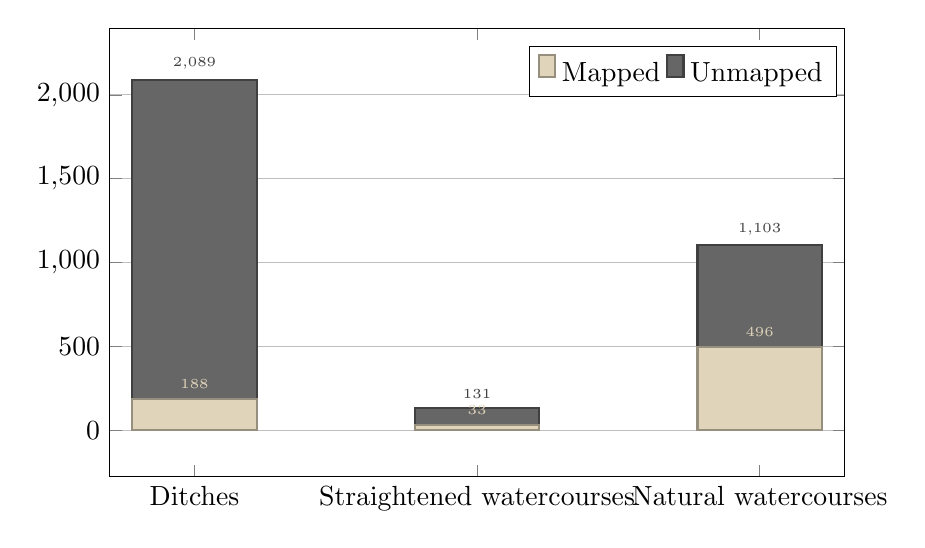
\begin{tikzpicture}
    \begin{axis}[
        width={0.9\textwidth},
        height={0.6\textwidth},
        ylabel={fluorescence},
        ybar stacked,
        ymajorgrids=true,
    	bar width=45pt,
    	nodes near coords,
    	every node near coord/.append style={font=\tiny},
        enlarge y limits={0.15},
        enlarge x limits=0.15,
        legend style={at={(0.78,0.96)},
          anchor=north,legend columns=-1},
        ylabel={{}},
        symbolic x coords={Ditches, Straightened  watercourses, Natural  watercourses},
        xtick=data,
        ytick={0,500,1000,1500,2000},
        x tick label style={rotate=0,anchor=north},
        ]
    \addplot+[ybar,color=custombeige,fill=custombeige,draw=custombeigeouter,thick] plot coordinates {(Ditches,188) (Straightened  watercourses,33) 
      (Natural  watercourses,496)};
    \addplot+[ybar,color=customgrayouter,fill=customgray,draw=customgrayouter,thick] plot coordinates {(Ditches,1901) (Straightened  watercourses,98) 
      (Natural  watercourses,607)};
    \legend{\strut Mapped, \strut Unmapped}
    \end{axis}
    \end{tikzpicture}
    \caption{\textbf{\DIFaddFL{Channel mapping status.}} \DIFaddFL{The bars indicate the number of observed channels in the National Inventory of Landscapes in Sweden's (NILS) line inventory of small watercourses (width $<$ 6 m). The colours of the bars indicate whether they are mapped or not on the Swedish Property map.}}
    \label{fig:watercoursebarplot}
\end{figure}

\DIFadd{Several previous studies have located ditches from remote sensing Light Detection and Ranging (LiDAR) data in smaller agricultural areas \mbox{%DIFAUXCMD
\citep{roelens, bailly} }\hspace{0pt}%DIFAUXCMD
or smaller forest areas (smaller than 2 $km^2$) \mbox{%DIFAUXCMD
\citep{rapinel, kiss}}\hspace{0pt}%DIFAUXCMD
, predominantly characterised by artificial drainage. In this study, however, we conduct a landscape-scale analysis in a mesoscale catchment. The study  catchment  is 68 $km^2$, representing diverse landscape features and geomorphological characteristics. Additionally, the forest landscape introduces many challenges that are not present when detecting ditches along roads or in agricultural areas. The canopy cover in forest areas prevents the use of satellite imagery or aerial photos, as well as lowers the quality of the }\DIFaddend digital elevation models (DEMs)\DIFdelbegin \DIFdel{and terrain indices provides a feasible means for spatially explicit assessment of ditches across a landscape. Previous researches  \mbox{%DIFAUXCMD
\citep{uppsala} }\hspace{0pt}%DIFAUXCMD
documented  }\DIFdelend \DIFaddbegin \DIFadd{, as fewer LiDAR points reach the ground, instead frequently catching in trees, bushes, or grass. Forest ditches are also generally not maintained to the same extent as agricultural or road ditches, often being overgrown or covered by windthrows or windsnaps. Using raw LiDAR point clouds to detect ditches, as \mbox{%DIFAUXCMD
\citet{roelens} }\hspace{0pt}%DIFAUXCMD
and \mbox{%DIFAUXCMD
\citet{bailly} }\hspace{0pt}%DIFAUXCMD
did in their studies can thus be problematic in a forest landscape, where a DEM constructed to map the points on the ground should be more suitable. \mbox{%DIFAUXCMD
\citet{cazorzi} }\hspace{0pt}%DIFAUXCMD
used a DEM with image processing techniques aimed at detecting the elongated ditch shapes and excluding large landscape features. This approach worked well for their open agricultural areas, but is difficult to generalise to a diverse forest landscape. Instead, we will focus on the topographical incision of the ditches in the DEM, which will be highlighted with a set of digital terrain indices. Previous studies have found }\DIFaddend that terrain indices such as \DIFdelbegin \DIFdel{Sky View Factor \mbox{%DIFAUXCMD
\citep{zaksek}}\hspace{0pt}%DIFAUXCMD
, Impoundment Index }\DIFdelend \DIFaddbegin \hyperref[skyviewfactor]{Sky View Factor} \DIFadd{\mbox{%DIFAUXCMD
\citep{zaksek}}\hspace{0pt}%DIFAUXCMD
, }\hyperref[impoundment]{Impoundment Index} \DIFaddend \citep{whiteboxtools} and High Pass Median Filter \citep{whiteboxtools} can \DIFdelbegin \DIFdel{efficiently  detect the ditches }\DIFdelend \DIFaddbegin \DIFadd{detect ditches in forest landscapes in some cases \mbox{%DIFAUXCMD
\citep{uppsala}}\hspace{0pt}%DIFAUXCMD
}\DIFaddend . However, different false positives and negatives \DIFdelbegin \DIFdel{may }\DIFdelend \DIFaddbegin \DIFadd{can }\DIFaddend be observed when examining each terrain index manually. \DIFdelbegin \DIFdel{Such inaccuracies and complexities are in part related to the Light Detection and Ranging (LiDAR ) measurements, the mainstay of high resolution DEM and terrain mapping, sometimes being interfered by trees, bushes, or grass - leaving gaps in the ditch model. The inaccuracies can also arise }\DIFdelend \DIFaddbegin \DIFadd{These inaccuracies can stem either from the gaps in the LiDAR scans, or }\DIFaddend from a poorly set threshold for the \DIFdelbegin \DIFdel{LiDAR derived terrain }\DIFdelend \DIFaddbegin \DIFadd{terrain index }\DIFaddend parameters. Thus, it would be useful to combine \DIFdelbegin \DIFdel{the terrain indices derived from high resolution LiDAR data }\DIFdelend \DIFaddbegin \DIFadd{these terrain indices }\DIFaddend to prune the weaknesses and amplify the strengths of each index \DIFdelbegin \DIFdel{and produce }\DIFdelend \DIFaddbegin \DIFadd{to produce a }\DIFaddend highly accurate detection of ditch networks. 

In this study, we \DIFdelbegin \DIFdel{first investigate the need for better maps of ditch networks, then we }\DIFdelend introduce a new method for the automated mapping of ditches by integrating multiple high resolution terrain indices \DIFdelbegin \DIFdel{(derived from LiDAR DEM) using a machine learning algorithm. We also examine which digital terrain indices are the most relevant for an accurate prediction of ditches. Several input variables for the model are calculated from the indices to place emphasis on the clear linear directional characteristics of ditches. These characteristics are also used when processing the model's output, in order to remove noise and other inconsistencies in the predictions. We use a supervised learning algorithm with labelled ditch data to automatically extract ditches from instances not before seen by the model. These instances are used as input variables to the algorithm, and consist of refined or raw digital terrain indices derived from a DEM. }%DIFDELCMD < 

%DIFDELCMD < %%%
\DIFdelend \DIFaddbegin \DIFadd{using a supervised learning approach. Several features and post-processing steps, specifically tailored for ditch detection are also developed and employed. These features aim to both highlight elongated shapes similarly to \mbox{%DIFAUXCMD
\citet{cazorzi}}\hspace{0pt}%DIFAUXCMD
, as well as include a map of the neighbouring area as \mbox{%DIFAUXCMD
\citet{roelens} }\hspace{0pt}%DIFAUXCMD
did in their study. }\DIFaddend We hypothesise that by combining the information from all the digital terrain indices using a machine learner (Random Forests), we can improve the detection of the ditches, compared to if a single \DIFdelbegin \DIFdel{index would be }\DIFdelend \DIFaddbegin \DIFadd{terrain index is }\DIFaddend used. To test this, we conduct a landscape-scale ditch detection analysis at the Krycklan Catchment in Sweden \citep{krycklancatchment}, where a high precision manual \DIFaddbegin \DIFadd{ditch }\DIFaddend mapping has been performed\DIFdelbegin \DIFdel{previously}\DIFdelend . This manual \DIFdelbegin \DIFdel{map }\DIFdelend \DIFaddbegin \DIFadd{mapping }\DIFaddend guided the model training and ground-truthing in our analysis and provided a test-bench for our methodology.
\DIFdelbegin \DIFdel{Previous studies \mbox{%DIFAUXCMD
\citep{roelens, bailly, rapinel, kiss} }\hspace{0pt}%DIFAUXCMD
that have located ditches from LiDAR data have worked on smaller areas (smaller than 2 $km^2$), predominantly characterised by artificial drainage. However, we herein conduct a landscape-scale analysis in a mesoscale catchment. The study  catchment  is 68 $km^2$, representing diverse landscape features and geomorphological characteristics.
}\DIFdelend 

\section{Materials and method}
\label{method}

\subsection{\DIFdelbegin \DIFdel{The need for better small scale channel mappings}%DIFDELCMD < \MBLOCKRIGHTBRACE
%DIFDELCMD < %%%
\DIFdel{To investigate the need for better maps of ditches and small stream channels we compared the data from a national field survey with available maps. The National Inventory of Landscapes in Sweden (NILS) has recorded small watercourses (width $<$ 6 m) by conducting a line inventory in 631 $5*5$ km squares randomly distributed in Sweden, to best capture a representative and varied sample of the Swedish landscape. The positions of the small watercourses from this inventory were compared with the watercourses on Swedish Property Map (1: 12 500) (allowing for an uncertainty in the positioning of up to 15 m, by snapping the point observations to the lines on the map) (}%DIFDELCMD < \hyperref[fig:watercoursebarplot]{Figure} %%%
\DIFdel{\ref{fig:watercoursebarplot}).
}%DIFDELCMD < 

%DIFDELCMD < %%%
\subsection{\DIFdel{Study area}}
%DIFAUXCMD
\addtocounter{subsection}{-1}%DIFAUXCMD
\DIFdel{In the }\DIFdelend \DIFaddbegin \DIFadd{Study area and dataset}}
\DIFadd{The quaternary deposits in the }\DIFaddend Krycklan Study Catchment \DIFdelbegin \DIFdel{the quaternary deposits }\DIFdelend are dominated by till (51\%) and sorted sediments (30\%). The catchment ranges in elevation from 114 to 405 m above sea level. Forest covers 87\% of the catchment, mires 9\%, thin soils 7\%, and rock outcrops 1\%. The land use is dominated by forestry; approximately 25\% of the Krycklan catchment has been protected since 1922, but  the rest of the area is mostly second growth forest \citep{krycklancatchment}.  \DIFdelbegin %DIFDELCMD < 

%DIFDELCMD < %%%
\DIFdelend A historical survey of the catchment (Gudrun Norstedt, unpublished) recorded  that the ditches in the catchment were dug between 1900 and 1993. Initially, the ditches were dug to drain the mires for hay production. Later on, wet areas were drained to attempt to turn them into productive forest lands \citep{paivanen}. However, research later showed that many of the drained mires were not productive for forestry due to lack of nutrients \citep{sikstrom}.

\DIFaddbegin \DIFadd{The LiDAR dataset used in this study was produced by TerraTec Sweden AB in August 2015, on demand of the Department of Forest Resource Management at the Swedish University of Agricultural Sciences, and is freely available online \mbox{%DIFAUXCMD
\citep{dataset}}\hspace{0pt}%DIFAUXCMD
. The average density of the dataset is 20 pulses per $m^2$. Ground point classification was performed with lasground (included in LAStools, a software suite produced by rapidlasso GmbH). The DEM was created with blast2dem (included in LAStools), with a cell size of $0.5*0.5$ m. Only ground points were imported to generate a DEM of the ground.
}

\DIFaddend \subsection{Digitising the ground truth}
\DIFdelbegin \DIFdel{A high resolution DEM was generated from LiDAR data, see }%DIFDELCMD < \hyperref[lidartodem]{'Data and codes availability statement'}%%%
\DIFdel{. To train and validate the machine learning models}\DIFdelend \DIFaddbegin \DIFadd{For training and validation}\DIFaddend , a vector layer of all ditches in the Krycklan Catchment \citep{krycklancatchment} was digitised. The study catchment comprises several types of ditches including road ditches, forest ditches, and agricultural ditches. A multidirectional hillshade of the 0.5 m DEM was calculated in ArcGIS Pro\DIFdelbegin \DIFdel{to locate the ditches. From }\DIFdelend \DIFaddbegin \DIFadd{, and from }\DIFaddend this layer, most of the ditches could be easily identified \DIFaddbegin \DIFadd{by a human}\DIFaddend . We conducted the digitisation at a scale of 1:600 to ensure \DIFaddbegin \DIFadd{that }\DIFaddend all the digitised ditches \DIFdelbegin \DIFdel{properly align }\DIFdelend \DIFaddbegin \DIFadd{are properly aligned with }\DIFaddend the actual ditch on the ground\DIFaddbegin \DIFadd{, }\DIFaddend and do not coincide with the edge of the banks. In addition, both current and historical records and orthophotos dating back to the 1960's were consulted to help locate all the ditches. In uncertain areas, the ditches were verified in the field. The \DIFdelbegin \DIFdel{stream network in }%DIFDELCMD < \hyperref[fig:swedenkrycklan]{Figure} %%%
\DIFdel{\ref{fig:swedenkrycklan} shows a network with a 8 hectare flow initiation threshold. The }\DIFdelend digitisation of the ditch networks showed that there are 107 km of road ditches and 208 km of forest/agricultural ditches in the catchment (\hyperref[fig:swedenkrycklan]{Figure} \ref{fig:swedenkrycklan}). The stream network in \hyperref[fig:swedenkrycklan]{Figure} \ref{fig:swedenkrycklan} \DIFdelbegin \DIFdel{, which represents }\DIFdelend \DIFaddbegin \DIFadd{shows a 197 km long network with a 8 hectare flow initiation threshold, representing }\DIFaddend median flow conditions\DIFdelbegin \DIFdel{, was 197 km}\DIFdelend .

\DIFdelbegin %DIFDELCMD < \begin{figure}
%DIFDELCMD <     %%%
\DIFdelendFL \DIFaddbeginFL \begin{figure}[!htb]
    \DIFaddendFL \centering
    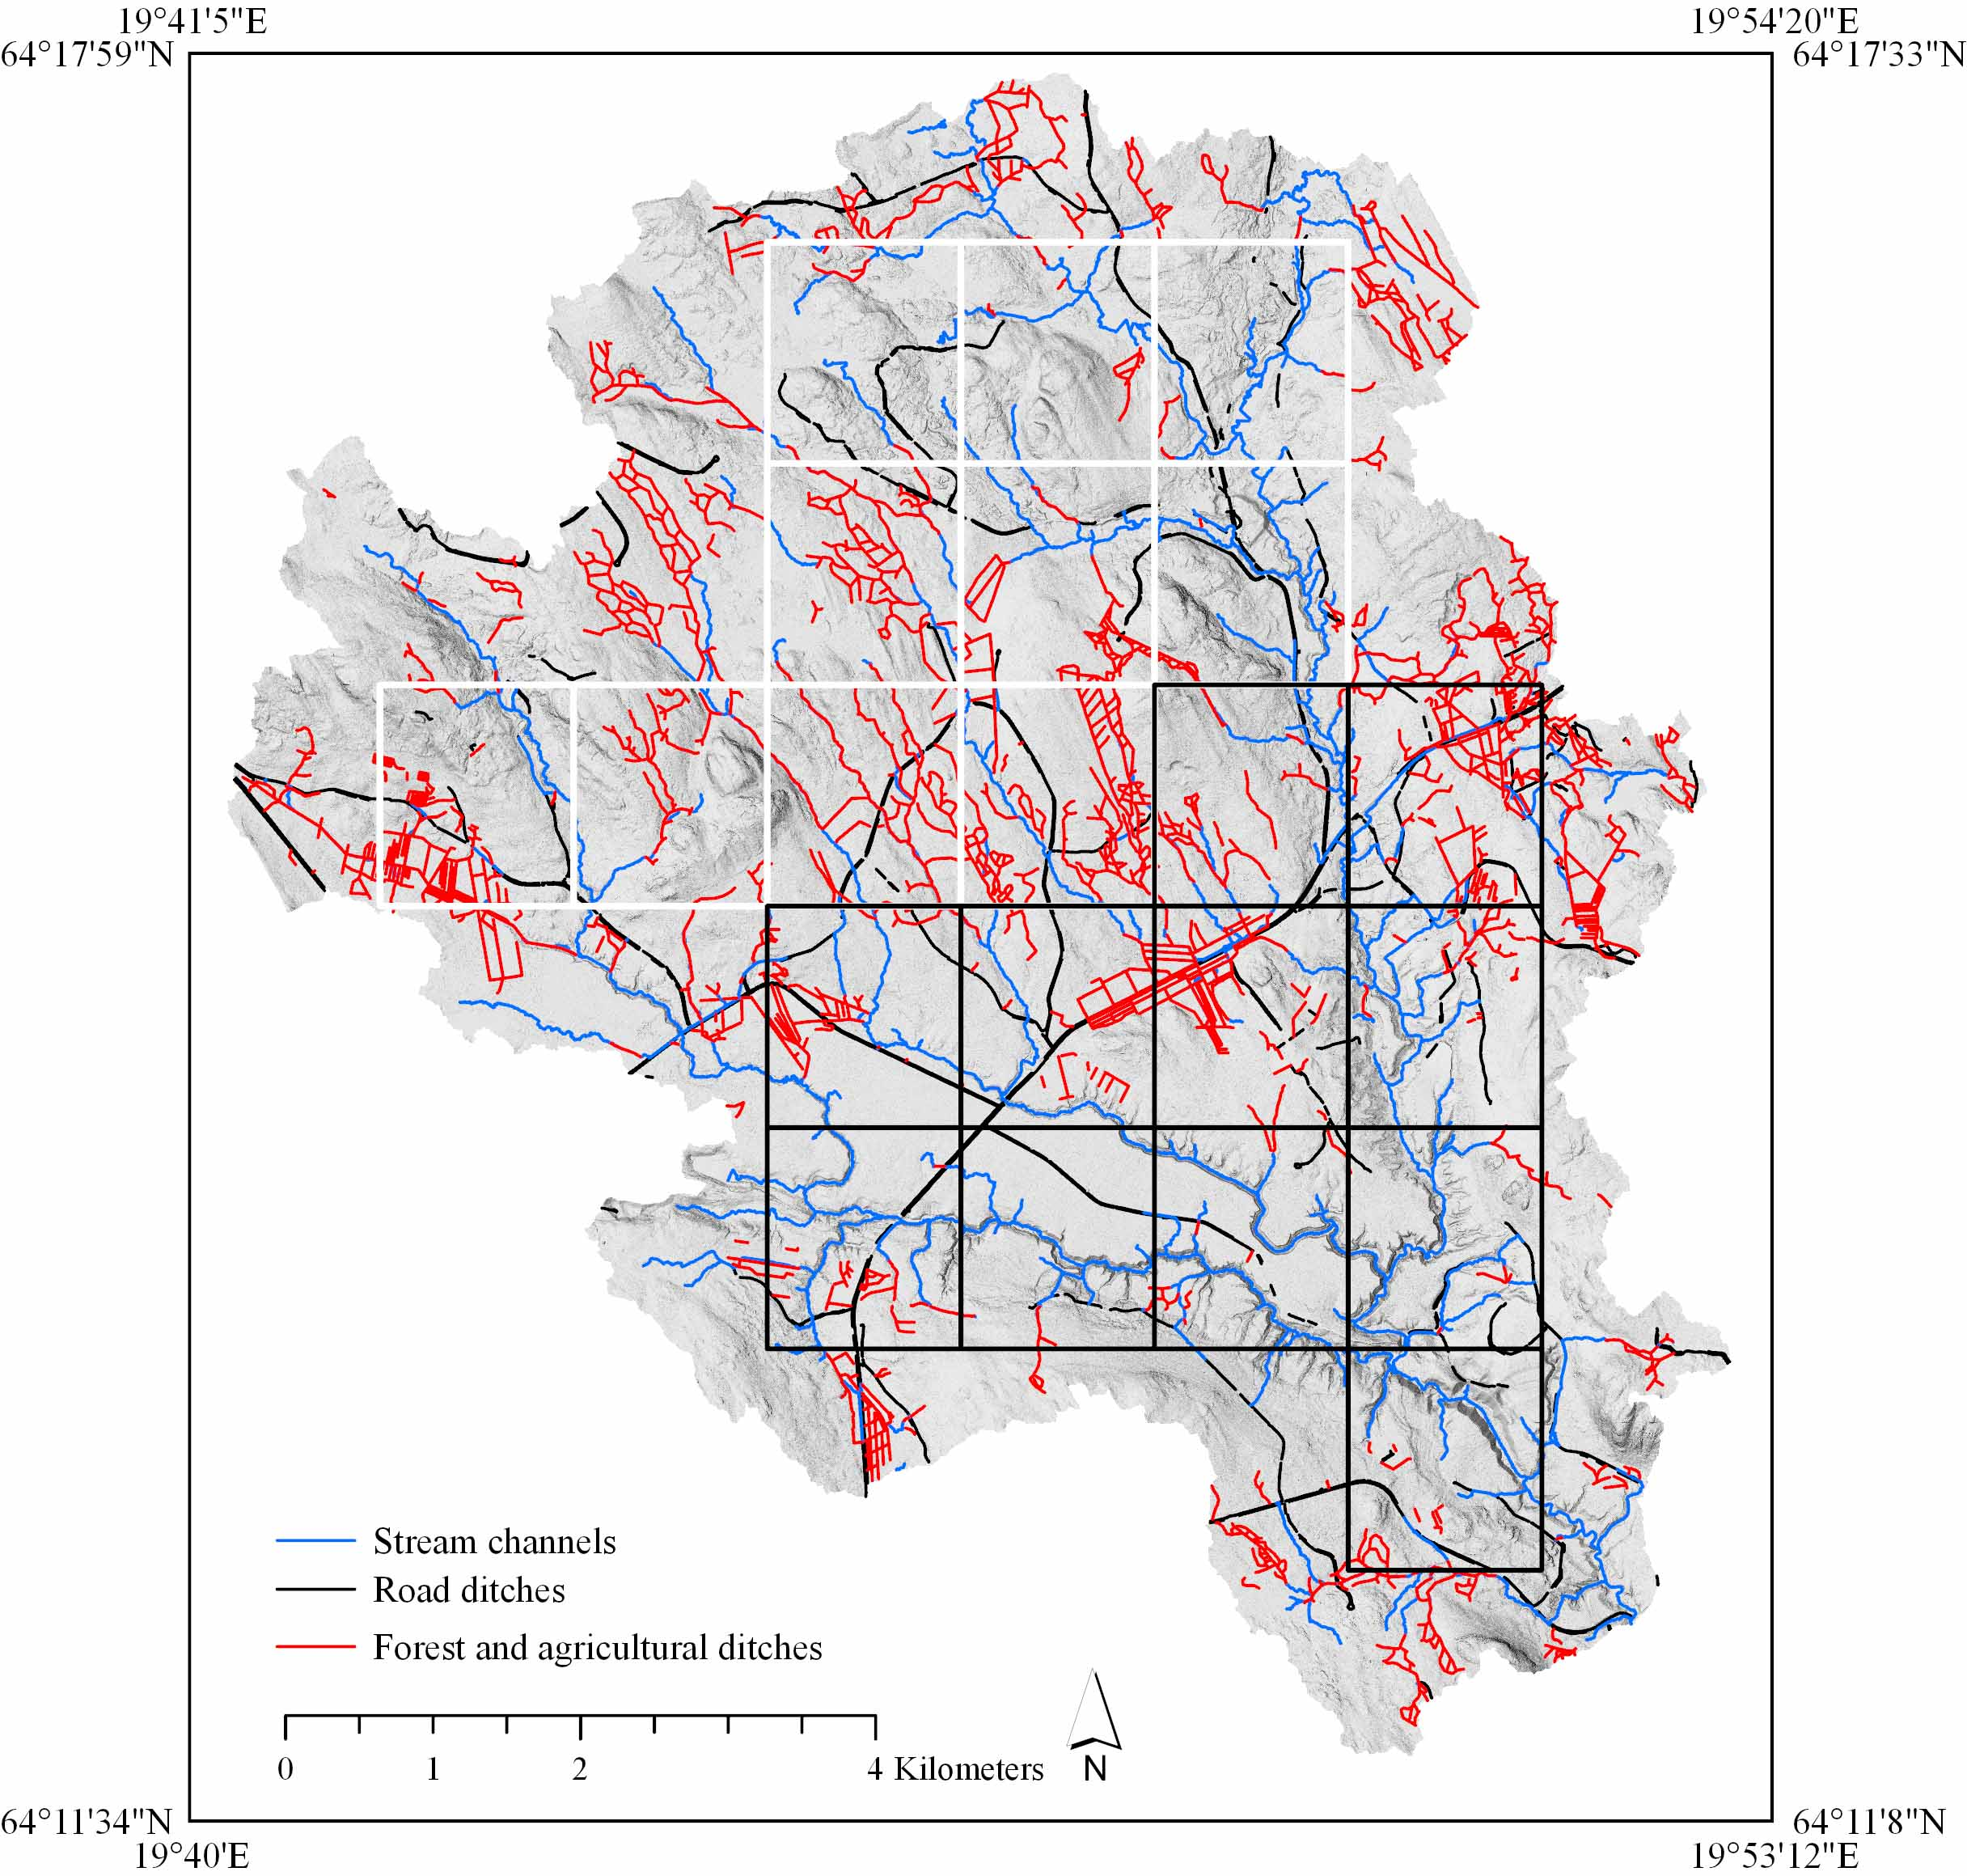
\includegraphics[width=1\linewidth]{./images/Krycklan_lo.jpg}
    \caption{\DIFdelbeginFL \DIFdelFL{Map of Krycklan showing }\DIFdelendFL \DIFaddbeginFL \textbf{\DIFaddFL{Krycklan channel map.}} \DIFaddFL{Shows }\DIFaddendFL ditches and stream channels \DIFaddbeginFL \DIFaddFL{in the Krycklan catchment}\DIFaddendFL , as well as our division into 21 subsections \DIFaddbeginFL \DIFaddFL{of $2997 \cdot 2620$ pixels (roughly 196 hectare each)}\DIFaddendFL . The 10 subsections with a white border were used for developing \DIFdelbeginFL \DIFdelFL{input variables }\DIFdelendFL \DIFaddbeginFL \DIFaddFL{features }\DIFaddendFL and optimising parameters before the experiment. The 11 subsections with a black border were used in the experiment for evaluation with 11-fold cross validation.\DIFdelbeginFL \DIFdelFL{Each rectangular subsection represents $2997 \cdot 2620$ pixels (roughly 196 hectare).}\DIFdelendFL }
    \label{fig:swedenkrycklan}
\end{figure}

From the ditch mapping, the vector layer was rasterised \DIFdelbegin \DIFdel{so that it could be compared to the automatically derived ditches from the }\DIFdelend \DIFaddbegin \DIFadd{with a resolution of }\DIFaddend $0.5*0.5$ \DIFdelbegin \DIFdel{m DEM}\DIFdelend \DIFaddbegin \DIFadd{metres for use as a ground-truth for our ditch detector}\DIFaddend . Our field observations have shown that \DIFdelbegin \DIFdel{the  width of most ditches within the catchment ranges }\DIFdelend \DIFaddbegin \DIFadd{most of the ditches in the catchment range }\DIFaddend between 0.5 and 3.5 \DIFdelbegin \DIFdel{m}\DIFdelend \DIFaddbegin \DIFadd{metres in width}\DIFaddend . To ensure that \DIFdelbegin \DIFdel{the model received }\DIFdelend all ditch pixels \DIFdelbegin \DIFdel{correctly }\DIFdelend \DIFaddbegin \DIFadd{were labelled correctly for the model }\DIFaddend in the training phase, we \DIFdelbegin \DIFdel{widened the ditches so that }\DIFdelend \DIFaddbegin \DIFadd{labelled }\DIFaddend all pixels within \DIFdelbegin \DIFdel{a radius of }\DIFdelend three pixels (1.5 metres) of the vectors \DIFdelbegin \DIFdel{were labelled }\DIFdelend as ditch pixels\DIFdelbegin \DIFdel{. }\DIFdelend \DIFaddbegin \DIFadd{, making the labels 3.5 metres wide (}\DIFaddend \hyperref[fig:ditchpreprocess]{Figure} \ref{fig:ditchpreprocess}\DIFdelbegin %DIFDELCMD < \hyperref[fig:ditchpreprocess]{a} %%%
\DIFdel{shows the ditches rasterised from vectors and }%DIFDELCMD < \hyperref[fig:ditchpreprocess]{Figure} %%%
\DIFdel{\ref{fig:ditchpreprocess} }%DIFDELCMD < \hyperref[fig:ditchpreprocess]{b} %%%
\DIFdel{shows the ditches after widening. The data in }%DIFDELCMD < \hyperref[fig:ditchpreprocess]{Figure} %%%
\DIFdel{\ref{fig:ditchpreprocess} }%DIFDELCMD < \hyperref[fig:ditchpreprocess]{b} %%%
\DIFdel{is the labelled data that was used to train the machine learning models. The ditches all have a generalised width based on a perceived average of ditch width in the area. }\DIFdelend \DIFaddbegin \DIFadd{). }\DIFaddend Due to all ditches varying in width, it was impossible to produce a perfect representation of each ditch, but this widening helped ensure that almost all ditch pixels were covered by the labels. \DIFdelbegin %DIFDELCMD < 

%DIFDELCMD < %%%
\DIFdelend To match the labels with \DIFdelbegin \DIFdel{out }\DIFdelend \DIFaddbegin \DIFadd{our }\DIFaddend predictions (where we downscale the predictions into grids to remove outliers), the ground-truth was also downscaled into grids of $6*6$ pixels (9 $m^2$) each \DIFdelbegin \DIFdel{. Each grid cell that contained }\DIFdelend \DIFaddbegin \DIFadd{by labelling each grid cell containing }\DIFaddend at least 25\% ditch pixels \DIFdelbegin \DIFdel{was labelled }\DIFdelend as a ditch \DIFdelbegin \DIFdel{, see }\DIFdelend \DIFaddbegin \DIFadd{(}\DIFaddend \hyperref[fig:ditchpreprocess]{Figure} \ref{fig:ditchpreprocess} \hyperref[fig:ditchpreprocess]{c}\DIFdelbegin \DIFdel{. This layer was used to ground-truth the machine learning models.
}\DIFdelend \DIFaddbegin \DIFadd{).
}\DIFaddend 

\begin{figure} [\DIFdelbeginFL \DIFdelFL{htb!}\DIFdelendFL \DIFaddbeginFL \DIFaddFL{!htb}\DIFaddendFL ]
    \centering
    \DIFdelbeginFL %DIFDELCMD < \subfigure[]{
%DIFDELCMD <         \resizebox*{4.5cm}{!}{\includegraphics{./images/publ_ditch_preprocess_A_lo.jpg}}}%%%
\DIFdelFL{\hspace{5pt}
    }%DIFDELCMD < \subfigure[]{
%DIFDELCMD <         \resizebox*{4.5cm}{!}{\includegraphics{./images/publ_ditch_preprocess_B_lo.jpg}}}
%DIFDELCMD <     \subfigure[]{
%DIFDELCMD <         \resizebox*{4.5cm}{!}{\includegraphics{./images/publ_ditch_preprocess_C_lo.jpg}}}
%DIFDELCMD <     %%%
\DIFdelendFL \DIFaddbeginFL \subfigure[]{
        \resizebox*{3.5cm}{!}{\includegraphics{./images/publ_ditch_preprocess_A_lo.jpg}}}\DIFaddFL{\hspace{5pt}
    }\subfigure[]{
        \resizebox*{3.5cm}{!}{\includegraphics{./images/publ_ditch_preprocess_B_lo.jpg}}}
    \subfigure[]{
        \resizebox*{3.5cm}{!}{\includegraphics{./images/publ_ditch_preprocess_C_lo.jpg}}}
    \DIFaddendFL \caption{\DIFdelbeginFL \DIFdelFL{Processing of ditch labels. }\DIFdelendFL \DIFaddbeginFL \textbf{\DIFaddFL{Processing of ditch labels.}} \DIFaddendFL \textbf{a: }Rasterised ditches with a width of one pixel. \textbf{b: }Ditches after a widening process, seven pixels (3.5 metres) wide. Used as \DIFdelbeginFL \DIFdelFL{input }\DIFdelendFL \DIFaddbeginFL \DIFaddFL{labels }\DIFaddendFL when training the models. \textbf{c: }Ditches after a grid zone conversion. Used for evaluating the results from the ditch detector.} \label{sample-figure}
    \label{fig:ditchpreprocess}
\end{figure}

\subsection{Extracting ditches with digital terrain indices}
From the DEM, several digital terrain indices were calculated\DIFdelbegin \DIFdel{. The strengths and weaknesses of these indices have been obtained from observing their performance in different topological environments}\DIFdelend :
\begin{itemize} \label{data_attributes}

  \item \textbf{Sky View Factor} \DIFaddbegin \label{skyviewfactor} \DIFaddend \newline
    The Sky View Factor represents how much of the sky that is visible from a certain point on the ground \citep{zaksek}. A point \DIFdelbegin \DIFdel{in }\DIFdelend \DIFaddbegin \DIFadd{inside }\DIFaddend a ditch would \DIFdelbegin \DIFdel{yield }\DIFdelend \DIFaddbegin \DIFadd{produce }\DIFaddend a low value, as more of the sky is obscured by the ditch bank. \DIFdelbegin \DIFdel{However, it }\DIFdelend \DIFaddbegin \DIFadd{Sky View Factor }\DIFaddend tends to produce false positives in steep terrain. The \DIFdelbegin \DIFdel{Sky View Factor }\DIFdelend \DIFaddbegin \DIFadd{index }\DIFaddend was calculated in SAGA GIS, using a search radius of 10 metres to ensure that it was large enough to capture the ditches, but small enough to not include large scale topographical features such as hills.

  \item \textbf{Impoundment Index} \DIFaddbegin \label{impoundment} \DIFaddend \newline
    The Impoundment Index in Whitebox Tools \citep{whiteboxtools} can be used as a measure of flow constriction, which is useful for mapping channels \DIFdelbegin \DIFdel{, }\DIFdelend such as ditches. When tuned to output the flooded volume, it effectively maps the area and average depth of the reservoir that would be created by placing a dam of a user-specified length at each grid cell in the DEM. Here, we used dam height calculated with a dam length of 3 metres to \DIFaddbegin \DIFadd{attempt to }\DIFaddend cover the entire ditches. Typical false positives with this \DIFdelbegin \DIFdel{method }\DIFdelend \DIFaddbegin \DIFadd{index }\DIFaddend are natural stream channels with a clear incised channel.

  \item \textbf{High Pass Median Filter} \DIFaddbegin \label{hpmf} \DIFaddend \newline
    High Pass Median Filters (HPMF) highlight ditches by indicating local depressions (such as ditches) in the DEM by subtracting the value at the grid cell at the centre of the window from the median value in the window. Typical false positives with this index are small hollows. HPMF was calculated using Whitebox Tools \citep{whiteboxtools} with a window size of $4.5 * 4.5$ m. 

    \item \textbf{Slope} \DIFaddbegin \label{slope} \DIFaddend \newline
    The Slope index represents the degree of slope at a certain point, with a value ranging from $0^{\circ}$ to $90^{\circ}$ \DIFaddbegin \DIFadd{with no information about the direction of the slope}\DIFaddend . It was calculated on the 0.5 m grid, using ArcGIS \citep{EsriArcGisBook}.
\DIFdelbegin \DIFdel{This index contains no information about the direction of the slope.
}\DIFdelend \end{itemize}

\DIFdelbegin \subsubsection{\DIFdel{Thresholding the digital terrain indices}}
%DIFAUXCMD
\addtocounter{subsubsection}{-1}%DIFAUXCMD
\DIFdelend To benchmark our method against a non-machine learning method, we binarised the original four digital terrain indices using thresholds. Different threshold values were tested and the value that yielded the highest Cohen's Kappa score for each respective index was chosen. This test was conducted for the 11 subsections described in \DIFdelbegin \DIFdel{\ref{trainingvalidationdatasets}. The Sky View Factor index }\DIFdelend \DIFaddbegin \hyperref[trainingvalidationdatasets]{section} \DIFadd{\ref{trainingvalidationdatasets}. }\hyperref[skyviewfactor]{Sky View Factor} \DIFaddend was classified to only include values below 0.955, the \DIFdelbegin \DIFdel{Impoundment Index }\DIFdelend \DIFaddbegin \hyperref[impoundment]{Impoundment Index} \DIFaddend Dam Height using values above 0.27 $m$, \DIFdelbegin \DIFdel{the HPMF index }\DIFdelend \DIFaddbegin \hyperref[hpmf]{HPMF} \DIFaddend using values below -0.18 m, and the \DIFdelbegin \DIFdel{Slope }\DIFdelend \DIFaddbegin \hyperref[slope]{Slope} \DIFaddend index using values above $14 ^{\circ}$ (\DIFdelbegin \DIFdel{Table 2}\DIFdelend \DIFaddbegin \autoref{recreatedpredictionperformance}\DIFaddend ).

\subsection{Data preparation}

\subsubsection{\DIFdelbegin \DIFdel{Processing the digital terrain indices}\DIFdelend \DIFaddbegin \DIFadd{Feature engineering}\DIFaddend }
\DIFdelbegin \DIFdel{We examined how different  input variables affected the prediction of the machine learning models. Several possible data manipulation methods could theoretically produce a better prediction. To improve the prediction, steps were taken where neighbouring pixels were included to }\DIFdelend \DIFaddbegin 

\DIFadd{The digital terrain indices provided a satisfactory foundation for the models, but could not always generalise well to outlier situations. To }\DIFaddend give a representation of the area surrounding a specific pixel, \DIFdelbegin \DIFdel{similar to the approach of \mbox{%DIFAUXCMD
\citet{roelens}}\hspace{0pt}%DIFAUXCMD
. 
}%DIFDELCMD < 

%DIFDELCMD < %%%
\DIFdel{The digital terrain indices provided a satisfactory foundation for the models, but lacked in the generalisability of their predictions. More diverse input variables were extracted }\DIFdelend \DIFaddbegin \DIFadd{we extracted more diverse features }\DIFaddend using simple statistical aggregates such as mean, median, min, max, and standard deviation \DIFdelbegin \DIFdel{. Using these statistical aggregations with the help of neighbouring areas around pixels }\DIFdelend \DIFaddbegin \DIFadd{in different circular radii around the pixel (similar to the approach of \mbox{%DIFAUXCMD
\citet{roelens}}\hspace{0pt}%DIFAUXCMD
). This }\DIFaddend aided in pruning pixels with outlier values, often smoothing out the data to represent ditches more accurately on a per-pixel basis \DIFdelbegin \DIFdel{. These variables were calculated by gathering all data points in different circular radii around the studied pixel, before computing one of the statistical aggregations }\DIFdelend (\hyperref[fig:features]{Figure} \ref{fig:features}: \hyperref[fig:features]{b}, \hyperref[fig:features]{c}, \hyperref[fig:features]{f}, and \hyperref[fig:features]{g}). \DIFdelbegin %DIFDELCMD < 

%DIFDELCMD < %%%
\DIFdel{In addition to the general input variables, a number of custom input variables were also developed.  Some of these custom variables were produced by statistical aggregation of multiple indices, whereas in some cases, they were }\DIFdelend \DIFaddbegin \DIFadd{Additionally, several features were }\DIFaddend generated by using thresholds \DIFaddbegin \DIFadd{on one or multiple indices }\DIFaddend to exclude, lower, or amplify the values of pixels that indicated ditches or non-ditches (\hyperref[fig:features]{Figure} \ref{fig:features}: \hyperref[fig:features]{d} and \hyperref[fig:features]{h}).

\DIFdelbegin \DIFdel{Both HPMF and Sky View Factor were used with }\DIFdelend \DIFaddbegin \DIFadd{Features were generated for both }\hyperref[hpmf]{HPMF} \DIFadd{and }\hyperref[skyviewfactor]{Sky View Factor} \DIFadd{using }\DIFaddend the image processing \textit{gabor filter}, which can be used to detect lines of a certain orientation in an image \citep{gabor}. 30 Gabor filters which were rotated in different angles and with different frequencies were combined to detect lines, amplifying ditches by utilising the fact that ditches have a linear elongated shape (\hyperref[fig:features]{Figure} \ref{fig:features}: \hyperref[fig:features]{e}).

\label{impoundmentstreamremoval}
\DIFdelbegin \DIFdel{The raw Impoundment Index dam height }\DIFdelend \DIFaddbegin \DIFadd{In an attempt to exclude streams from the predictions, the }\hyperref[impoundment]{Impoundment Index} \DIFaddend was used to \DIFdelbegin \DIFdel{create a mask , attempting to mask out streams, but retain ditches. Only }\DIFdelend \DIFaddbegin \DIFadd{mask out }\DIFaddend areas with a \DIFdelbegin \DIFdel{relatively high value, }\DIFdelend \DIFaddbegin \DIFadd{very large dam height (}\DIFaddend which would indicate that \DIFdelbegin \DIFdel{these areas }\DIFdelend \DIFaddbegin \DIFadd{the area }\DIFaddend most likely contained \DIFdelbegin \DIFdel{streams, were masked out. After widening the resulting area, this mask was used to remove streams from all the aforementioned custom input variables}\DIFdelend \DIFaddbegin \DIFadd{a stream). This mask was applied on several features to smooth out the values under the mask}\DIFaddend , generating one new \DIFdelbegin \DIFdel{input variable from each }\DIFdelend \DIFaddbegin \DIFadd{feature from each of them}\DIFaddend . The features marked with \textit{streams removed} in \hyperref[featuretable]{Table} \ref{featuretable} make use of this filter (\hyperref[fig:features]{Figure} \ref{fig:features}: \hyperref[fig:features]{i}).

Overall, 81 \DIFdelbegin \DIFdel{input variables }\DIFdelend \DIFaddbegin \DIFadd{features }\DIFaddend were extracted from the terrain indices. In a pilot study, we compared several different algorithms (Random Forests, Extreme Gradient Boosting, Naive Bayes, and Support Vector Machines), and it was found that Random Forests produced the most accurate results\DIFdelbegin \DIFdel{, here we therefore only present the results from the Random Forest model}\DIFdelend . We then conducted a sub-experiment \DIFaddbegin \DIFadd{using Random Forests' feature importance }\DIFaddend to find the best \DIFdelbegin \DIFdel{input variables}\DIFdelend \DIFaddbegin \DIFadd{features}\DIFaddend , as well as the optimal number of \DIFdelbegin \DIFdel{variables to use. The variable importance score in Random Forests was used to select the most important input variables and it was found that using the top }\DIFdelend \DIFaddbegin \DIFadd{features to use, resulting in a final feature set of }\DIFaddend 40 \DIFdelbegin \DIFdel{input variables produced the best results}\DIFdelend \DIFaddbegin \DIFadd{features (}\autoref{featuretable}\DIFadd{)}\DIFaddend .

\begin{figure} [!htb]
    \centering
    \DIFdelbeginFL %DIFDELCMD < \subfigure[]{
%DIFDELCMD <         \resizebox*{4cm}{!}{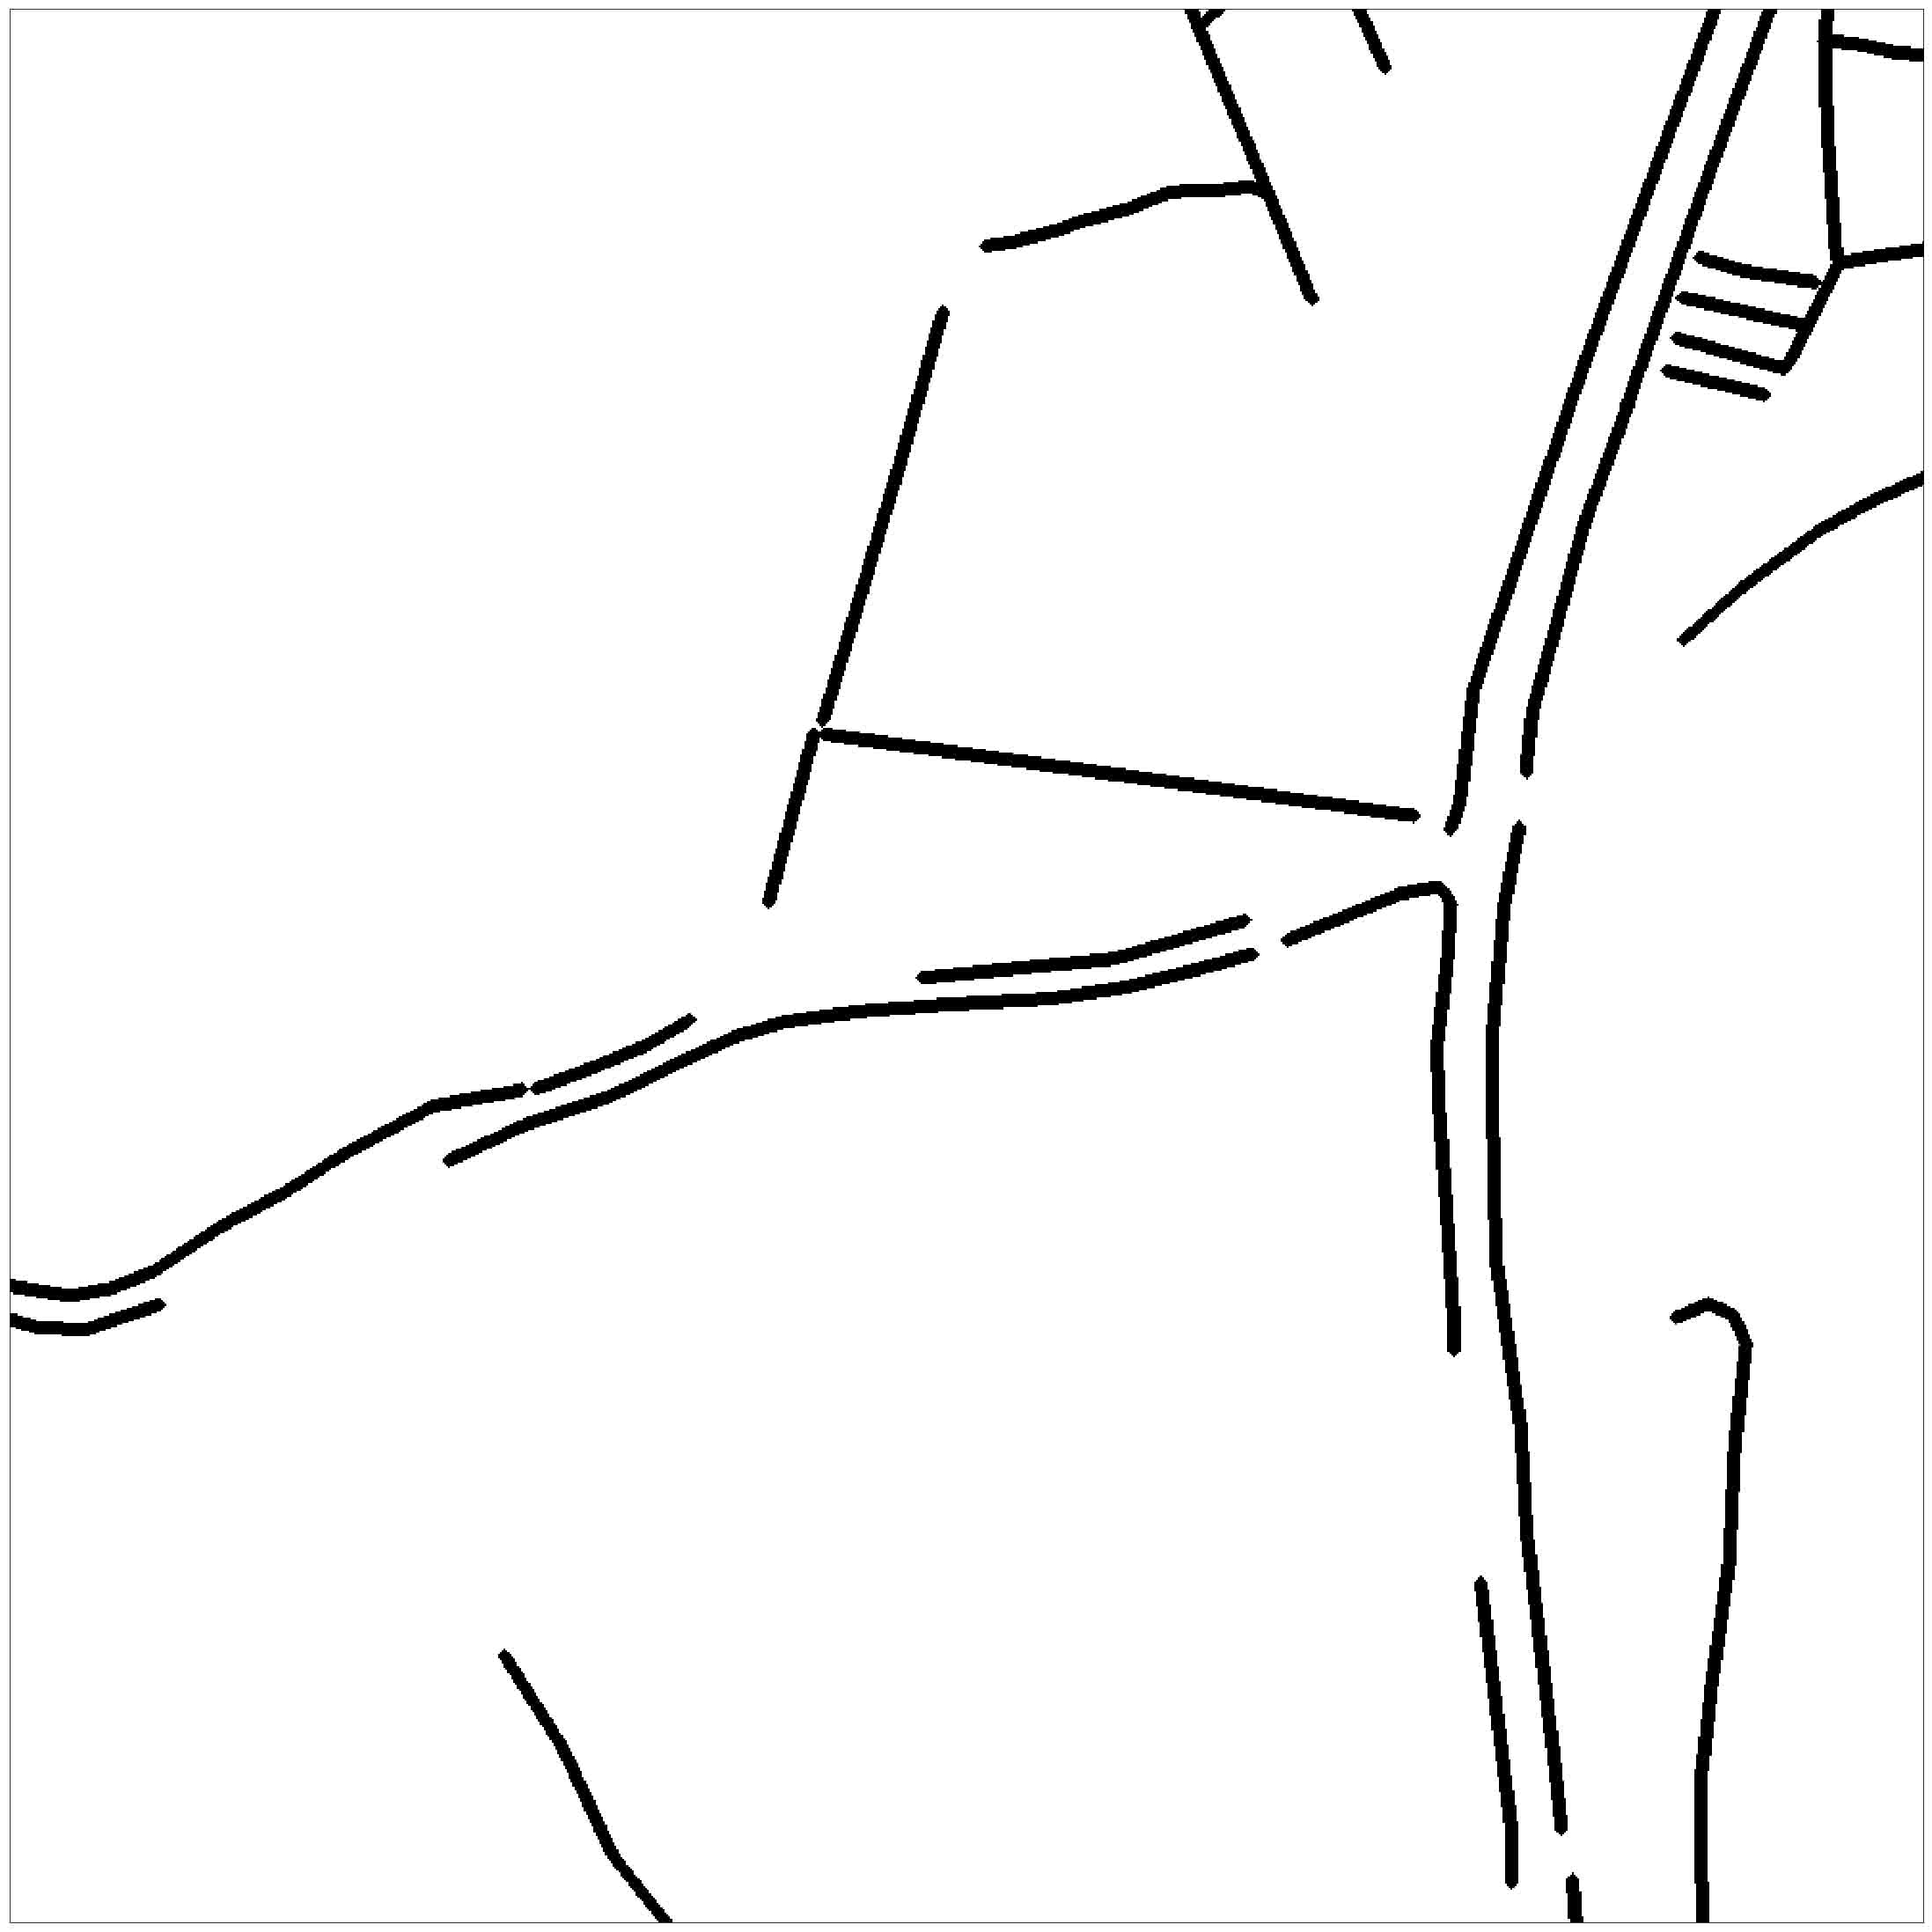
\includegraphics{./images/feature_a_lo.jpg}}}%%%
\DIFdelFL{\hspace{5pt}
    }%DIFDELCMD < \subfigure[]{
%DIFDELCMD <         \resizebox*{4cm}{!}{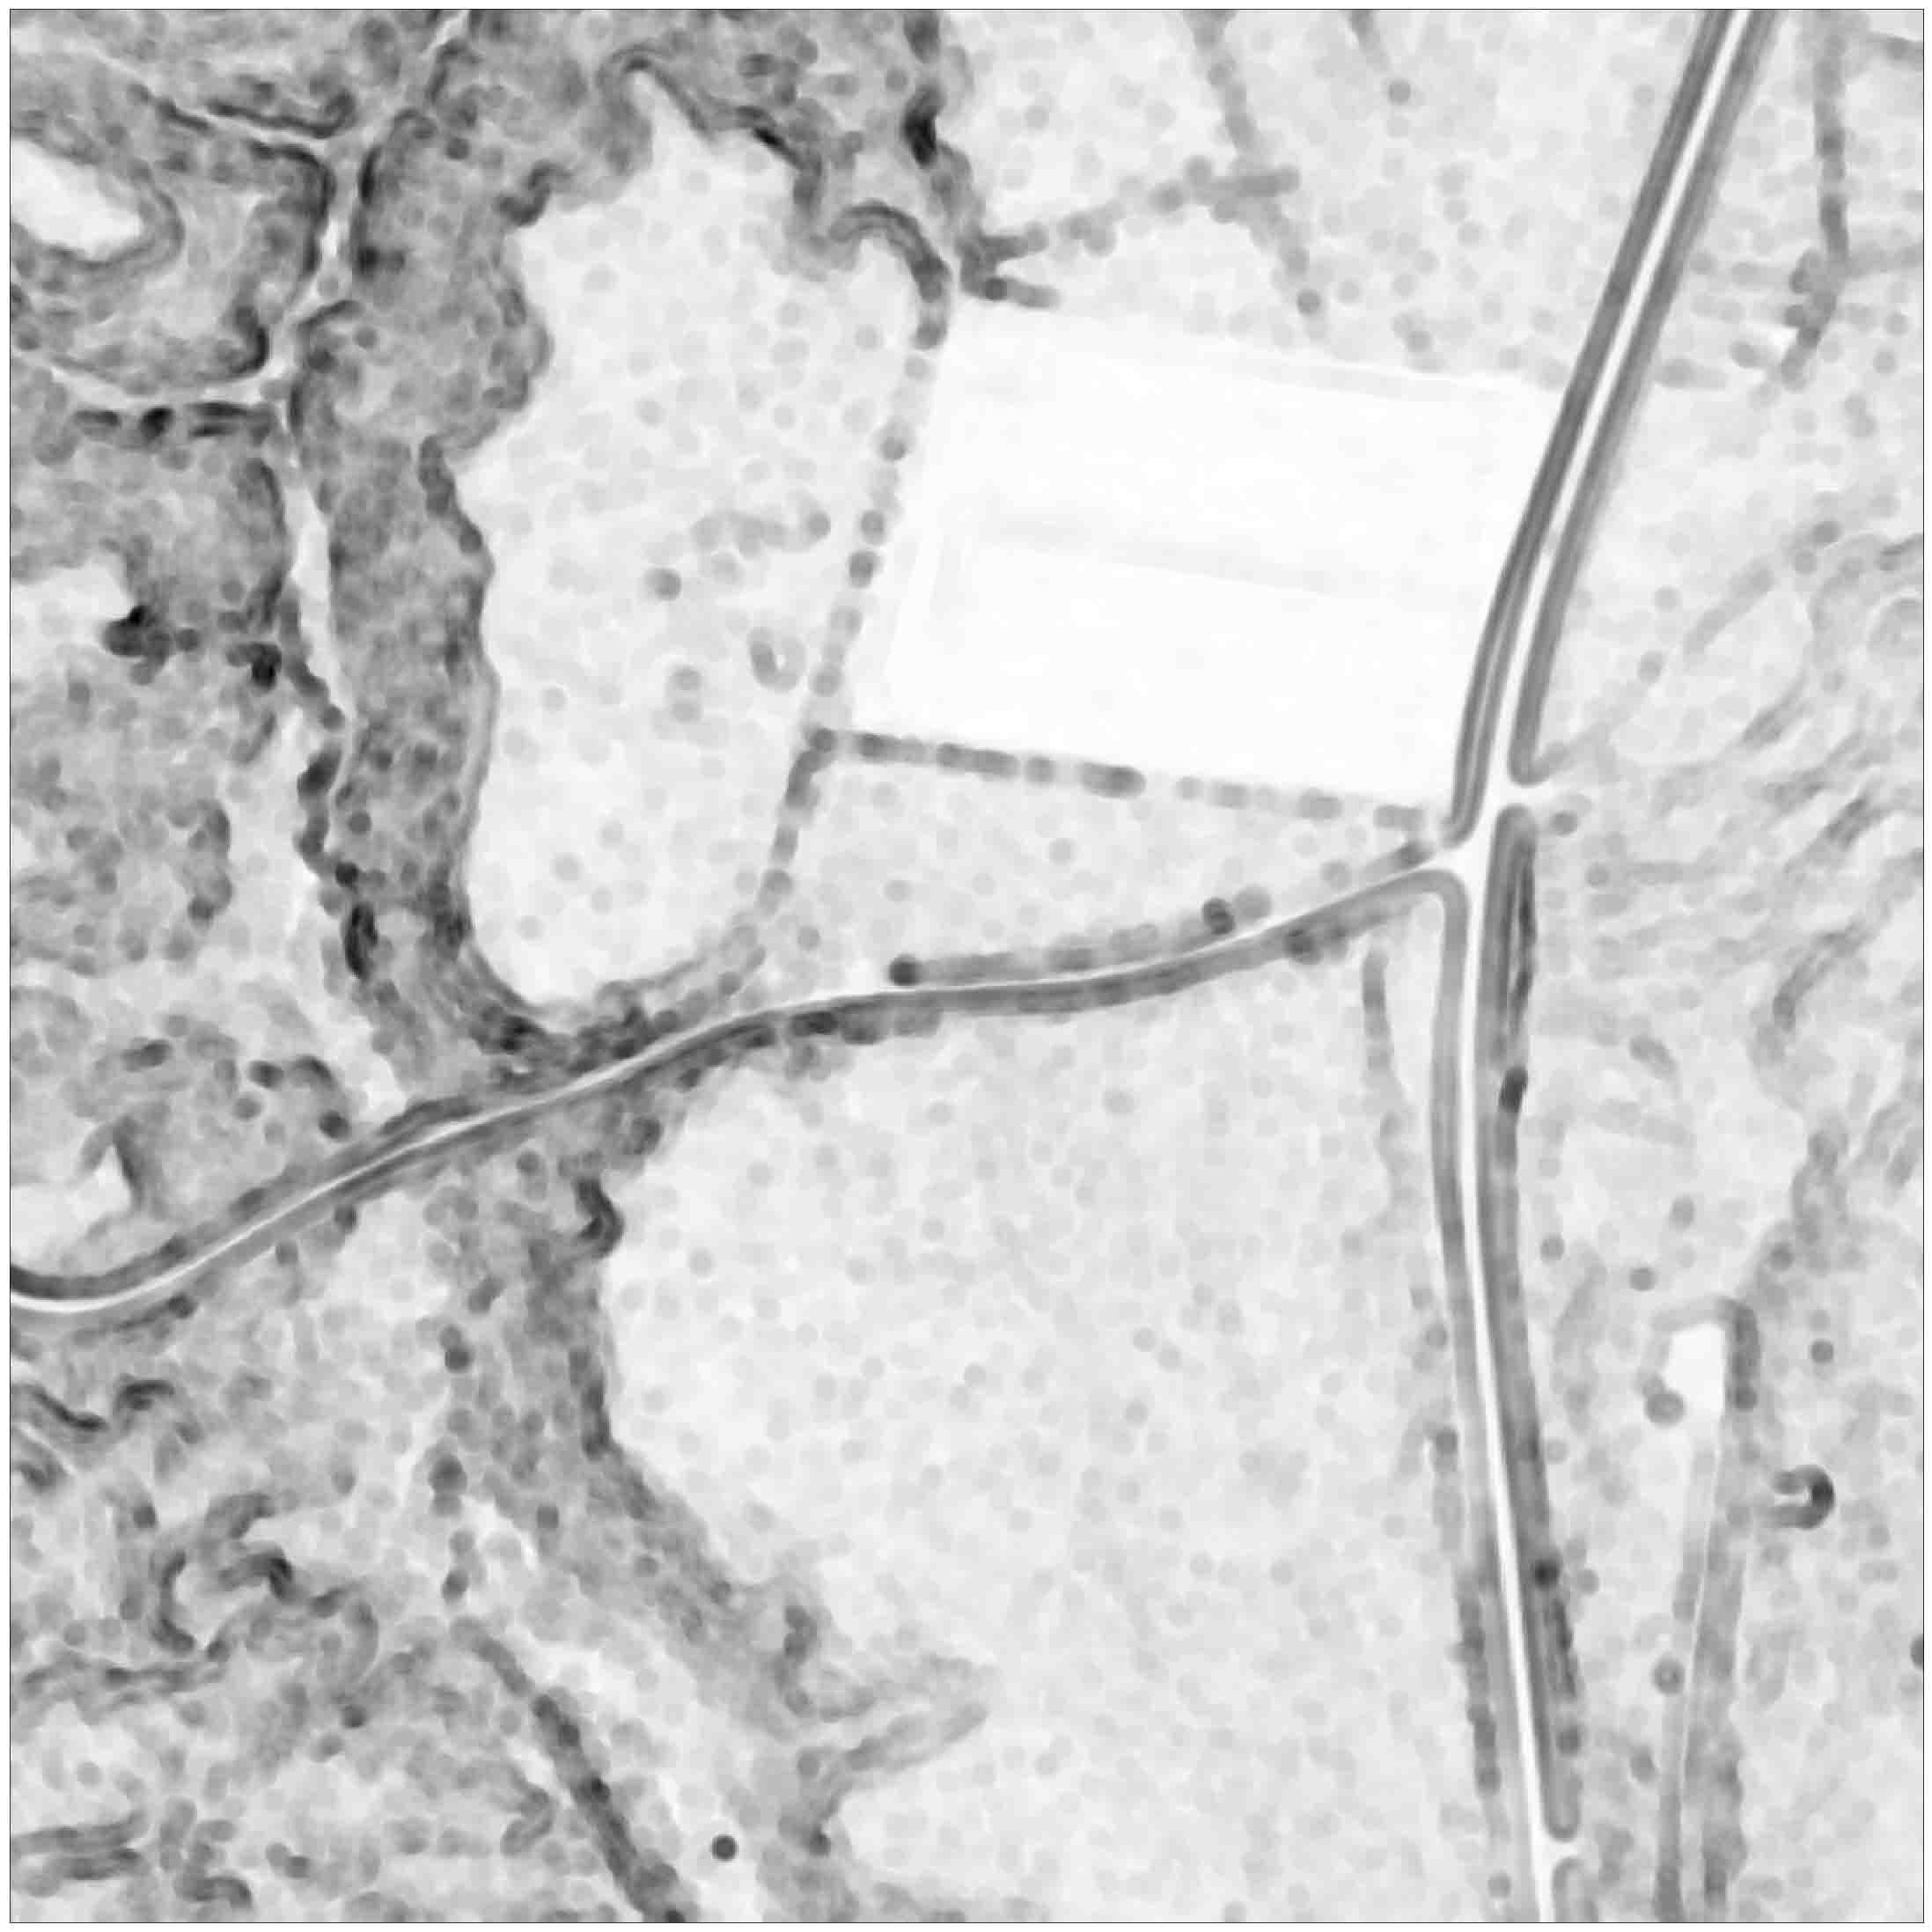
\includegraphics{./images/feature_b_lo.jpg}}}
%DIFDELCMD <     \subfigure[]{
%DIFDELCMD <         \resizebox*{4cm}{!}{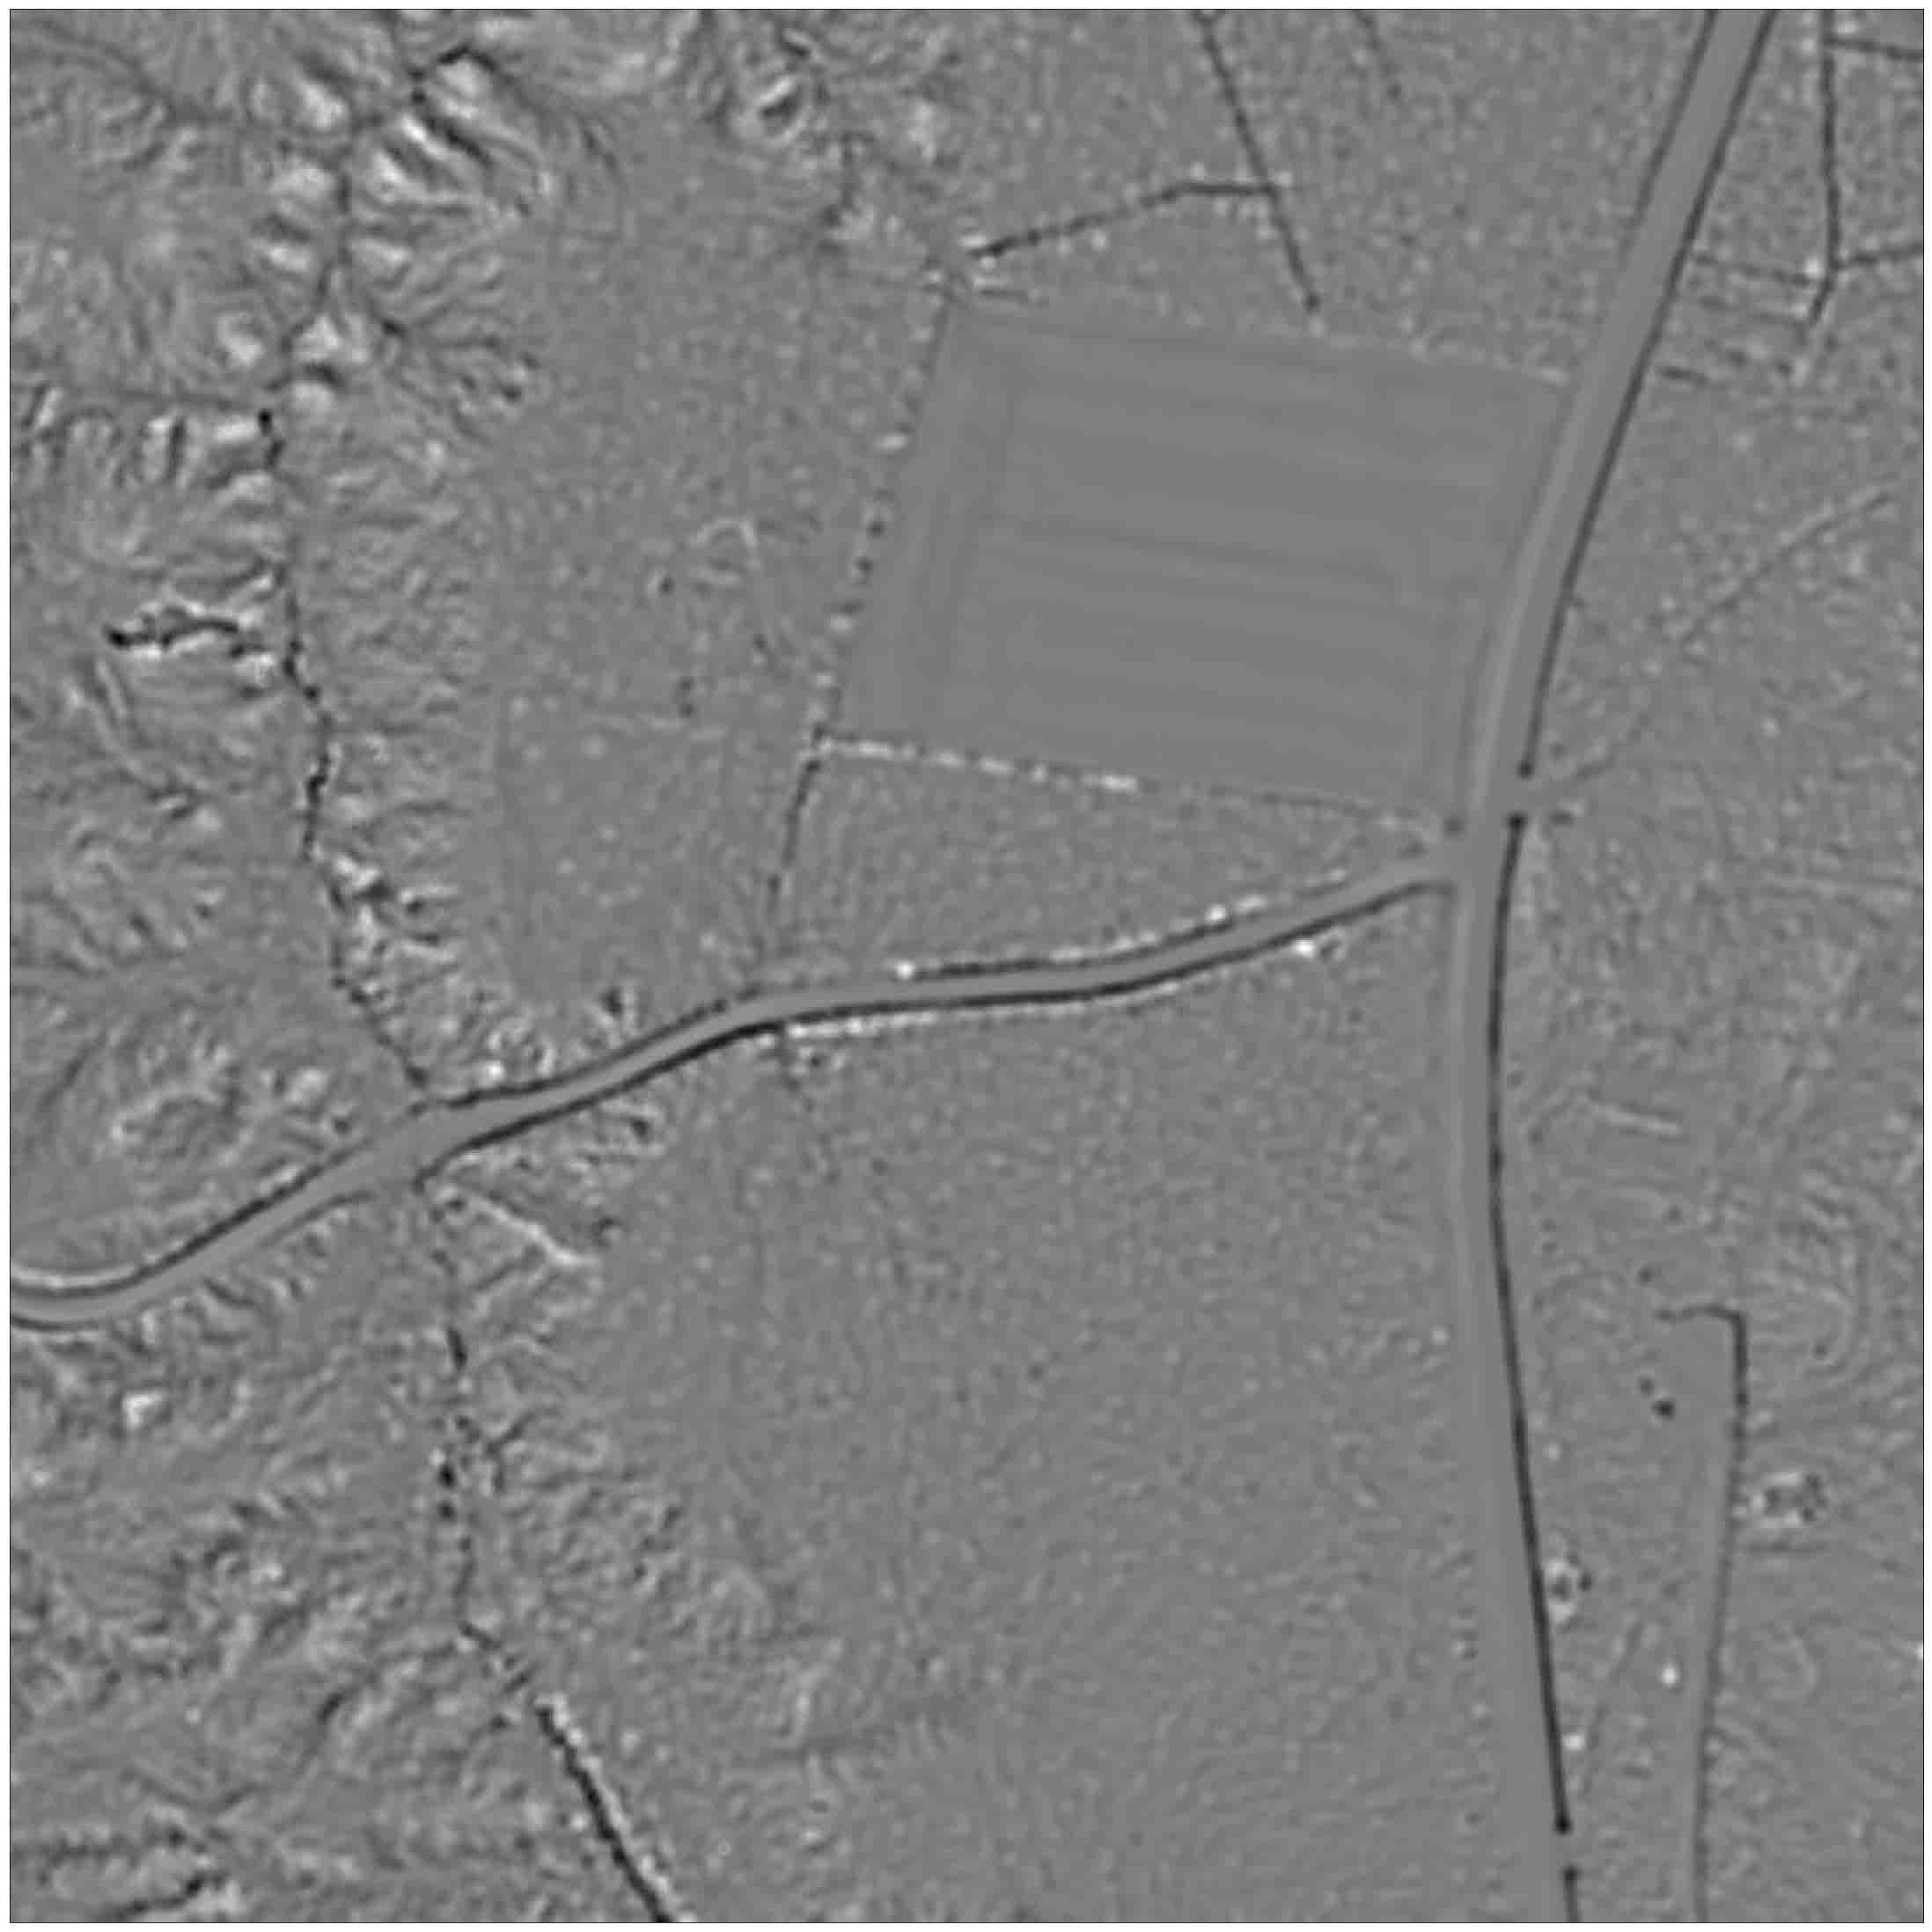
\includegraphics{./images/feature_c_lo.jpg}}}%%%
\DIFdelFL{\hspace{5pt}
    }%DIFDELCMD < \subfigure[]{
%DIFDELCMD <         \resizebox*{4cm}{!}{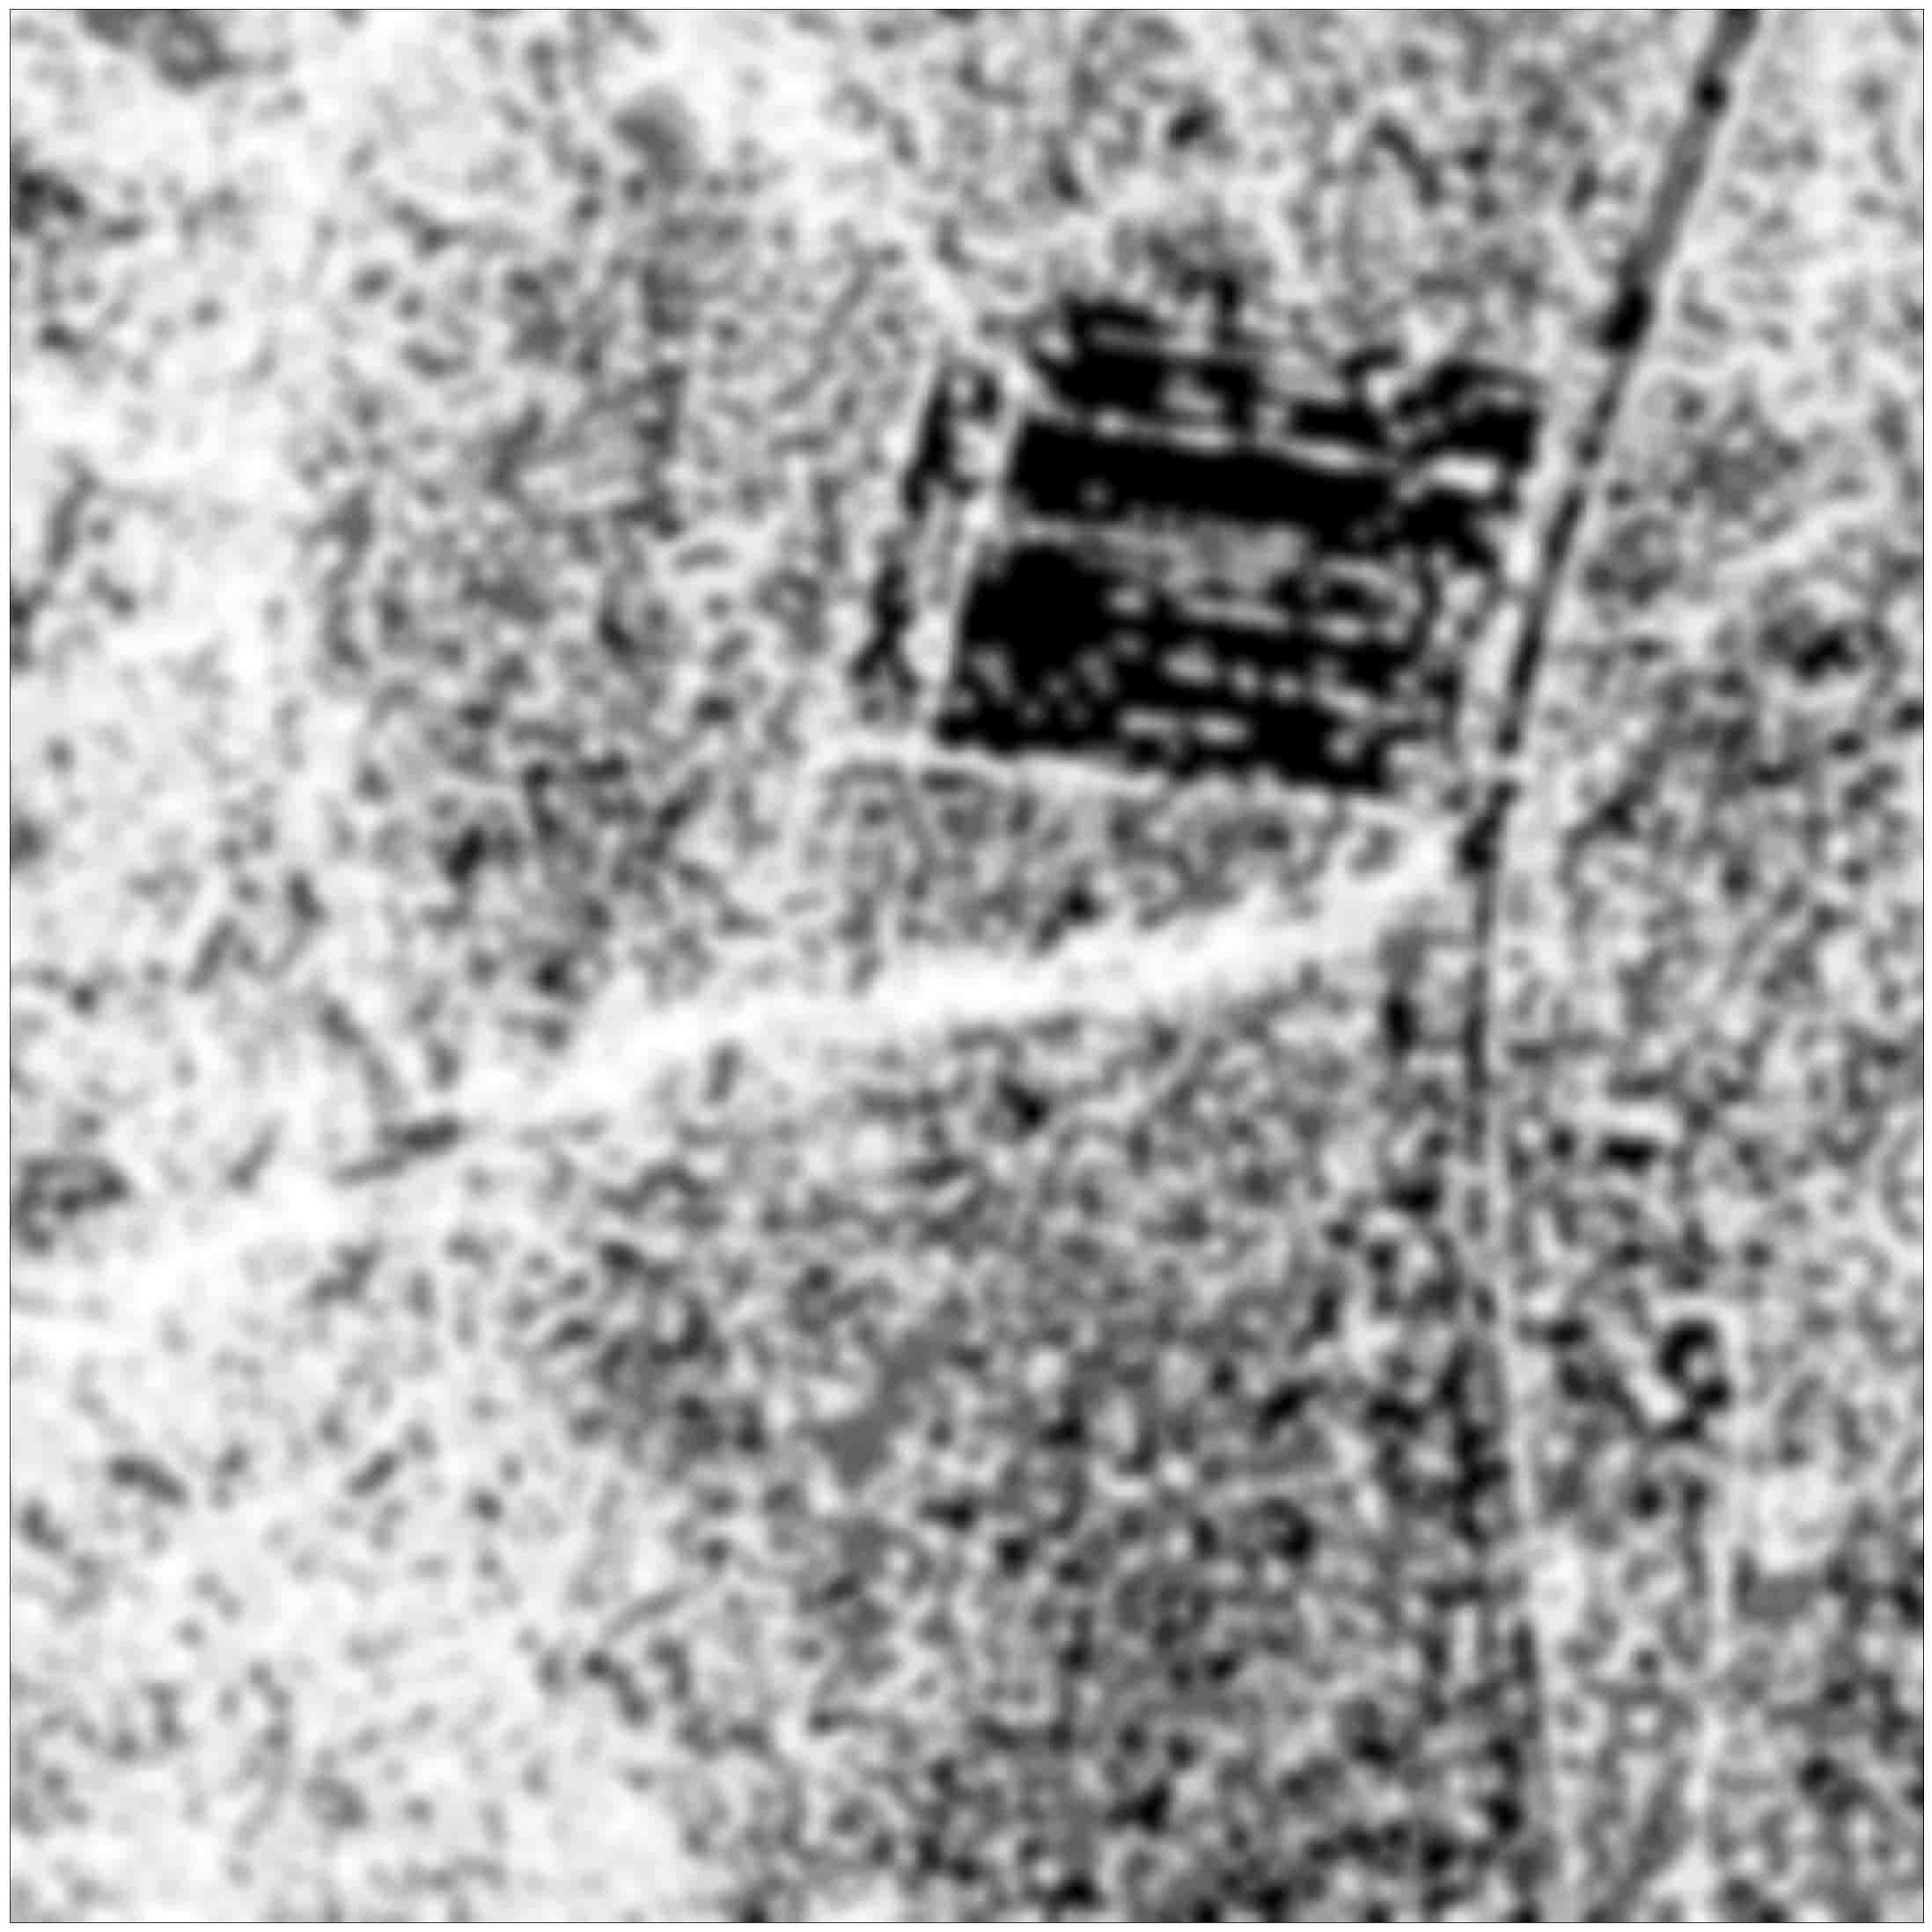
\includegraphics{./images/feature_d_lo.jpg}}}
%DIFDELCMD <     \subfigure[]{
%DIFDELCMD <         \resizebox*{4cm}{!}{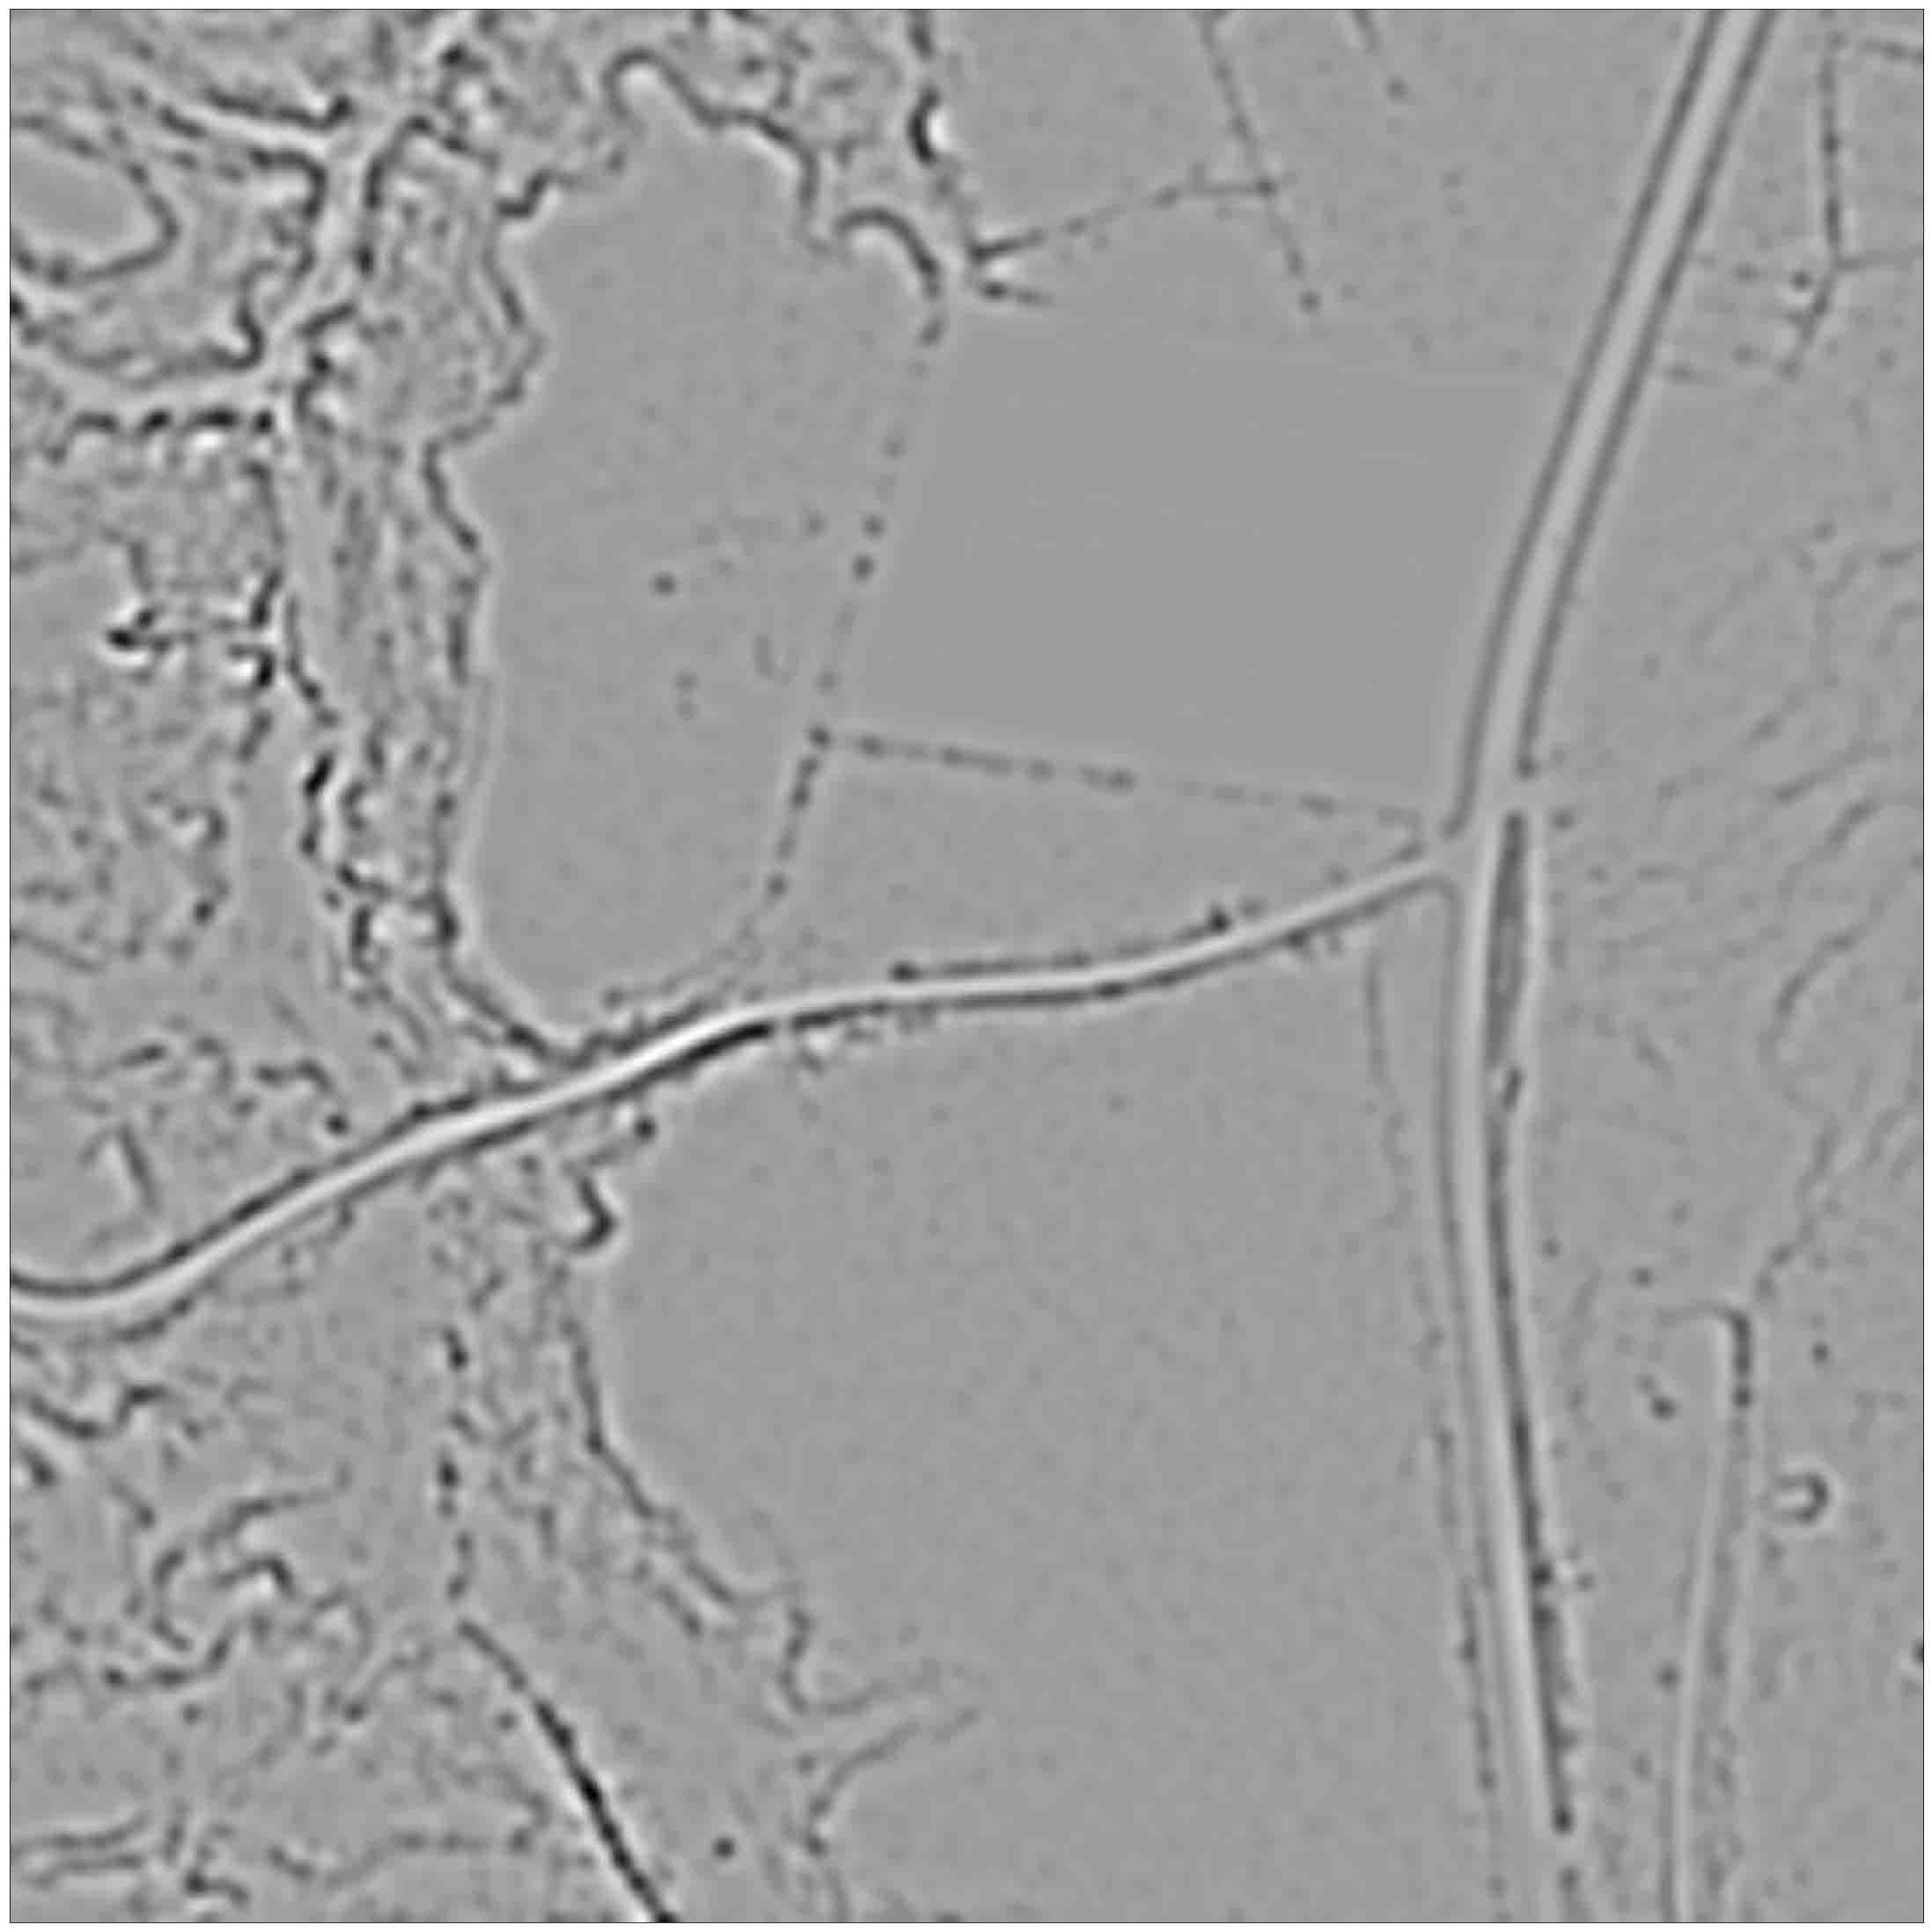
\includegraphics{./images/feature_e_lo.jpg}}}%%%
\DIFdelFL{\hspace{5pt}
    }%DIFDELCMD < \subfigure[]{
%DIFDELCMD <         \resizebox*{4cm}{!}{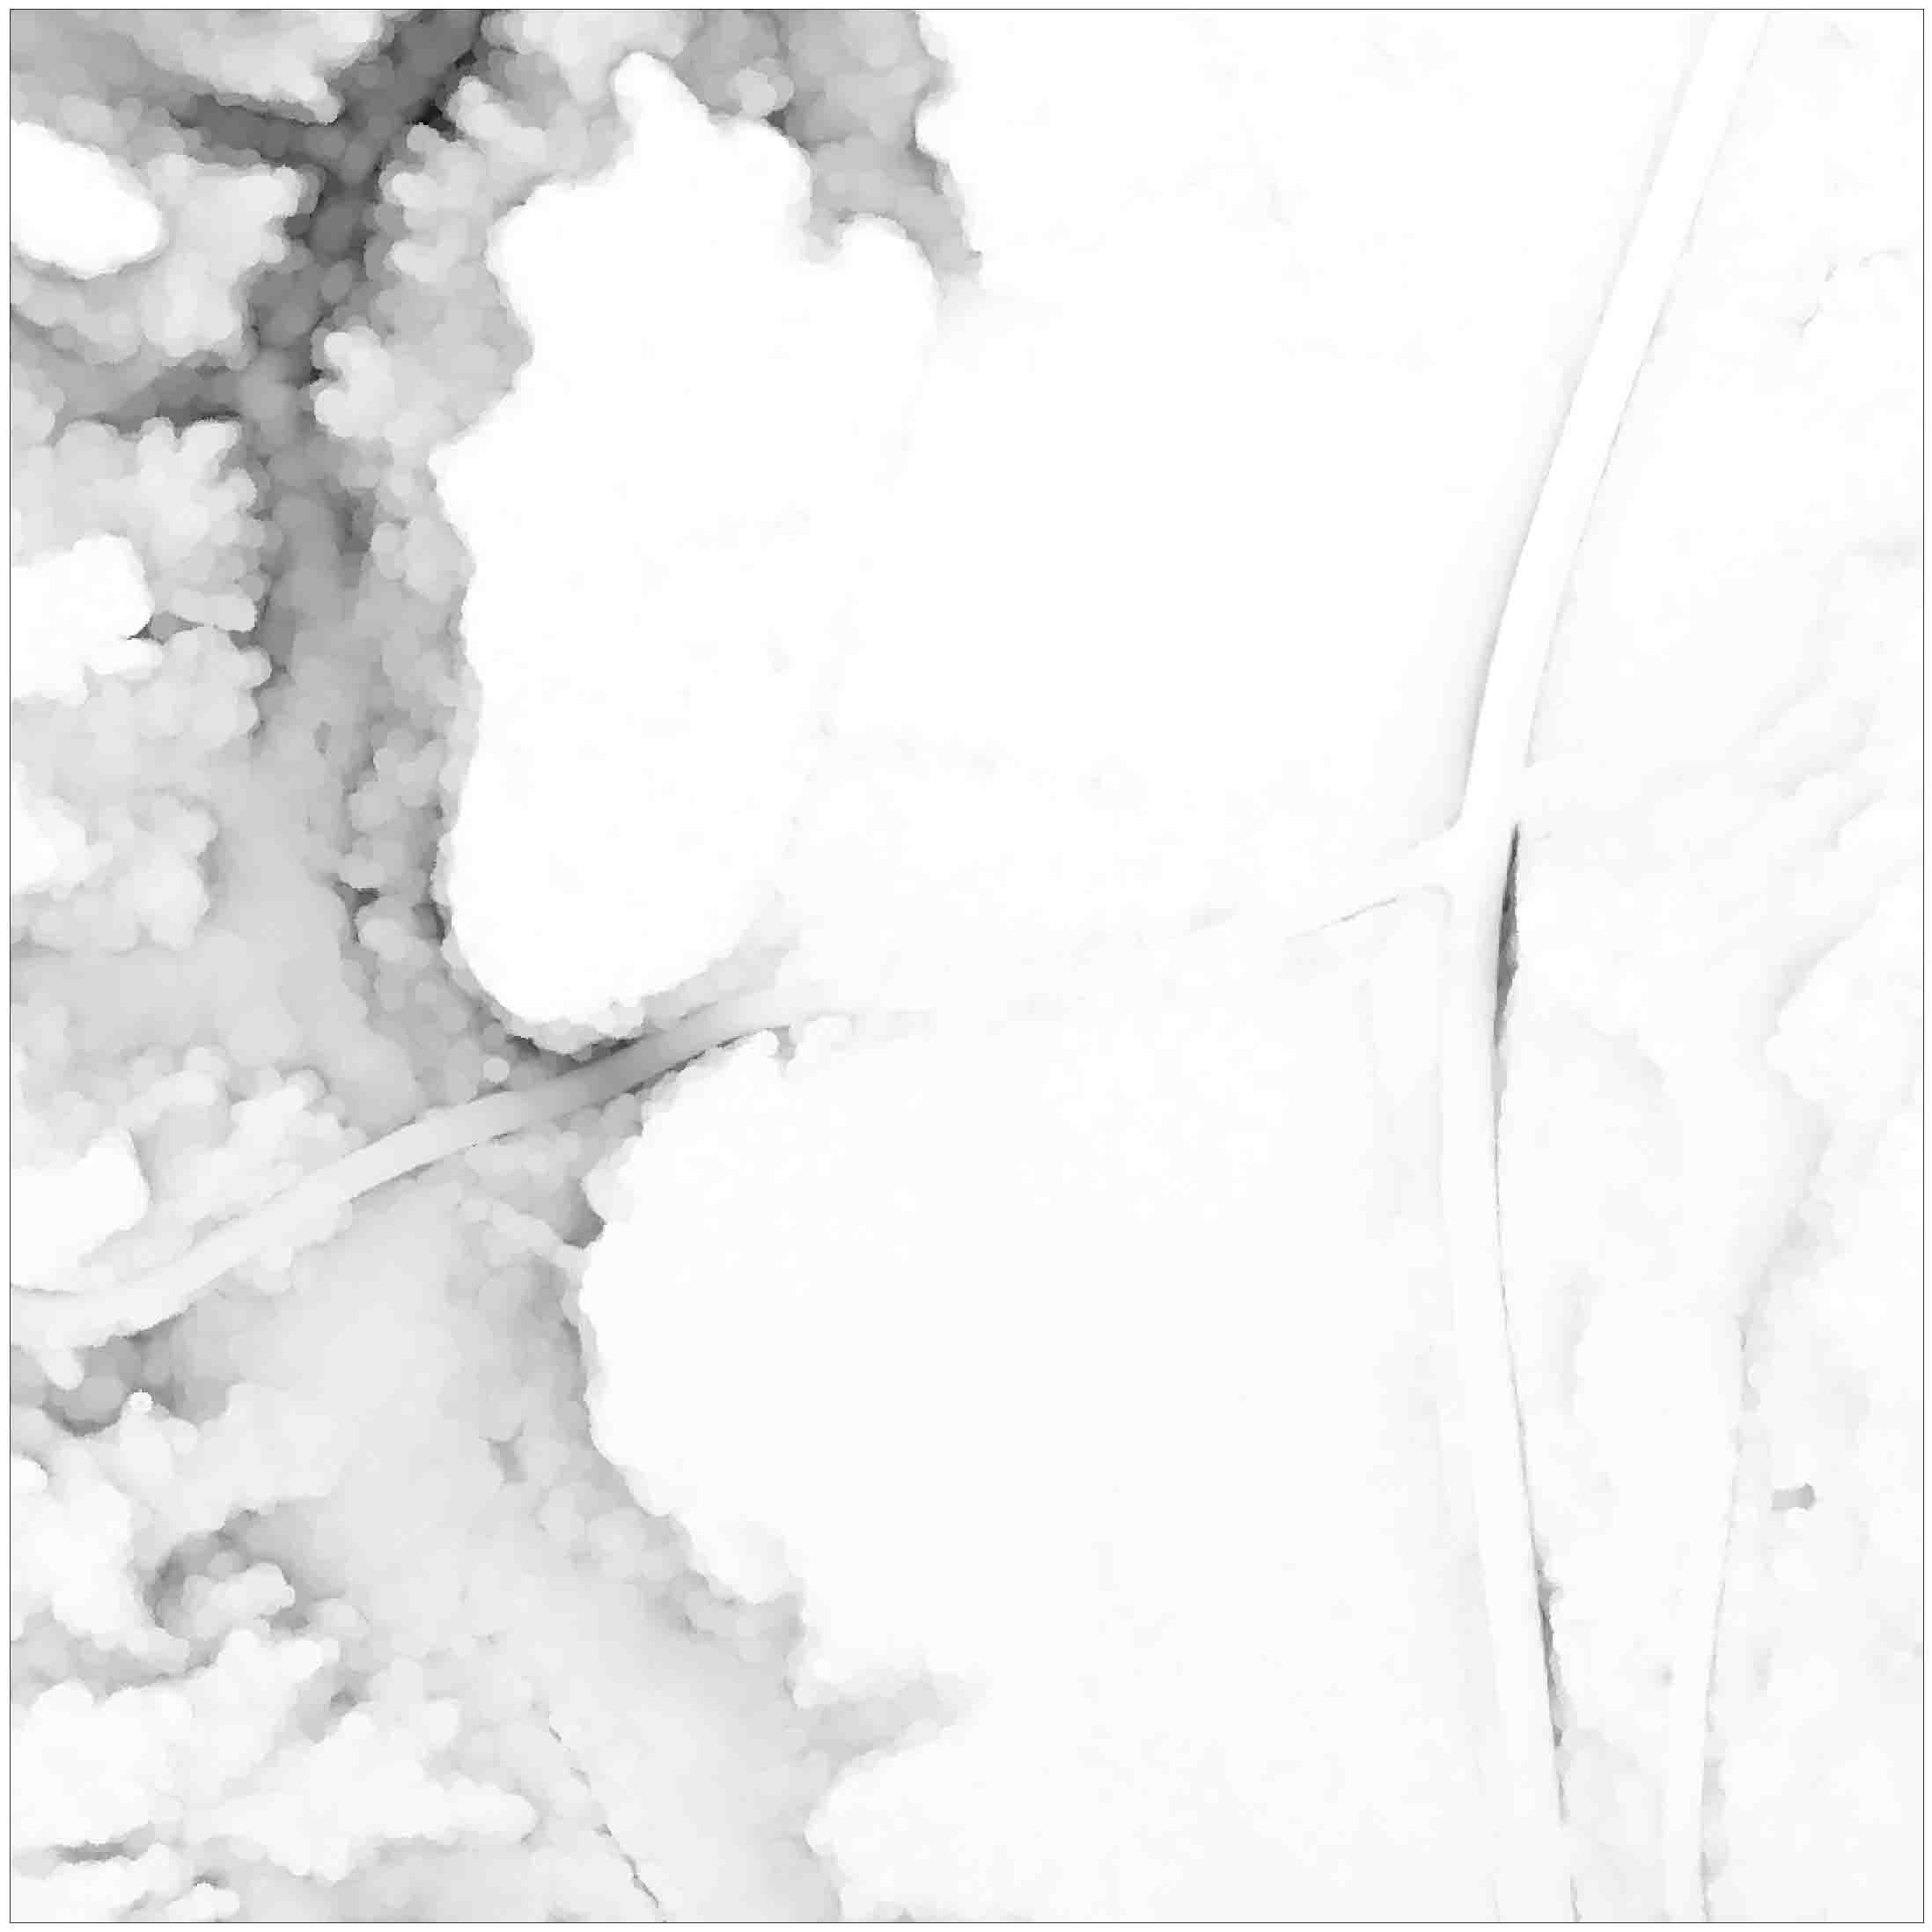
\includegraphics{./images/feature_f_lo.jpg}}}
%DIFDELCMD <     \subfigure[]{
%DIFDELCMD <         \resizebox*{4cm}{!}{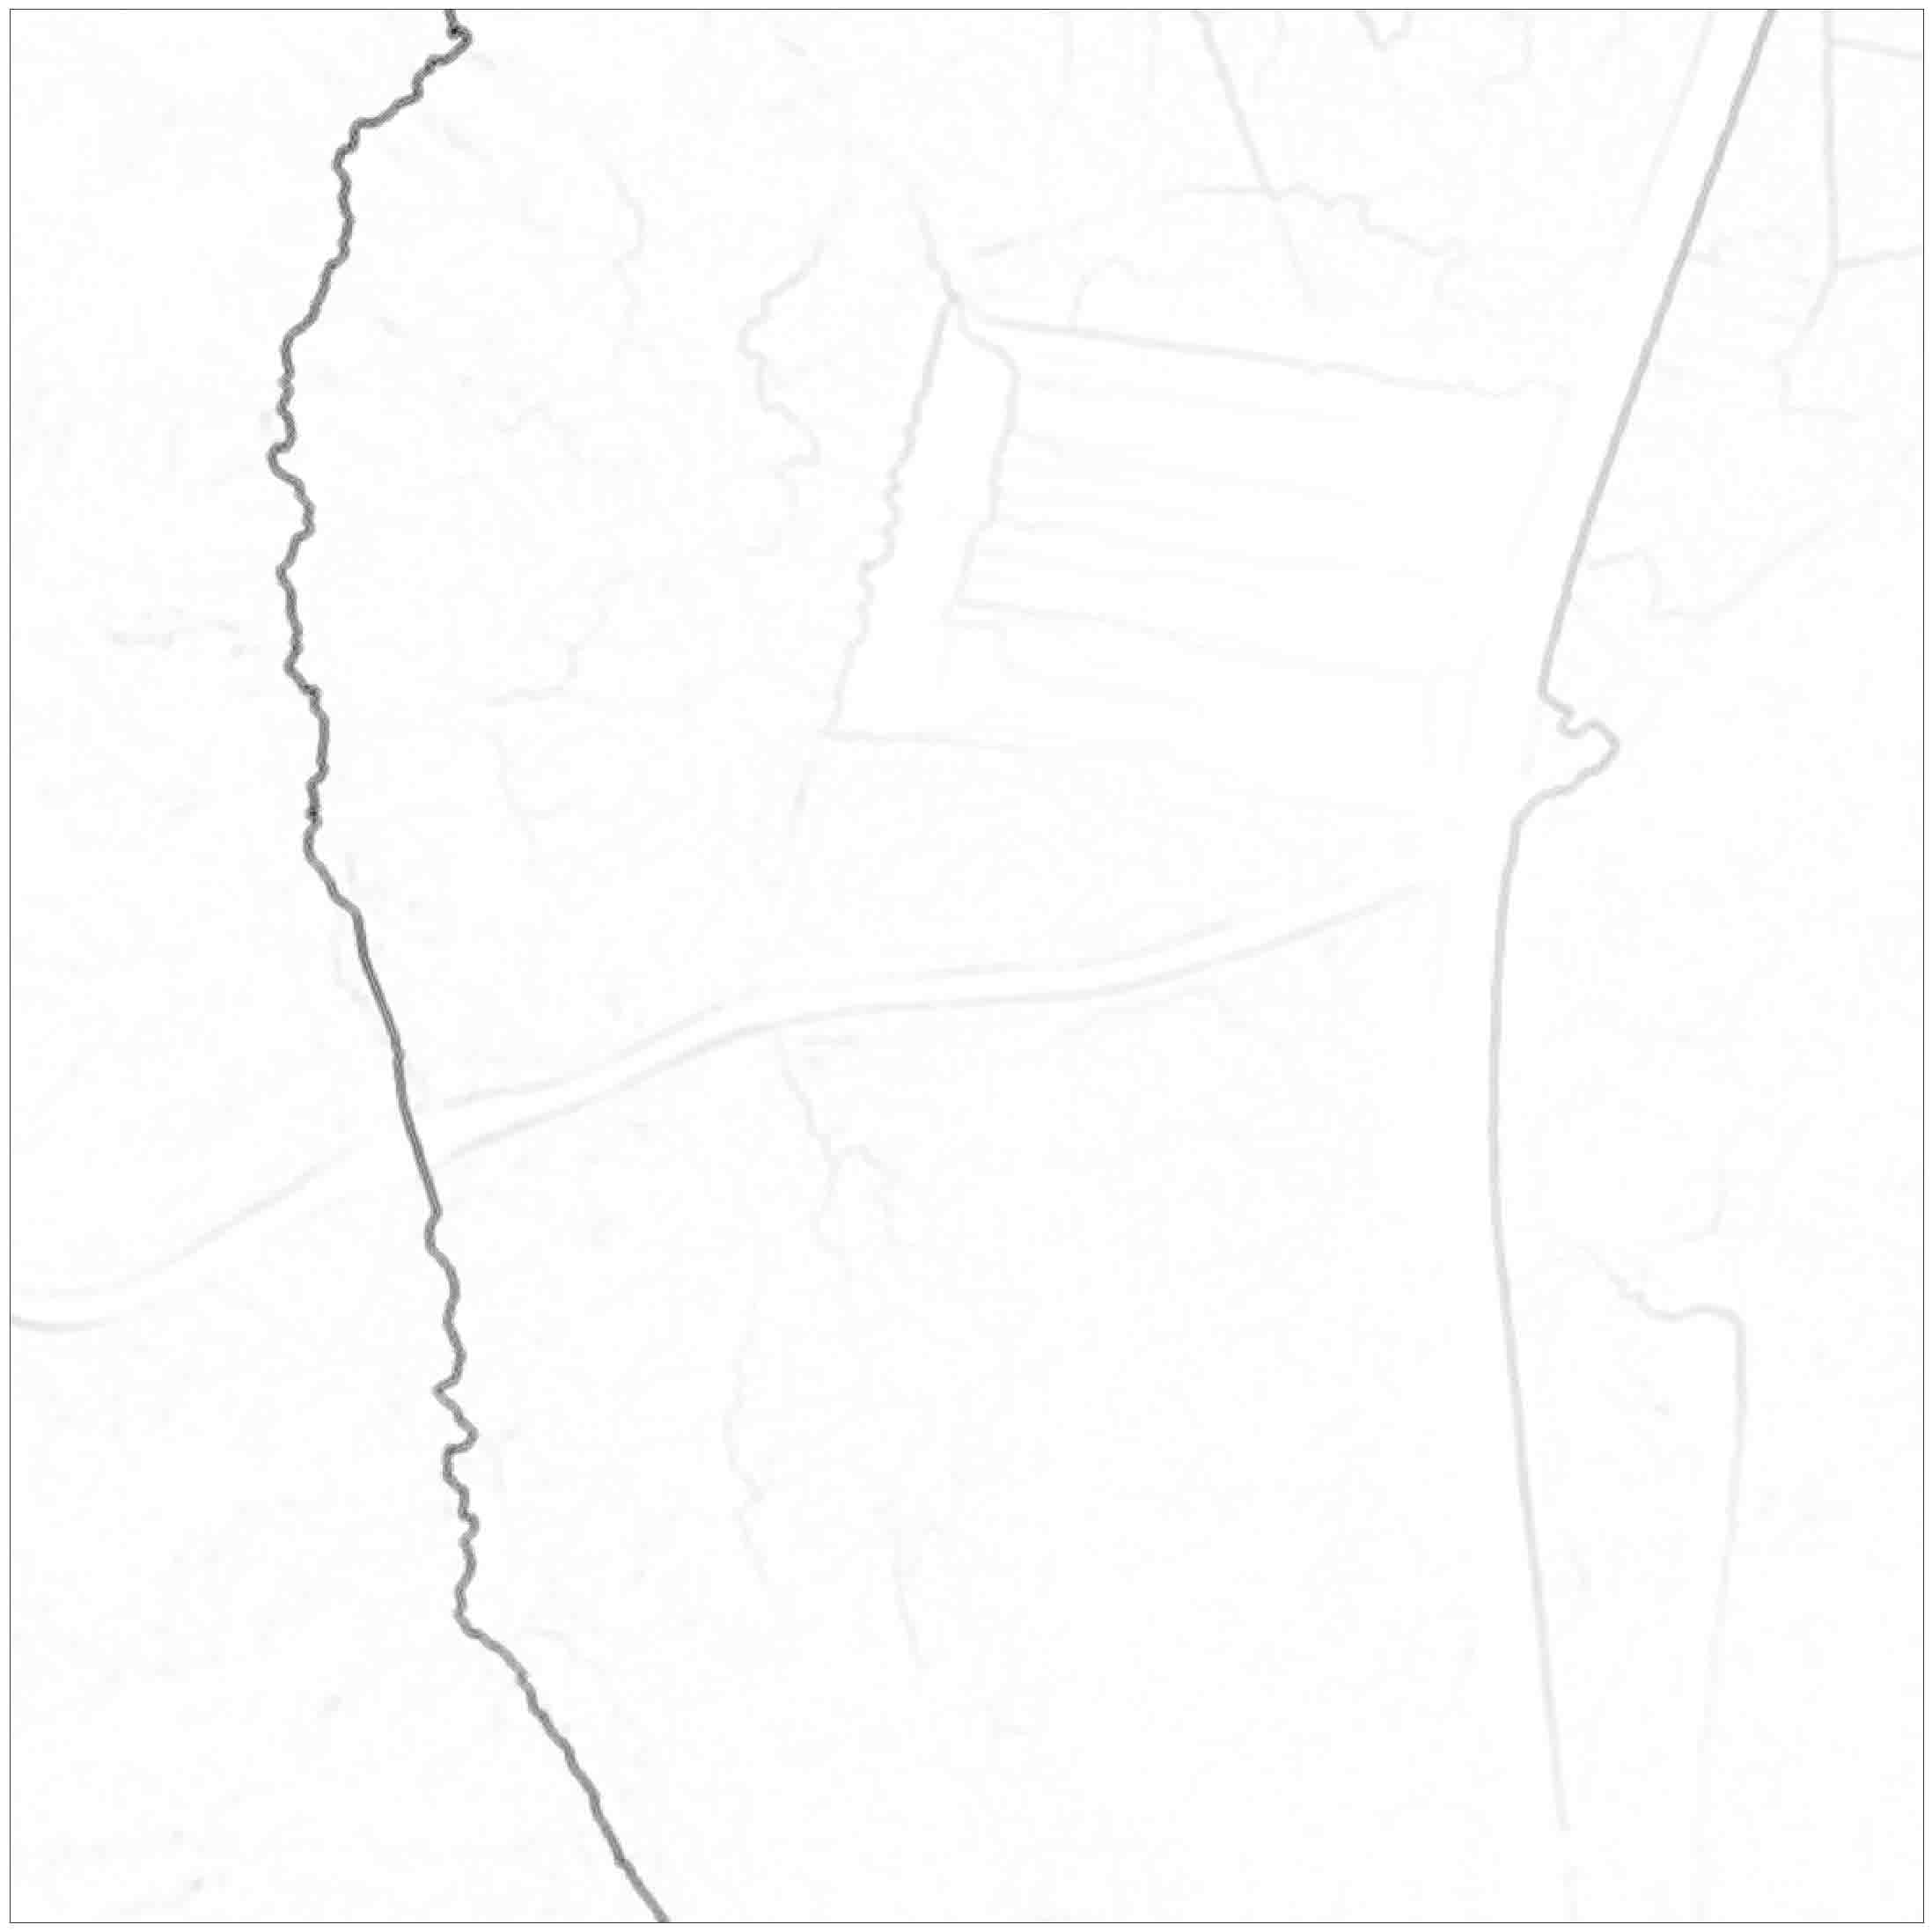
\includegraphics{./images/feature_g_lo.jpg}}}%%%
\DIFdelFL{\hspace{5pt}
    }%DIFDELCMD < \subfigure[]{
%DIFDELCMD <         \resizebox*{4cm}{!}{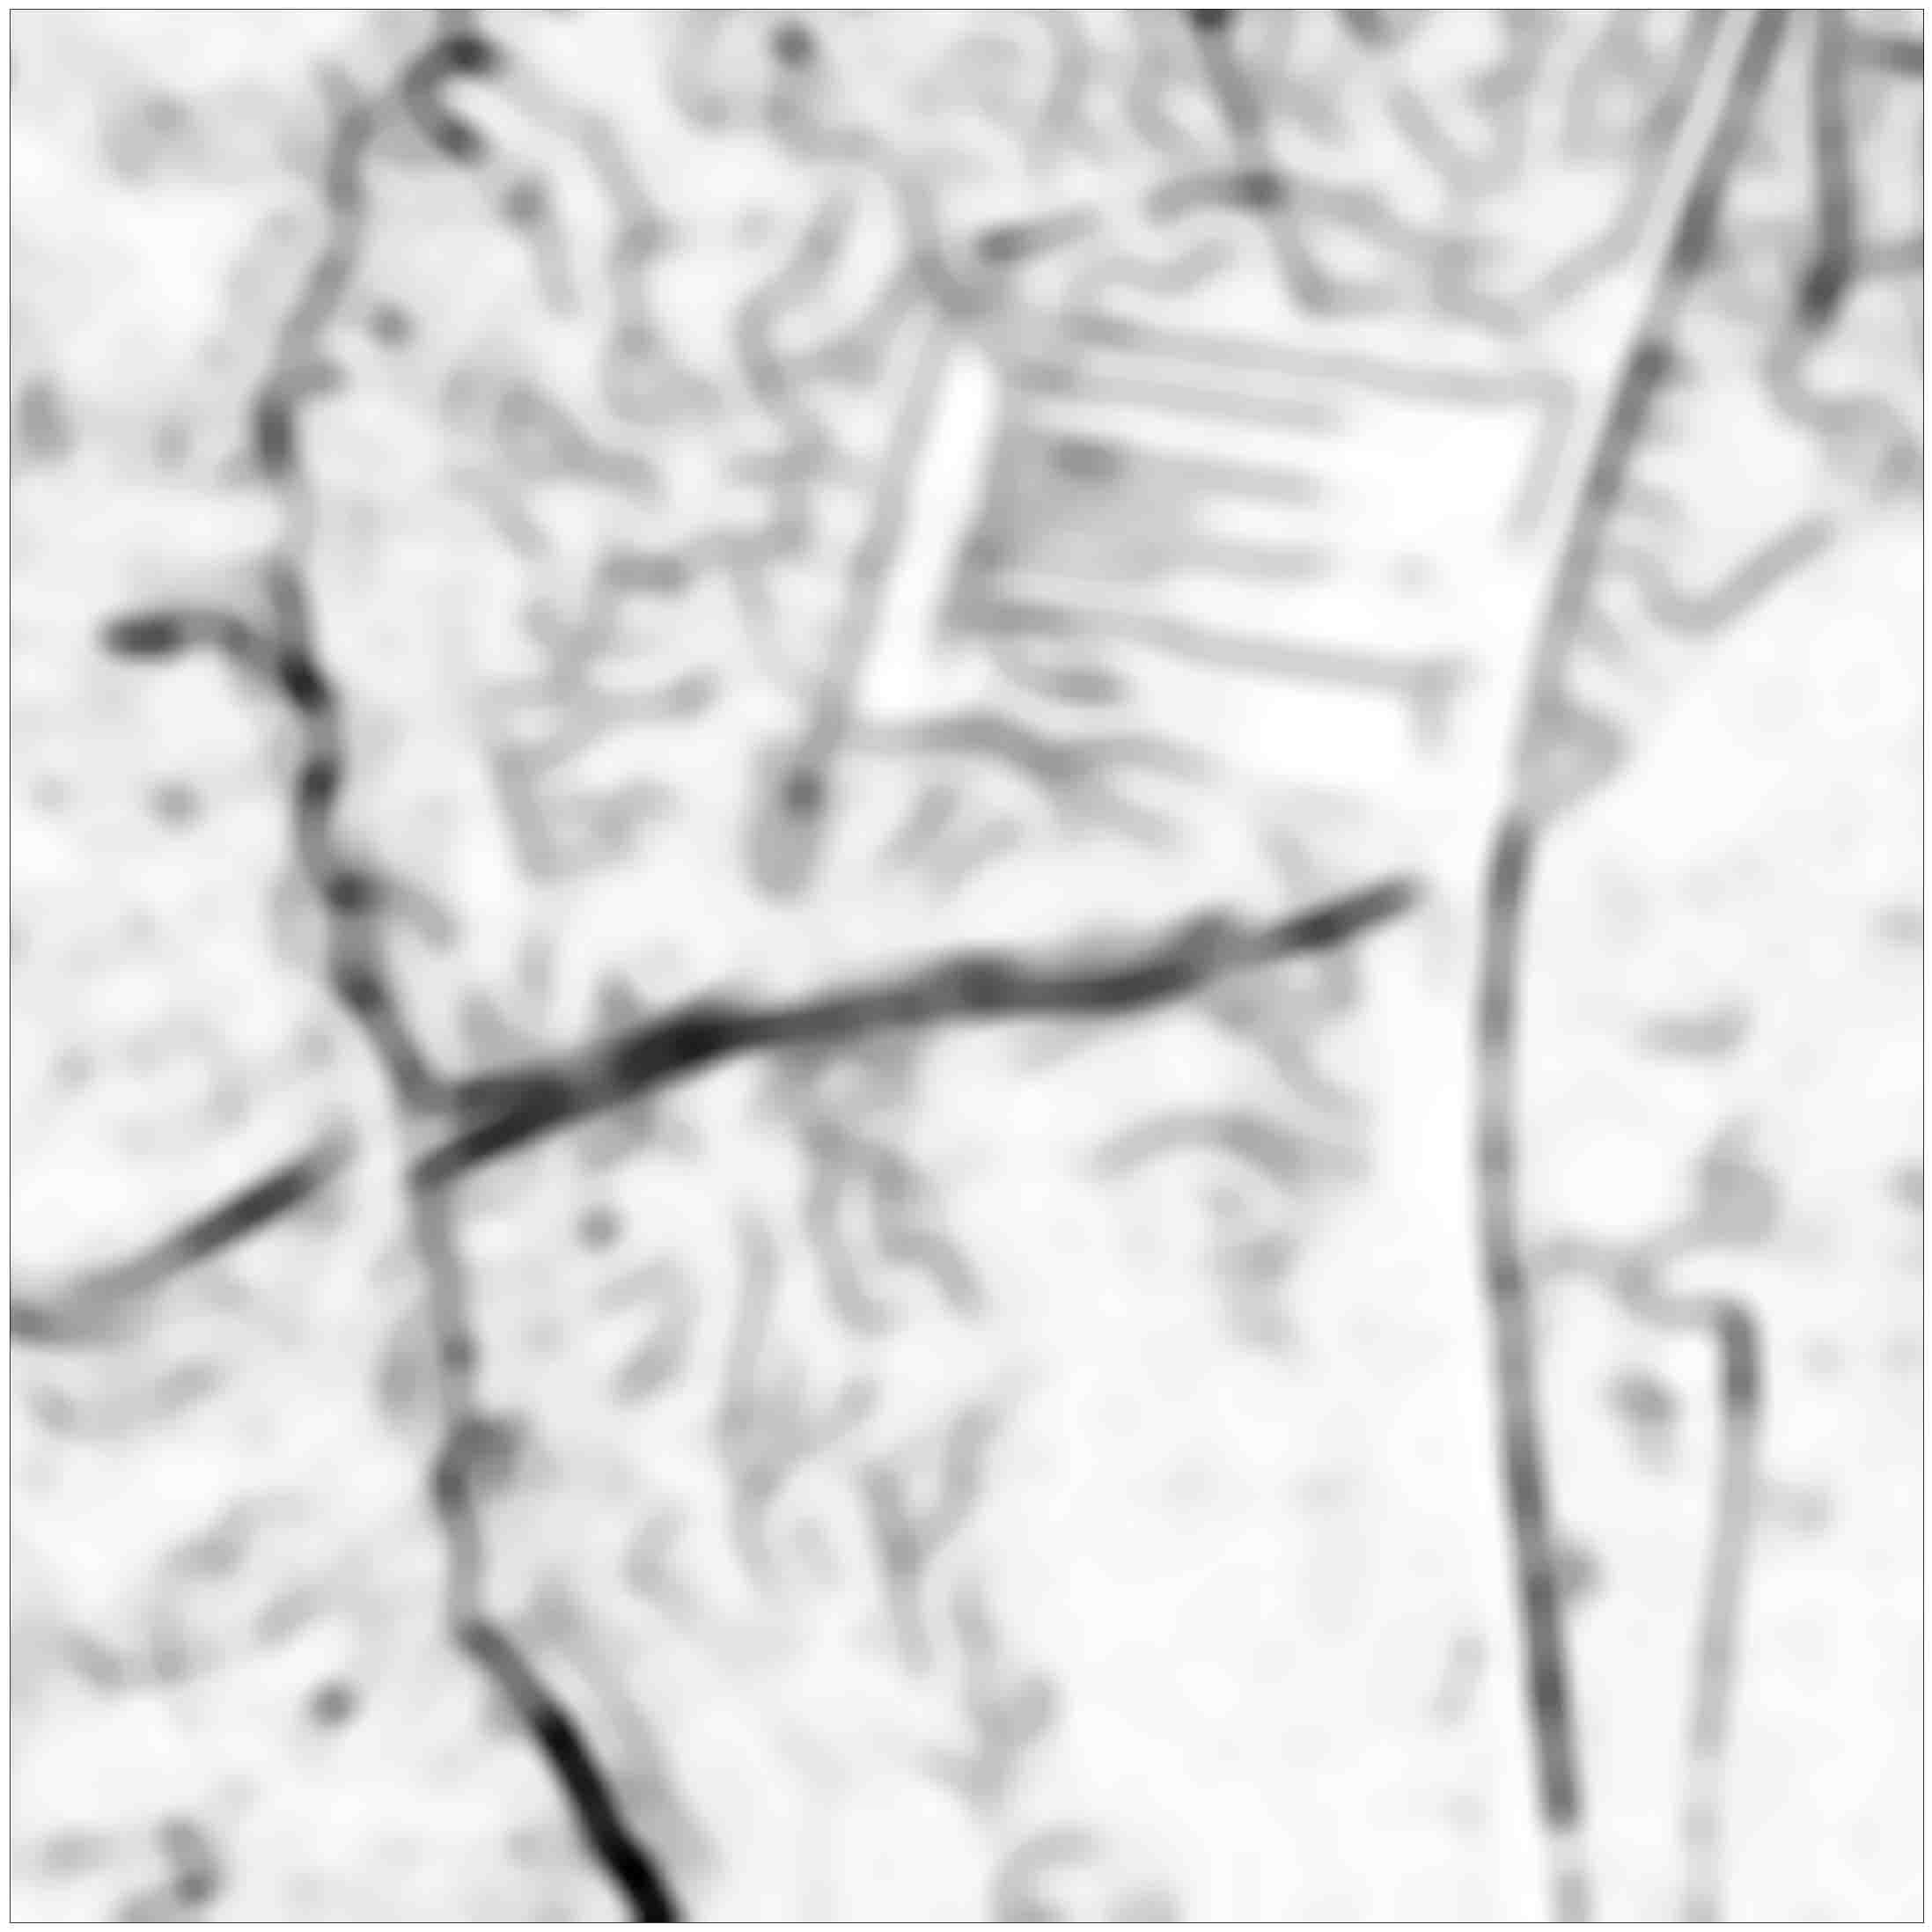
\includegraphics{./images/feature_h_lo.jpg}}}
%DIFDELCMD <     \subfigure[]{
%DIFDELCMD <         \resizebox*{4cm}{!}{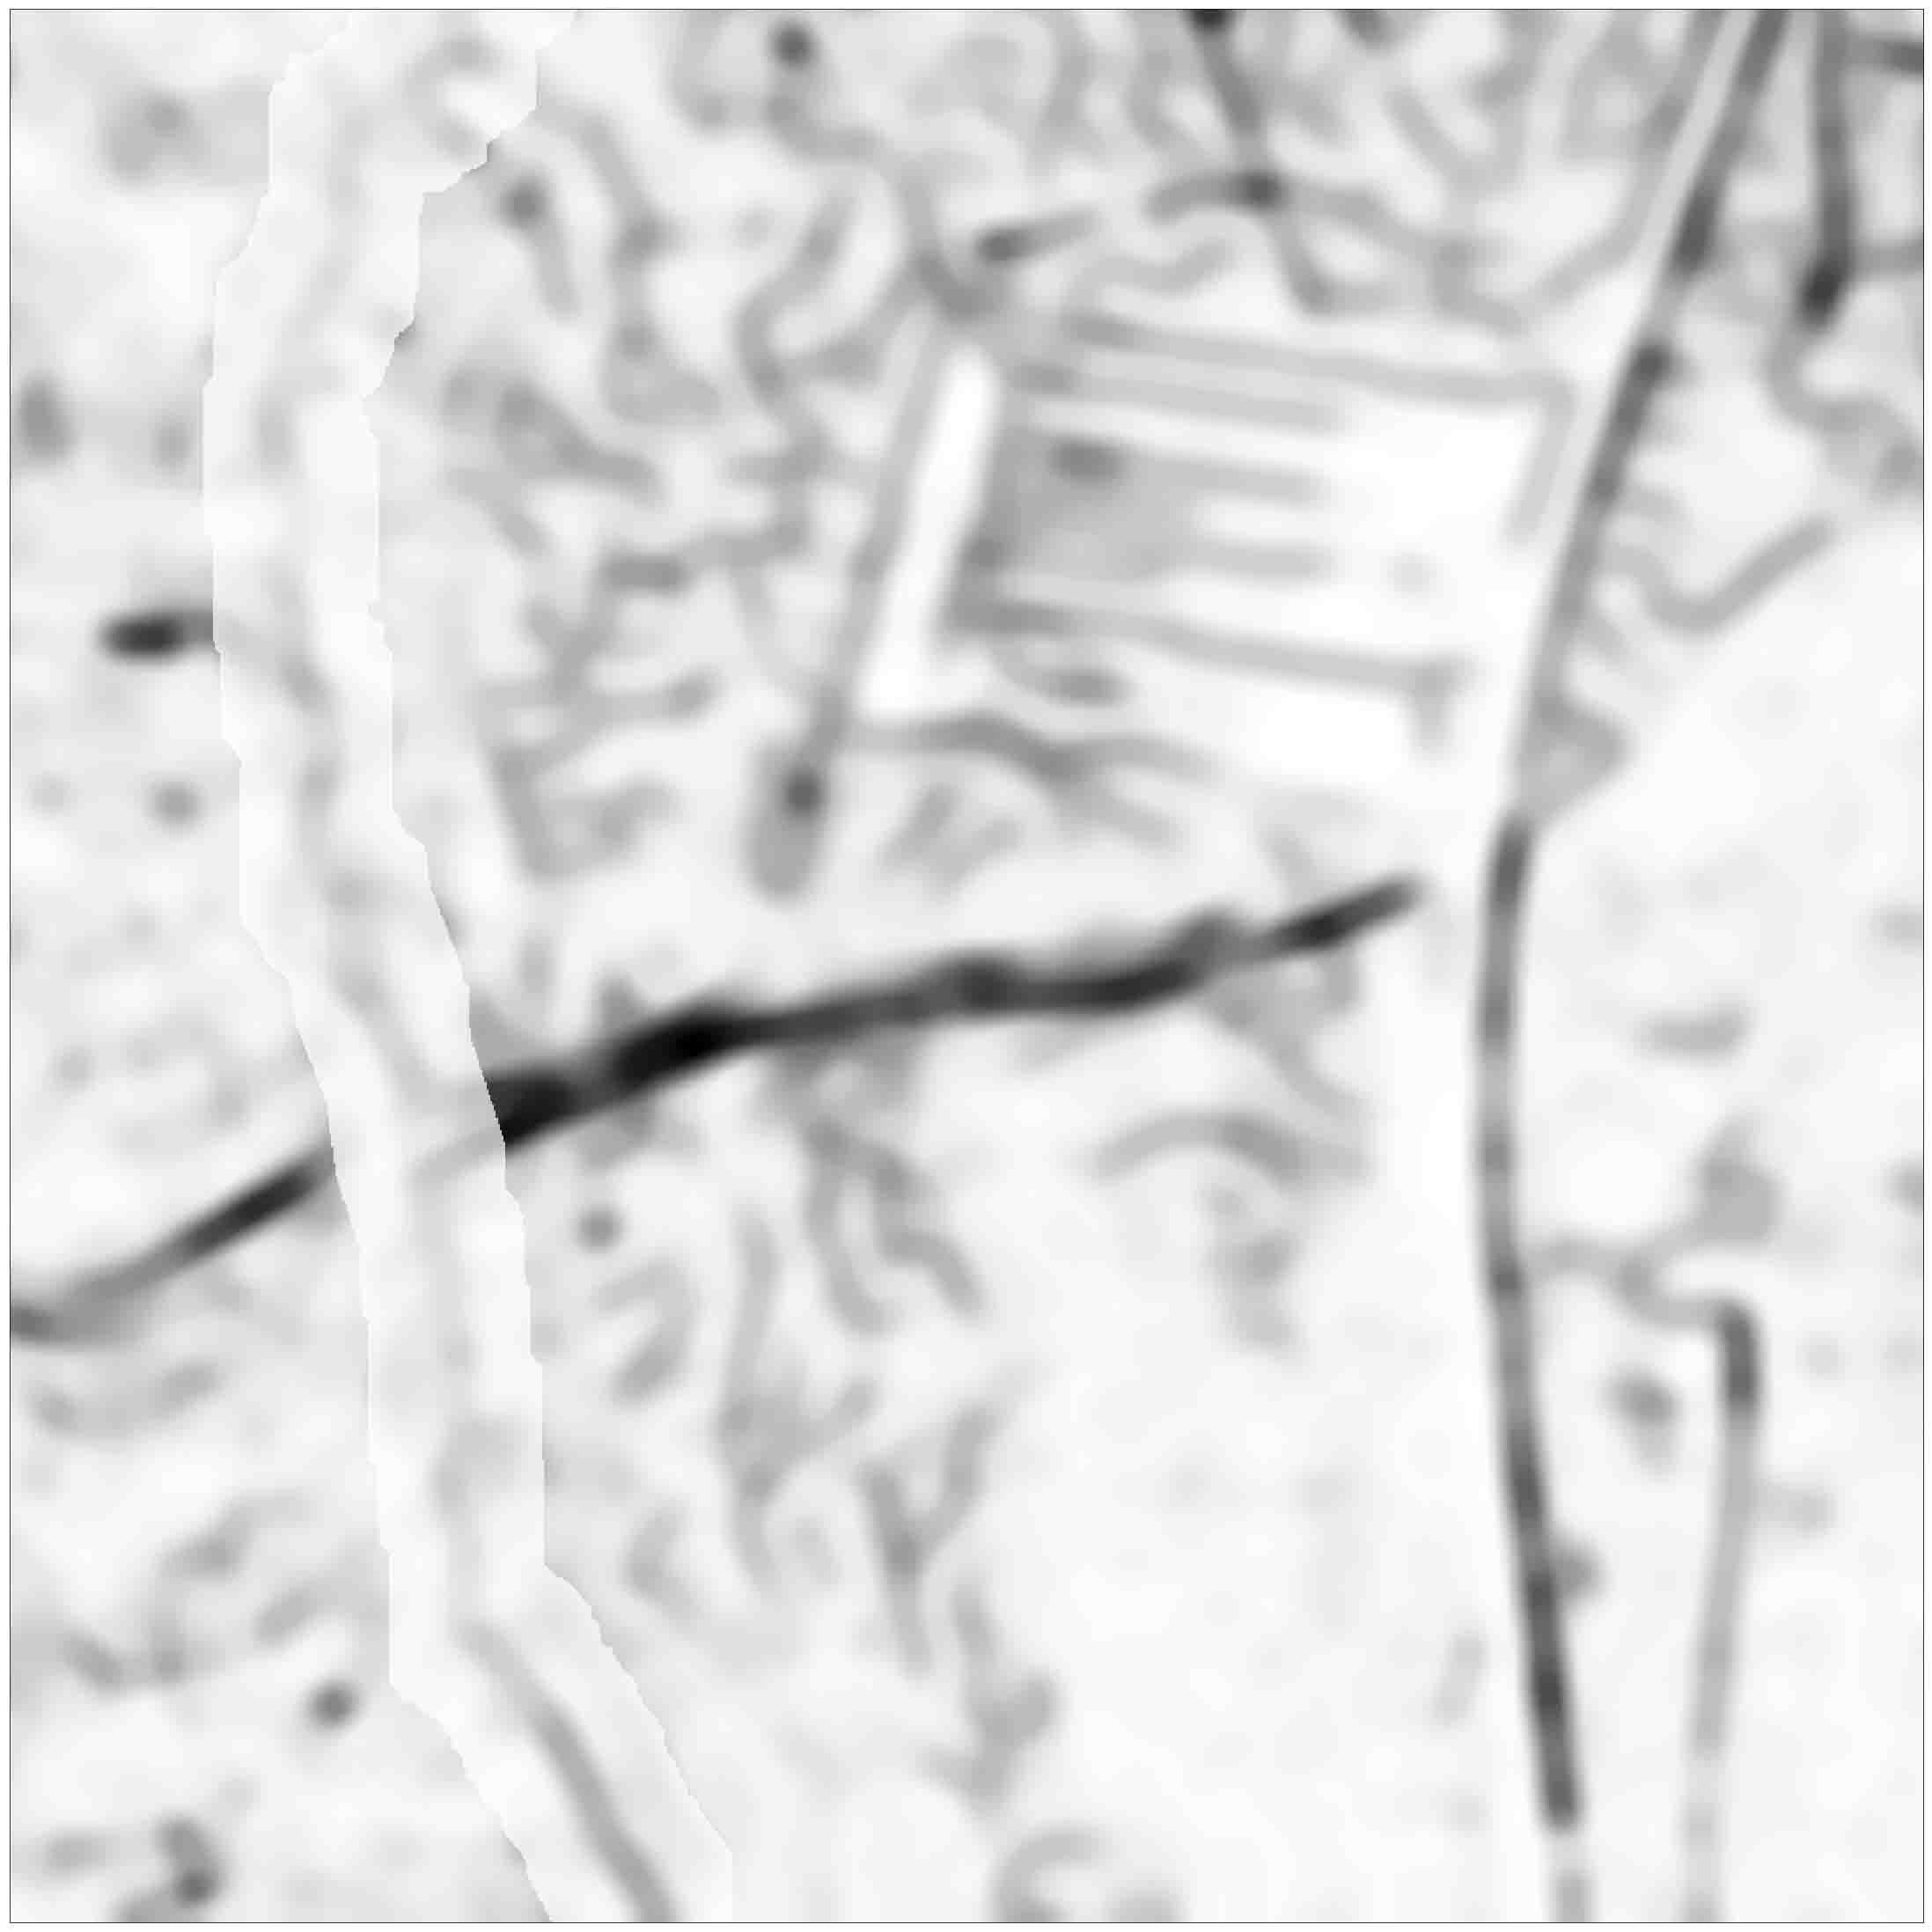
\includegraphics{./images/feature_i_lo.jpg}}}
%DIFDELCMD <     %%%
\DIFdelendFL \DIFaddbeginFL \subfigure[]{
        \resizebox*{3.5cm}{!}{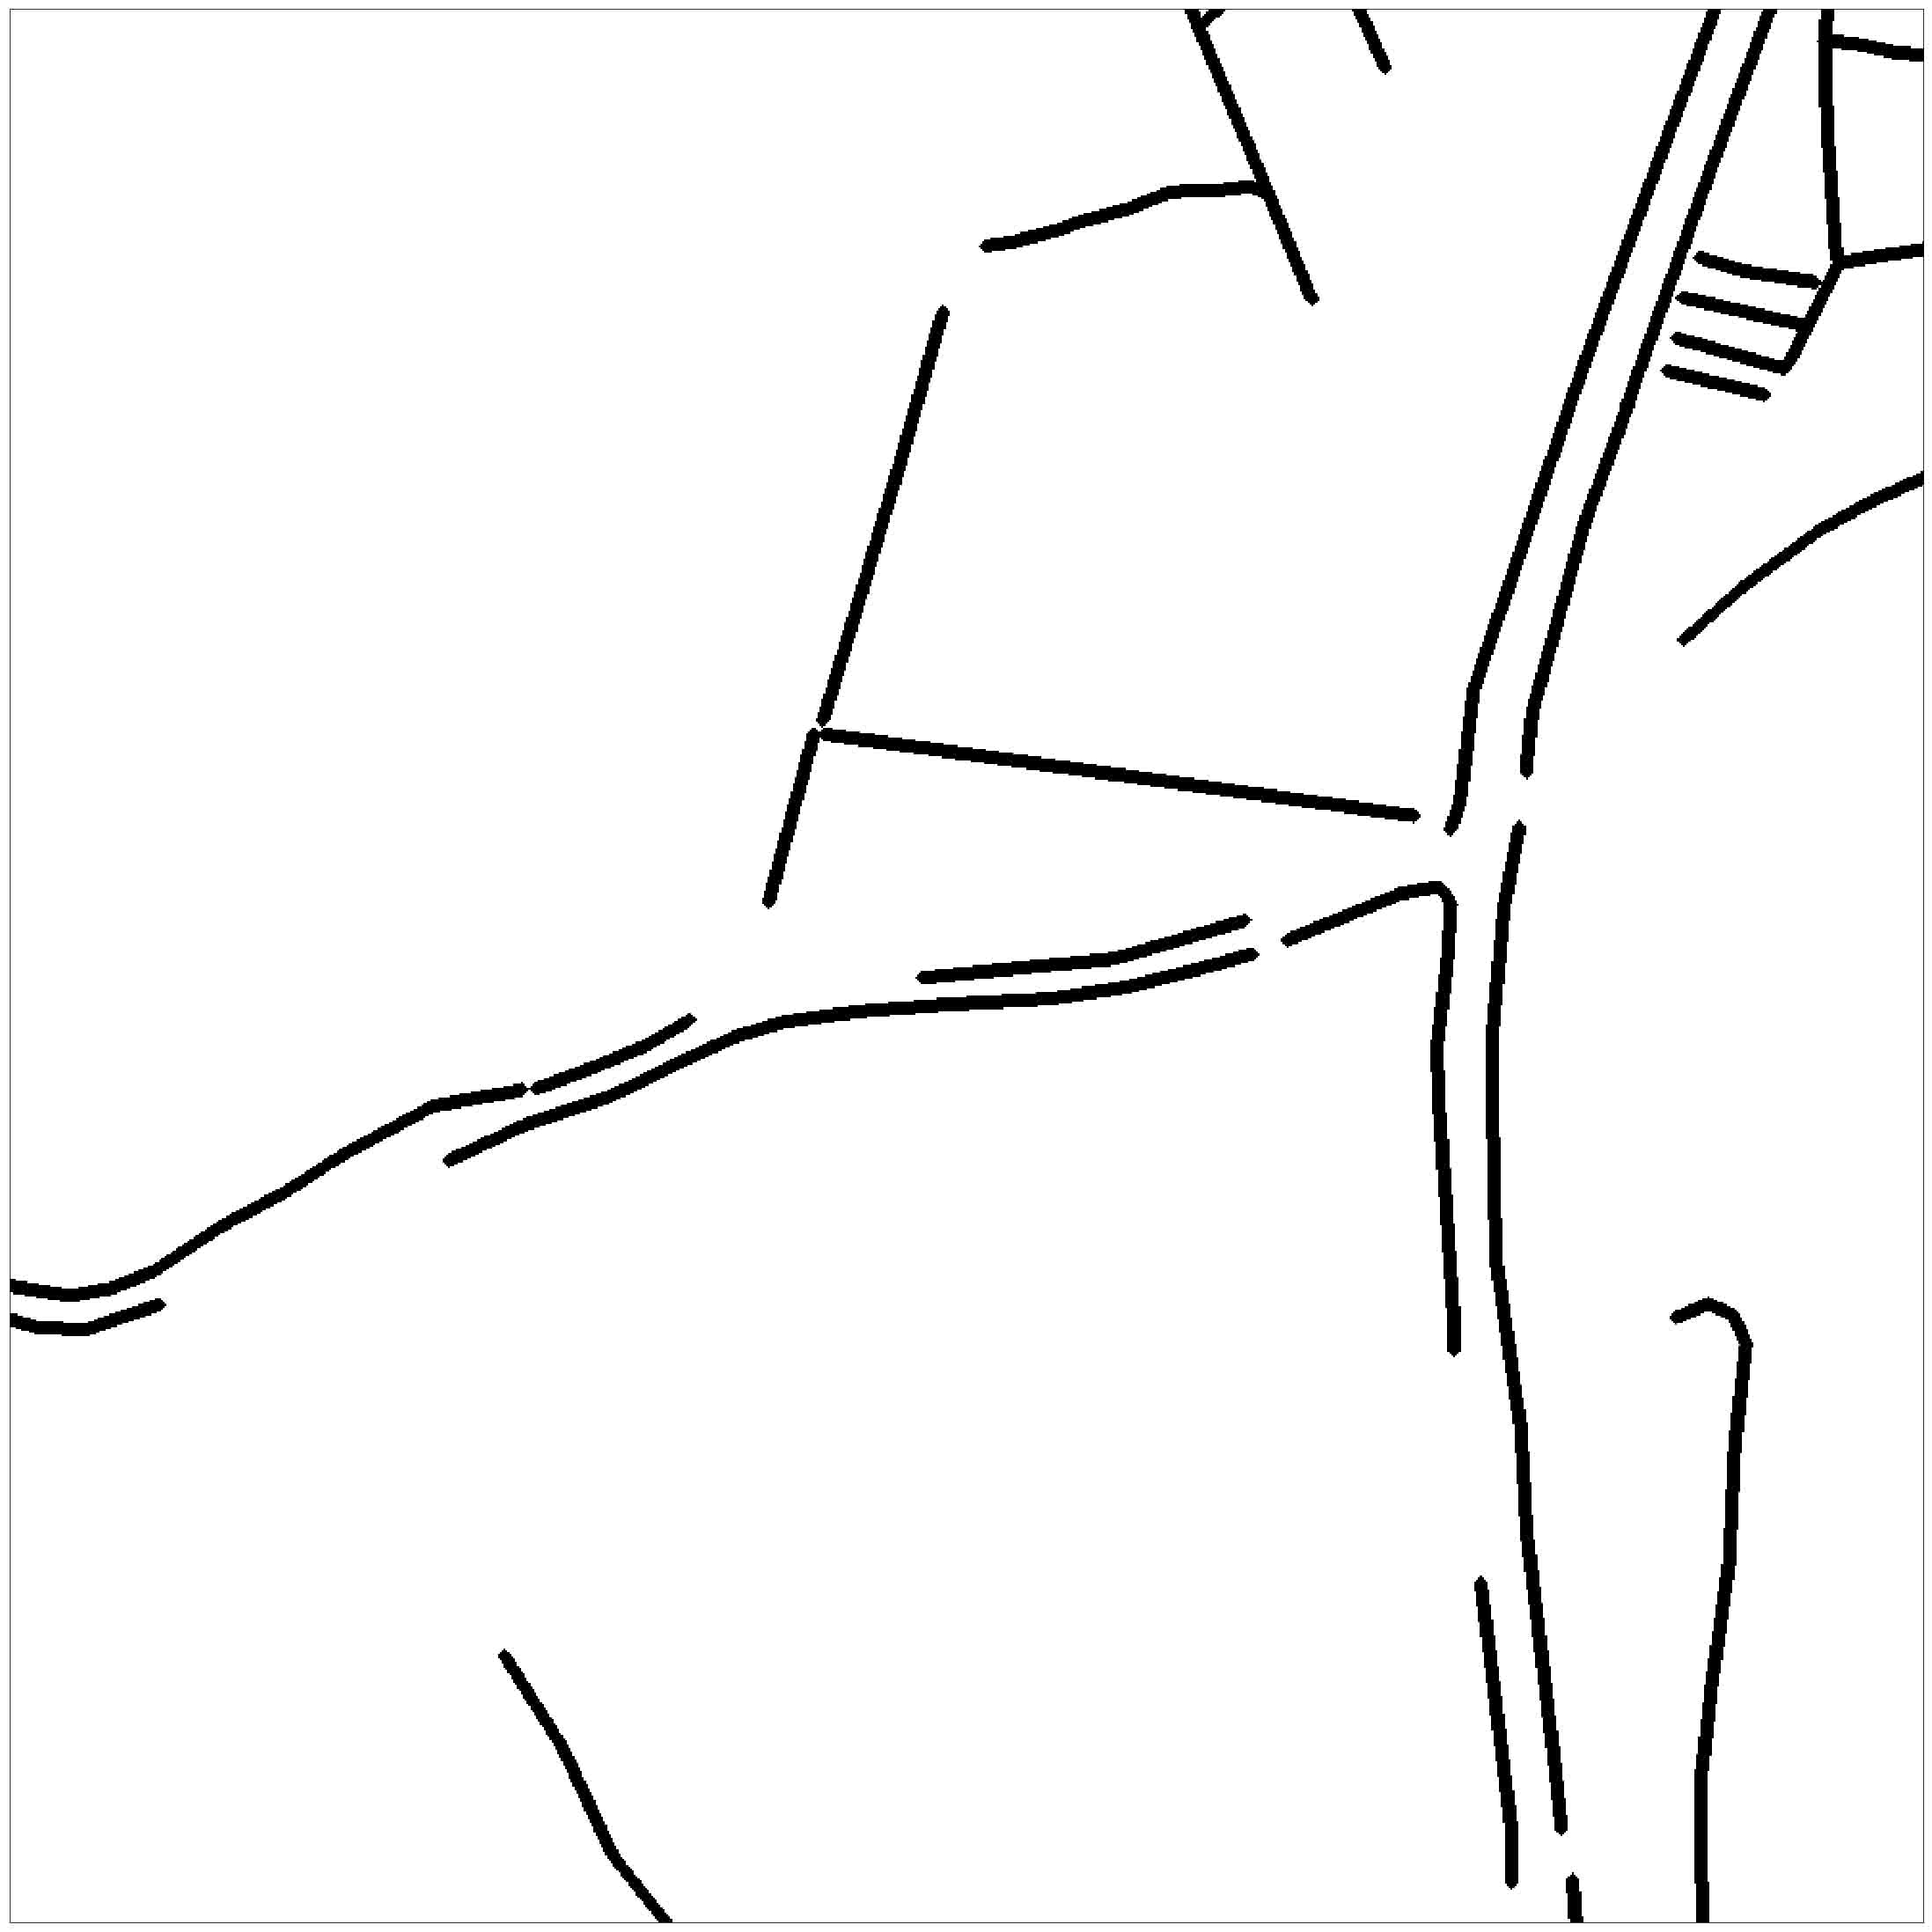
\includegraphics{./images/feature_a_lo.jpg}}}
    \subfigure[]{
        \resizebox*{3.5cm}{!}{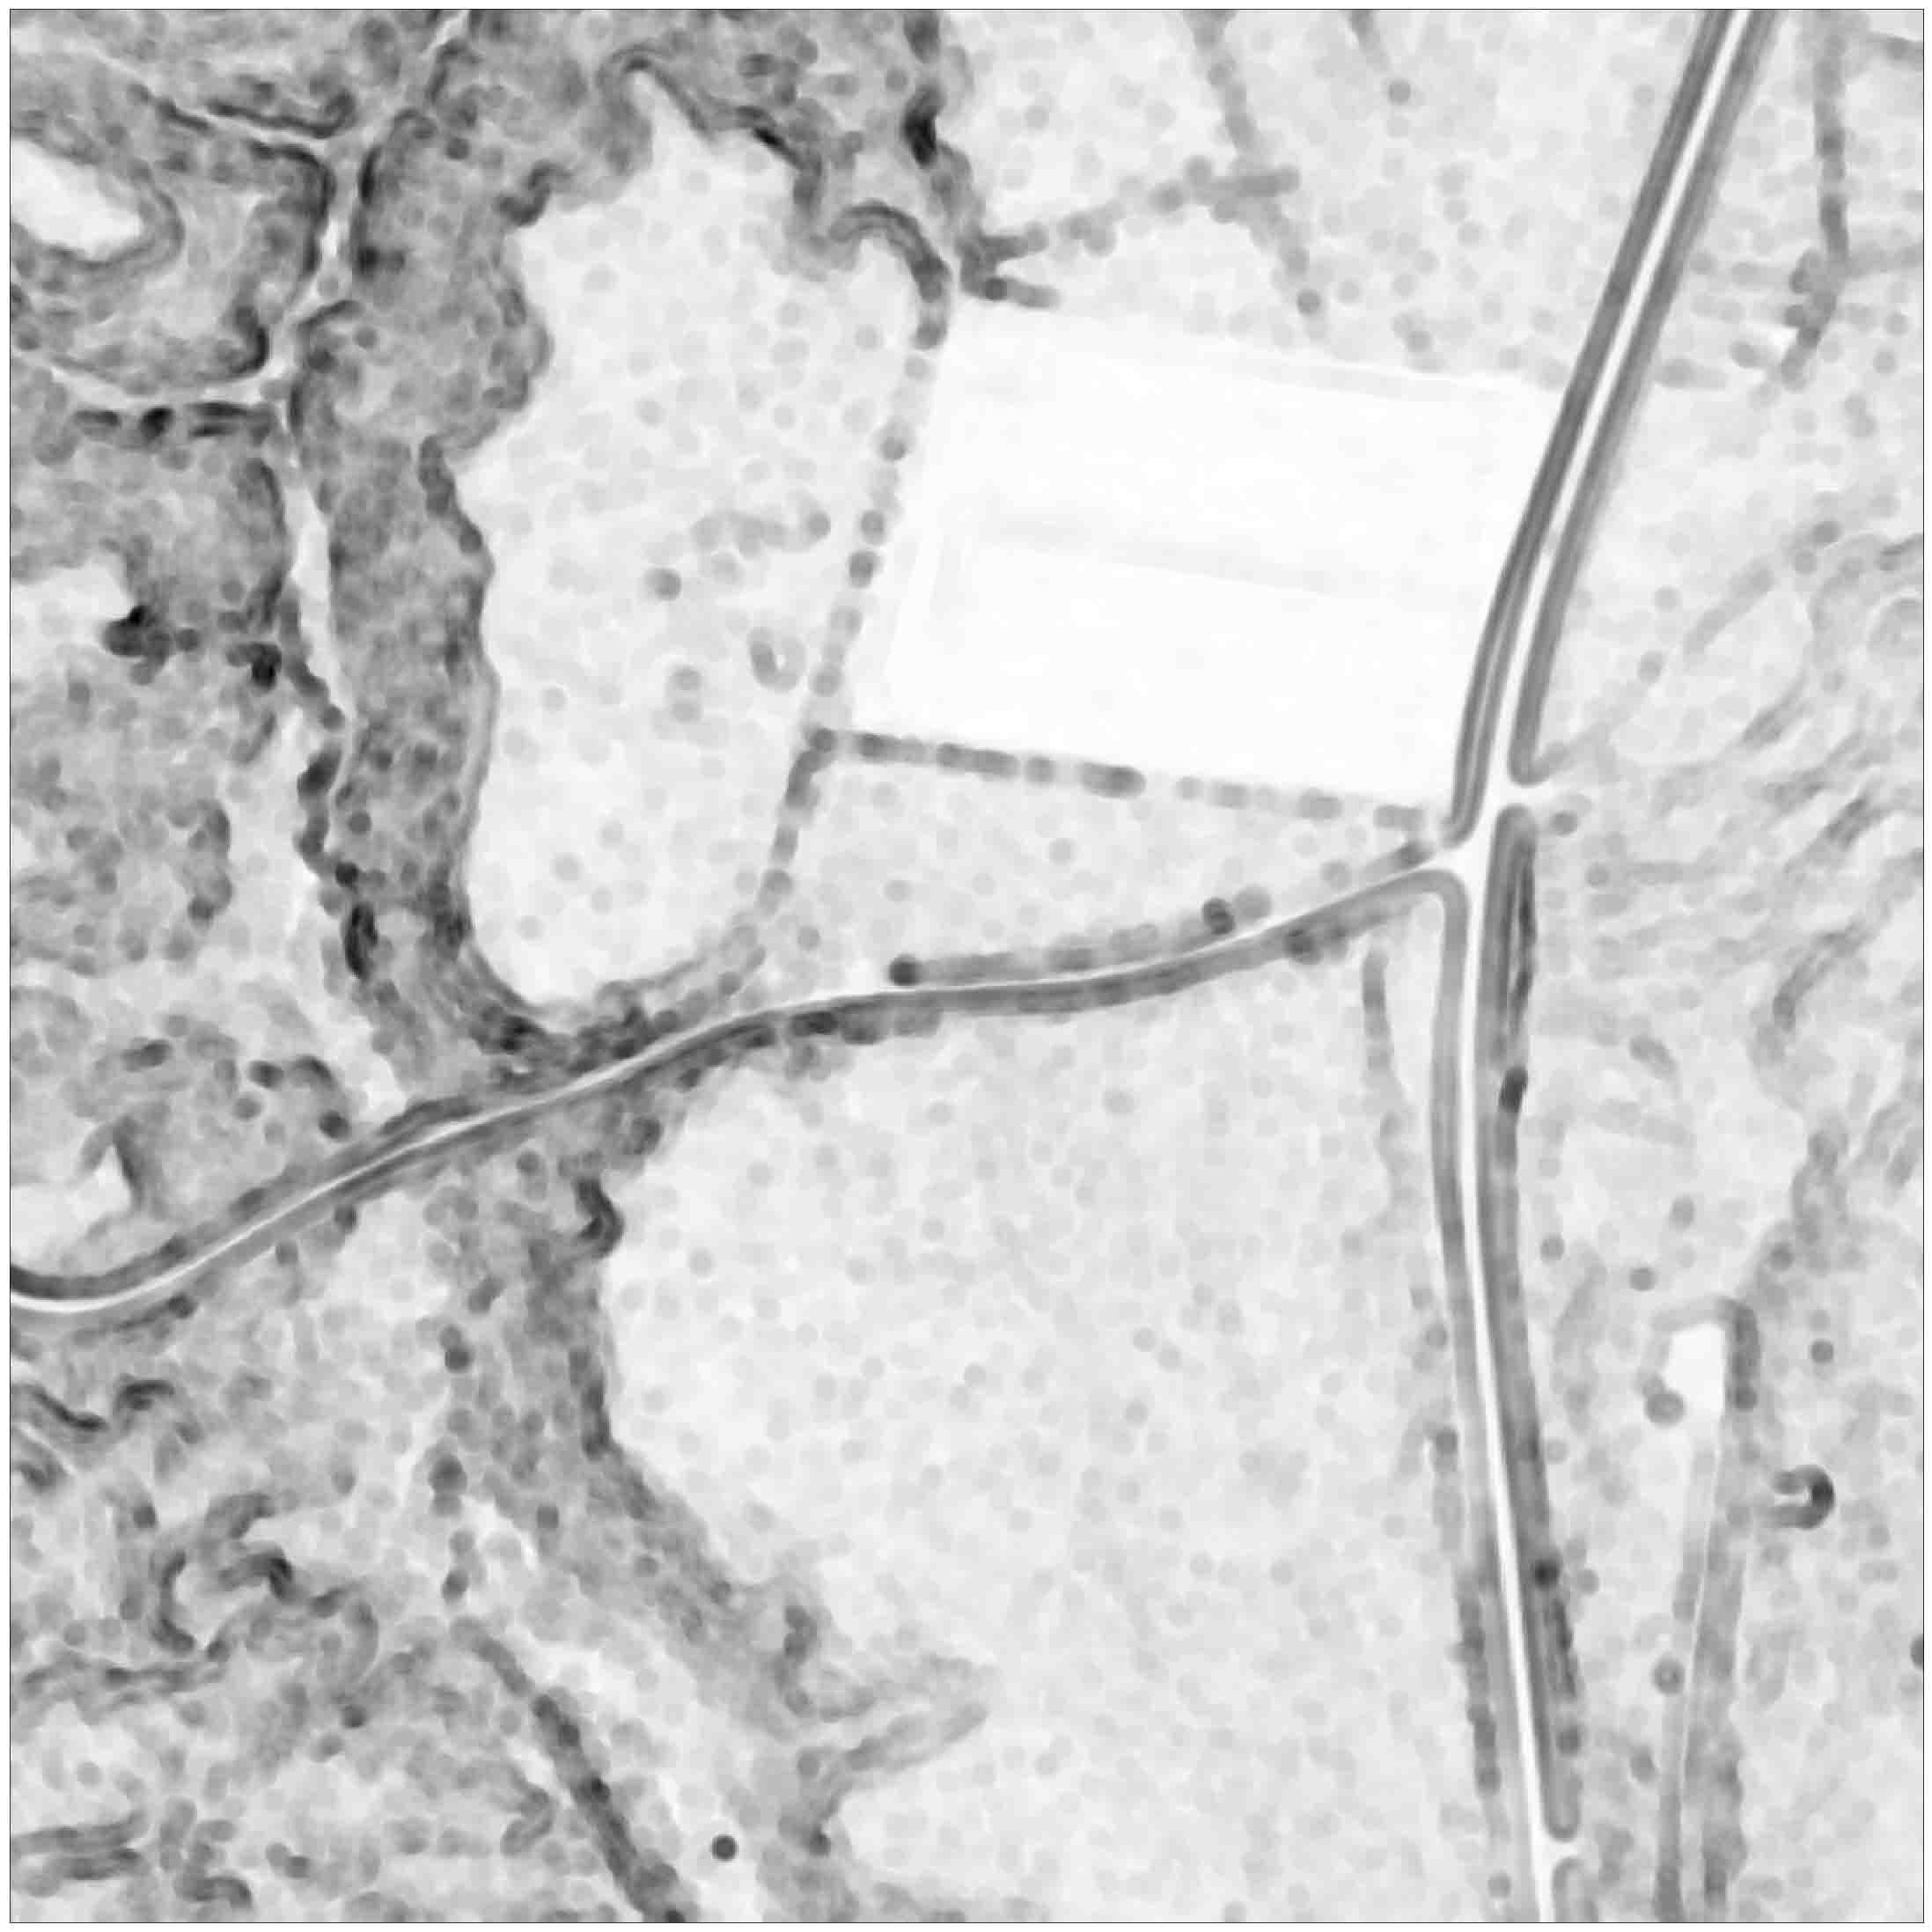
\includegraphics{./images/feature_b_lo.jpg}}}
    \subfigure[]{
        \resizebox*{3.5cm}{!}{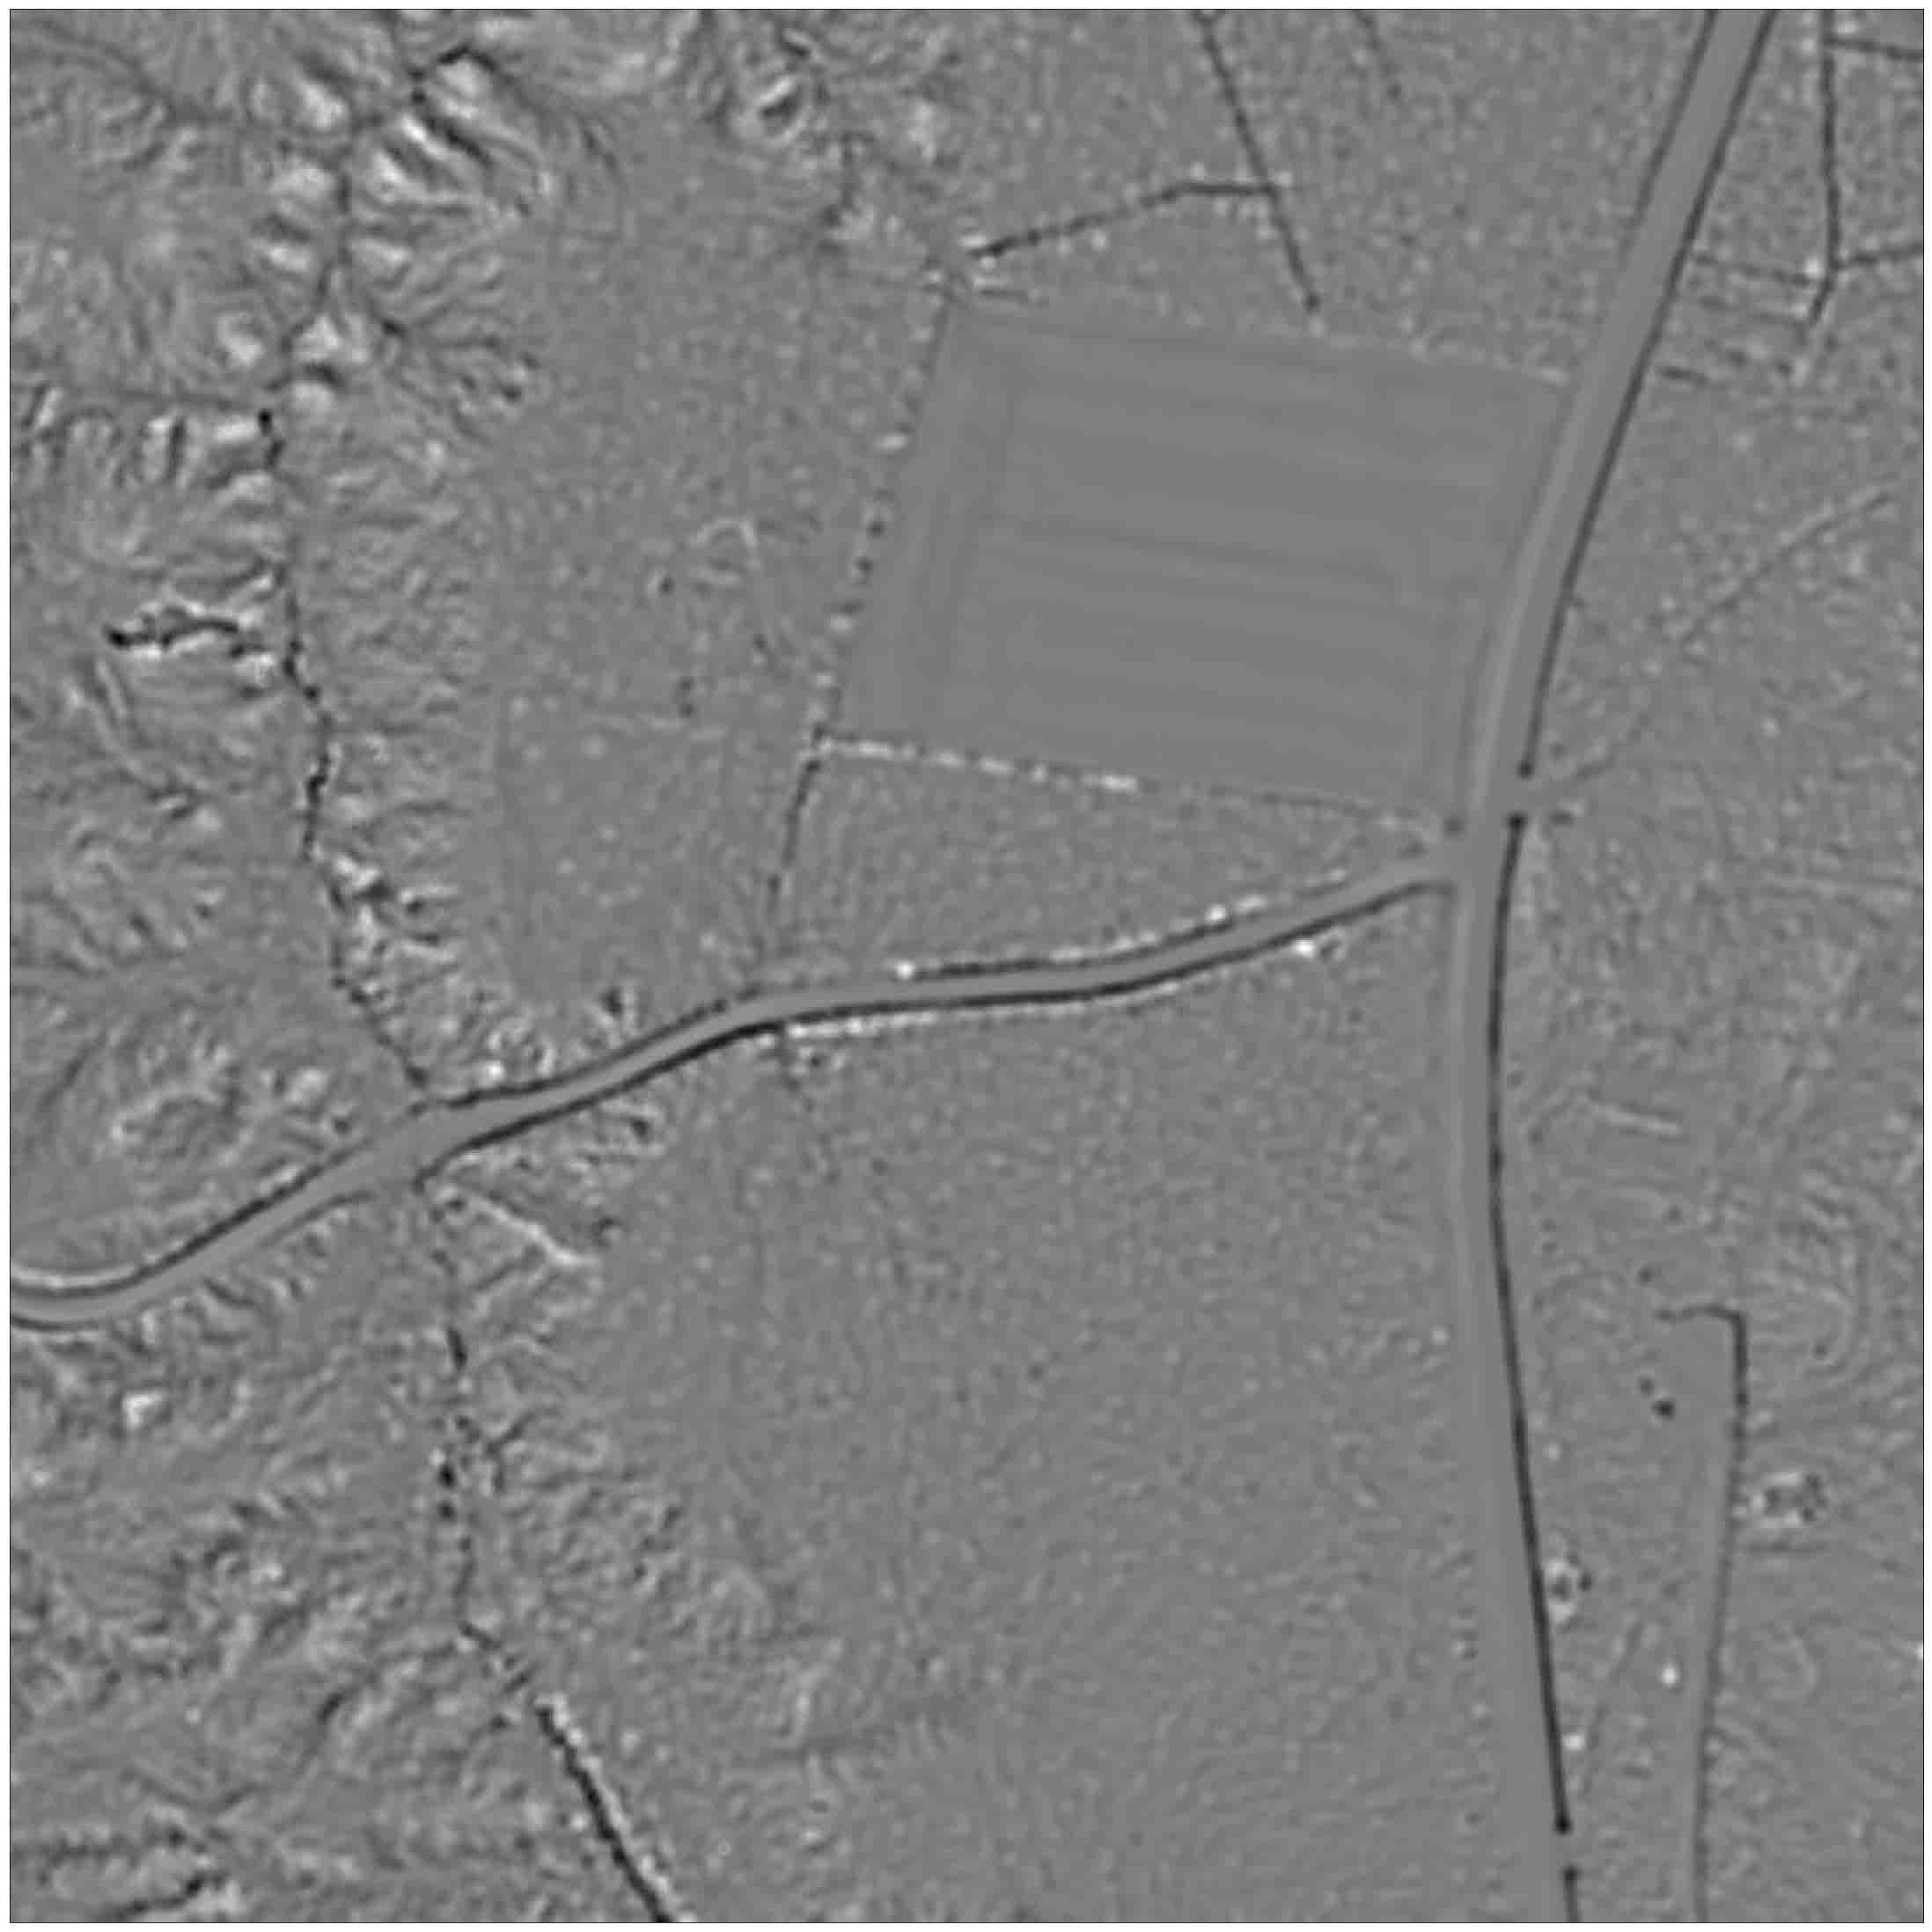
\includegraphics{./images/feature_c_lo.jpg}}}
    \subfigure[]{
        \resizebox*{3.5cm}{!}{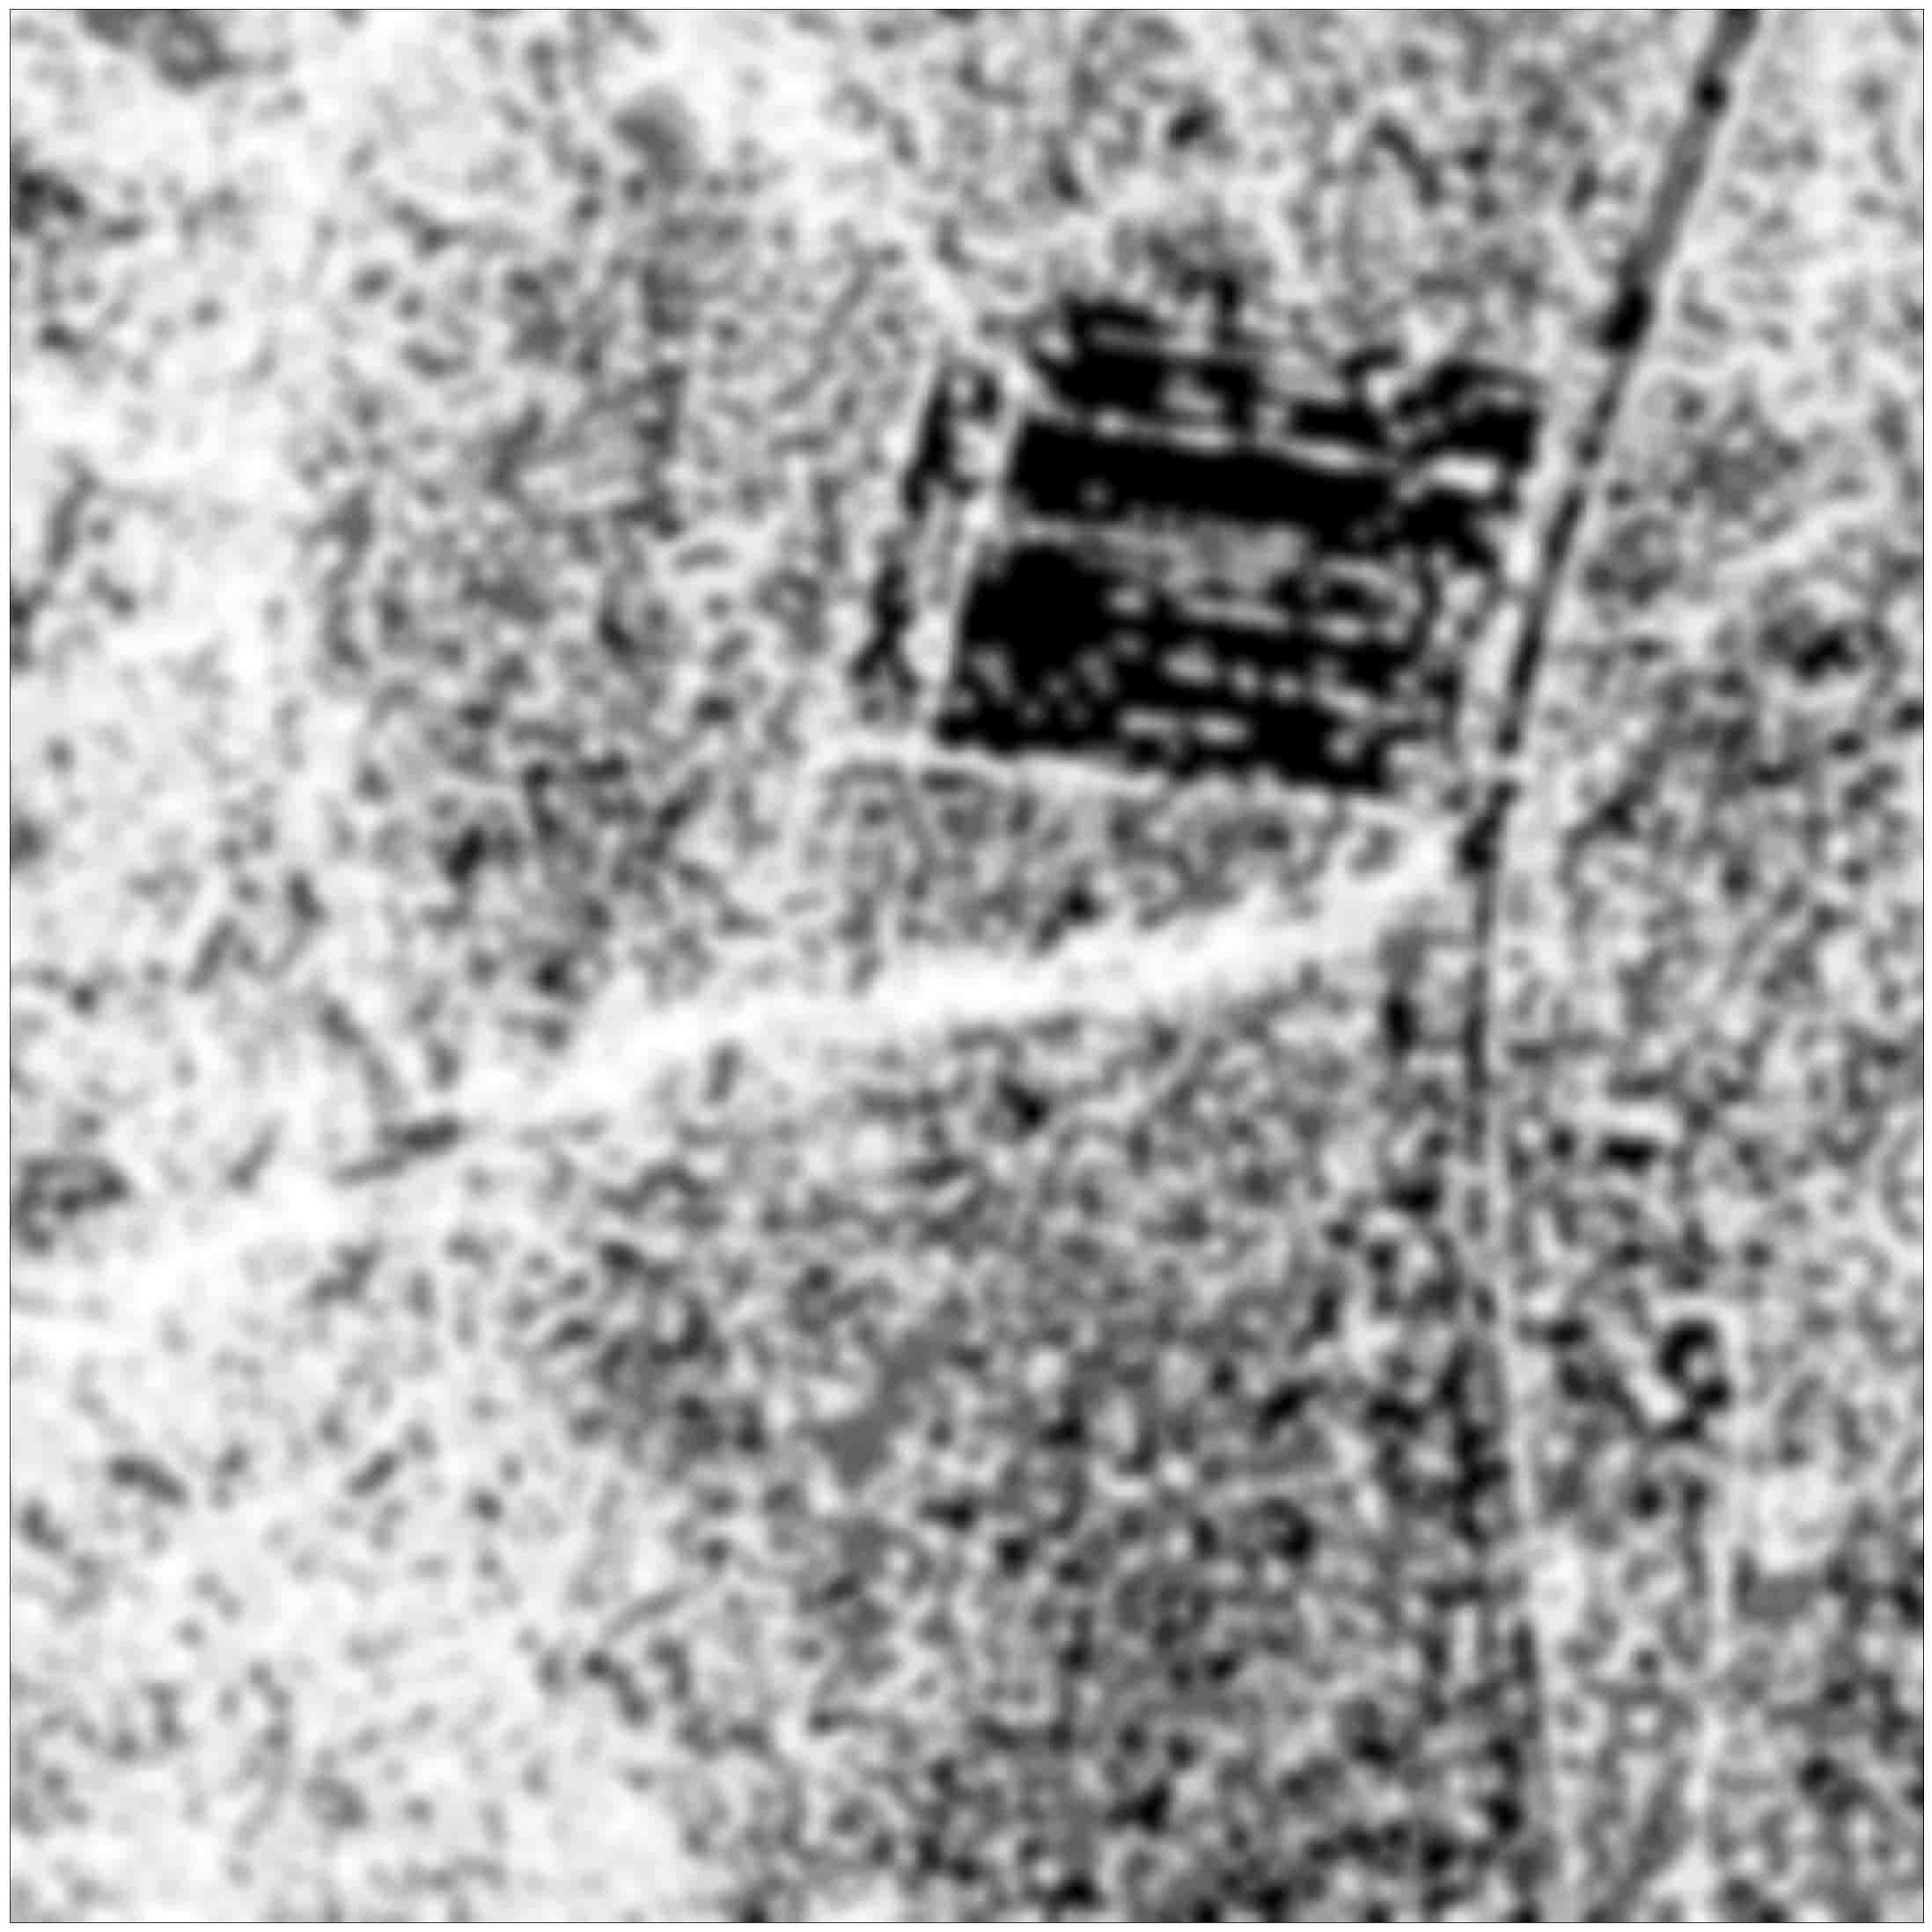
\includegraphics{./images/feature_d_lo.jpg}}}
    \subfigure[]{
        \resizebox*{3.5cm}{!}{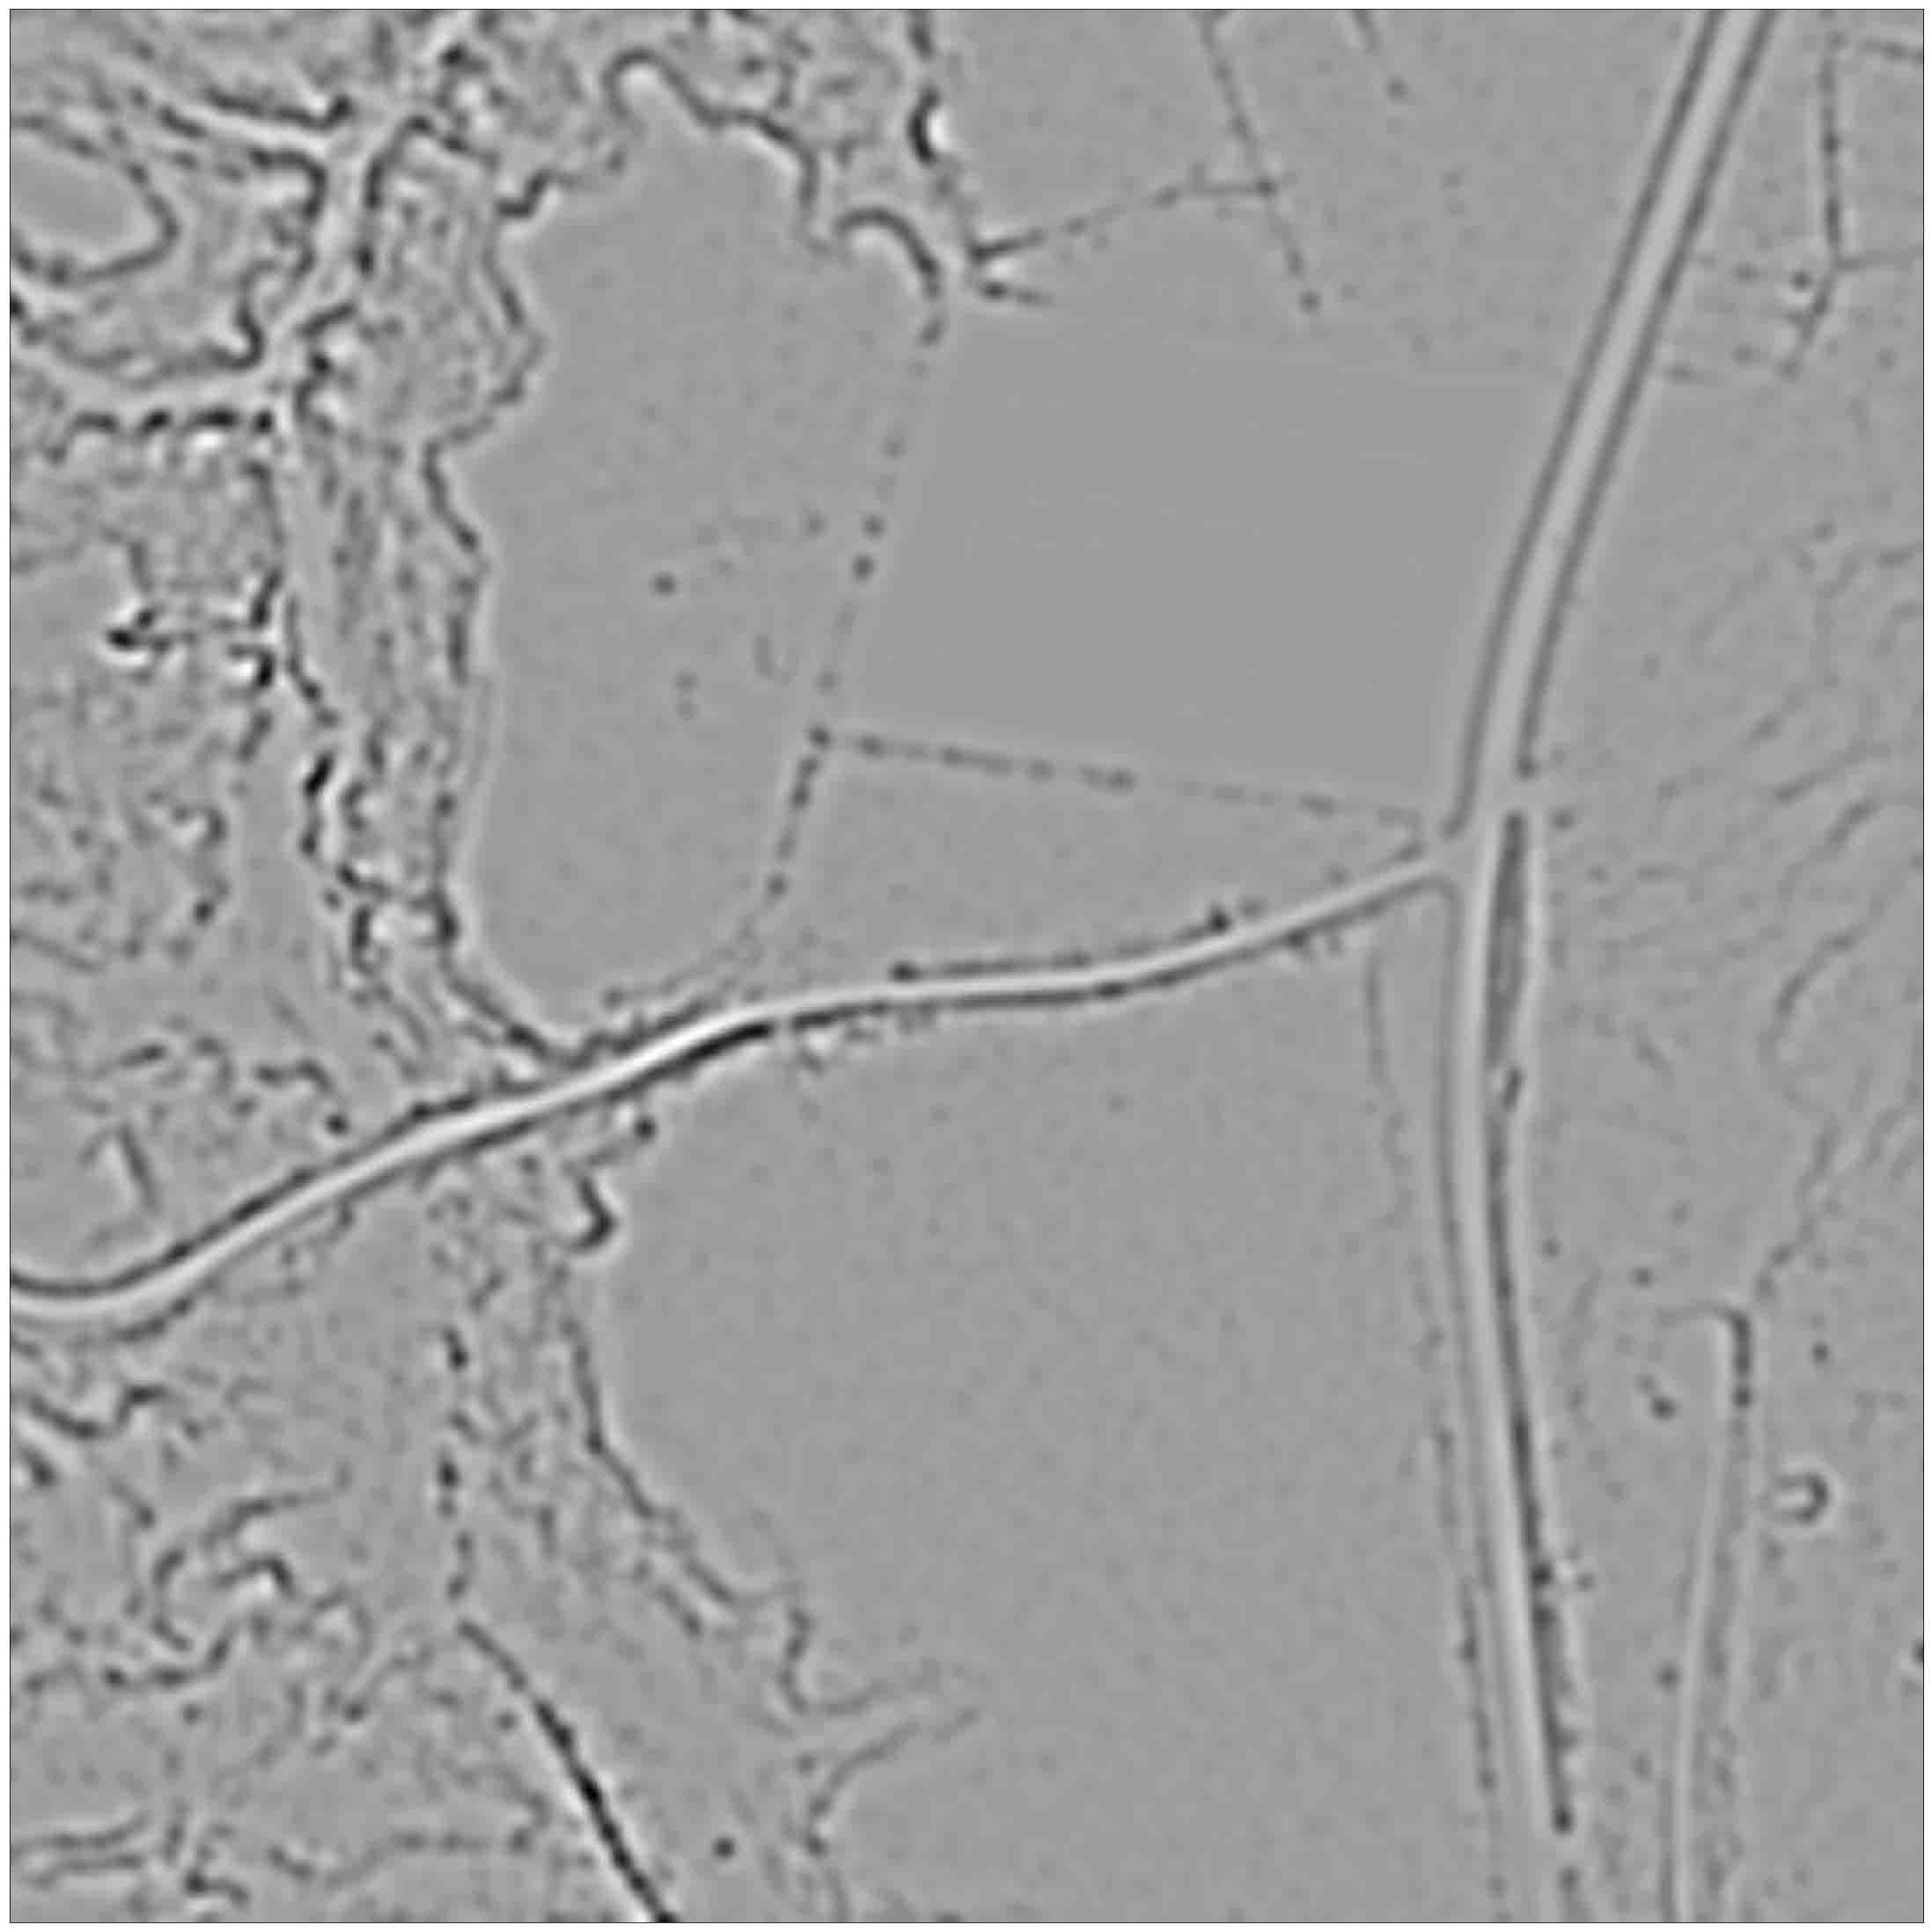
\includegraphics{./images/feature_e_lo.jpg}}}
    \subfigure[]{
        \resizebox*{3.5cm}{!}{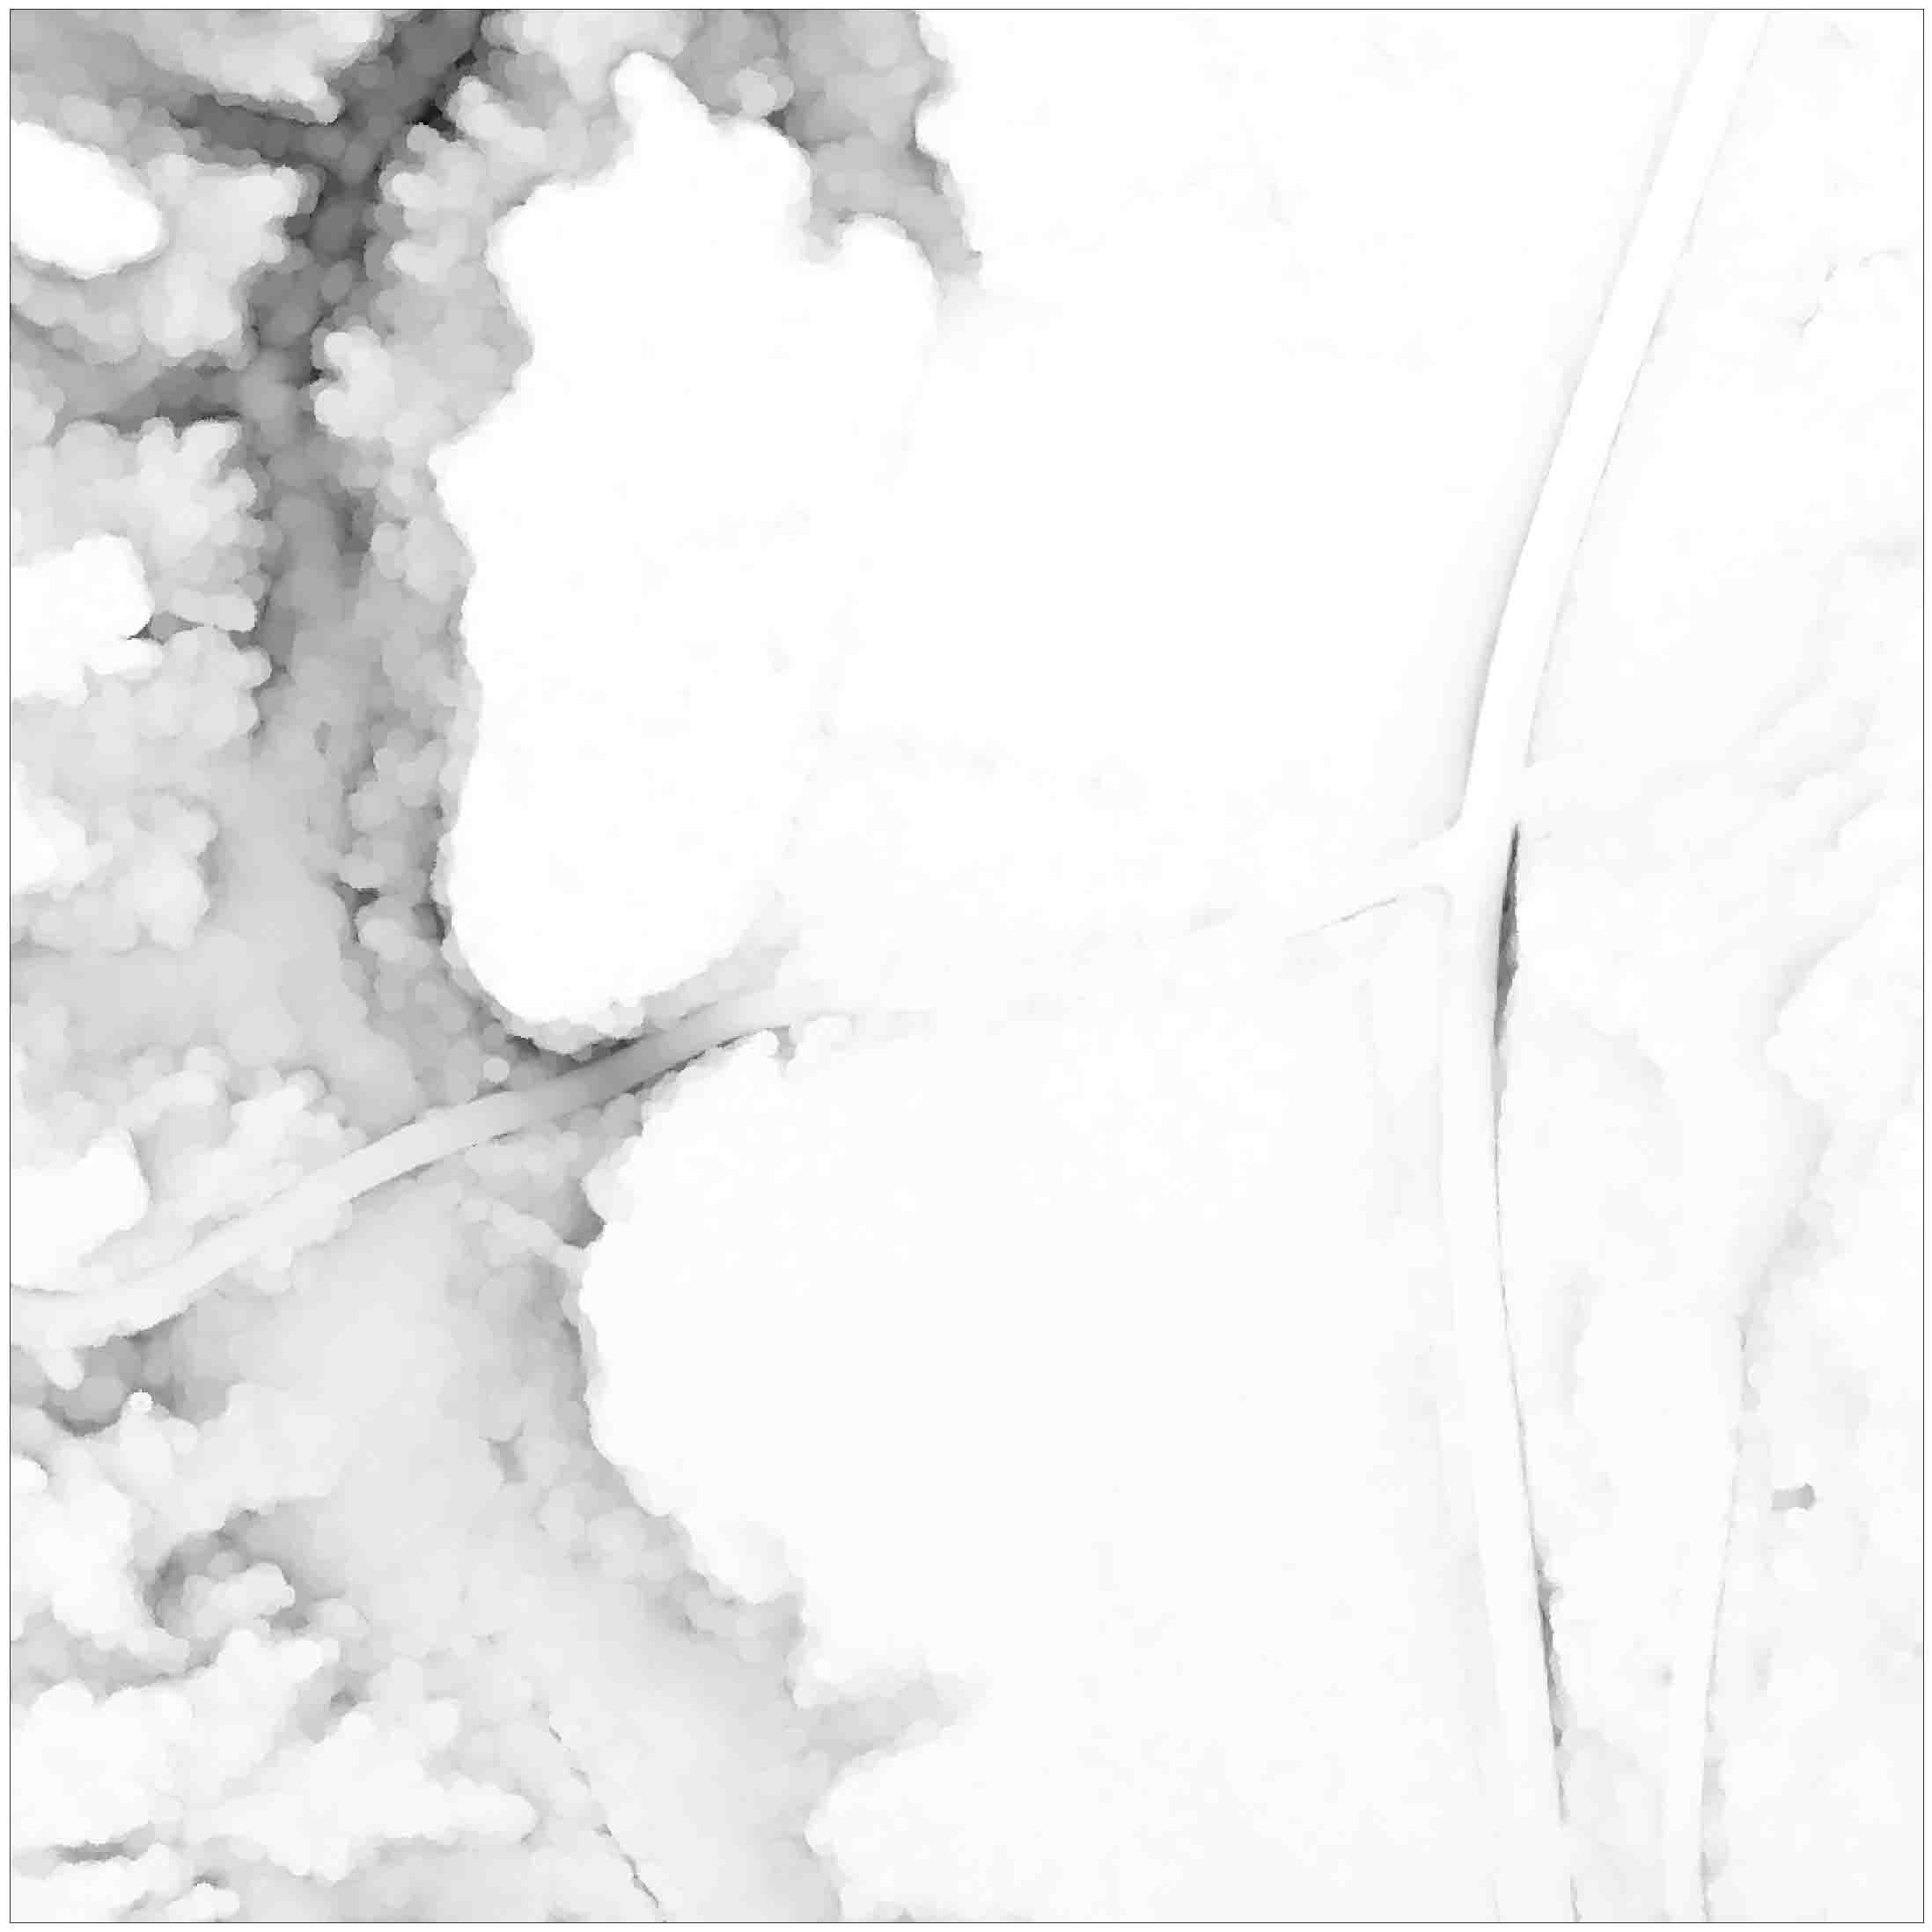
\includegraphics{./images/feature_f_lo.jpg}}}
    \subfigure[]{
        \resizebox*{3.5cm}{!}{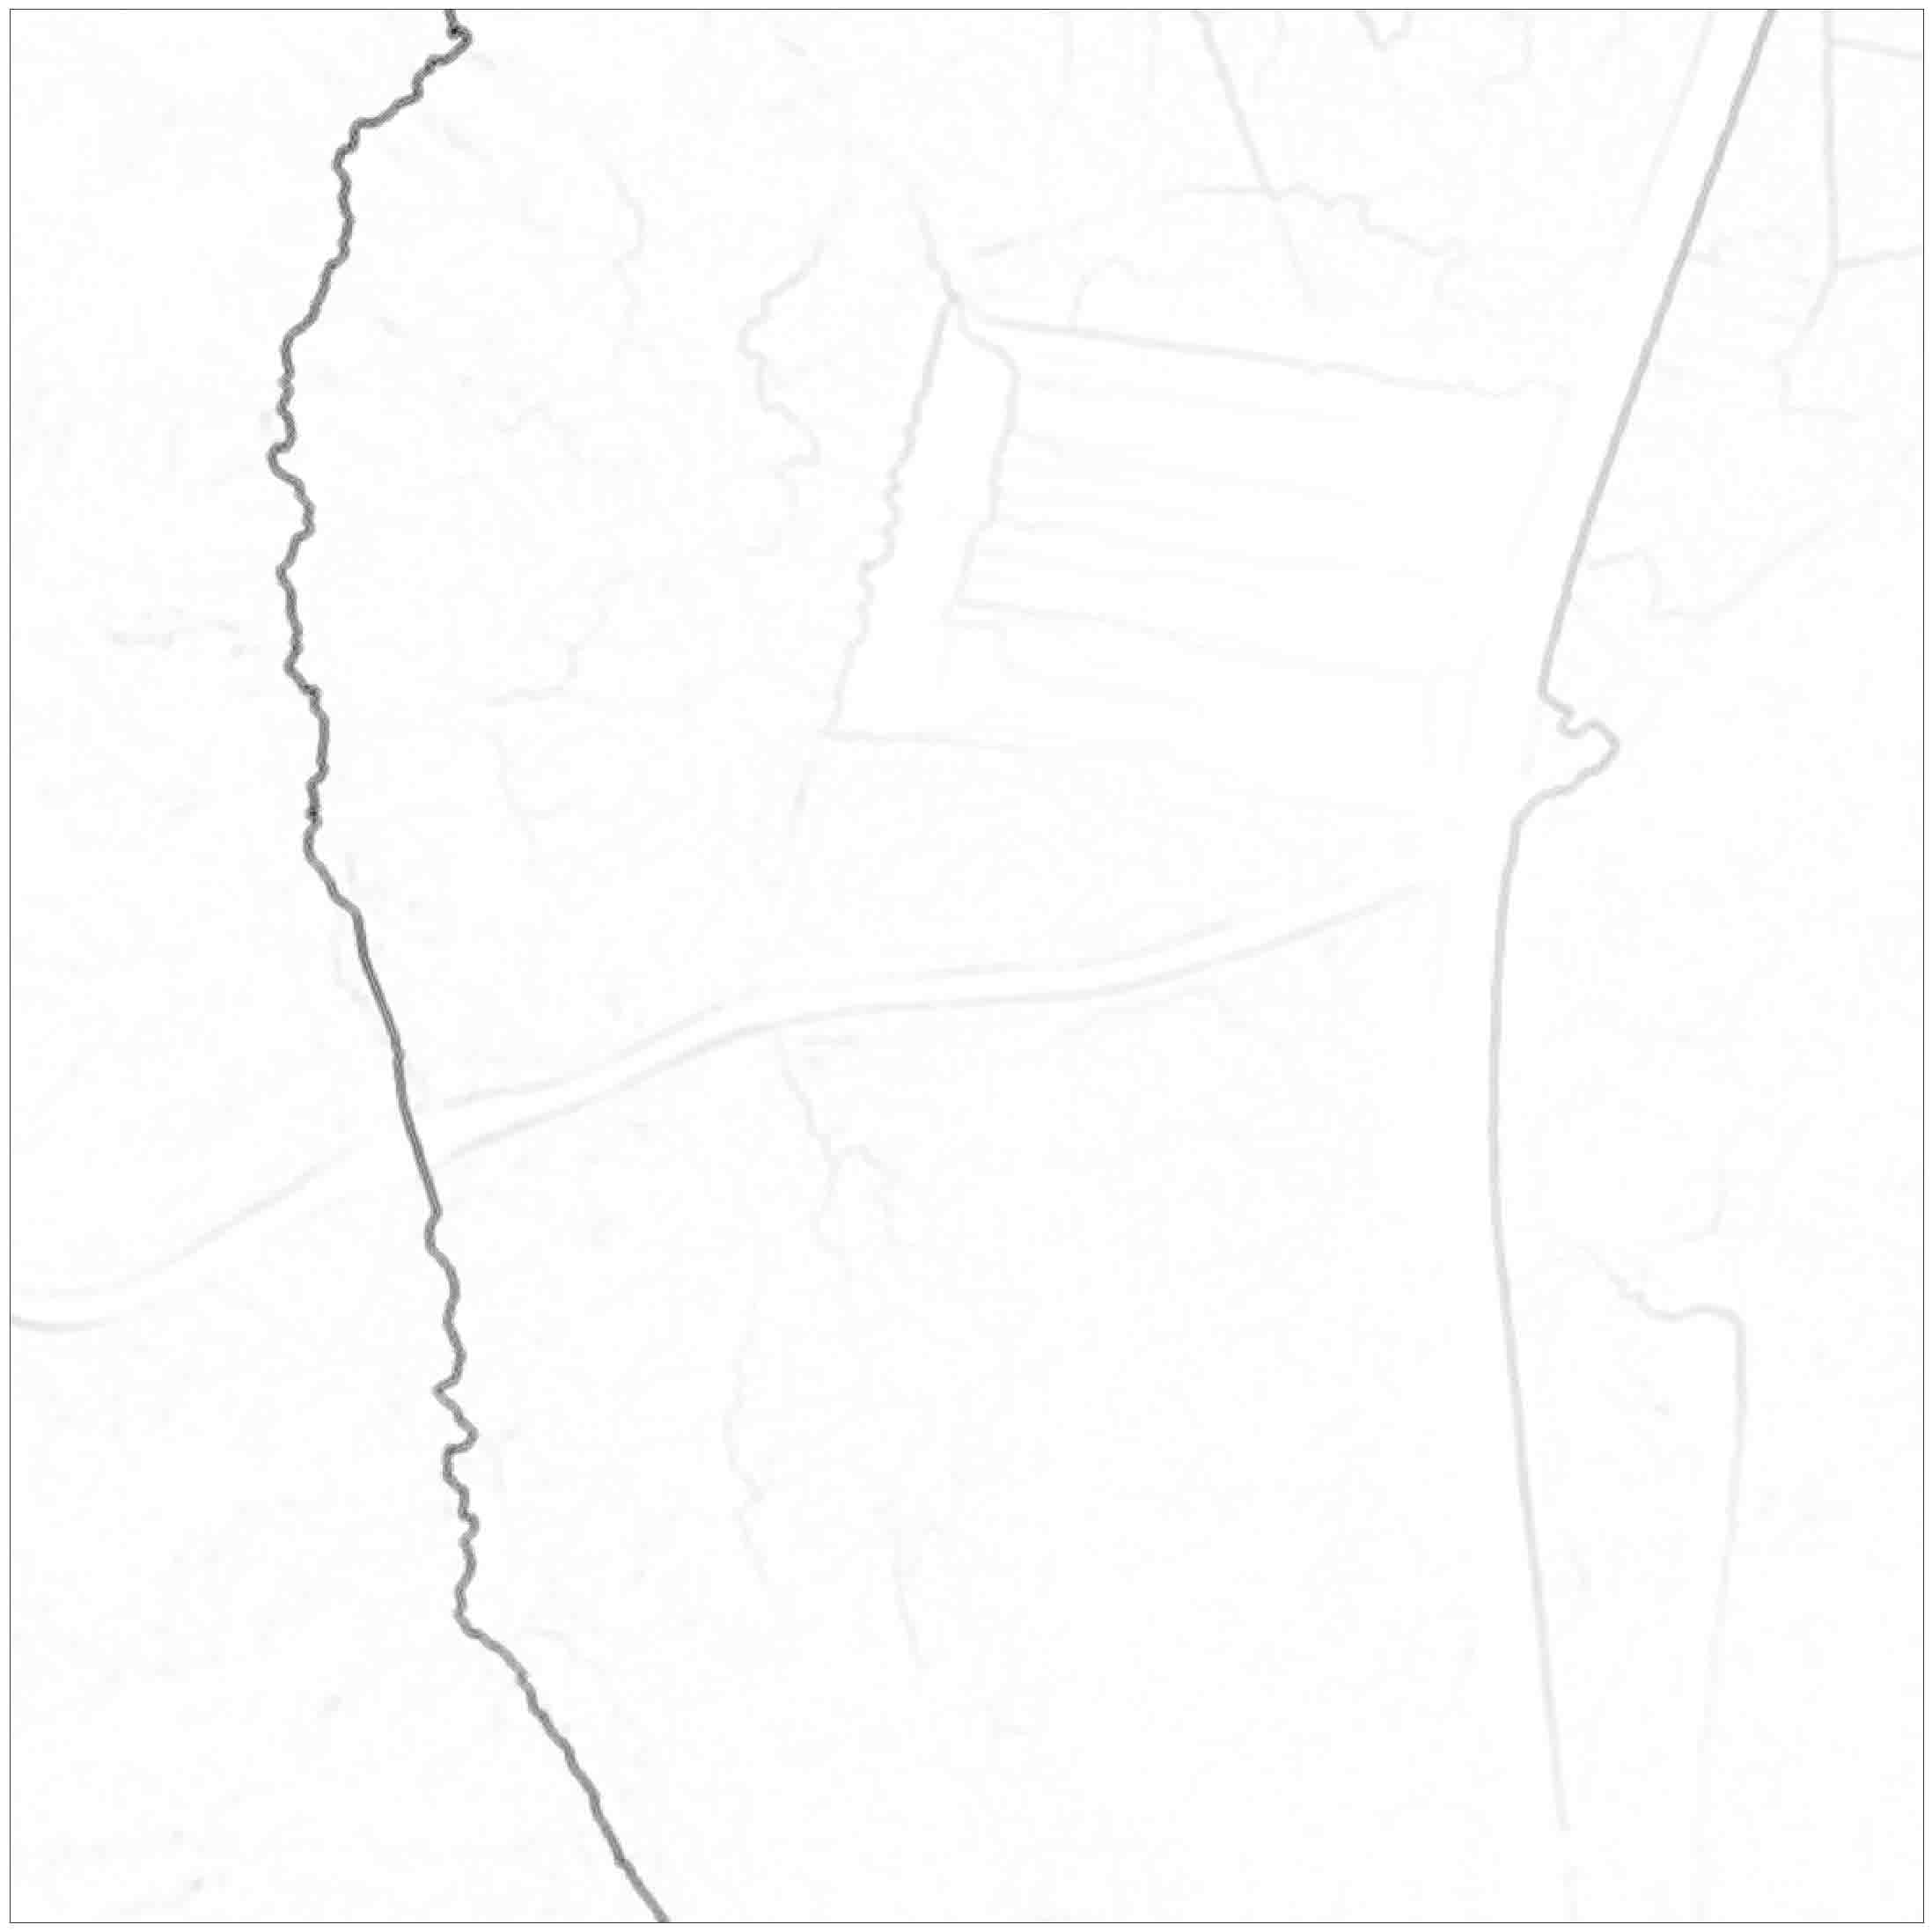
\includegraphics{./images/feature_g_lo.jpg}}}
    \subfigure[]{
        \resizebox*{3.5cm}{!}{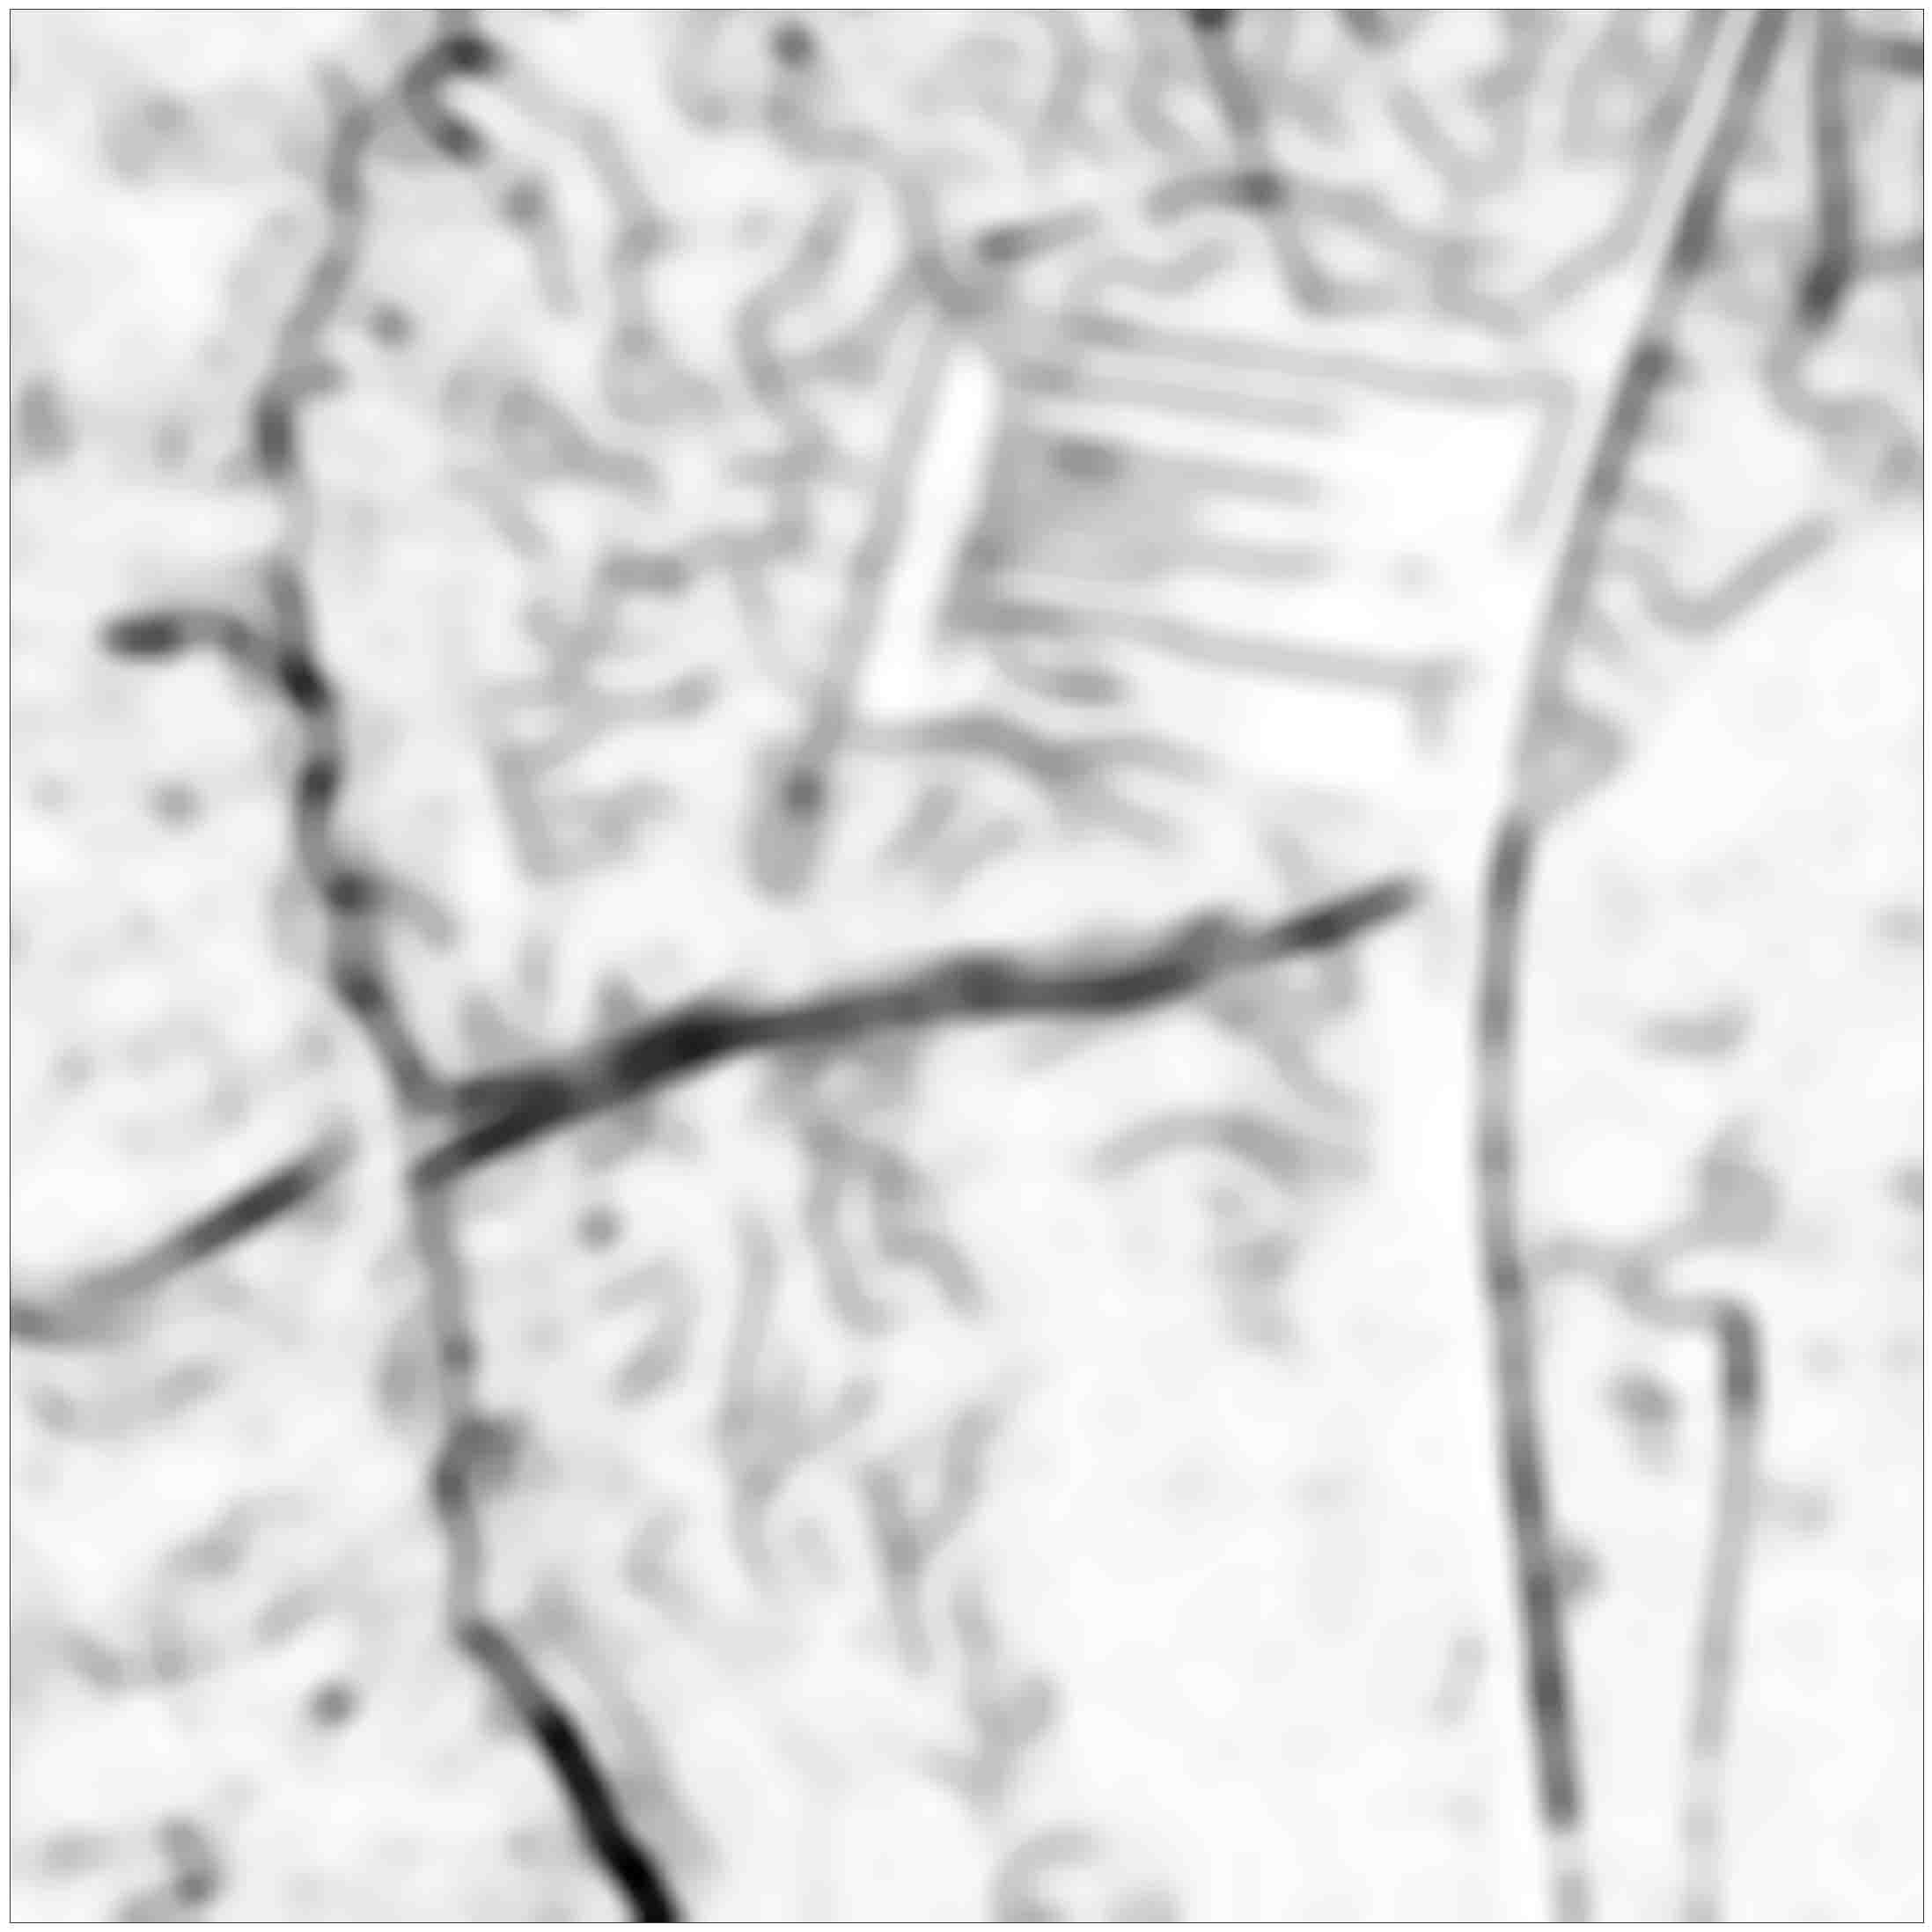
\includegraphics{./images/feature_h_lo.jpg}}}
    \subfigure[]{
        \resizebox*{3.5cm}{!}{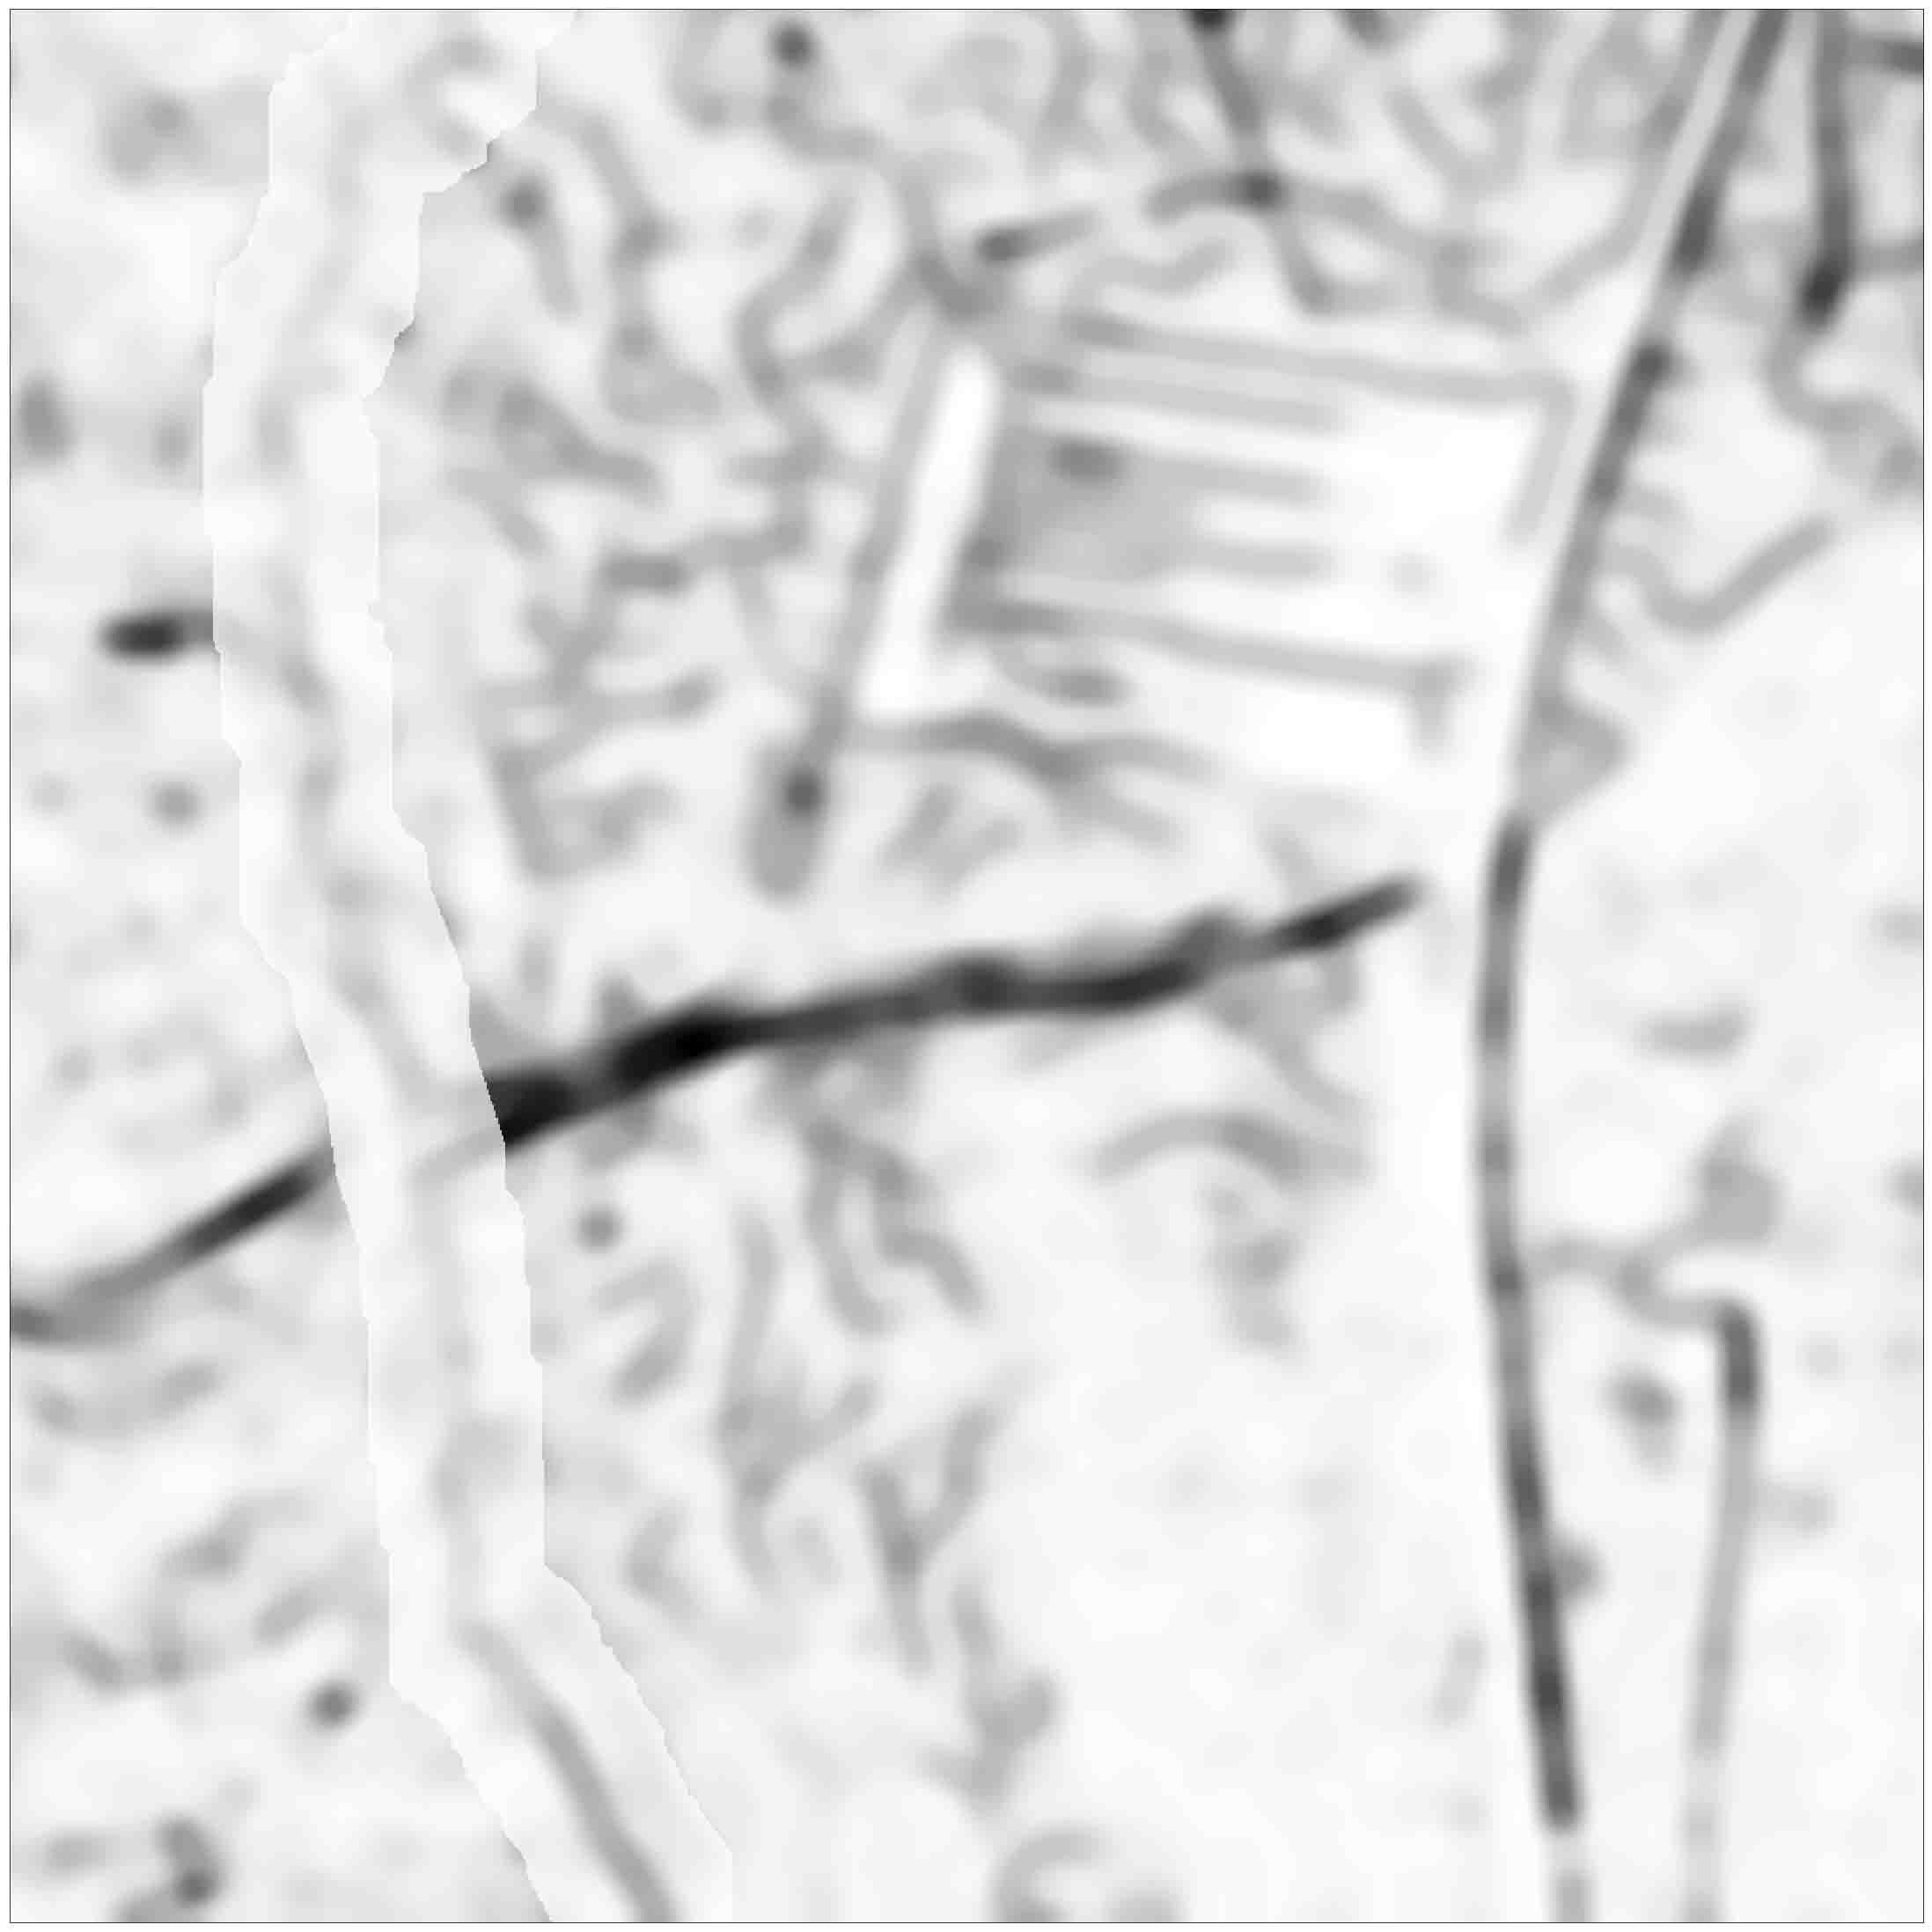
\includegraphics{./images/feature_i_lo.jpg}}}
    \DIFaddendFL \caption{\DIFdelbeginFL \DIFdelFL{Example of 8 of }\DIFdelendFL \DIFaddbeginFL \textbf{\DIFaddFL{Feature examples.}} \DIFaddFL{Shows }\DIFaddendFL the \DIFdelbeginFL \DIFdelFL{40 input variables, in addition to }\DIFdelendFL ditch labels \DIFdelbeginFL \DIFdelFL{used by }\DIFdelendFL \DIFaddbeginFL \DIFaddFL{as well as 8 of }\DIFaddendFL the \DIFdelbeginFL \DIFdelFL{models }\DIFdelendFL \DIFaddbeginFL \DIFaddFL{40 features }\DIFaddendFL for a small sample area. The radii represents pixels with a 0.5 m resolution. \newline \textbf{a:} Labelled ditches, \textbf{b:} Slope standard deviation, radius 6, \textbf{c:} HPMF mean, radius 4, \textbf{d:} HPMF ditch amplification, \textbf{e:} Sky View Factor Gabor, \textbf{f:} Sky View Factor max, radius 6, \textbf{g:} Impoundment mean, radius 3, \textbf{h:} Impoundment ditch amplification, \textbf{i:} Impoundment ditch amplification - streams removed}
    \label{fig:features}
\end{figure}

\subsubsection{Training and validation datasets}
\label{trainingvalidationdatasets}
To develop and evaluate our ditch detector, the raster and ditch label data of Krycklan were manually divided into 21 subsections\DIFdelbegin \DIFdel{. Each subsection represents }\DIFdelend \DIFaddbegin \DIFadd{, each representing }\DIFaddend an area of roughly 196 hectare \DIFdelbegin \DIFdel{. From this division, }\DIFdelend \DIFaddbegin \DIFadd{(}\hyperref[fig:swedenkrycklan]{Figure} \DIFadd{\ref{fig:swedenkrycklan}). This was necessary because our method relies on the area surrounding a pixel for feature extraction, meaning it is not possible to select random pixels for training and testing. }\DIFaddend 11 of the subsections were put aside as hold-out data, only for use in the experiment to evaluate the performance of the \DIFdelbegin \DIFdel{predictions}\DIFdelend \DIFaddbegin \DIFadd{ditch detector}\DIFaddend . The remaining 10 subsections were used solely before the experiment to develop the ditch detector\DIFaddbegin \DIFadd{, and }\DIFaddend to test different ways of preparing the data. This allowed the ditch detector to be evaluated on independent data\DIFdelbegin \DIFdel{and  strengthened }\DIFdelend \DIFaddbegin \DIFadd{, strengthening }\DIFaddend the validity of the experiment. \hyperref[fig:swedenkrycklan]{Figure} \ref{fig:swedenkrycklan} shows which subsections were used for development and evaluation respectively. \DIFdelbegin %DIFDELCMD < 

%DIFDELCMD < %%%
\DIFdel{Using the }\DIFdelend \DIFaddbegin \DIFadd{The }\DIFaddend 11 \DIFdelbegin \DIFdel{subsections in the hold-out data for the final experiment, a process called }\textit{\DIFdel{k-fold cross validation}} %DIFAUXCMD
\DIFdel{was employed (}\DIFdelend \DIFaddbegin \DIFadd{hold-out subsections were used as folds in an }\DIFaddend 11-fold cross validation in \DIFdelbegin \DIFdel{our case). K-fold cross validation is a method where you divide your dataset into folds of similar size and train a model on all but one of your folds (subsections). You then use that subsection to evaluate the results \mbox{%DIFAUXCMD
\citep{crossvalidation}}\hspace{0pt}%DIFAUXCMD
.
A new model is trained using the training folds for each iteration (}%DIFDELCMD < \hyperref[fig:crossvalidation]{Figure} %%%
\DIFdel{\ref{fig:crossvalidation}). Using this technique, shifting which subsection to leave out from the training, allowed us to train 11 different Random Forests classifying models with a large amount of data from the remaining 10 subsections in the hold-out data, producing 11 independent sub-experiments to evaluate the method on .
}\DIFdelend \DIFaddbegin \DIFadd{the final experiment.
}\DIFaddend 

\DIFdelbegin %DIFDELCMD < \begin{figure}[!htb]
%DIFDELCMD <     \centering
%DIFDELCMD <     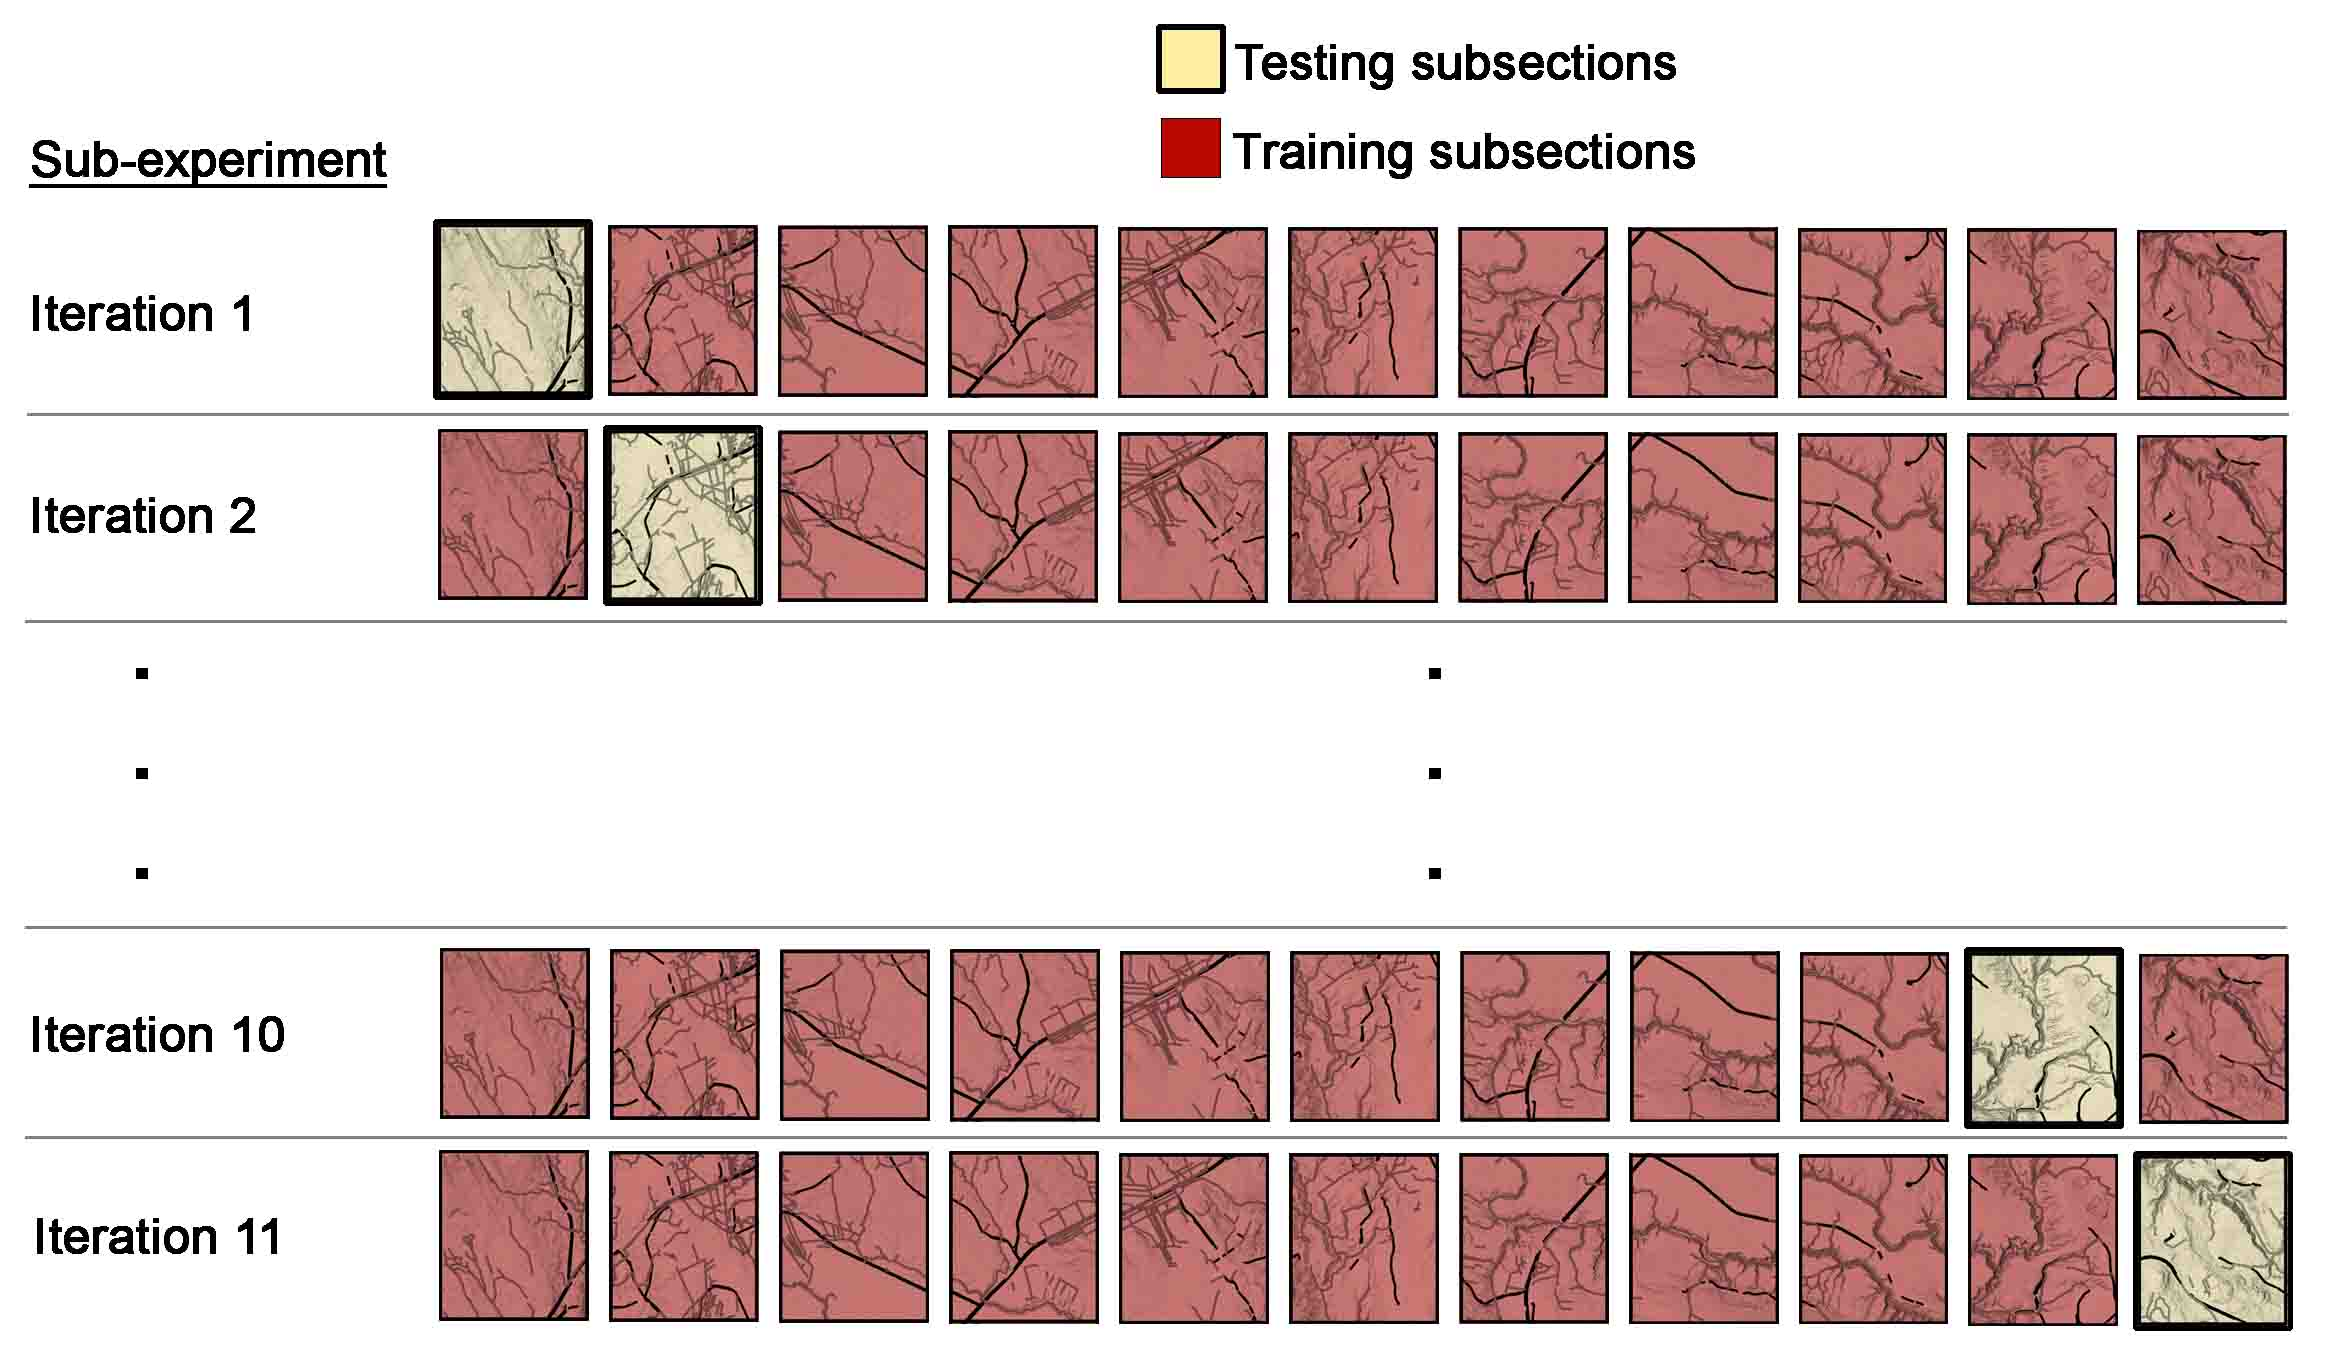
\includegraphics[width=1\linewidth]{images/cross_validation_lo.jpg}
%DIFDELCMD <     %%%
%DIFDELCMD < \caption{%
{%DIFAUXCMD
\DIFdelFL{11-fold cross validation. Each subsection in the hold-out data was used once for testing, with the remaining subsections being used to build a new model for each iteration.}}
    %DIFAUXCMD
%DIFDELCMD < \label{fig:crossvalidation}
%DIFDELCMD < \end{figure}
%DIFDELCMD < 

%DIFDELCMD < %%%
\DIFdelend \subsection{Developing the Random Forests model}

\DIFdelbegin \DIFdel{Random Forests is an ensemble machine learning method which builds multiple diverse decision trees to increase the robustness of its predictions \mbox{%DIFAUXCMD
\citep{breiman,flach}}\hspace{0pt}%DIFAUXCMD
. The individual trees are trained by minimising the entropy of the data from each node’s output \mbox{%DIFAUXCMD
\citep{kotsiantis}}\hspace{0pt}%DIFAUXCMD
. }\DIFdelend \DIFaddbegin \DIFadd{The Random Forests \mbox{%DIFAUXCMD
\citep{breiman} }\hspace{0pt}%DIFAUXCMD
algorithm from the Python library }\textit{\DIFadd{scikit-learn}} \DIFadd{\mbox{%DIFAUXCMD
\citep{scikit-learn} }\hspace{0pt}%DIFAUXCMD
was used in the experiment, and the classifiers were trained on the 40 features seen in }\hyperref[featuretable]{Table} \DIFadd{\ref{featuretable}. }\DIFaddend A byproduct of the training is the Gini importance, which denotes the most important \DIFdelbegin \DIFdel{input variables }\DIFdelend \DIFaddbegin \DIFadd{features }\DIFaddend \citep{gini}. For our study, a hyperparameter tuning showed that using 300 trees and \textit{gini} as the splitting criterion, with a minimum of 10 samples per node split, and no artificial class weight or max depth of trees yielded the best predictions. The \DIFdelbegin \DIFdel{Random Forests algorithm from the Python library }\textit{\DIFdel{scikit-learn}} %DIFAUXCMD
\DIFdel{\mbox{%DIFAUXCMD
\citep{scikit-learn} }\hspace{0pt}%DIFAUXCMD
was used in the experiment, and the classifiers were trained on all the input variables seen in }%DIFDELCMD < \hyperref[featuretable]{Table} %%%
\DIFdel{\ref{featuretable}}\DIFdelend \DIFaddbegin \DIFadd{testing phase showed that, due to the class imbalance (only 2\% of pixels being ditch pixels), the model was not being punished for mislabelling ditches as non-ditches. To combat this, we evened out the amount of ditch and non-ditch instances in the training data by first extracting all pixels labelled as ditches as well as pixels within close proximity of ditches. Second, pixels were sampled randomly from the entire subsection to still capture most of the geographical features of each area (}\hyperref[fig:balancedmasks]{Figure} \DIFadd{\ref{fig:balancedmasks})}\DIFaddend .

\begin{table} [!htb]
\DIFdelbeginFL %DIFDELCMD < \tbl{The 40 input variables used when training the models.}
%DIFDELCMD <     %%%
\DIFdelendFL \DIFaddbeginFL \centering
    \DIFaddendFL {\begin{tabular}{ll}
      \DIFdelbeginFL %DIFDELCMD < \toprule
%DIFDELCMD <       %%%
\DIFdelFL{Variable/Algorithm}\DIFdelendFL \DIFaddbeginFL \textbf{\DIFaddFL{Terrain Index/Algorithm}}\DIFaddendFL \textsuperscript{a} & \DIFdelbeginFL \DIFdelFL{Circular radii}\DIFdelendFL \DIFaddbeginFL \textbf{\DIFaddFL{Circular radii}}\DIFaddendFL \textsuperscript{b} \\ 
      \DIFdelbeginFL %DIFDELCMD < \midrule
%DIFDELCMD <       

%DIFDELCMD <       %%%
\DIFdelendFL \DIFaddbeginFL \hline
      \DIFaddendFL Sky View Factor median &2, 6 \\
      Sky View Factor standard deviation & 6 \\
      Sky View Factor min & 6 \\
      Sky View Factor max & 2, 4, 6 \\
      Sky View Factor non ditch amplification & - \\ 
      Sky View Factor Gabor & - \\
      Sky View Factor Gabor - streams removed & -\\

      Impoundment mean & 2, 3, 4, 6 \\
      Impoundment median & 2, 4, 6 \\
      Impoundment standard deviation & 4, 6 \\
      Impoundment max & 6 \\
      Impoundment ditch amplification & - \\
      Impoundment ditch amplification - streams removed & - \\

      HPMF mean & 3, 4, 6 \\
      HPMF median & 4 \\
      HPMF standard deviation & 6 \\
      HPMF min & 2, 4 \\
      HPMF ditch amplification & - \\
      HPMF ditch amplification - streams removed & - \\
      HPMF Gabor - streams removed & -\\

      Slope mean & 6 \\
      Slope median & 6 \\
      Slope standard deviation & 4, 6 \\
      Slope min & 2, 4, 6 \\
      Slope non-ditch amplification & - \\
      \DIFdelbeginFL %DIFDELCMD < \bottomrule
%DIFDELCMD <     %%%
\DIFdelendFL \DIFaddbeginFL \hline
    \DIFaddendFL \end{tabular}}
    \DIFdelbeginFL %DIFDELCMD < \tabnote{\textsuperscript{a} Displays algorithm used to produce the variable. \newline
%DIFDELCMD <         \textsuperscript{b} Represents the radius of the circular mask (if one was used) to determine \newline what neighbouring pixels to use in an algorithm. The radii represents pixels \newline \mbox{with a 0.5 m resolution.\itshape\ignorespaces}}
%DIFDELCMD <     %%%
\DIFdelendFL \DIFaddbeginFL \caption{\textbf{\DIFaddFL{Feature set.}} \DIFaddFL{The 40 features used to train the models.
    }\newline \DIFaddFL{\textsuperscript{a} The algorithm used to produce the feature. }\newline
        \DIFaddFL{\textsuperscript{b} Represents the radius of the circular mask (if one was used) to determine which neighbouring pixels to use in the aggregation. The radii represents pixels with a 0.5 m resolution.}}
    \DIFaddendFL \label{featuretable}
\end{table}

\DIFdelbegin \DIFdel{The testing phase showed that the classifiers produced poor results when the ratio of ditch versus non-ditch pixels in the training data was very high, as the models were not being punished for mislabelling ditches as non-ditches. To increase the recall, we evened out the amount of ditch and non-ditch instances in the training data. First, we extracted all pixels labelled as ditches as well as pixels within close proximity of ditches. Secondly, pixels were sampled randomly from the entire subsection to still contain most of the geographical features of each area (}%DIFDELCMD < \hyperref[fig:balancedmasks]{Figure} %%%
\DIFdel{\ref{fig:balancedmasks}).
}%DIFDELCMD < 

%DIFDELCMD < %%%
\DIFdelend \begin{figure} [!htb]
    \centering
    \DIFdelbeginFL %DIFDELCMD < \subfigure[]{
%DIFDELCMD <         \resizebox*{6.85cm}{!}{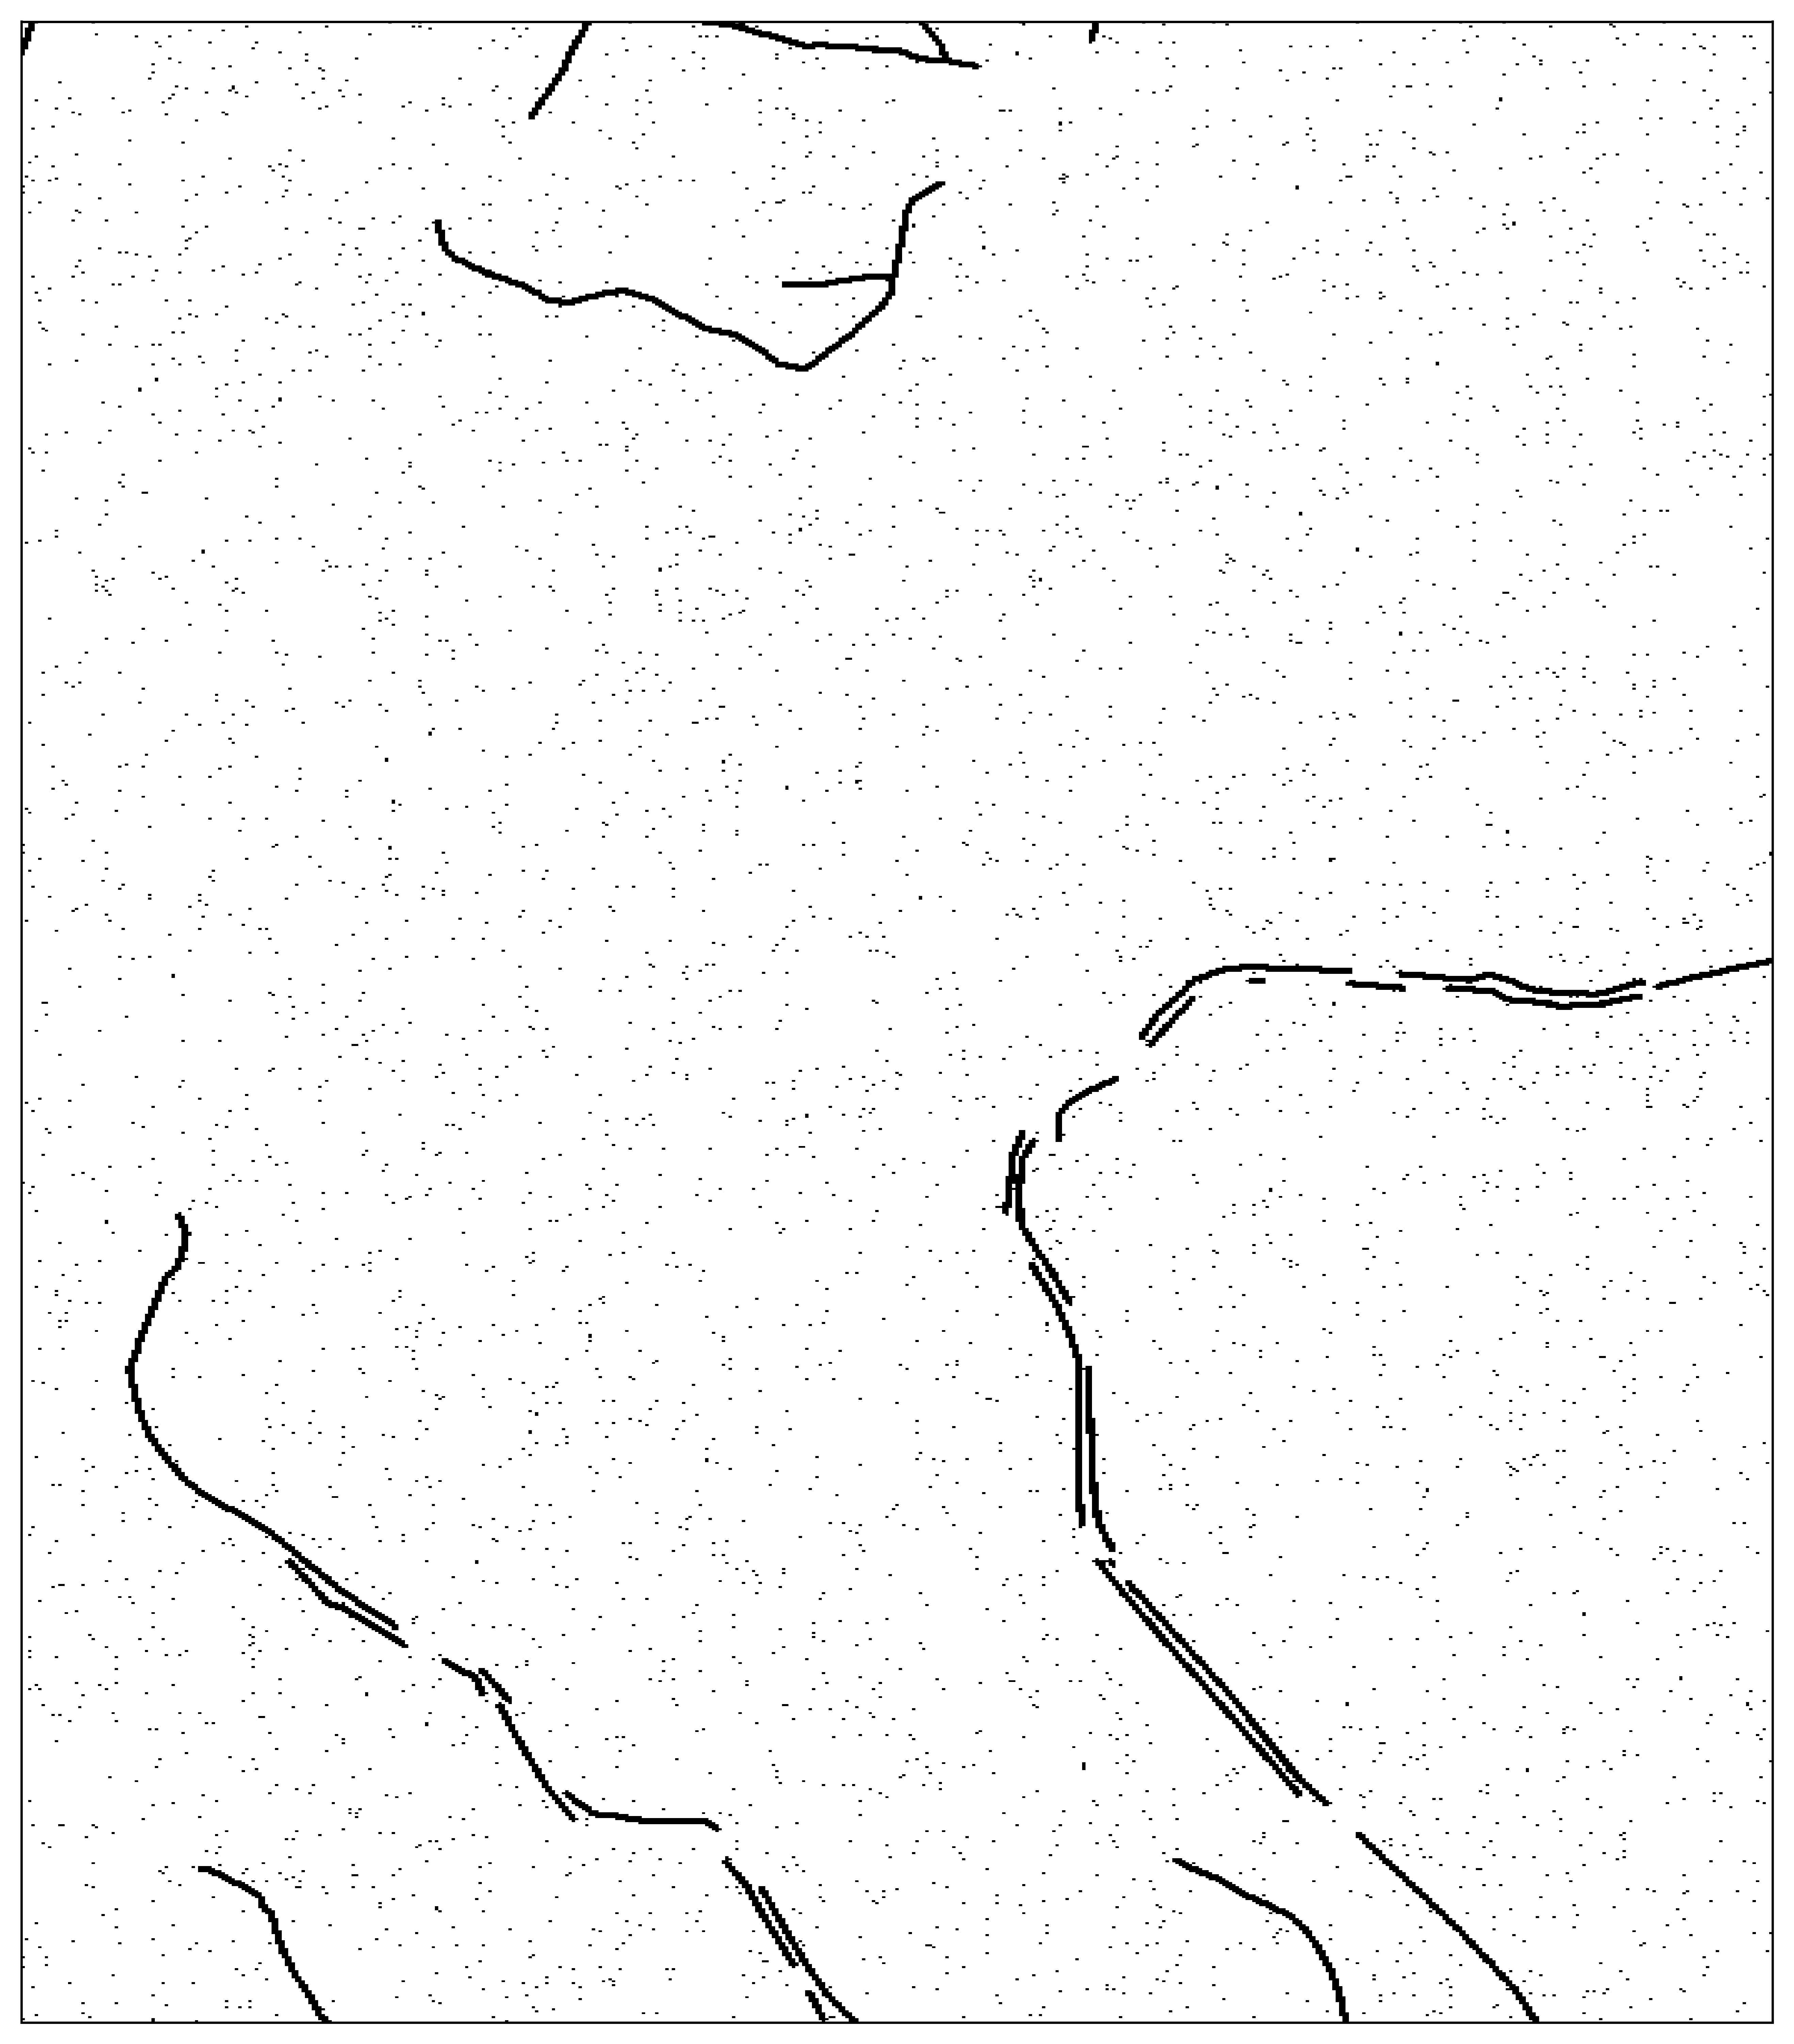
\includegraphics{./images/publ_balanced_masks_A_lo.jpg}}}%%%
\DIFdelFL{\hspace{5pt}
    }%DIFDELCMD < \subfigure[]{
%DIFDELCMD <         \resizebox*{6.85cm}{!}{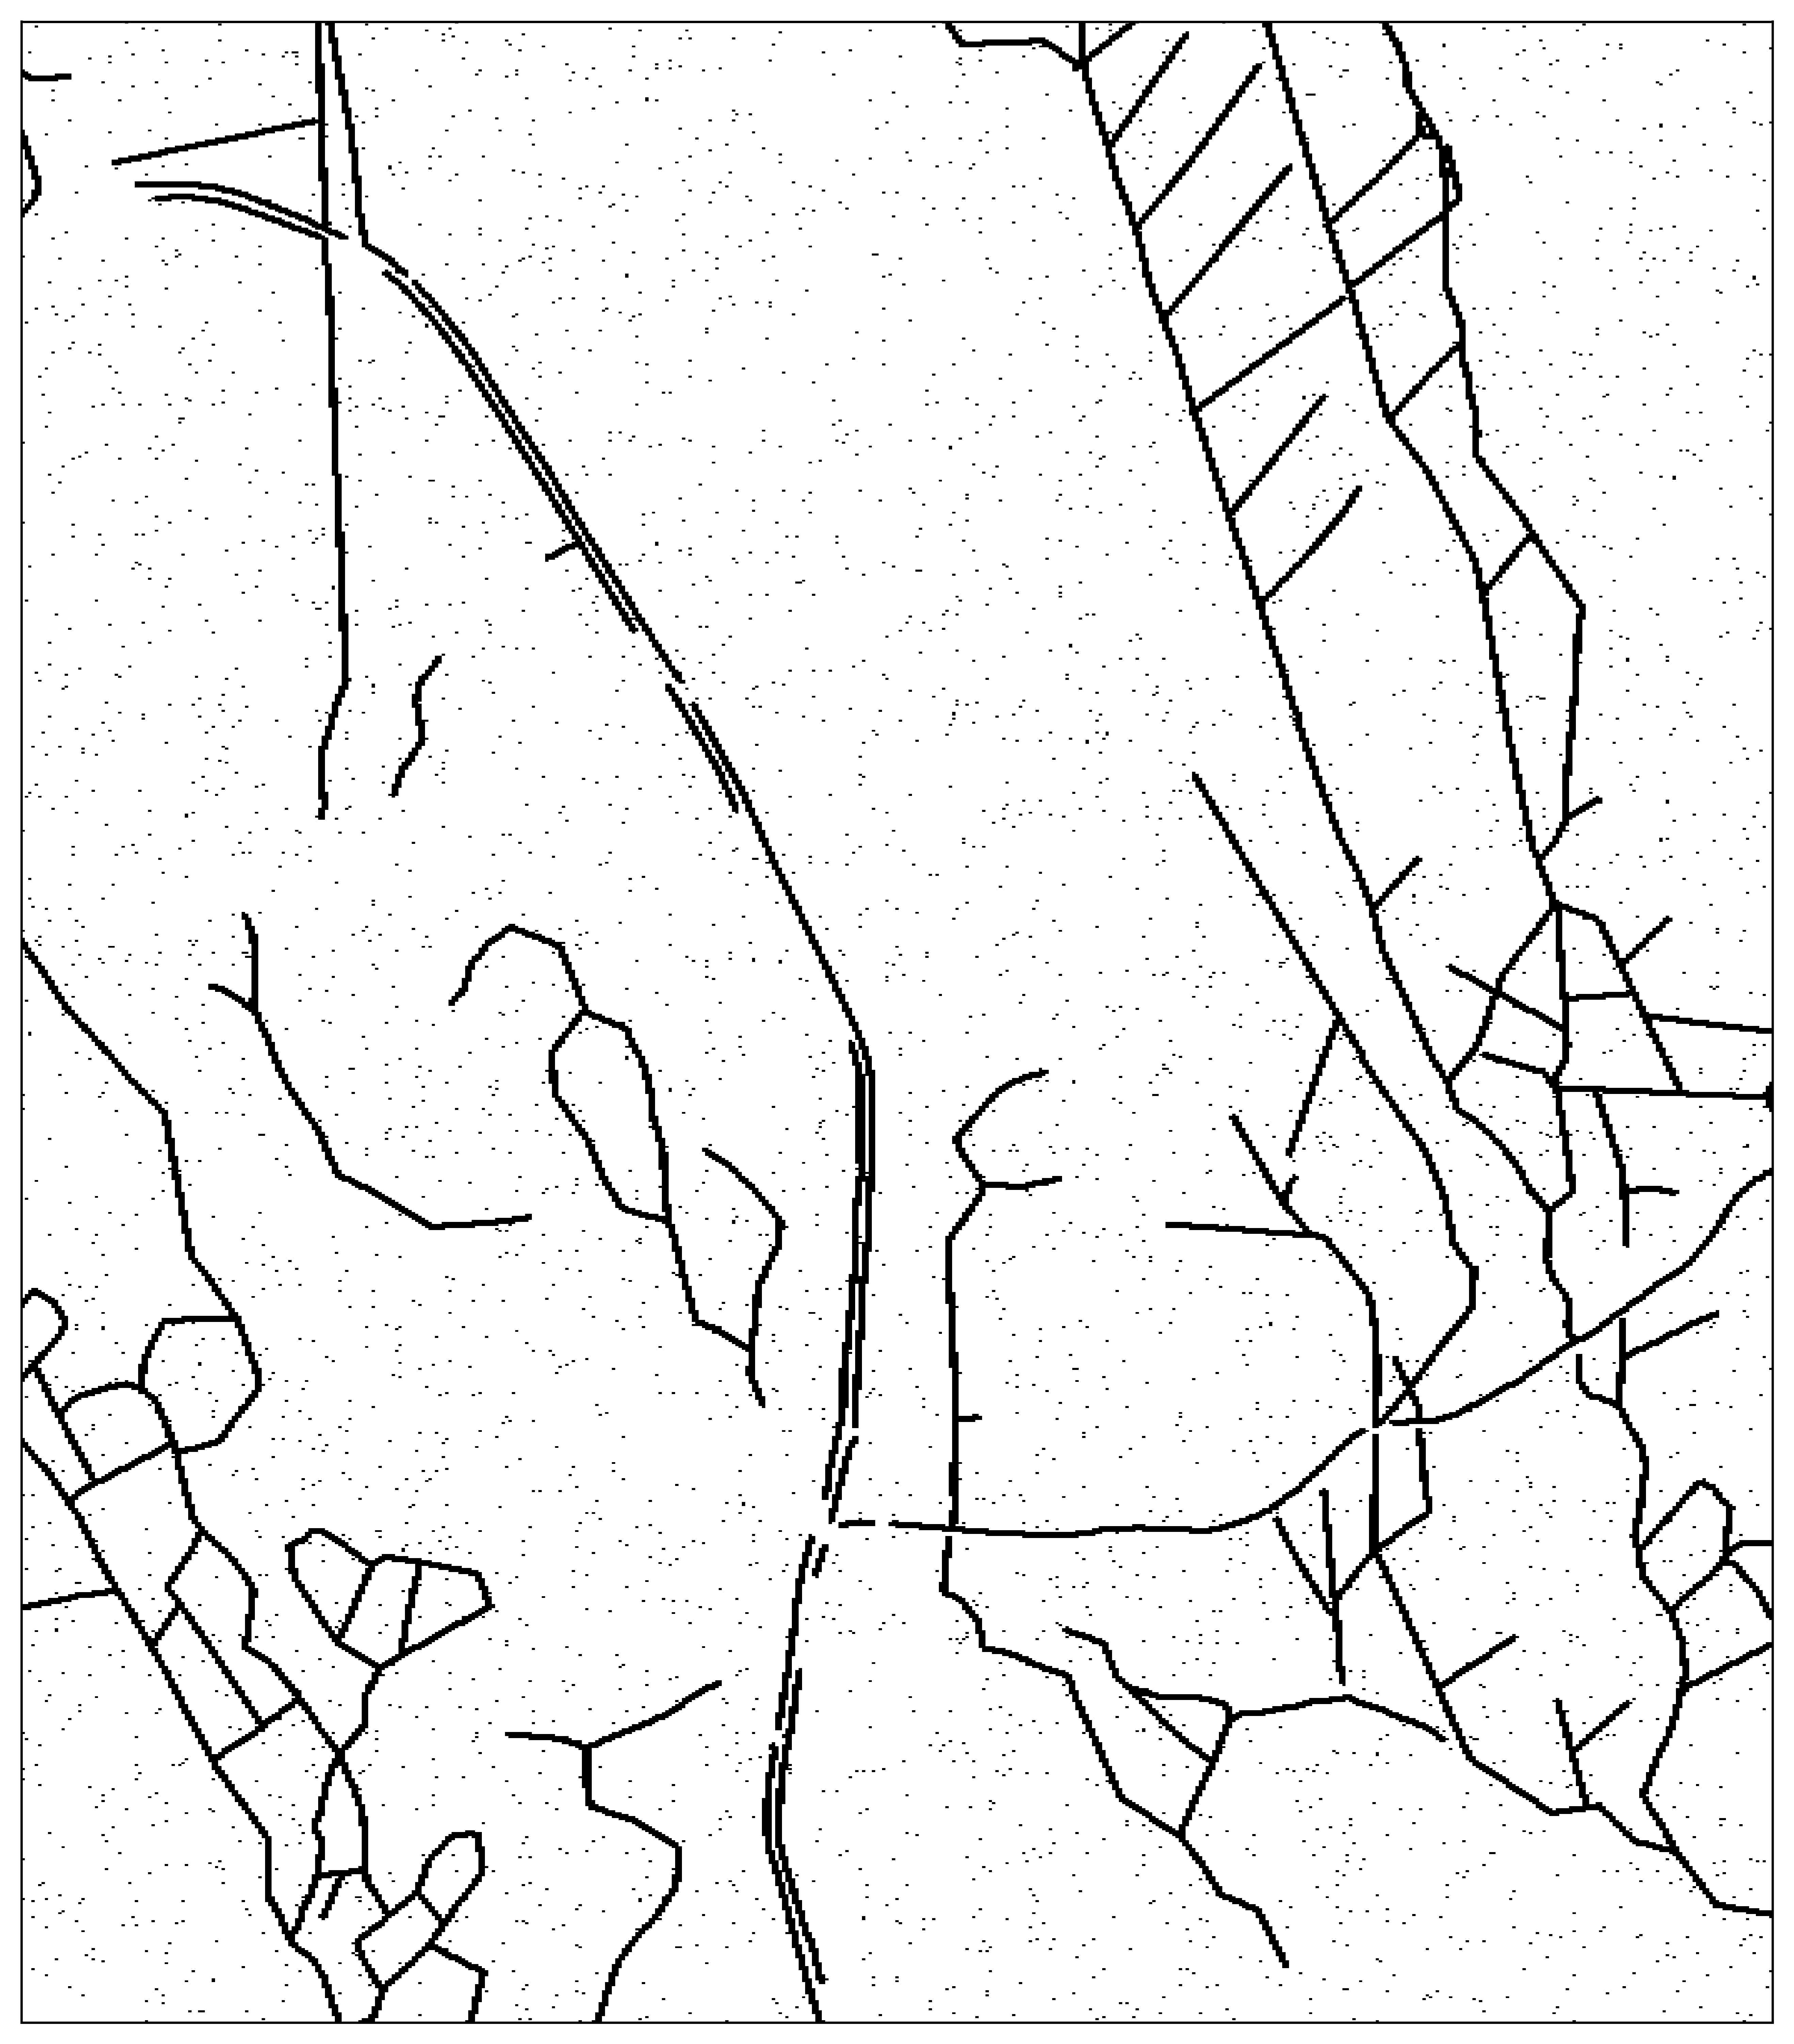
\includegraphics{./images/publ_balanced_masks_B_lo.jpg}}}
%DIFDELCMD <     %%%
\DIFdelendFL \DIFaddbeginFL \subfigure[]{
        \resizebox*{5.6cm}{!}{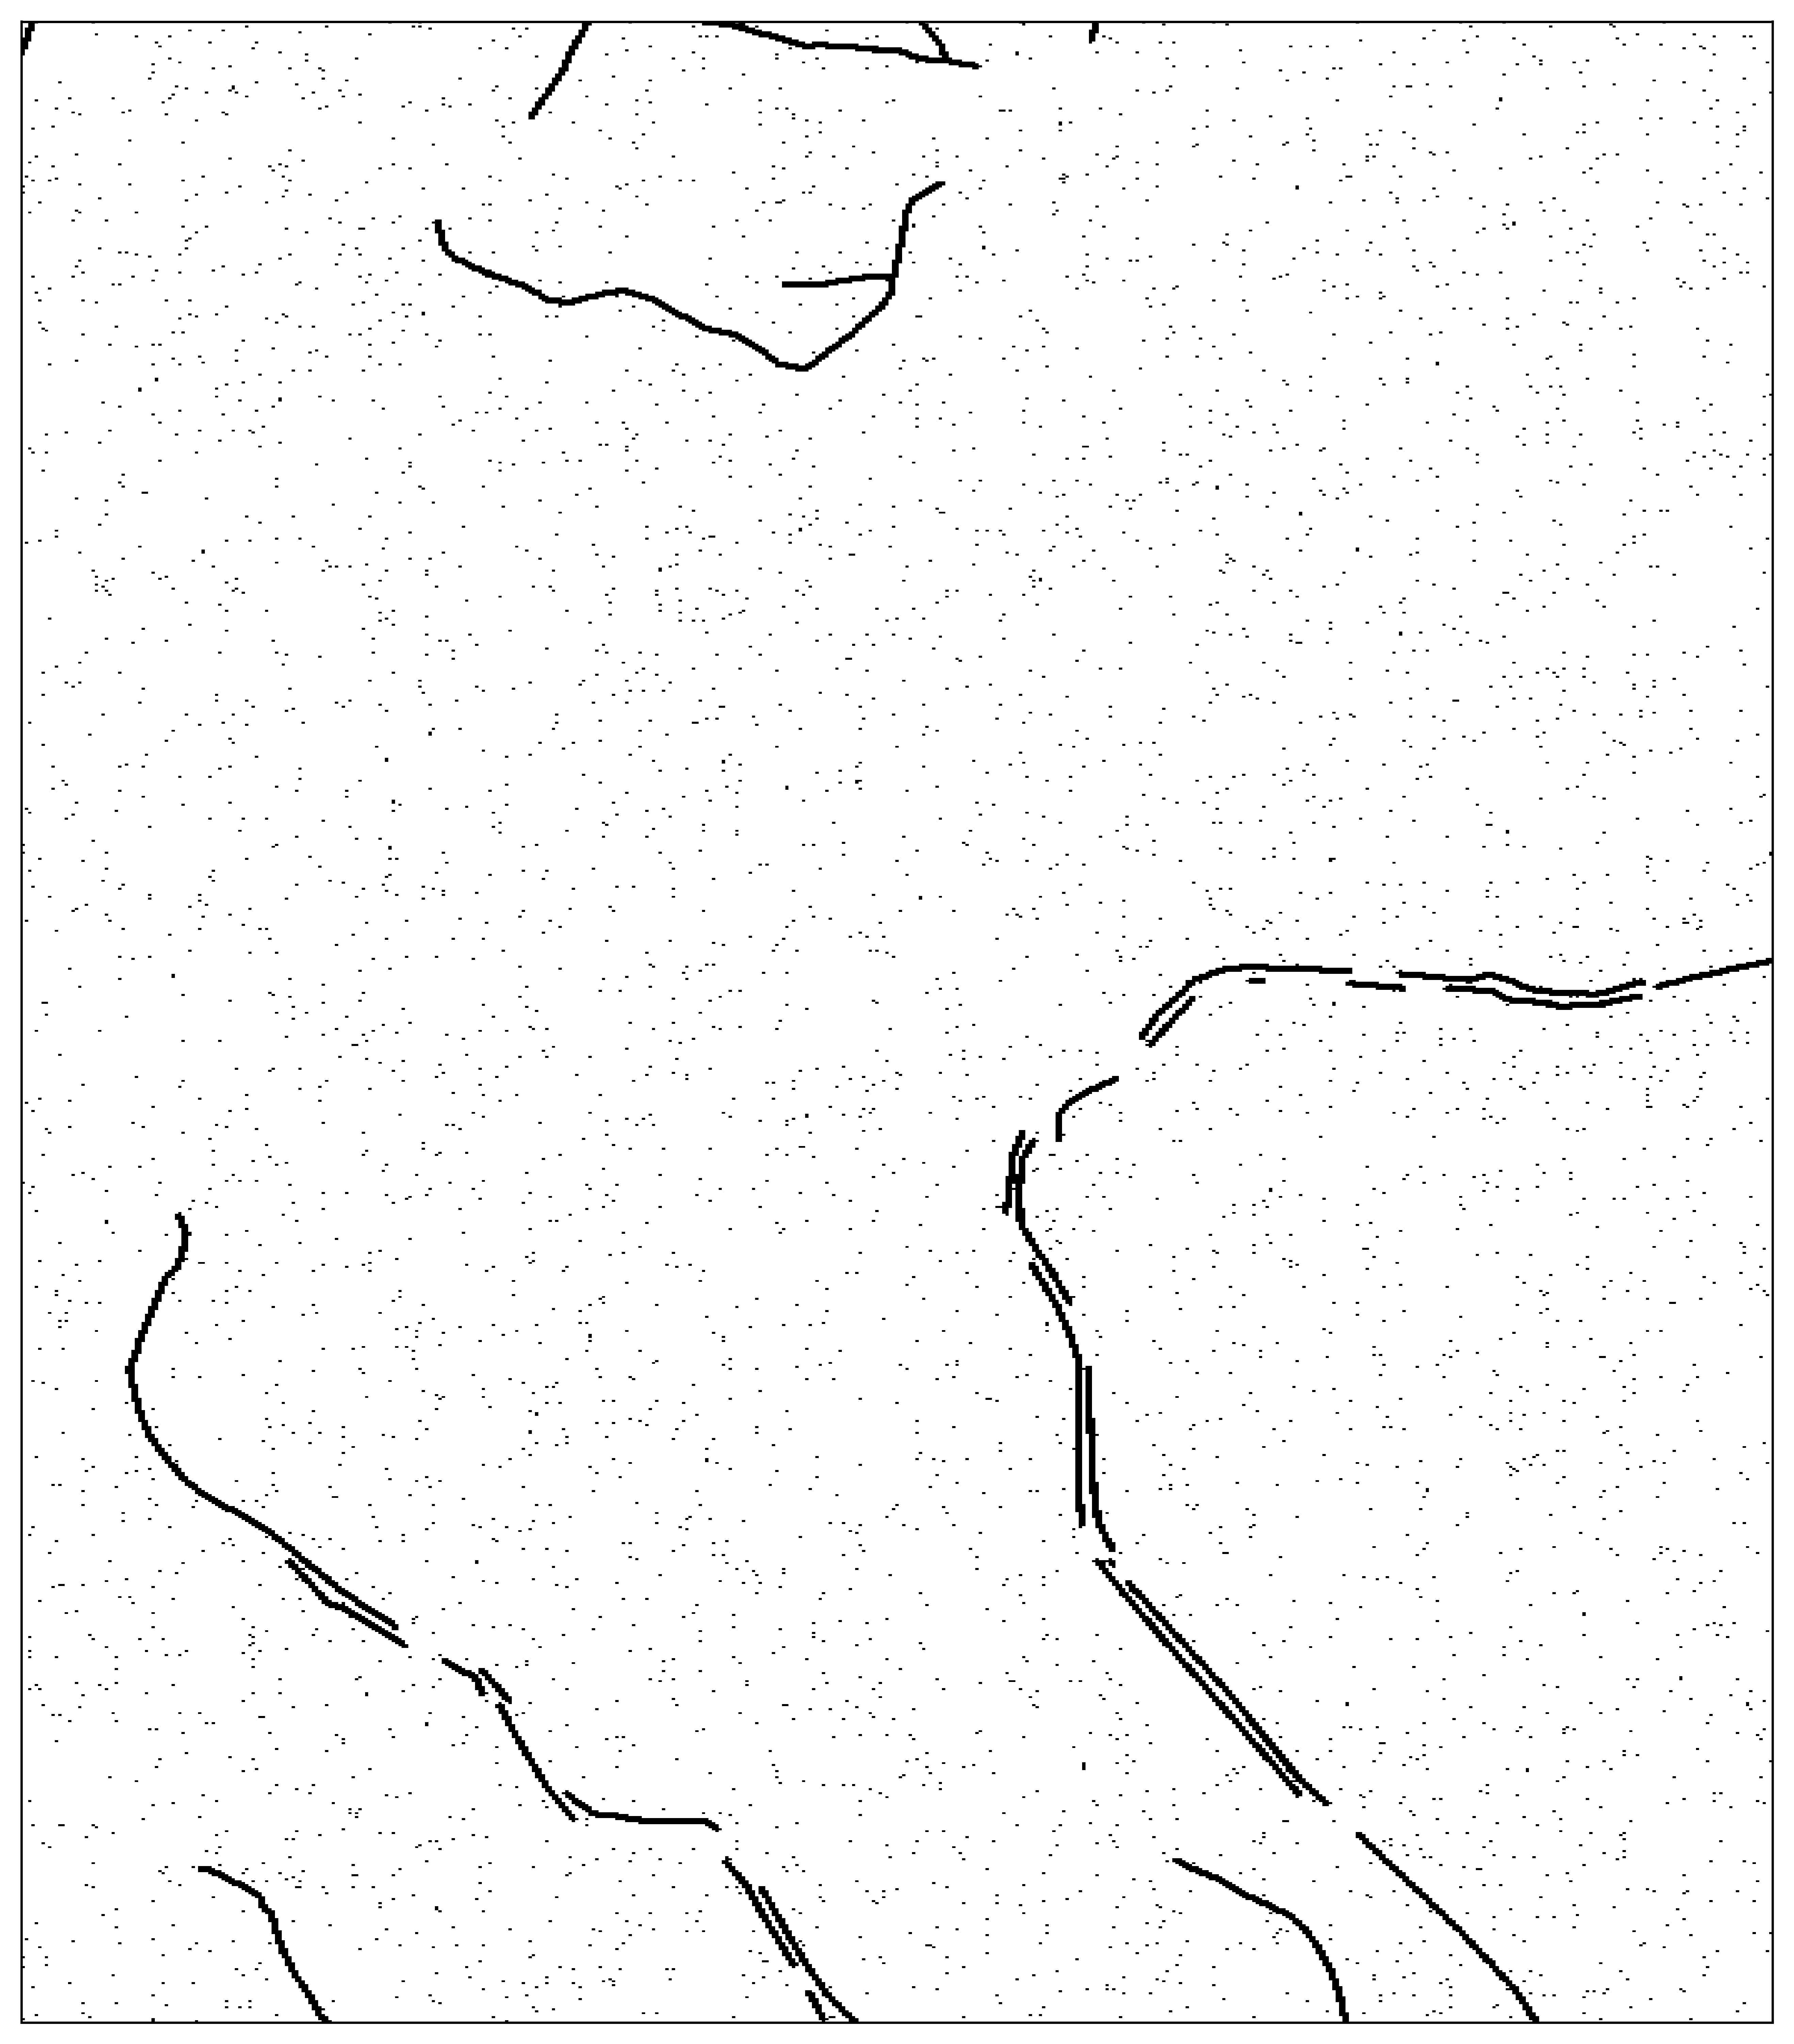
\includegraphics{./images/publ_balanced_masks_A_lo.jpg}}}\DIFaddFL{\hspace{5pt}
    }\subfigure[]{
        \resizebox*{5.6cm}{!}{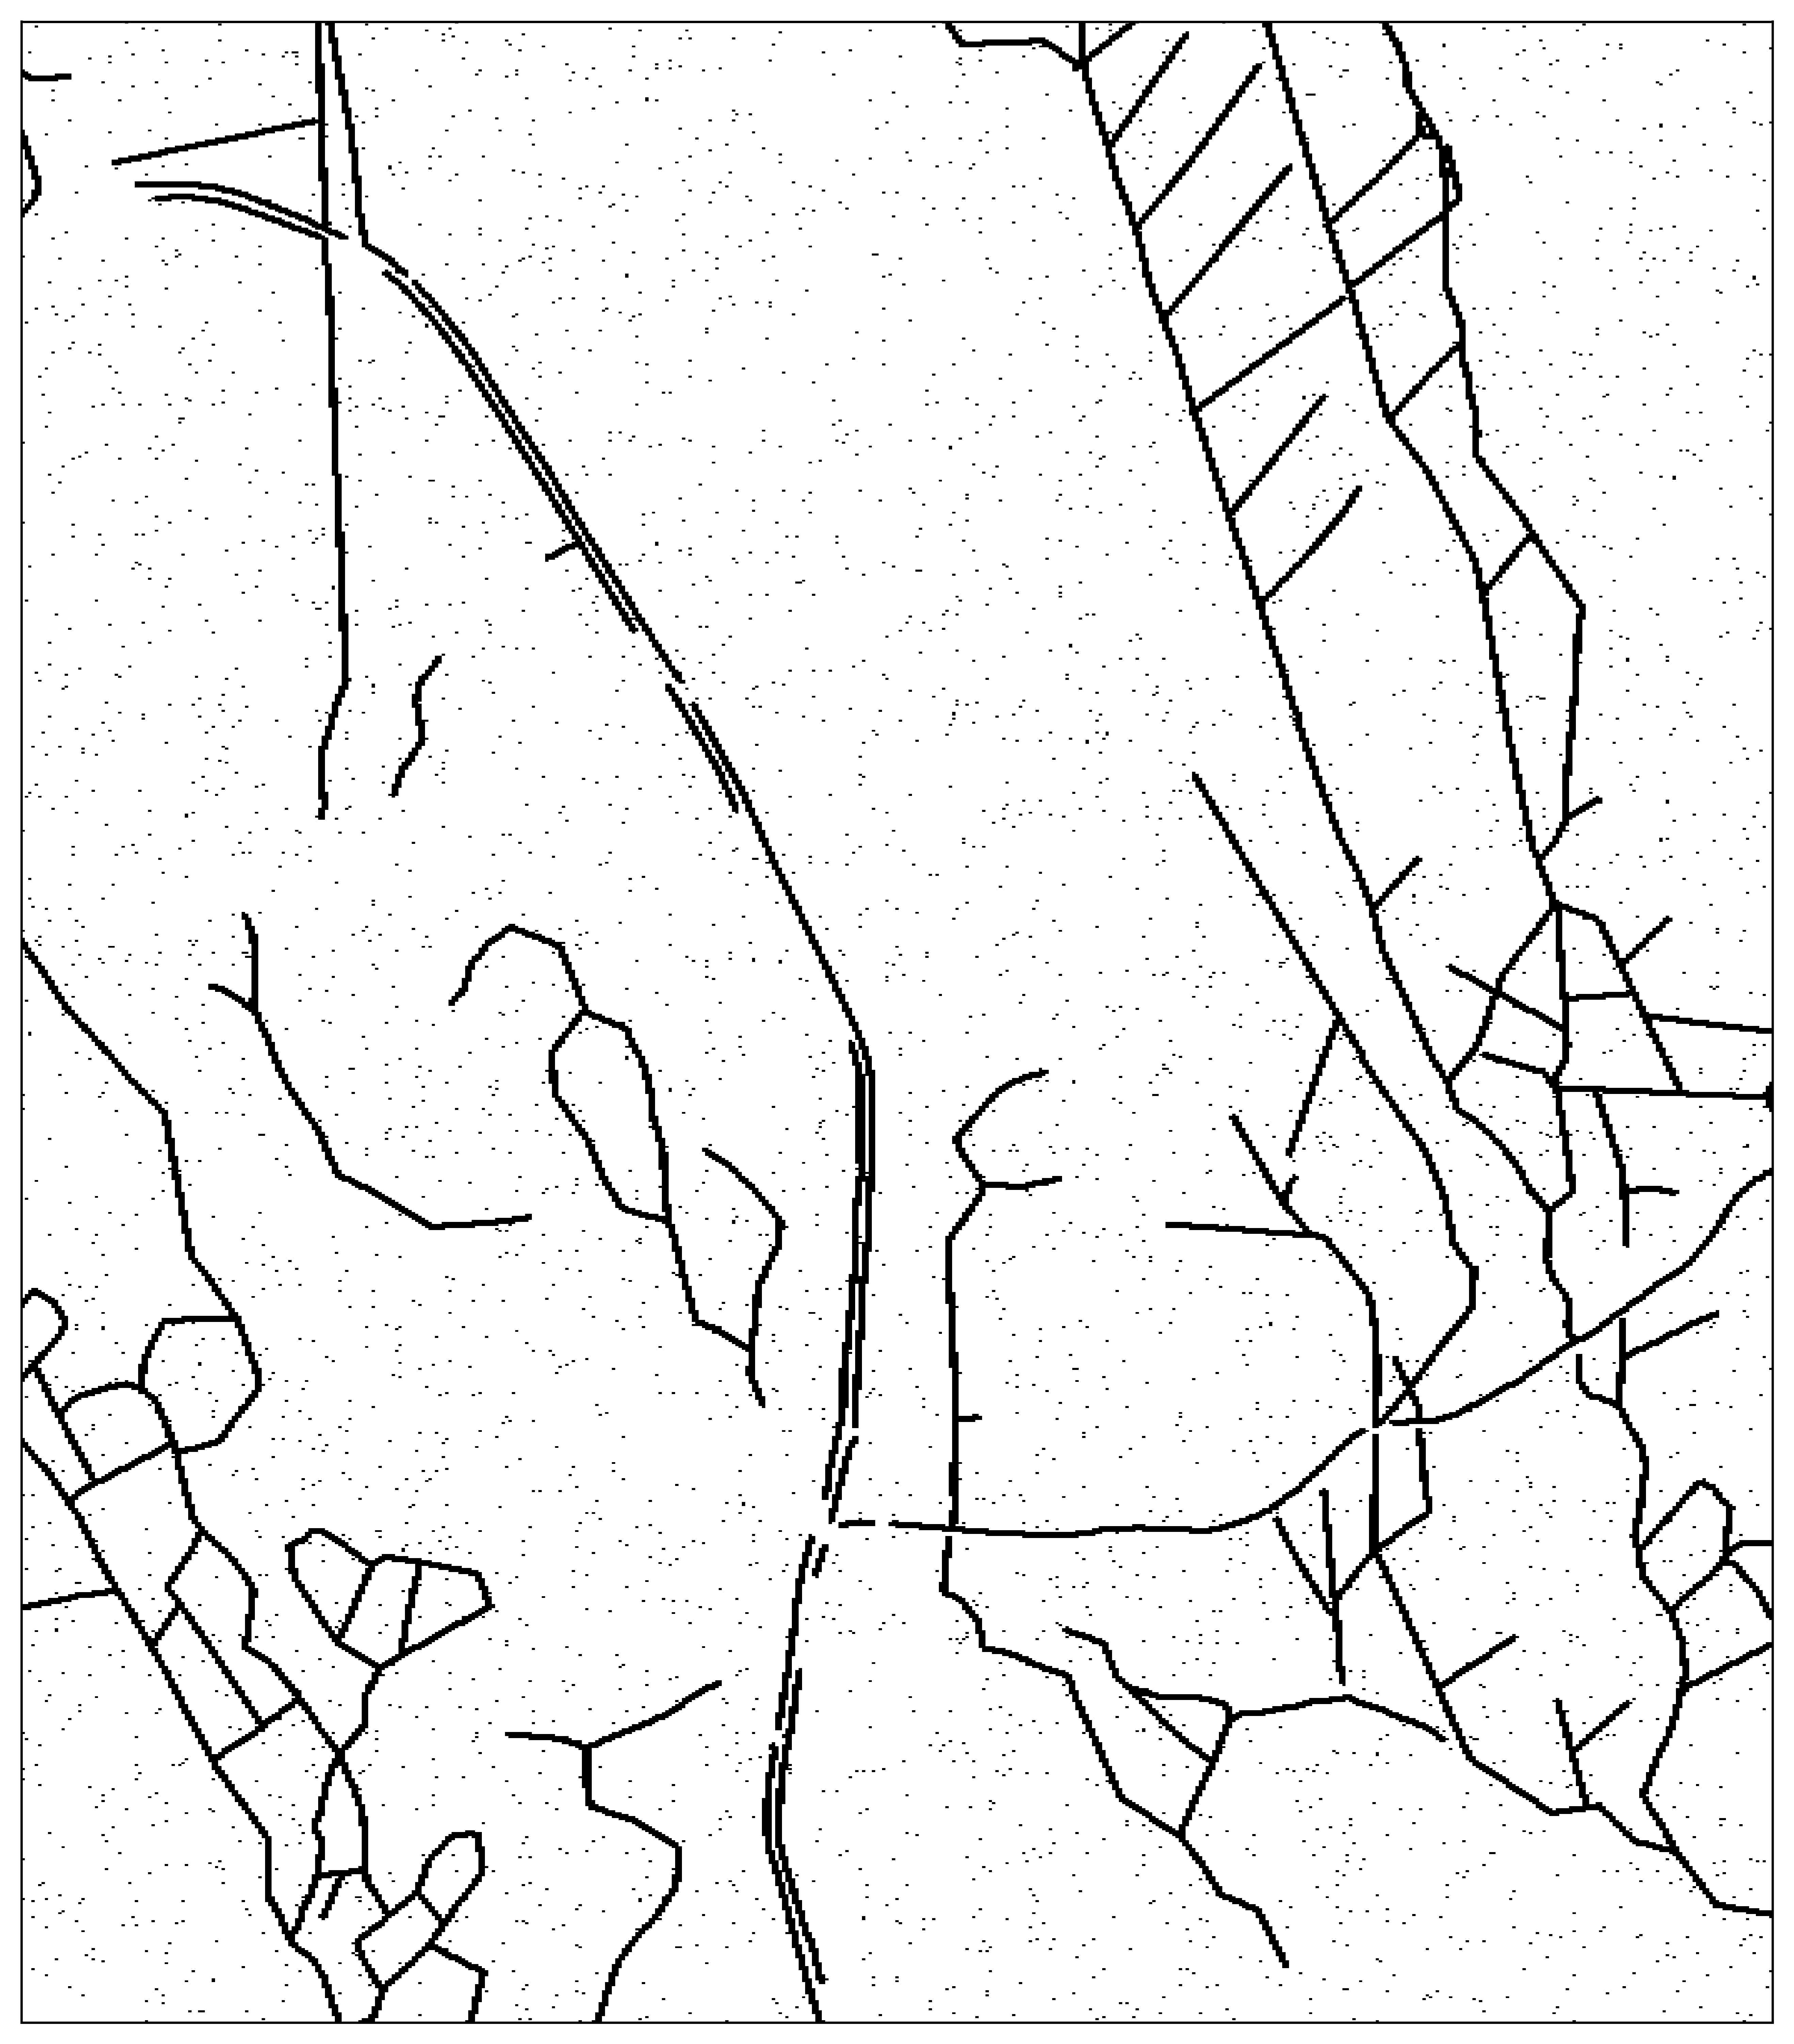
\includegraphics{./images/publ_balanced_masks_B_lo.jpg}}}
    \DIFaddendFL \caption{\DIFaddbeginFL \textbf{\DIFaddFL{Balancing training data.}} \DIFaddendFL Black pixels here indicate the balanced masks used to determine what pixels were used when training the models. \textbf{a, b: }Examples of two subsection from the training dataset.}
    \label{fig:balancedmasks}
\end{figure}

\DIFaddbegin \newpage
\DIFaddend \subsection{Post-processing}
\DIFdelbegin \DIFdel{The models output a ditch class probability prediction for each pixel. Values close to zero indicate a low probability of a pixel lying in a ditch, whereas values close to one equals a high ditch probability }\DIFdelend \DIFaddbegin 

\DIFadd{The output from the model is a ditch probability ranging from zero to one for each pixel }\DIFaddend (\hyperref[fig:postprocessing1]{Figure} \ref{fig:postprocessing1} \hyperref[fig:postprocessing1]{a}).

\subsubsection{Noise reduction and gap filling}

The probability predictions contained a lot of noise in the areas largely distant from the ditches. This noise was removed by first using a bilateral de-noising filter, and then removing outlier pixels that were far away from any other high probability ditch pixels. This left linear properties and pixels with a very high value intact, while lowering the value of pixels that did not contribute to an accurate prediction (\hyperref[fig:postprocessing1]{Figure} \ref{fig:postprocessing1} \hyperref[fig:postprocessing1]{b}) (\hyperref[fig:postprocessing2]{Figure} \ref{fig:postprocessing2} \hyperref[fig:postprocessing2]{a}).

To fill gaps in ditches that the \DIFdelbegin \DIFdel{models }\DIFdelend \DIFaddbegin \DIFadd{model }\DIFaddend failed to correctly predict \DIFaddbegin \DIFadd{due to gaps in the LiDAR scans}\DIFaddend , we aggregated pixel values by covering them with cone masks expanding outwards in different directions from the examined pixel. This amplified some of the noise that was left, but filling the gaps in the ditches was judged to be more important (\hyperref[fig:postprocessing2]{Figure} \ref{fig:postprocessing2} \hyperref[fig:postprocessing2]{b}).

\begin{figure} [!htb]
    \centering
    \DIFdelbeginFL %DIFDELCMD < \subfigure[]{
%DIFDELCMD <         \resizebox*{6.85cm}{!}{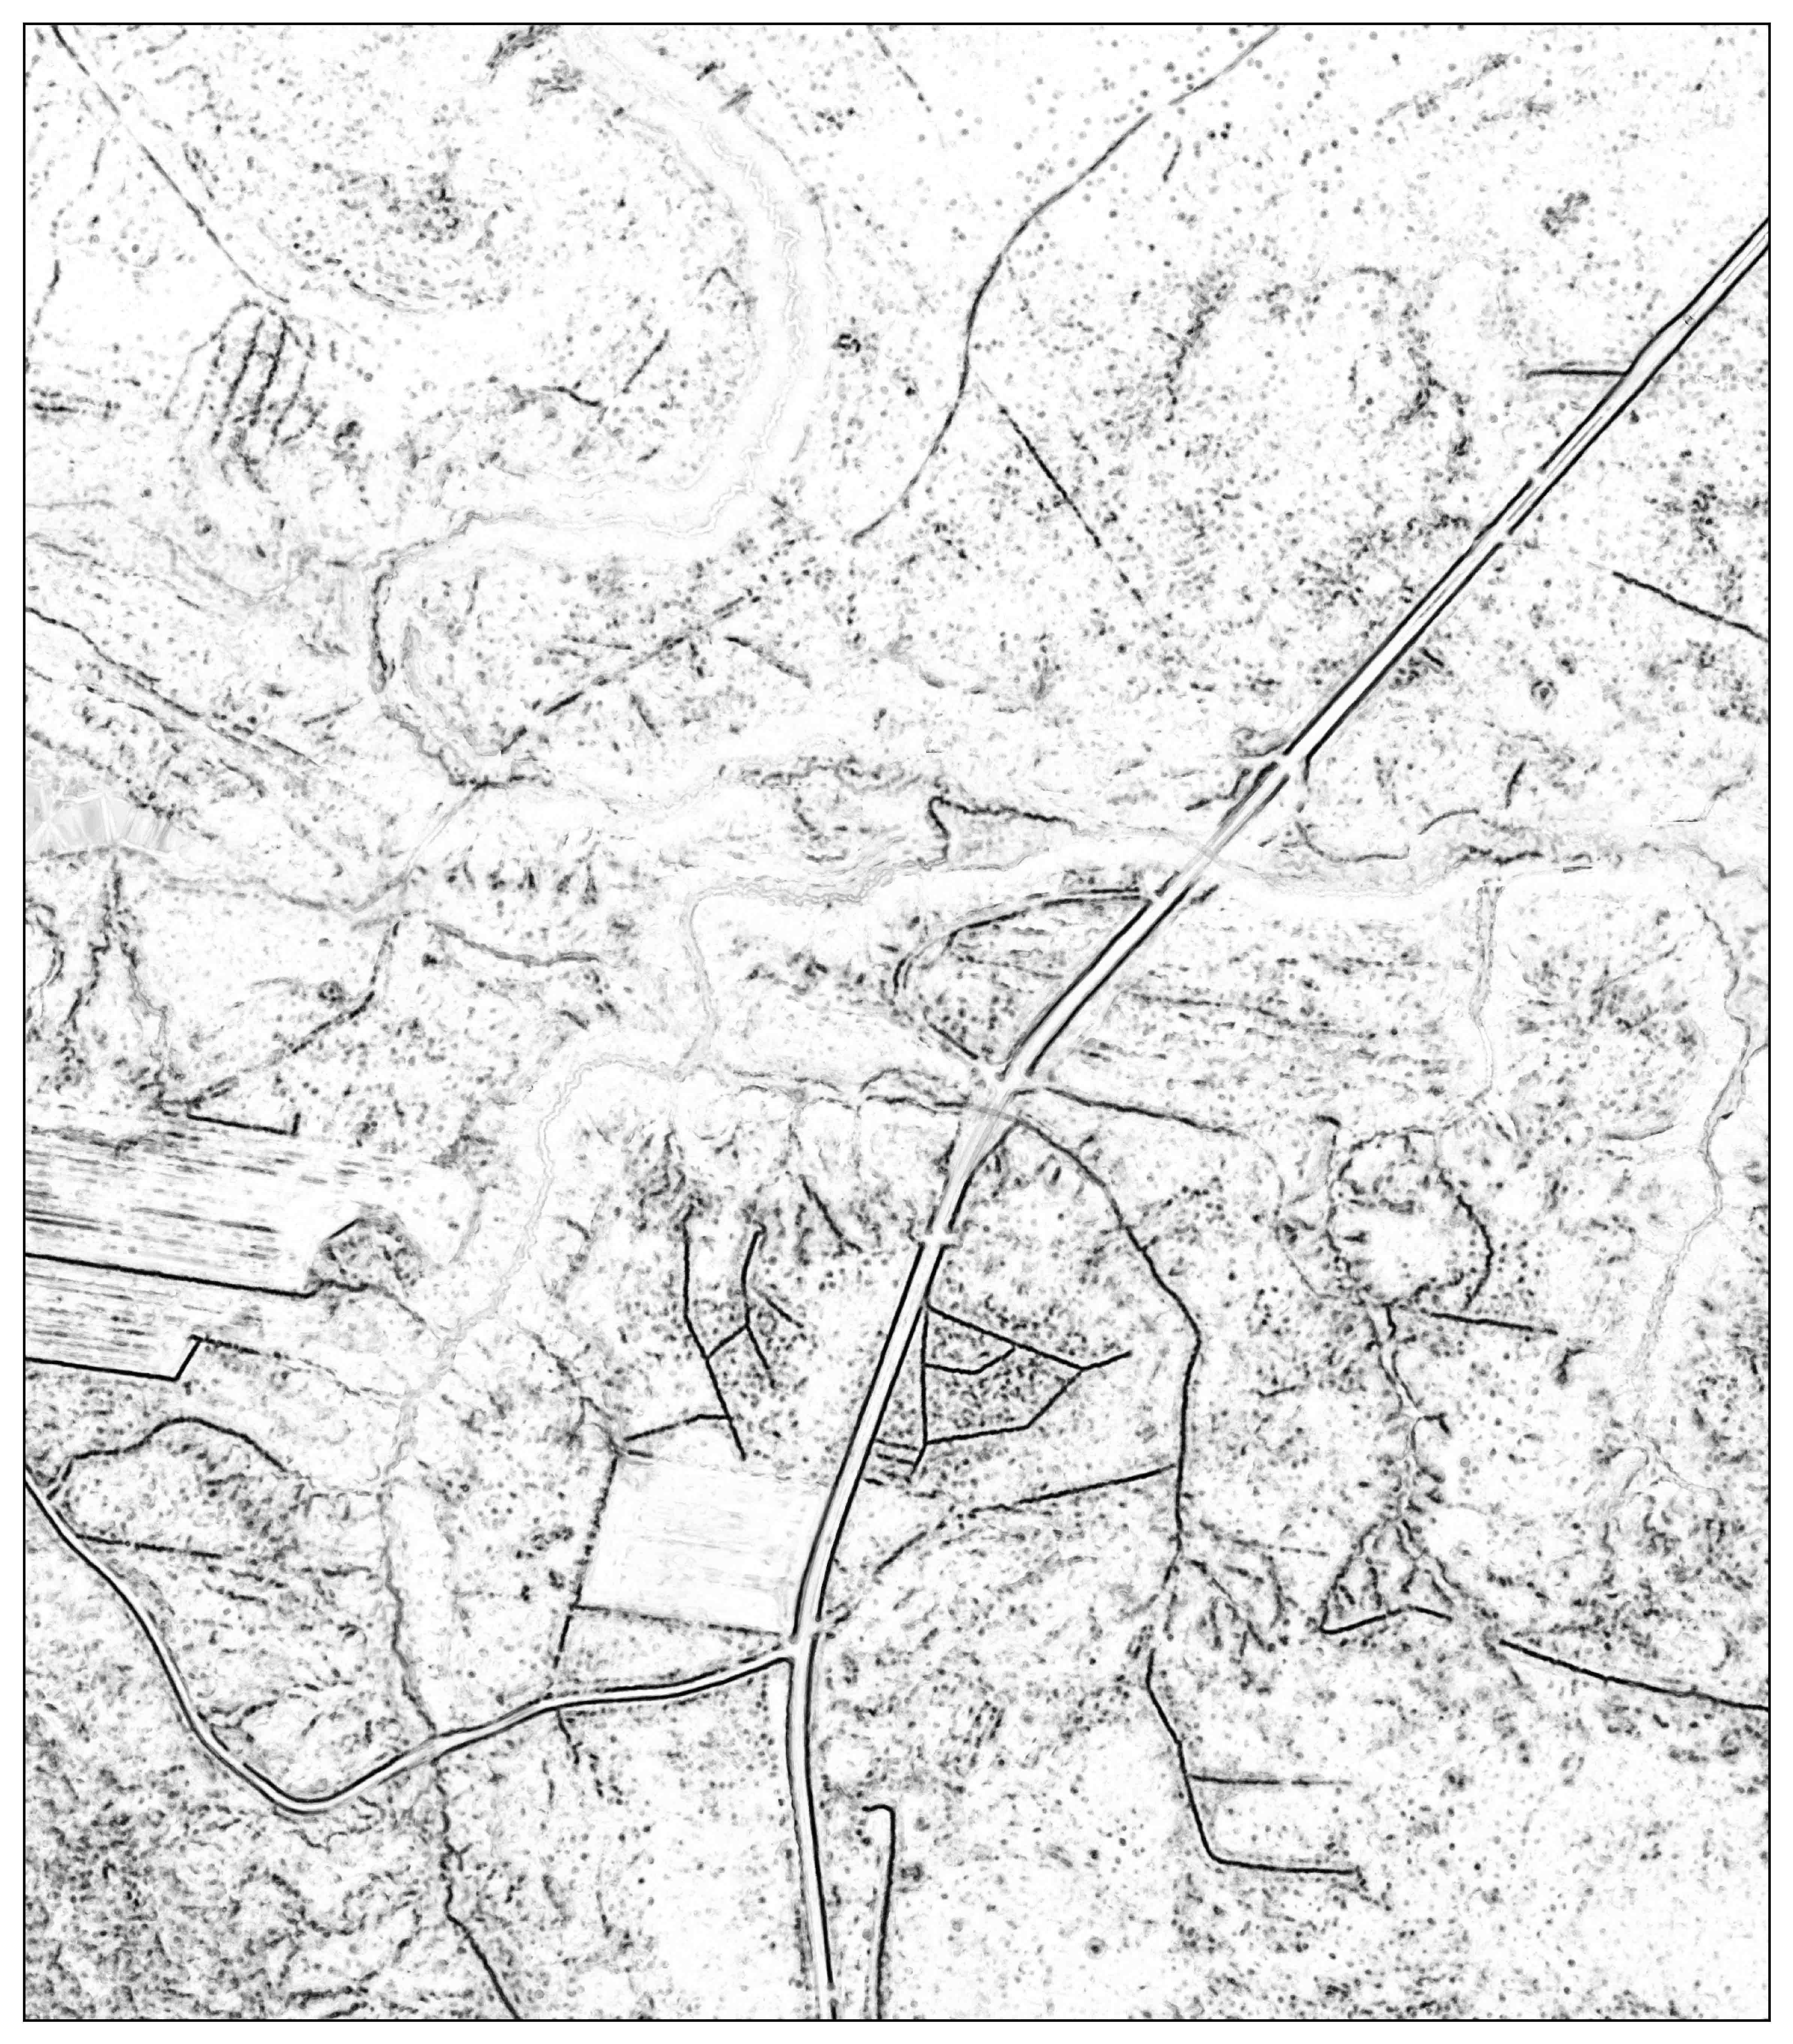
\includegraphics{./images/publ_post_process_step_1_lo.jpg}}}%%%
\DIFdelFL{\hspace{5pt}
    }%DIFDELCMD < \subfigure[]{
%DIFDELCMD <         \resizebox*{6.85cm}{!}{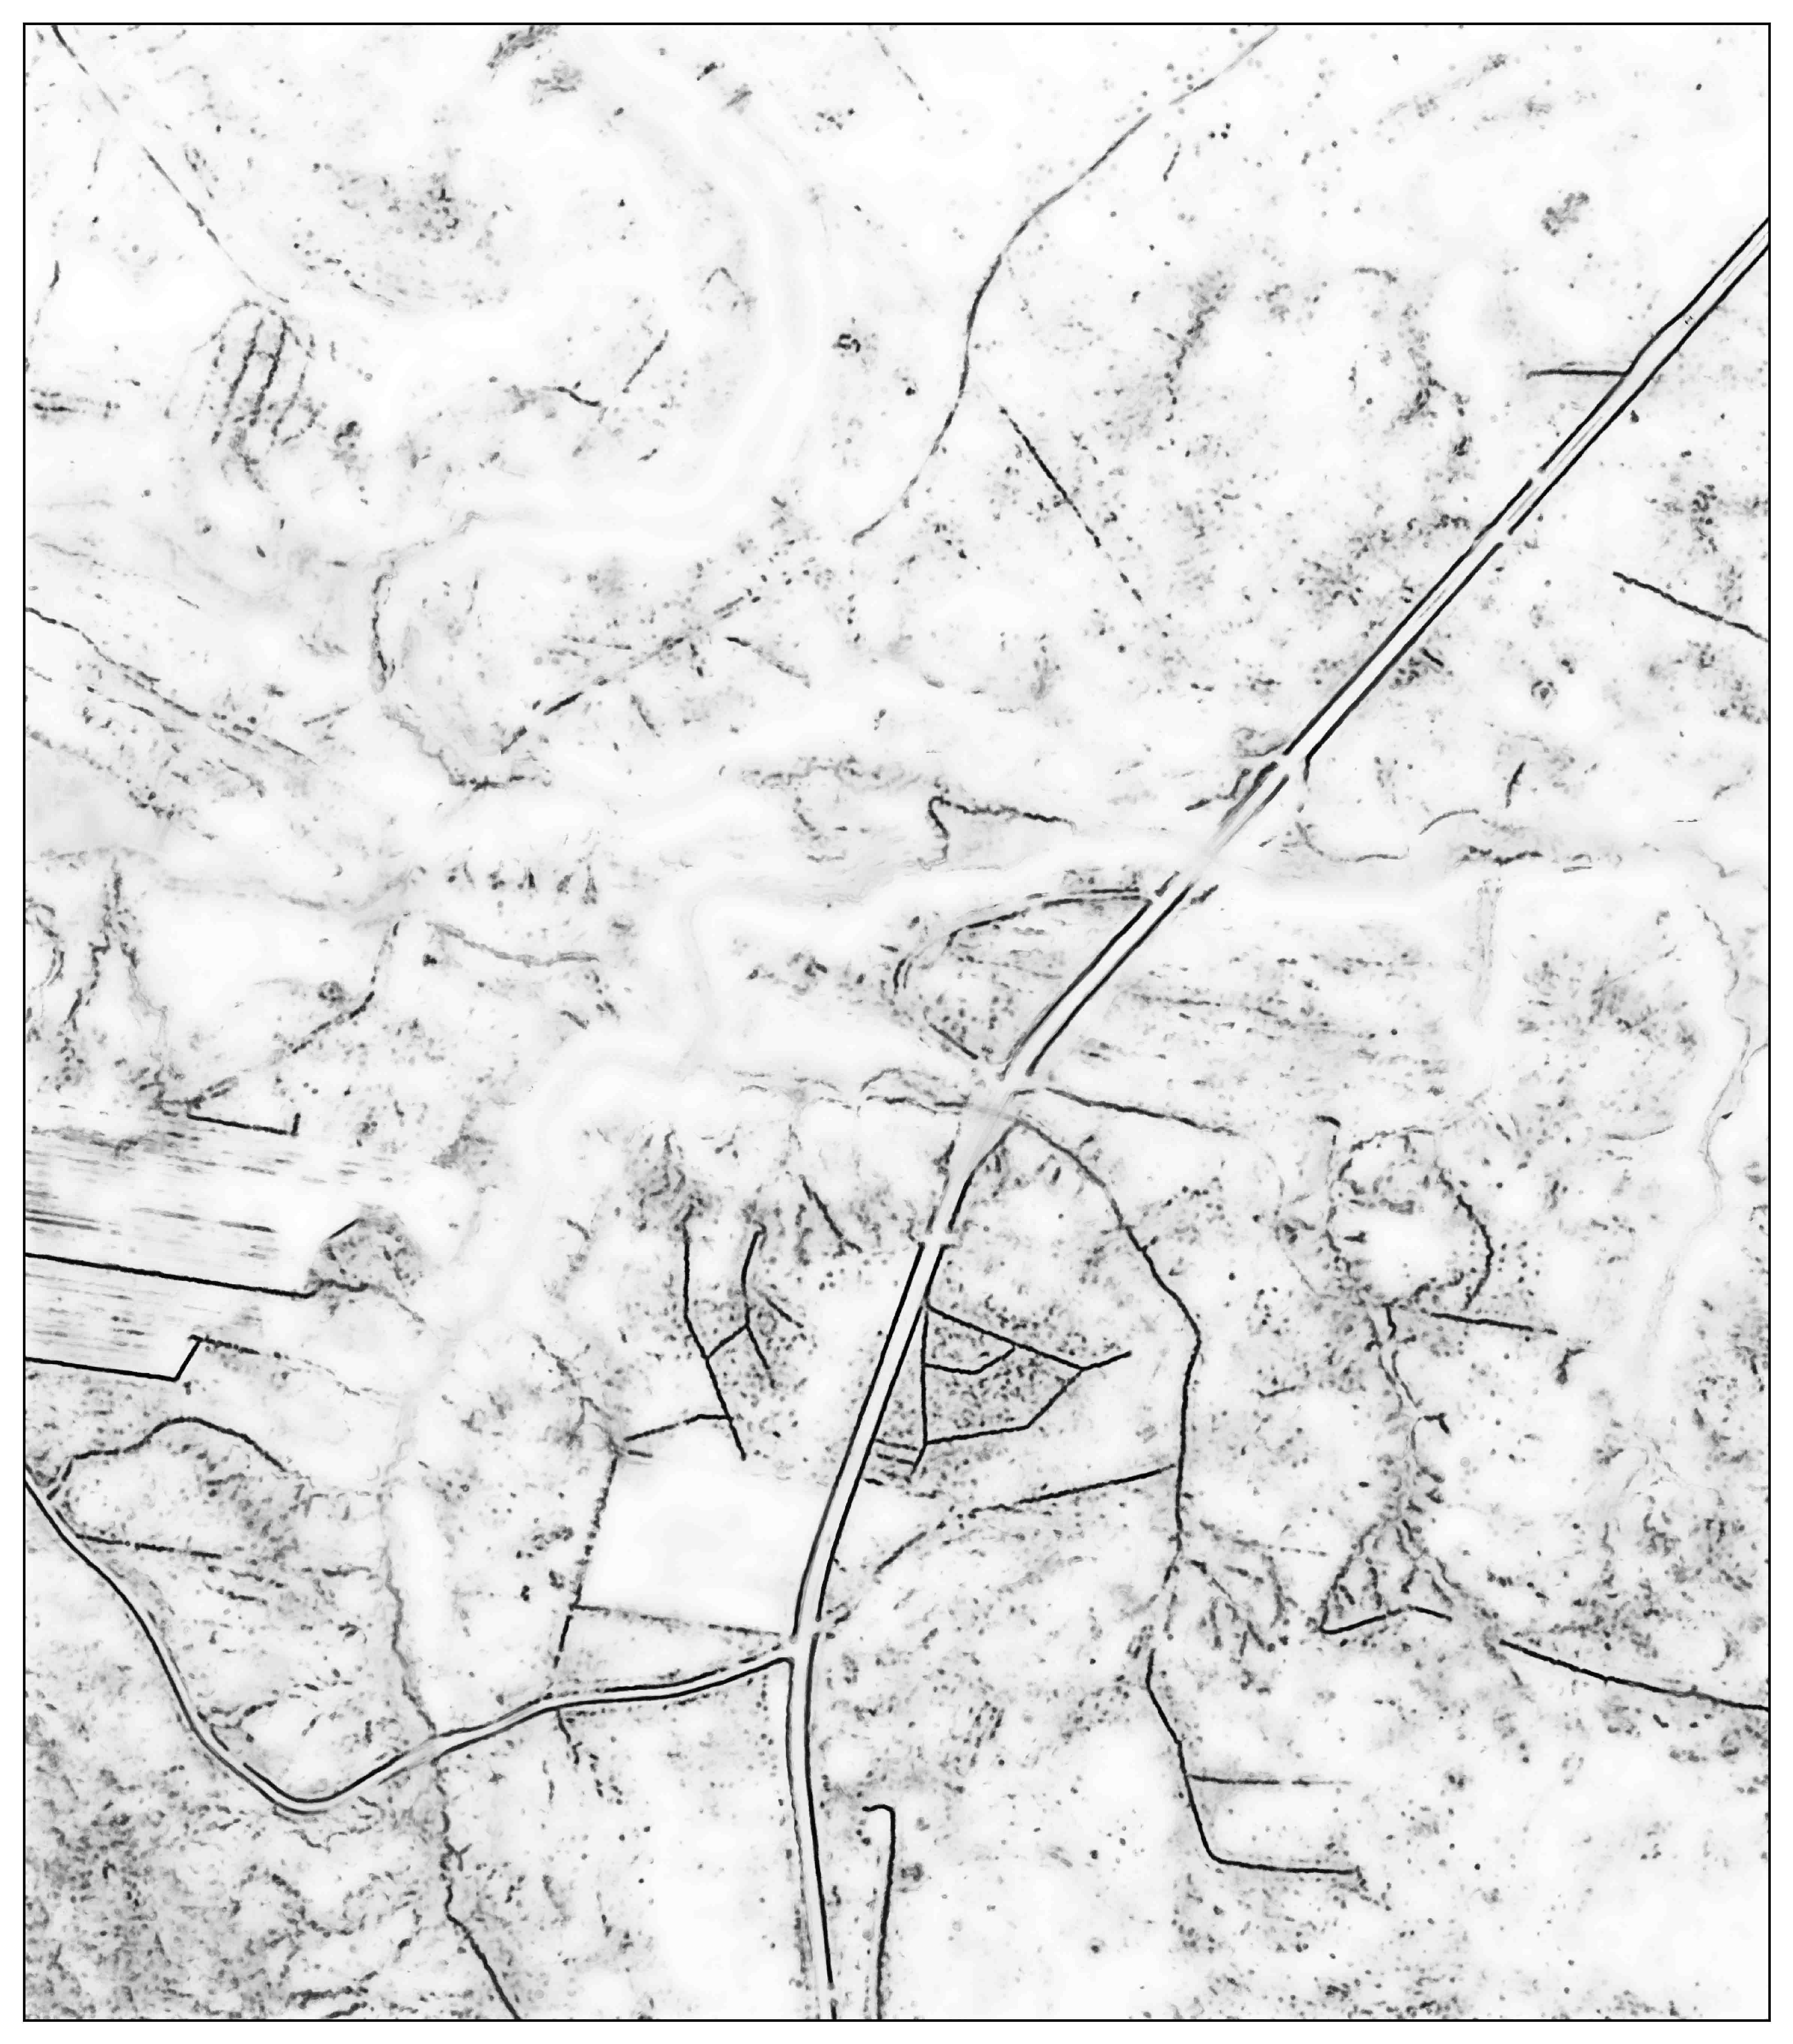
\includegraphics{./images/publ_post_process_step_2_lo.jpg}}}
%DIFDELCMD <     %%%
\DIFdelendFL \DIFaddbeginFL \subfigure[]{
        \resizebox*{5.6cm}{!}{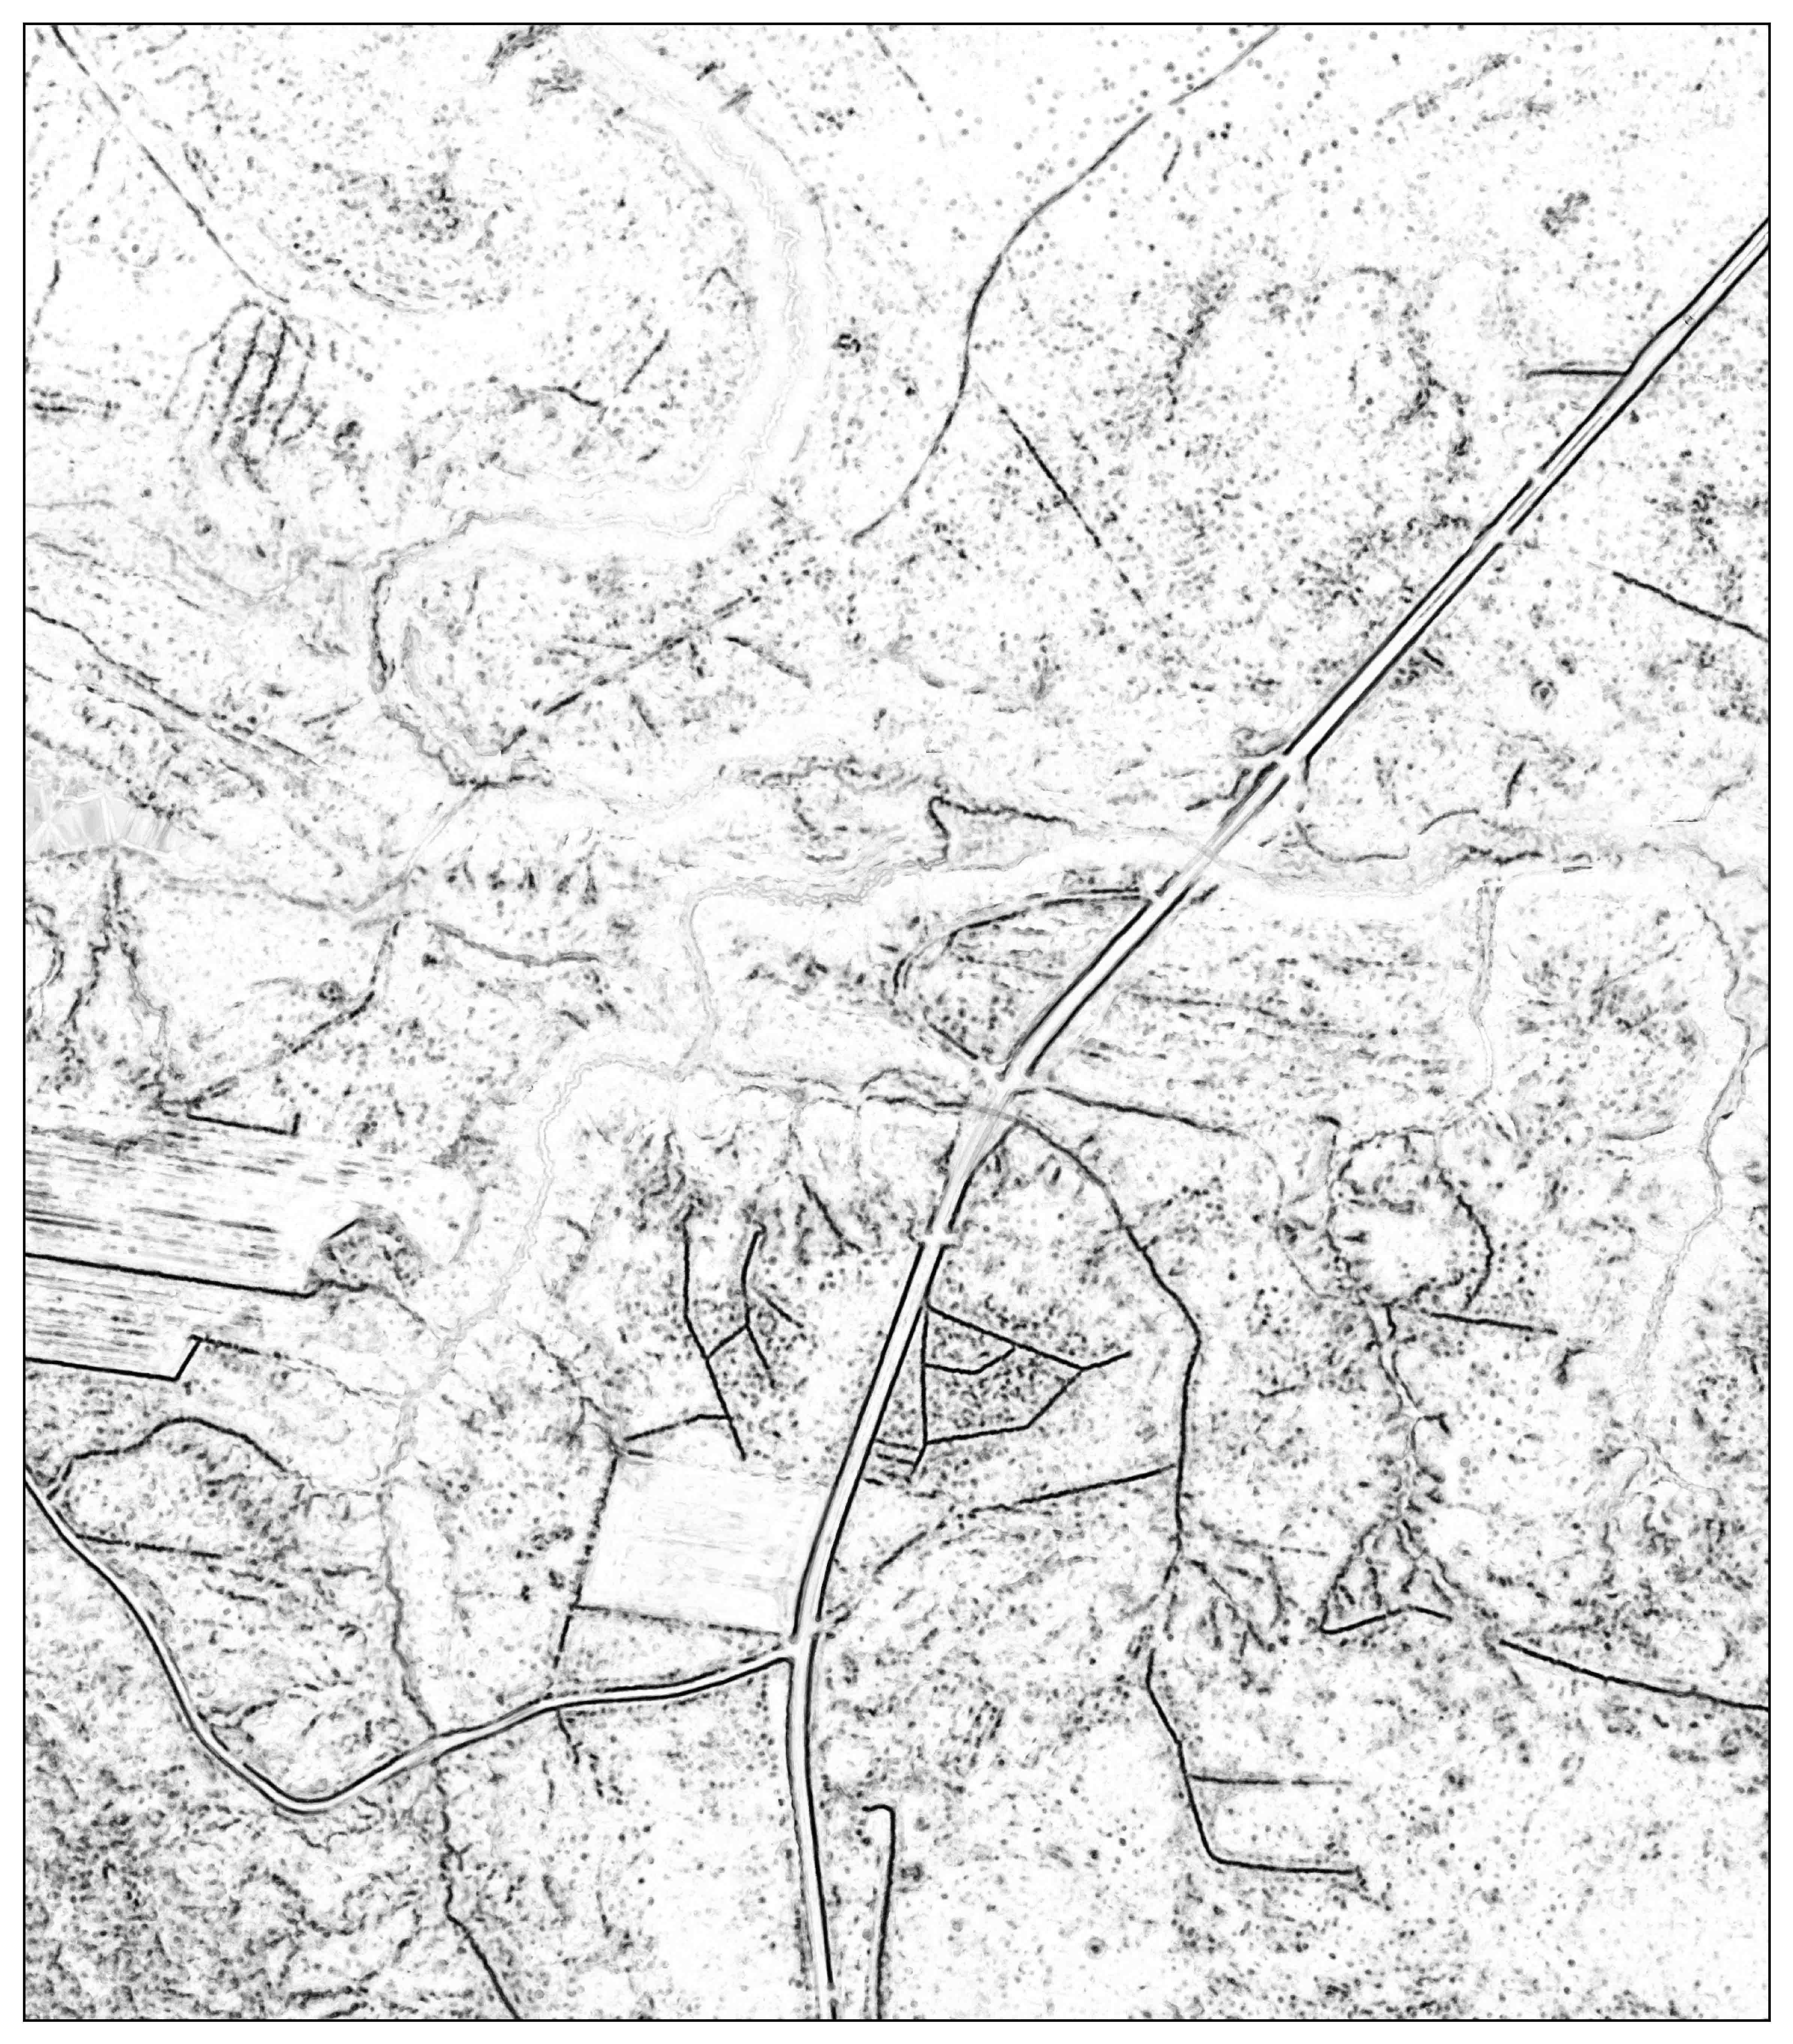
\includegraphics{./images/publ_post_process_step_1_lo.jpg}}}\DIFaddFL{\hspace{5pt}
    }\subfigure[]{
        \resizebox*{5.6cm}{!}{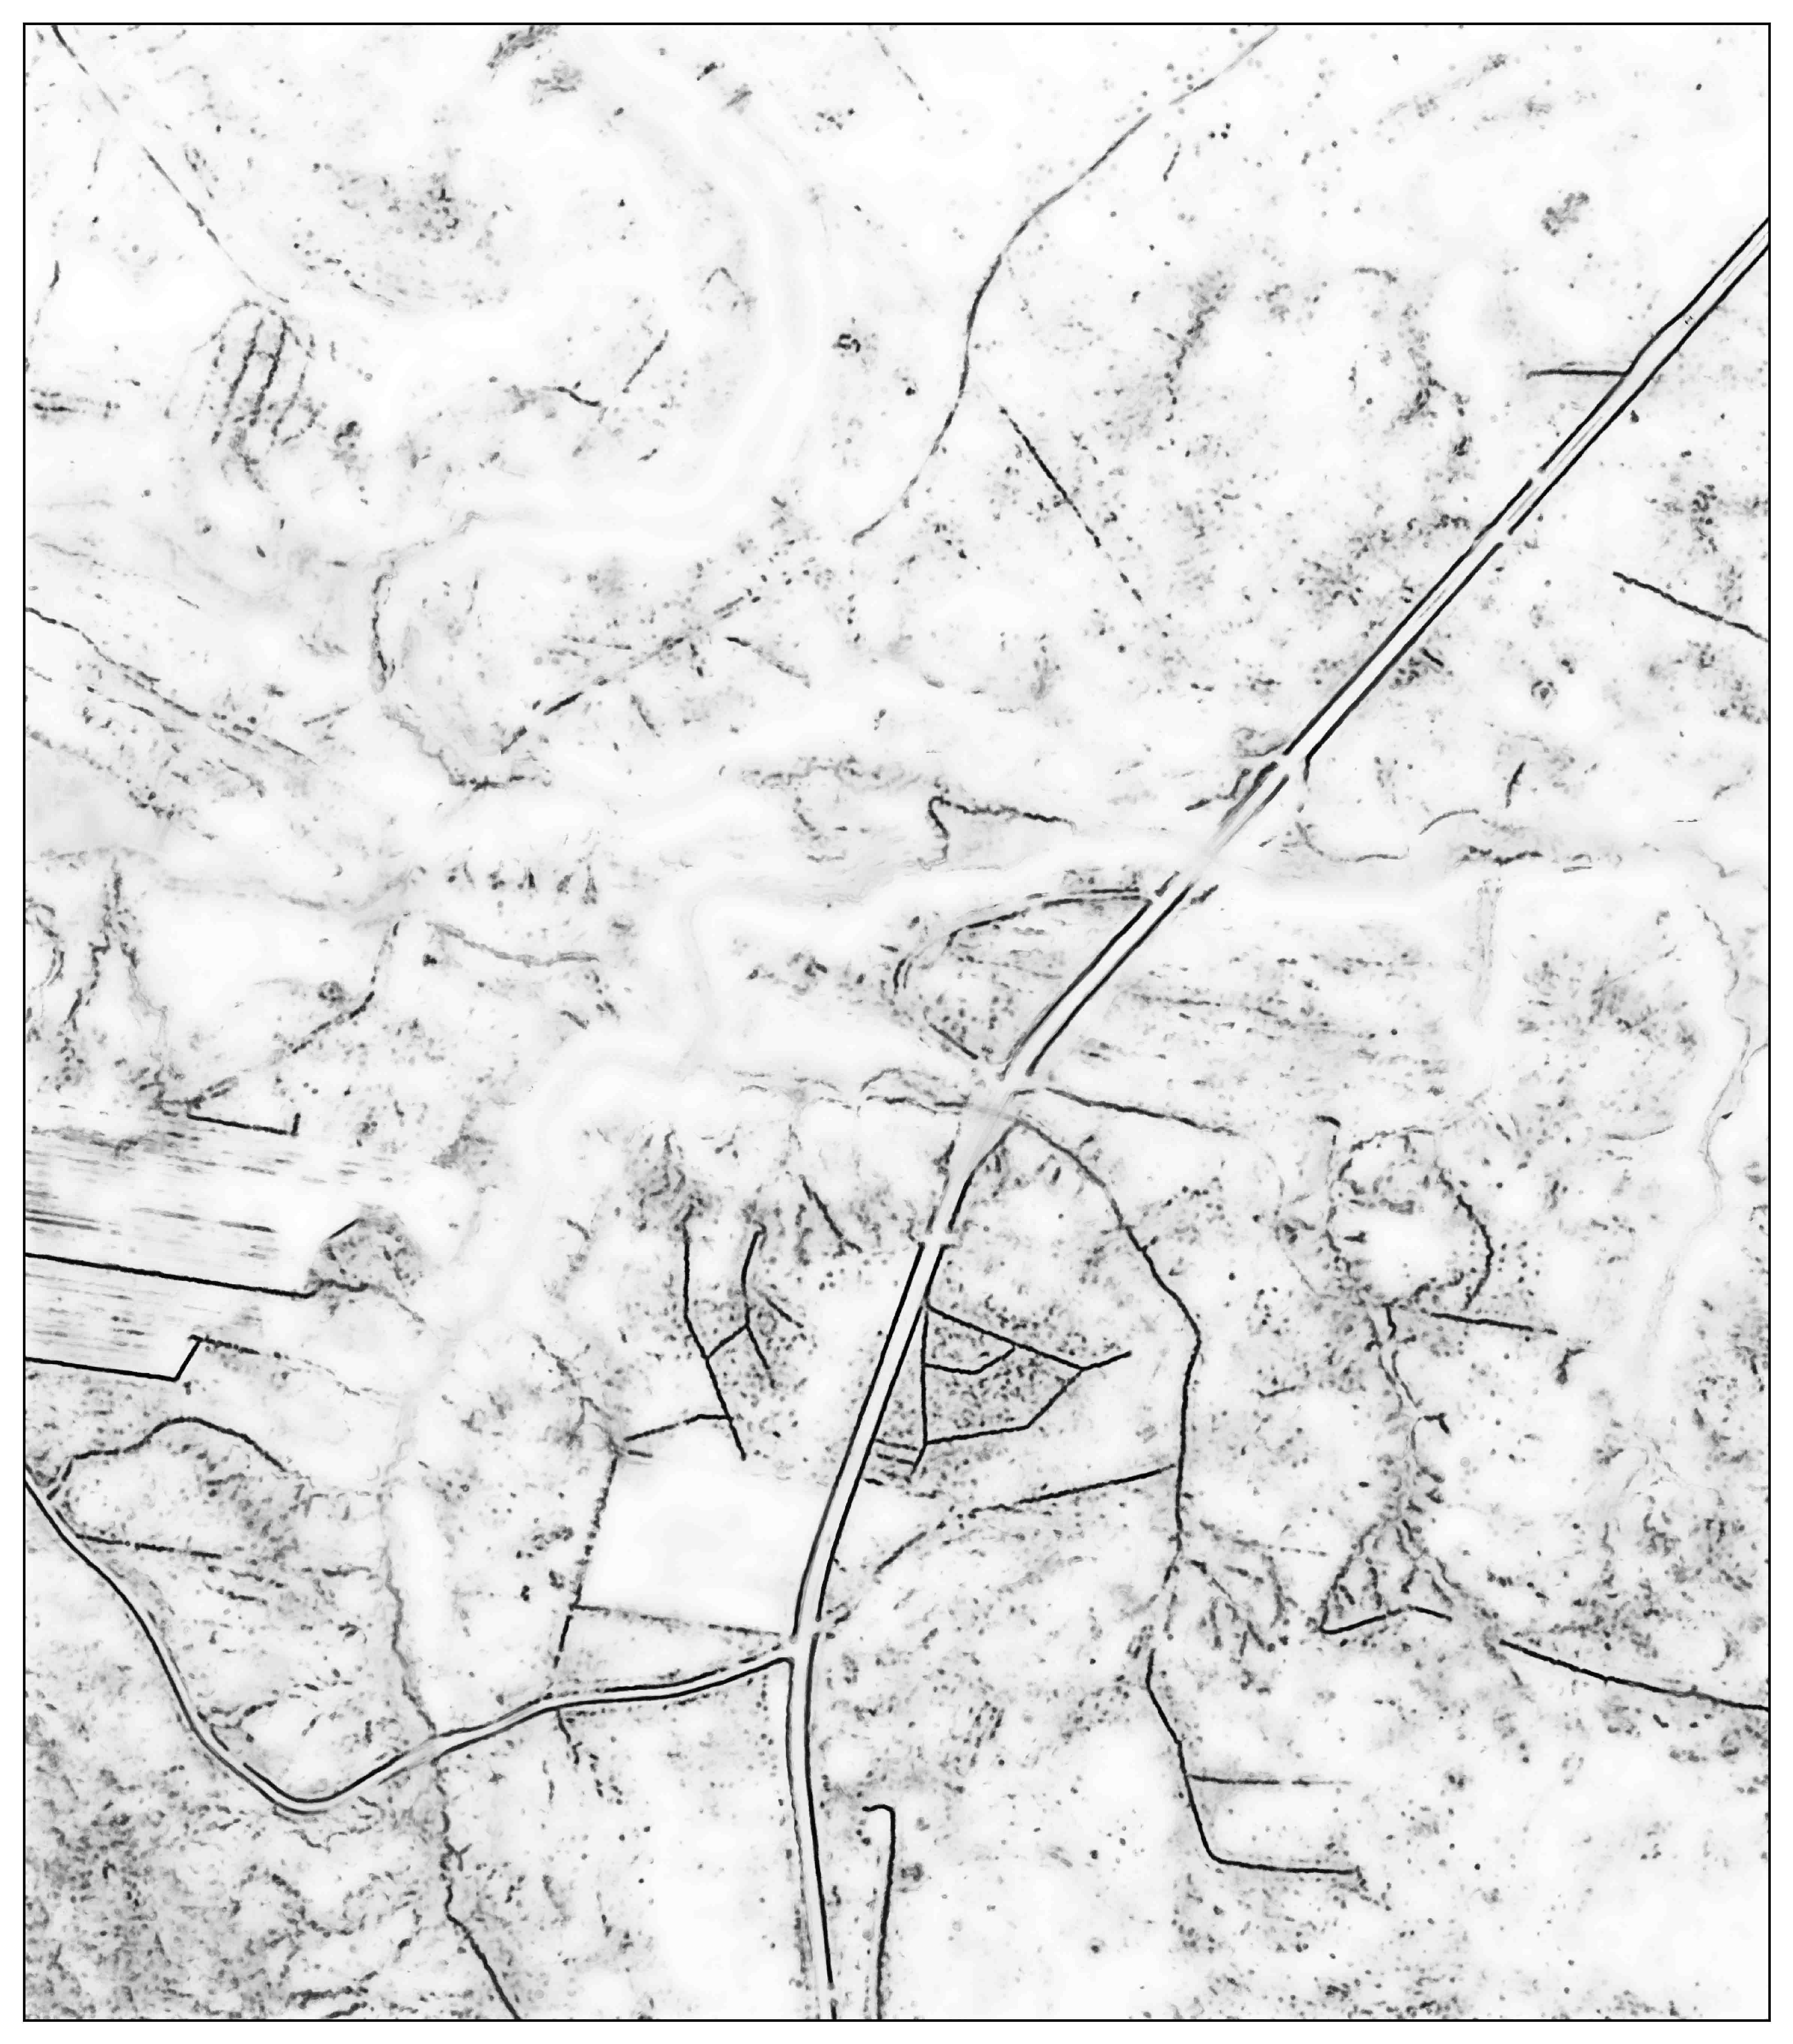
\includegraphics{./images/publ_post_process_step_2_lo.jpg}}}
    \DIFaddendFL \caption{\DIFdelbeginFL \DIFdelFL{Step one and two of the post-process. }\DIFdelendFL \DIFaddbeginFL \textbf{\DIFaddFL{Post-processing step one and two.}} \DIFaddendFL Darker pixels indicate a higher ditch probability. \textbf{a: }Random Forests probability prediction. \textbf{b: }Bilateral de-noising.}
    \label{fig:postprocessing1}
\end{figure}

\begin{figure} [!htb]
    \centering
    \DIFdelbeginFL %DIFDELCMD < \subfigure[]{
%DIFDELCMD <         \resizebox*{6.85cm}{!}{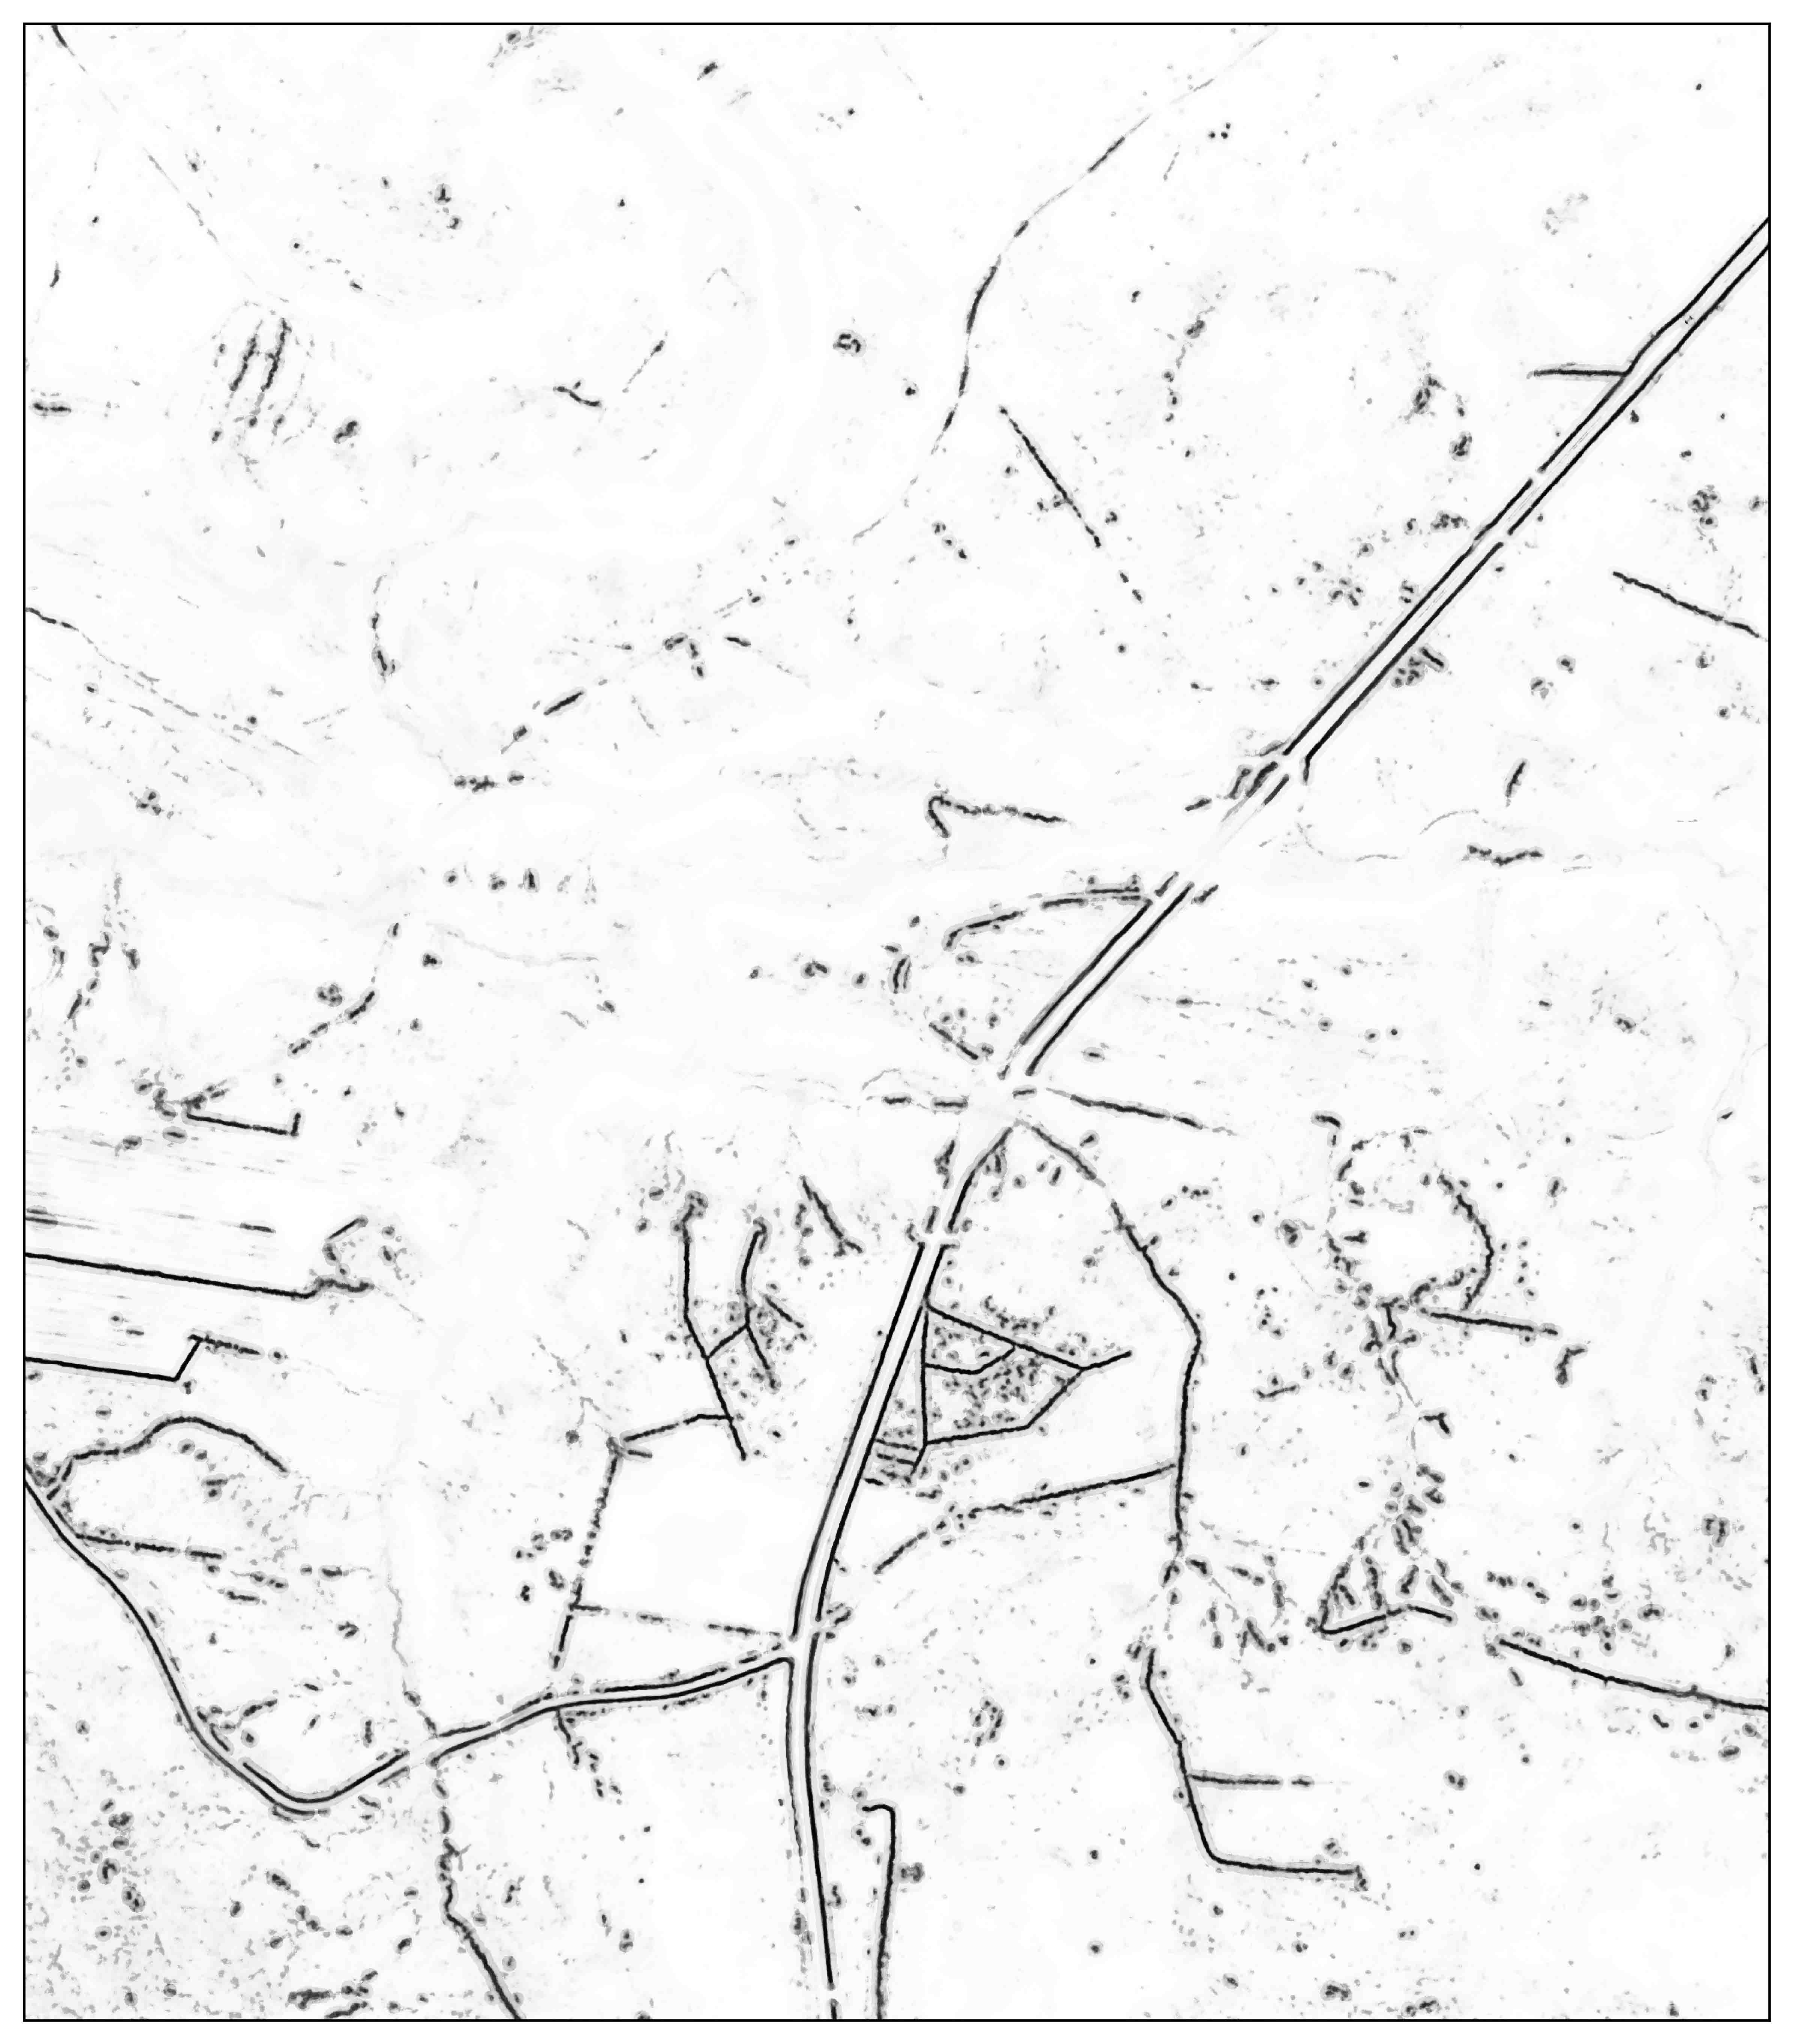
\includegraphics{./images/publ_post_process_step_3_lo.jpg}}}%%%
\DIFdelFL{\hspace{5pt}
    }%DIFDELCMD < \subfigure[]{
%DIFDELCMD <         \resizebox*{6.85cm}{!}{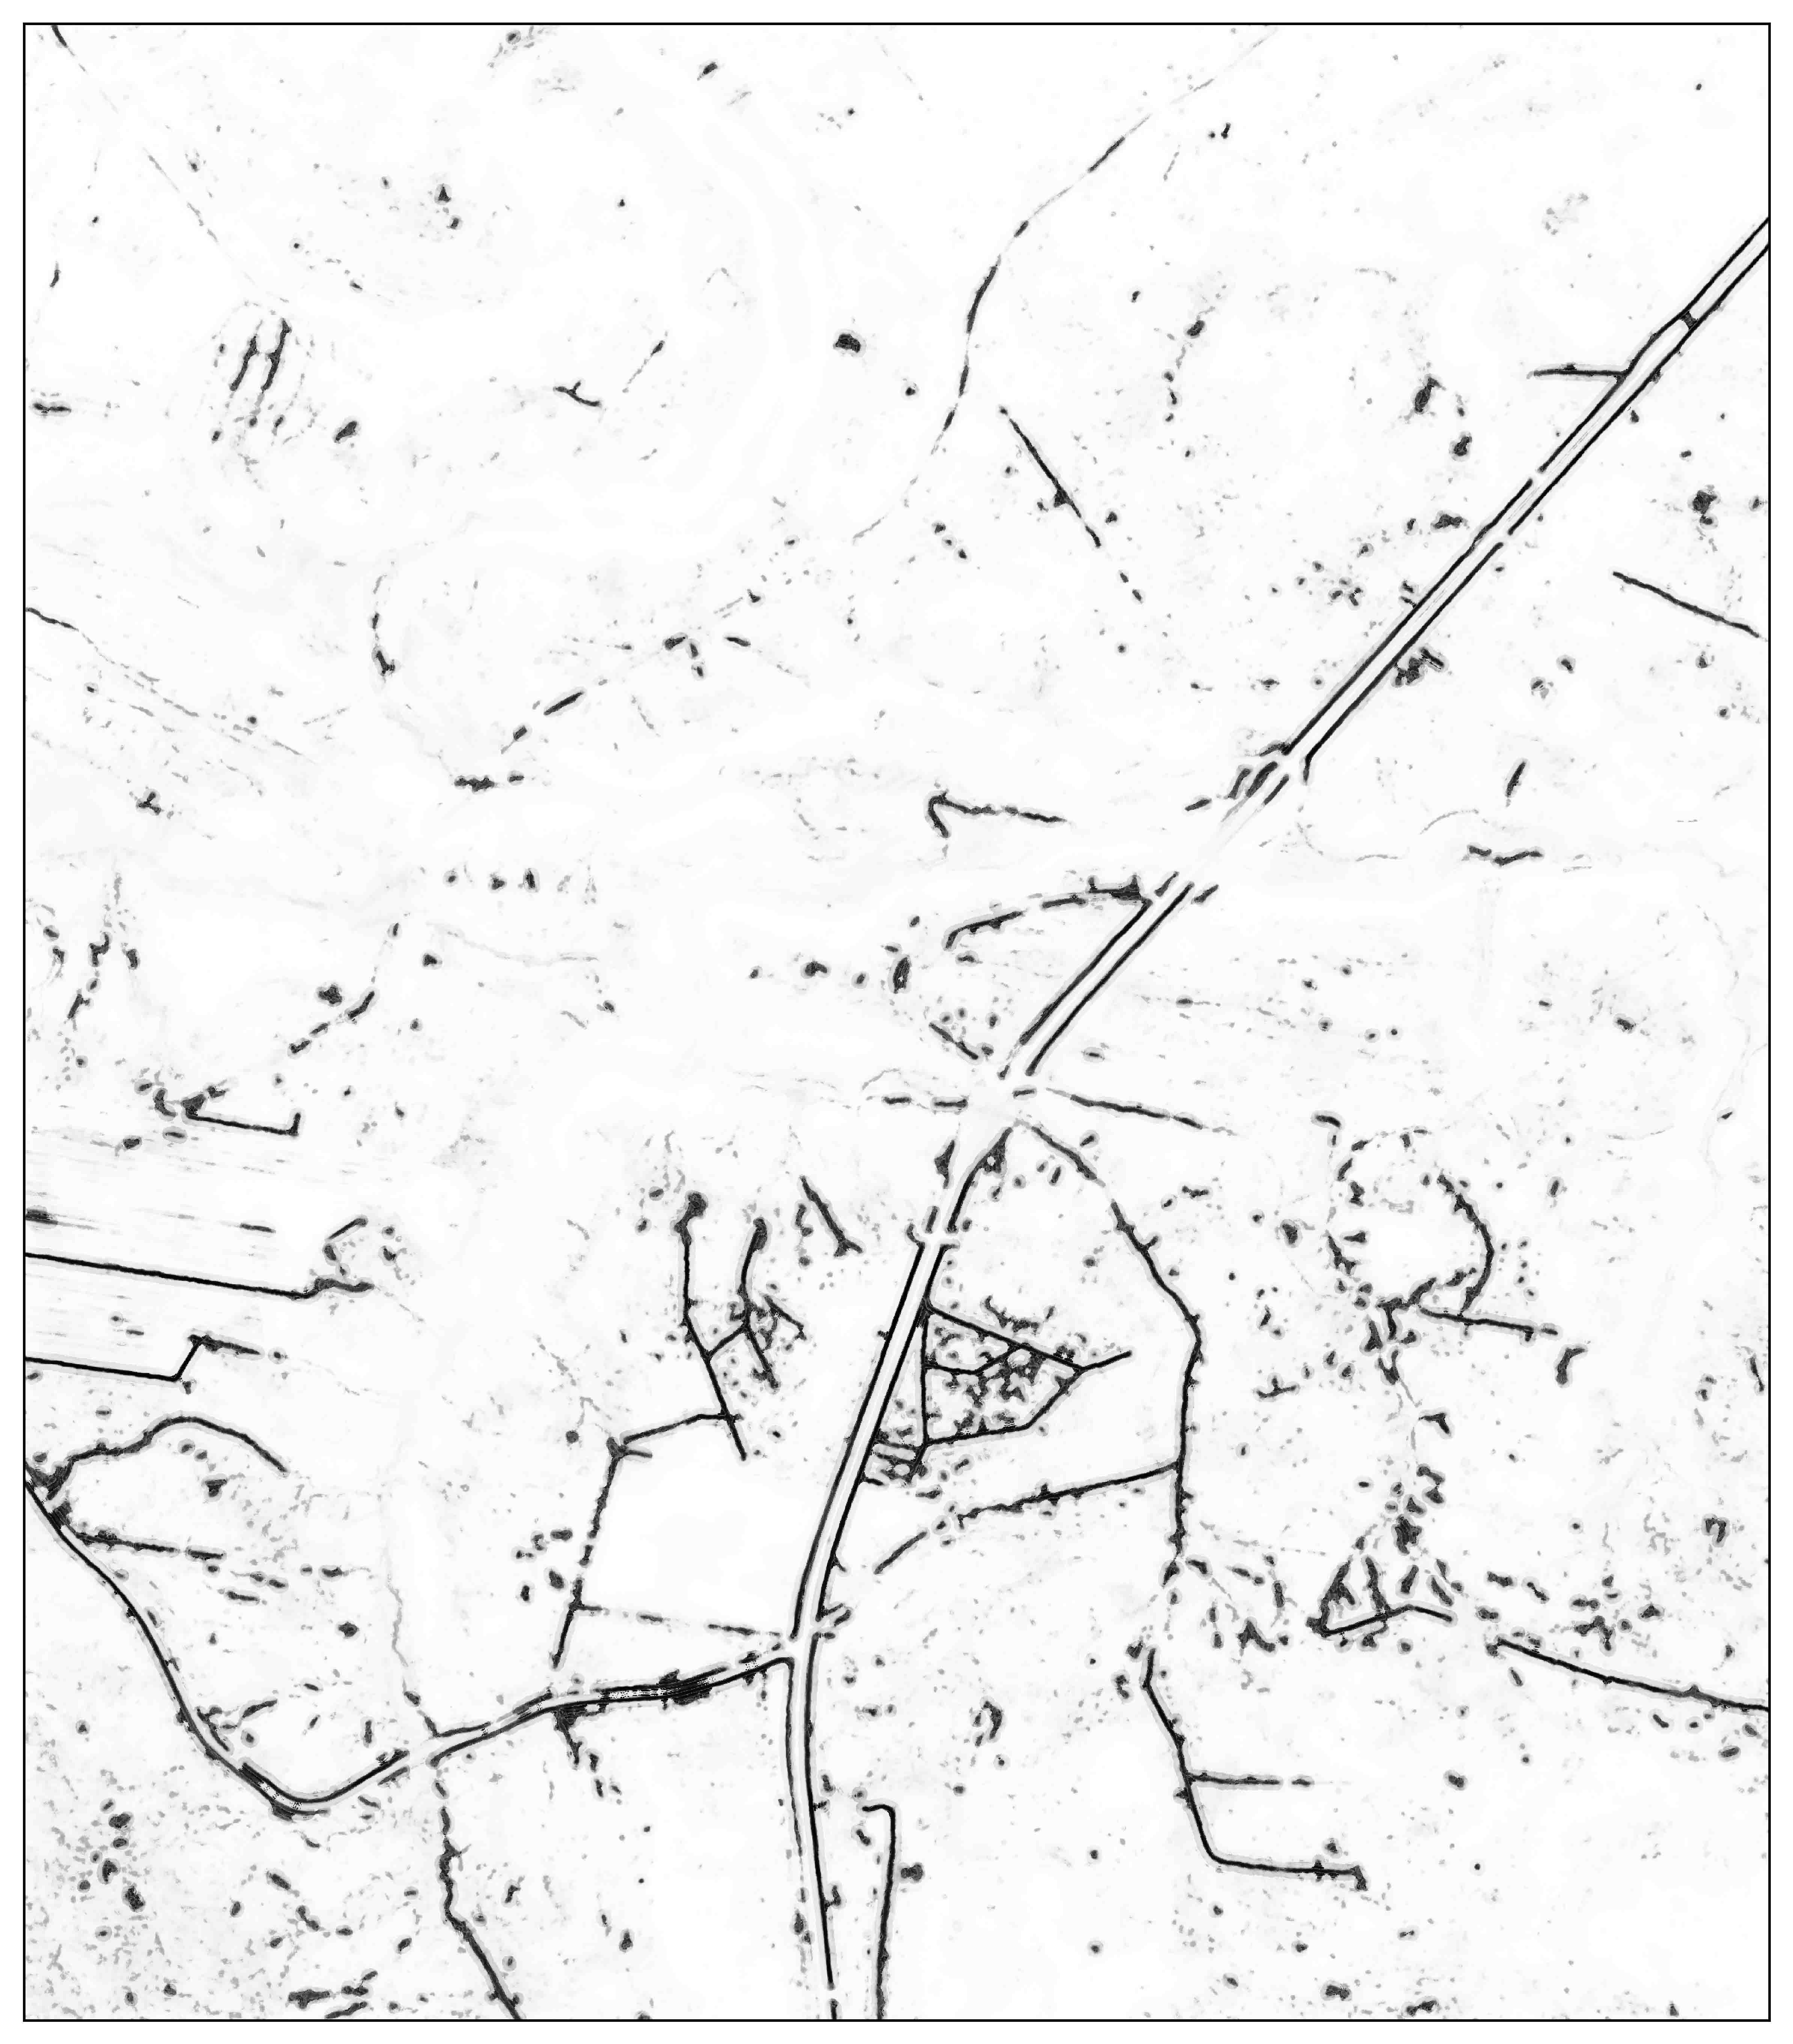
\includegraphics{./images/publ_post_process_step_4_lo.jpg}}}
%DIFDELCMD <     %%%
\DIFdelendFL \DIFaddbeginFL \subfigure[]{
        \resizebox*{5.6cm}{!}{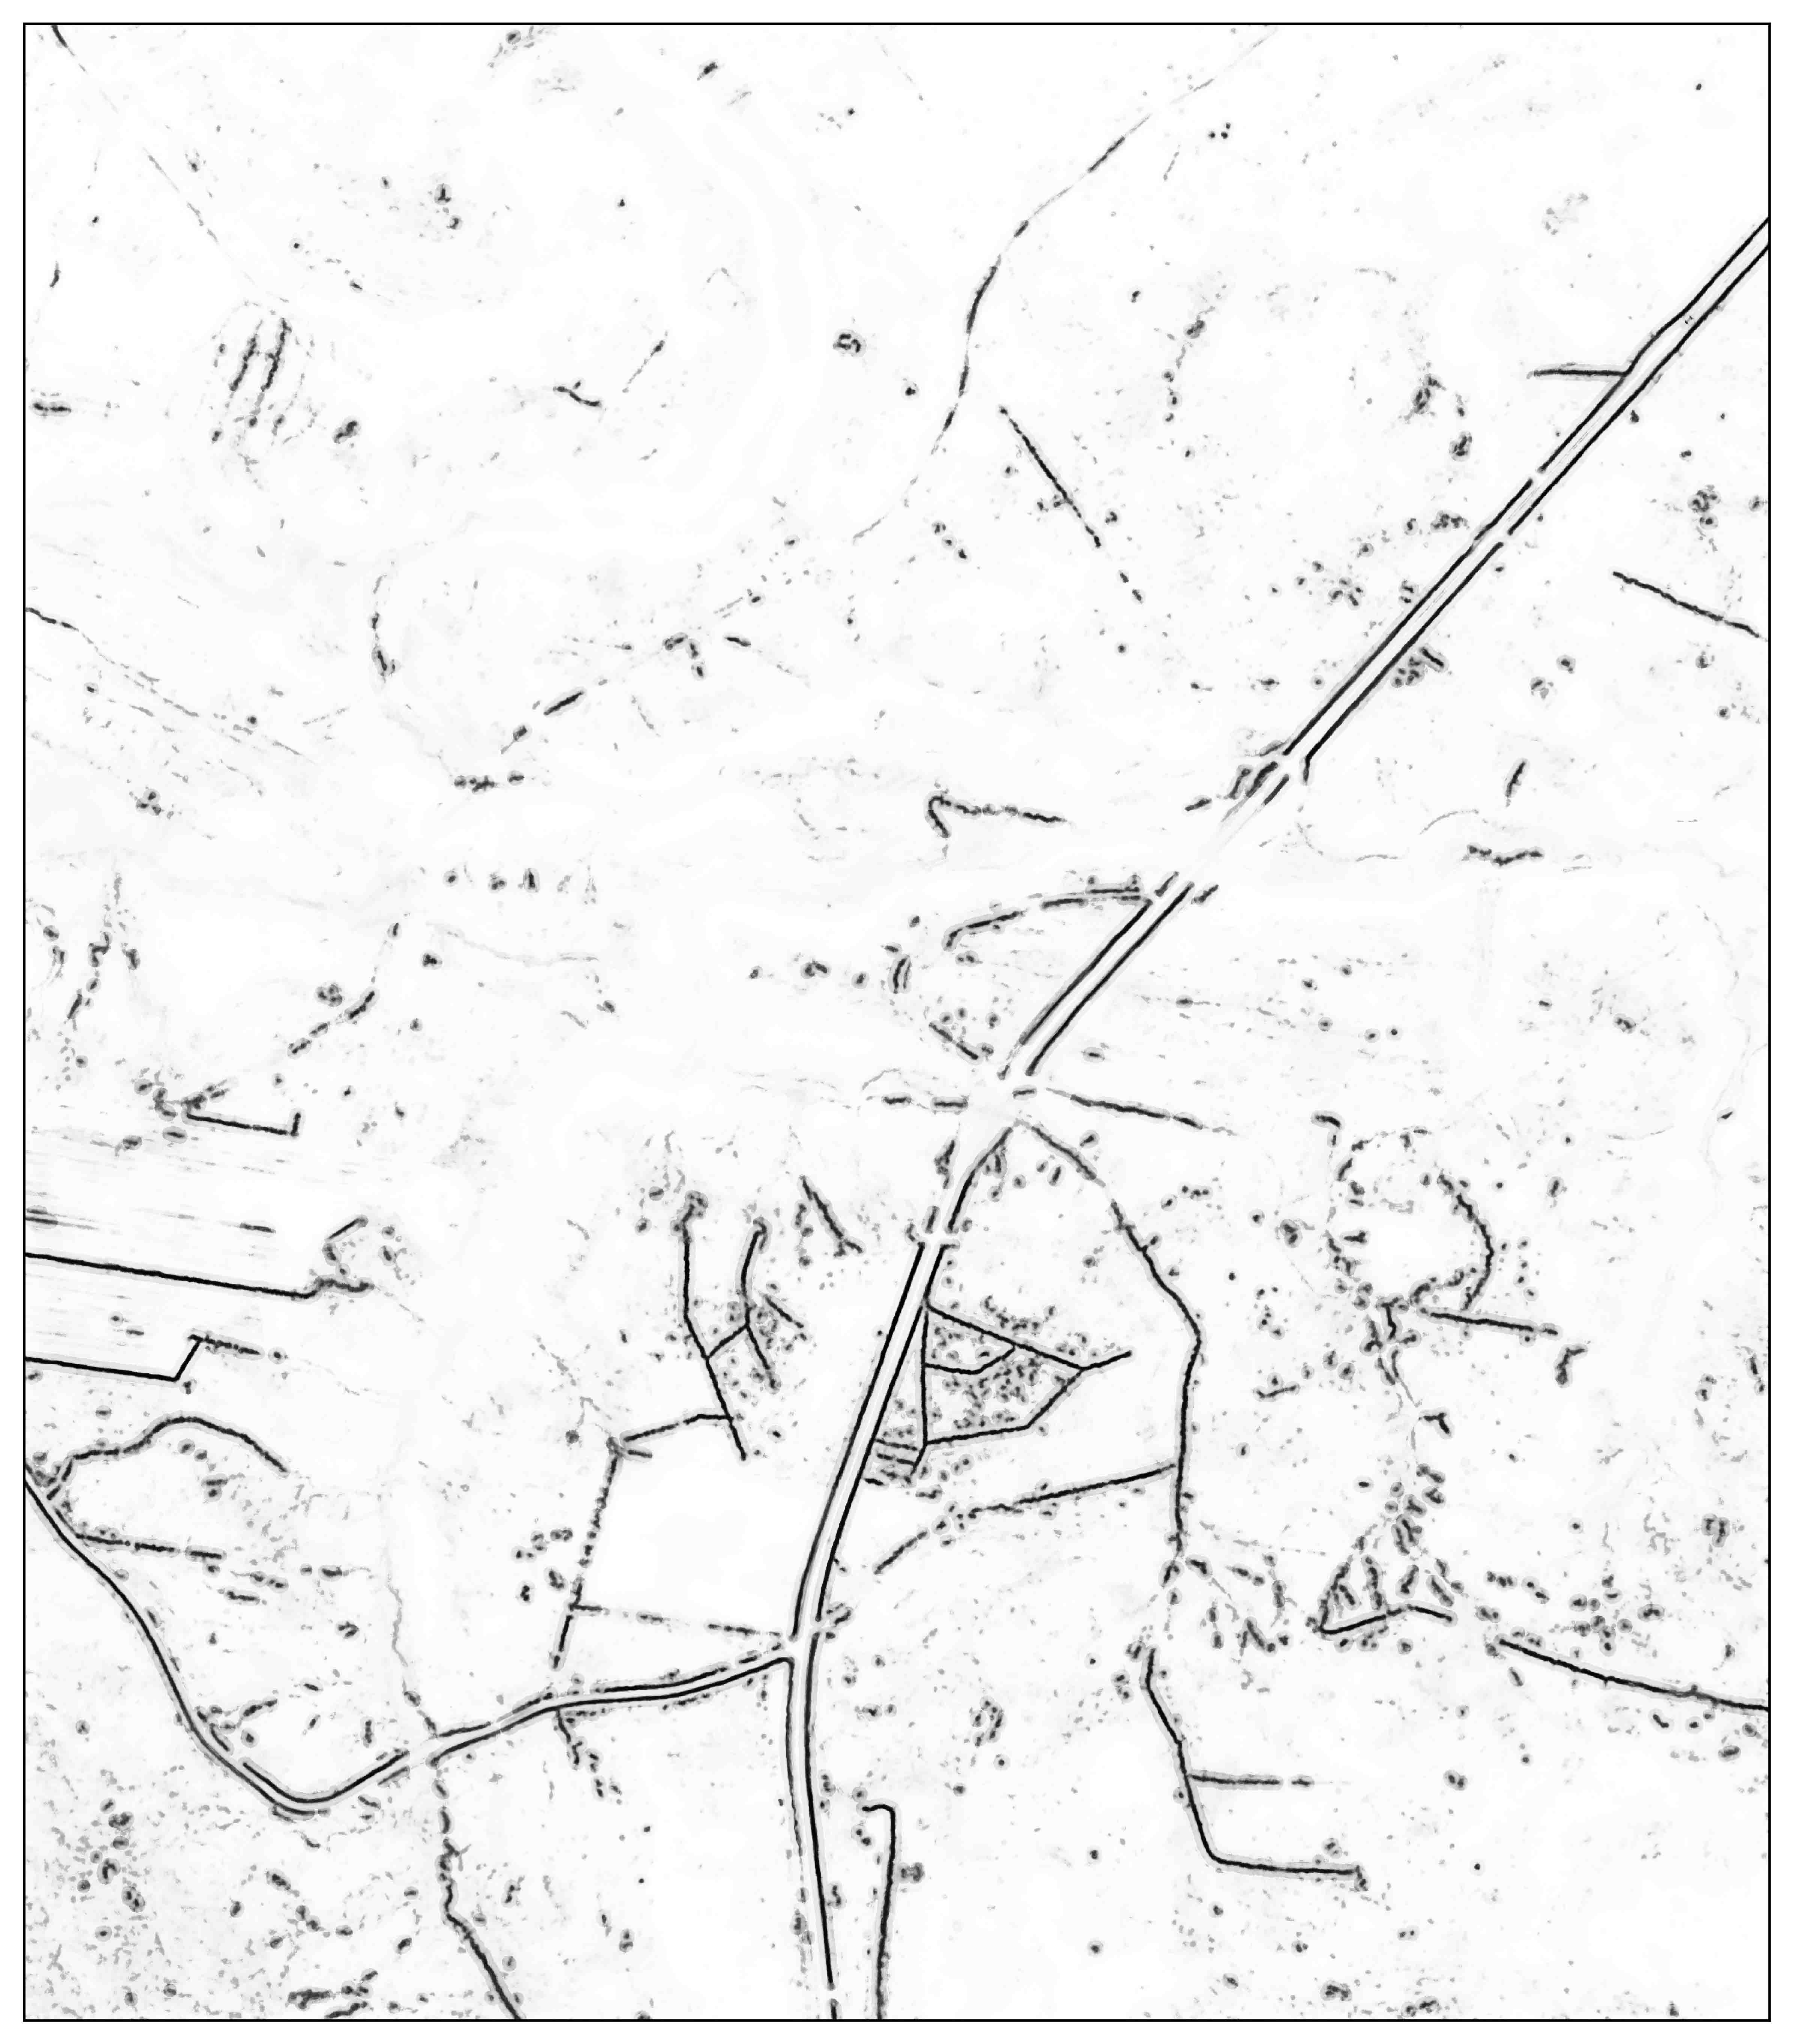
\includegraphics{./images/publ_post_process_step_3_lo.jpg}}}\DIFaddFL{\hspace{5pt}
    }\subfigure[]{
        \resizebox*{5.6cm}{!}{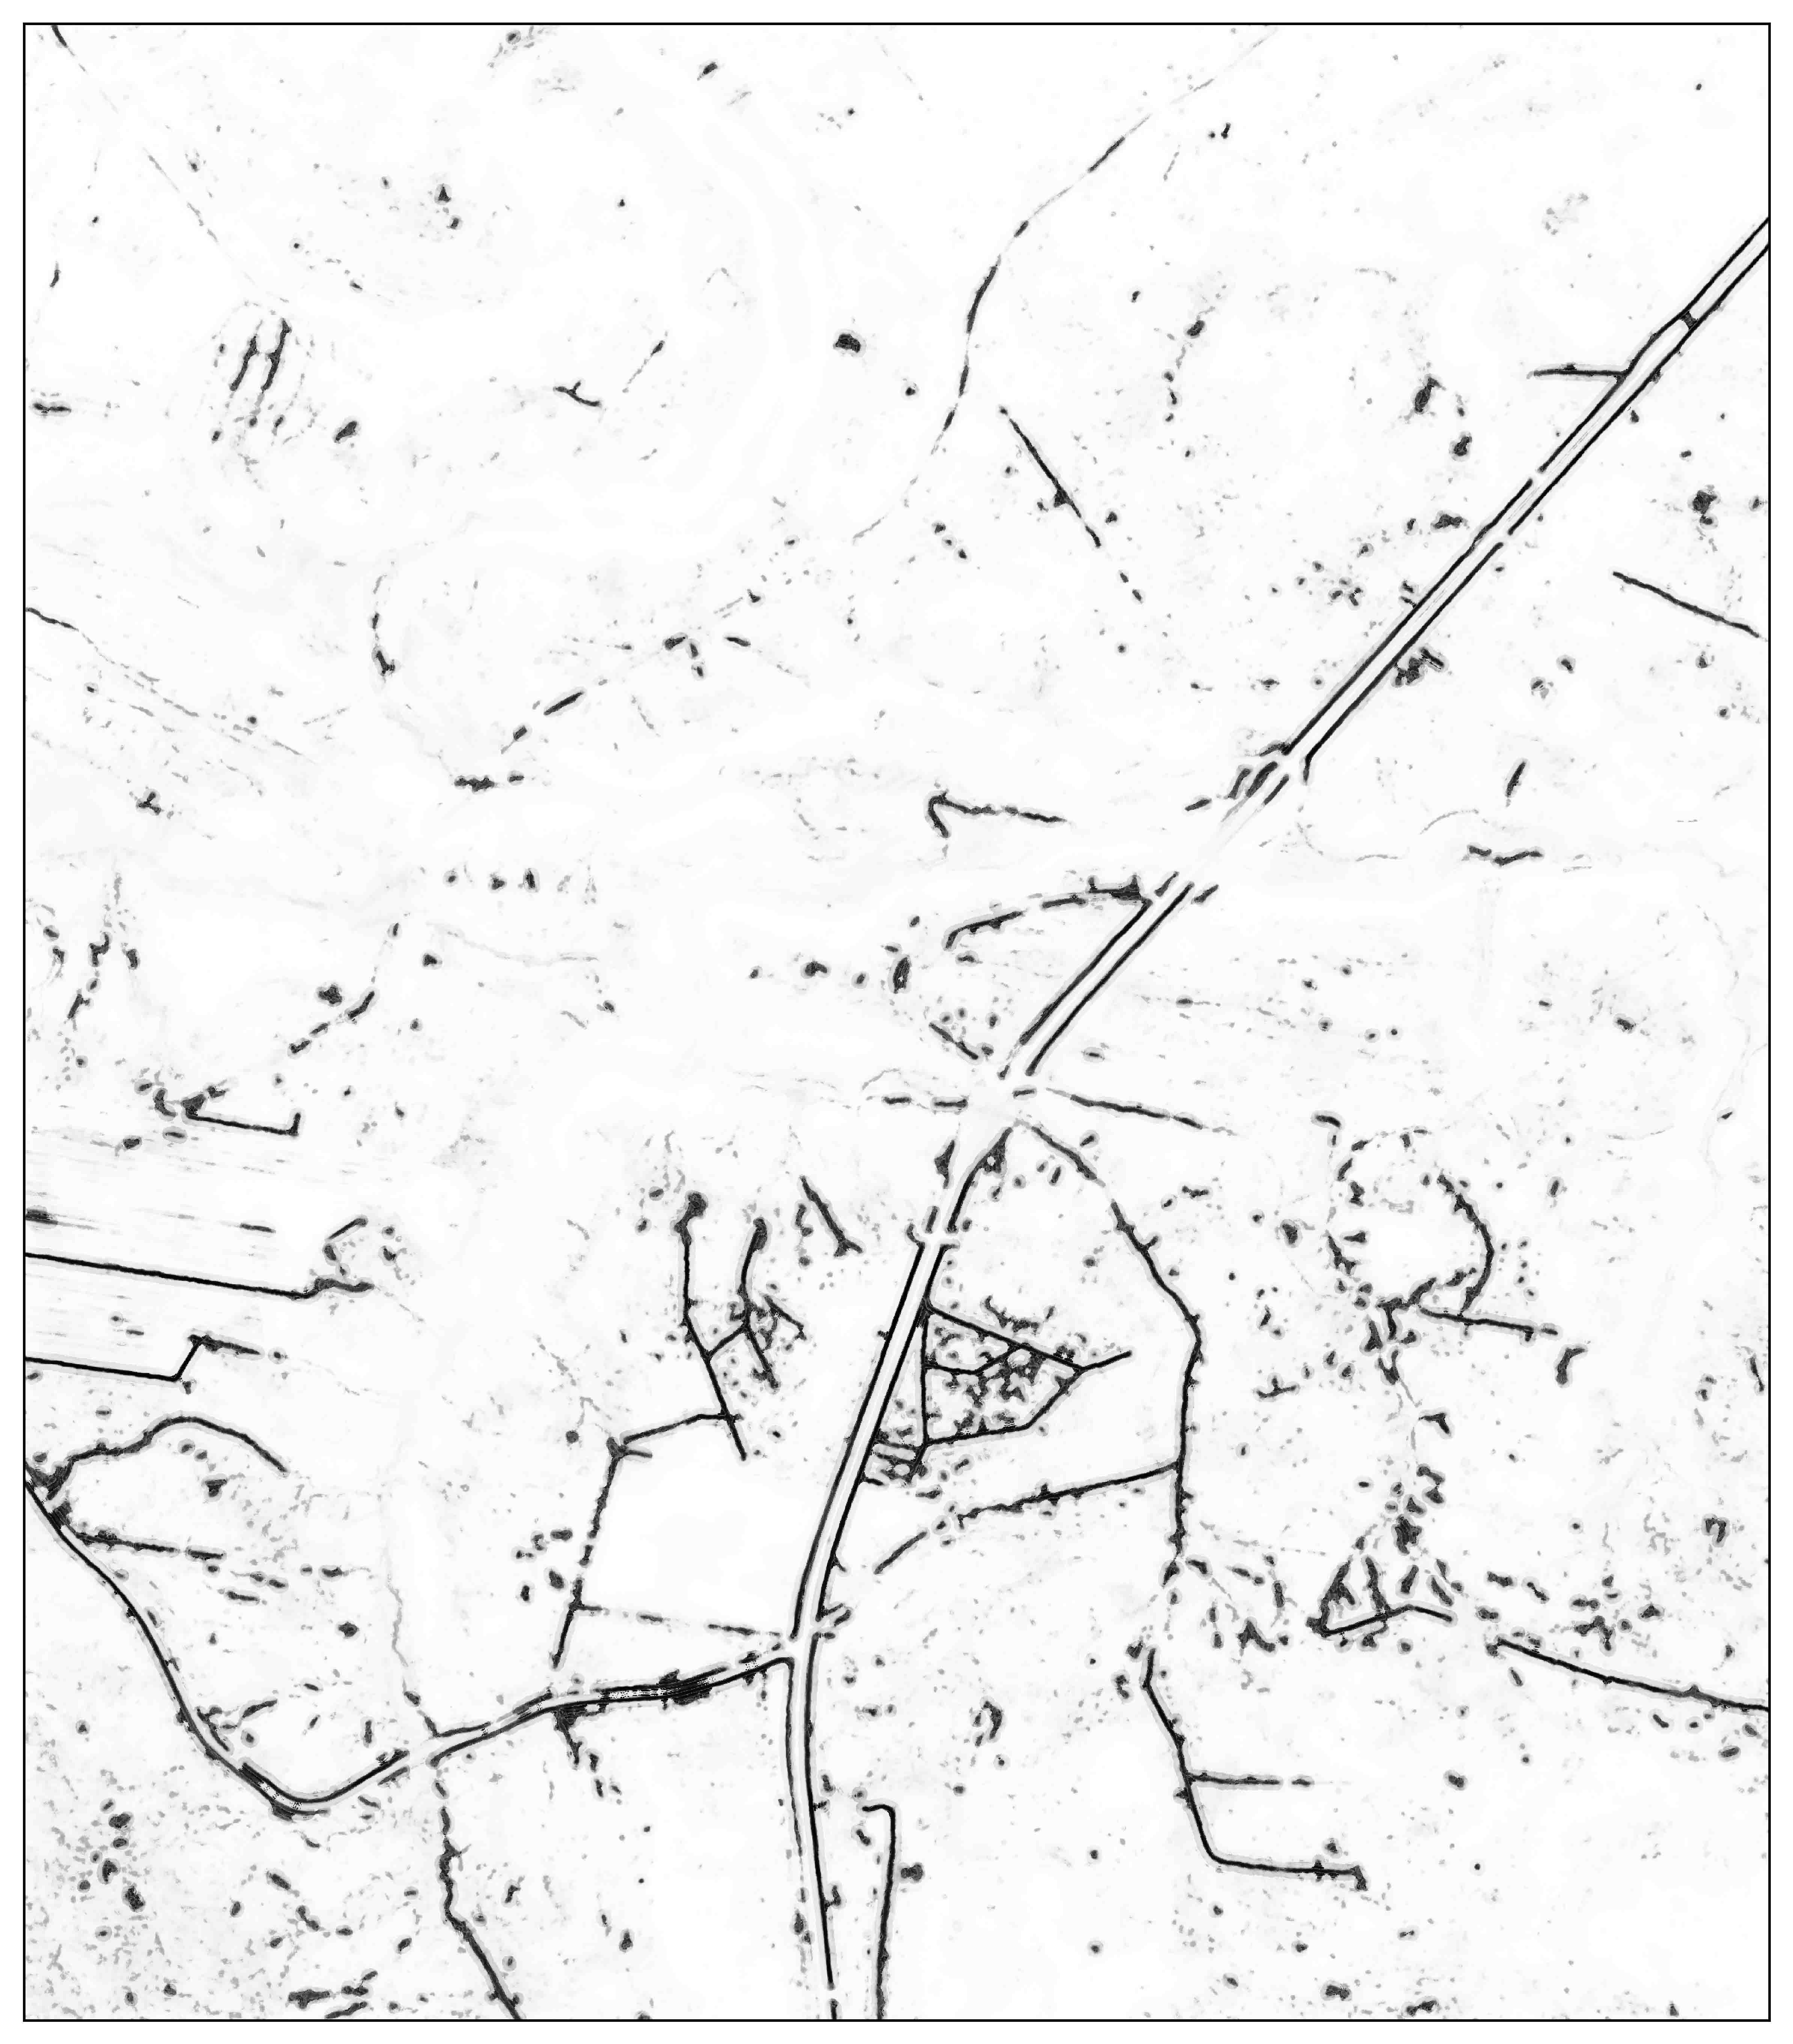
\includegraphics{./images/publ_post_process_step_4_lo.jpg}}}
    \DIFaddendFL \caption{\DIFdelbeginFL \DIFdelFL{Step three and four of the post-process. }\DIFdelendFL \DIFaddbeginFL \textbf{\DIFaddFL{Post-processing step three and four.}} \DIFaddendFL Darker pixels indicate a higher ditch probability. \textbf{a: }Custom de-noising. \textbf{b: }Gap filling.}
    \label{fig:postprocessing2}
\end{figure}

\subsubsection{Binarisation \DIFdelbegin \DIFdel{with grid zones}\DIFdelend \DIFaddbegin \DIFadd{and cluster removal}\DIFaddend }
\DIFdelbegin \DIFdel{The models' ditch prediction is given in the original resolution raster format. To allow for comparison to the evaluation data, the same grid conversion was performed on the prediction raster as on the evaluation data displayed in }%DIFDELCMD < \hyperref[fig:ditchpreprocess]{Figure} %%%
\DIFdel{\ref{fig:ditchpreprocess} }%DIFDELCMD < \hyperref[fig:ditchpreprocess]{c}%%%
\DIFdel{. After testing different combinations of zone sizes and probability values, a mean probability rating was calculated for }\DIFdelend \DIFaddbegin 

\DIFadd{To correct errors where lone pixels inside ditches had been incorrectly classified, the resolution was lowered by binary classifying }\DIFaddend each $6*6$ \DIFdelbegin \DIFdel{grid zone, classifying the entire zone as part of a ditch }\DIFdelend \DIFaddbegin \DIFadd{pixel grid as a ditch or a non-ditch }\DIFaddend if the mean probability \DIFaddbegin \DIFadd{of the pixels inside the grid }\DIFaddend exceeded 40 \% \DIFdelbegin \DIFdel{. This zone partitioning helped to fill in gaps where lone pixels in ditches had been incorrectly classified. }\DIFdelend (\hyperref[fig:postprocessing3]{Figure} \ref{fig:postprocessing3} \hyperref[fig:postprocessing3]{a}). \DIFaddbegin \DIFadd{The same zone partitioning was performed on the labels (}\hyperref[fig:ditchpreprocess]{Figure} \DIFadd{\ref{fig:ditchpreprocess} }\hyperref[fig:ditchpreprocess]{c}\DIFadd{).
}\DIFaddend 

\DIFdelbegin \subsubsection{\DIFdel{Cluster removal}}
%DIFAUXCMD
\addtocounter{subsubsection}{-1}%DIFAUXCMD
\DIFdel{To }\DIFdelend \DIFaddbegin \DIFadd{A cluster detection algorithm was developed to }\DIFaddend remove noise from the \DIFdelbegin \DIFdel{binary prediction, a custom cluster detection algorithm was used}\DIFdelend \DIFaddbegin \DIFadd{final ditch prediction}\DIFaddend . By finding the number of connected pixels with a true value and removing those whose cluster size were below a \DIFdelbegin \DIFdel{given }\DIFdelend threshold, minor noise in the prediction could be removed while still retaining most of the ditch pixels. \DIFdelbegin \DIFdel{Actual ditches that have a low probability and therefore create small clusters may still be excluded by this method, but the noise removal advantages were judged to outweigh the loss in recall. }\DIFdelend A distance calculation was also performed in tandem with this method to find the largest distance of pixels inside each given cluster. This helped to remove sinks and hollows that were not removed by the initial small cluster removal, but that did not have a linear directional characteristic, indicating that they did not represent a ditch (\hyperref[fig:postprocessing3]{Figure} \ref{fig:postprocessing3} \hyperref[fig:postprocessing3]{b}).

\begin{figure} [!htb]
    \centering
    \DIFdelbeginFL %DIFDELCMD < \subfigure[]{
%DIFDELCMD <         \resizebox*{6.85cm}{!}{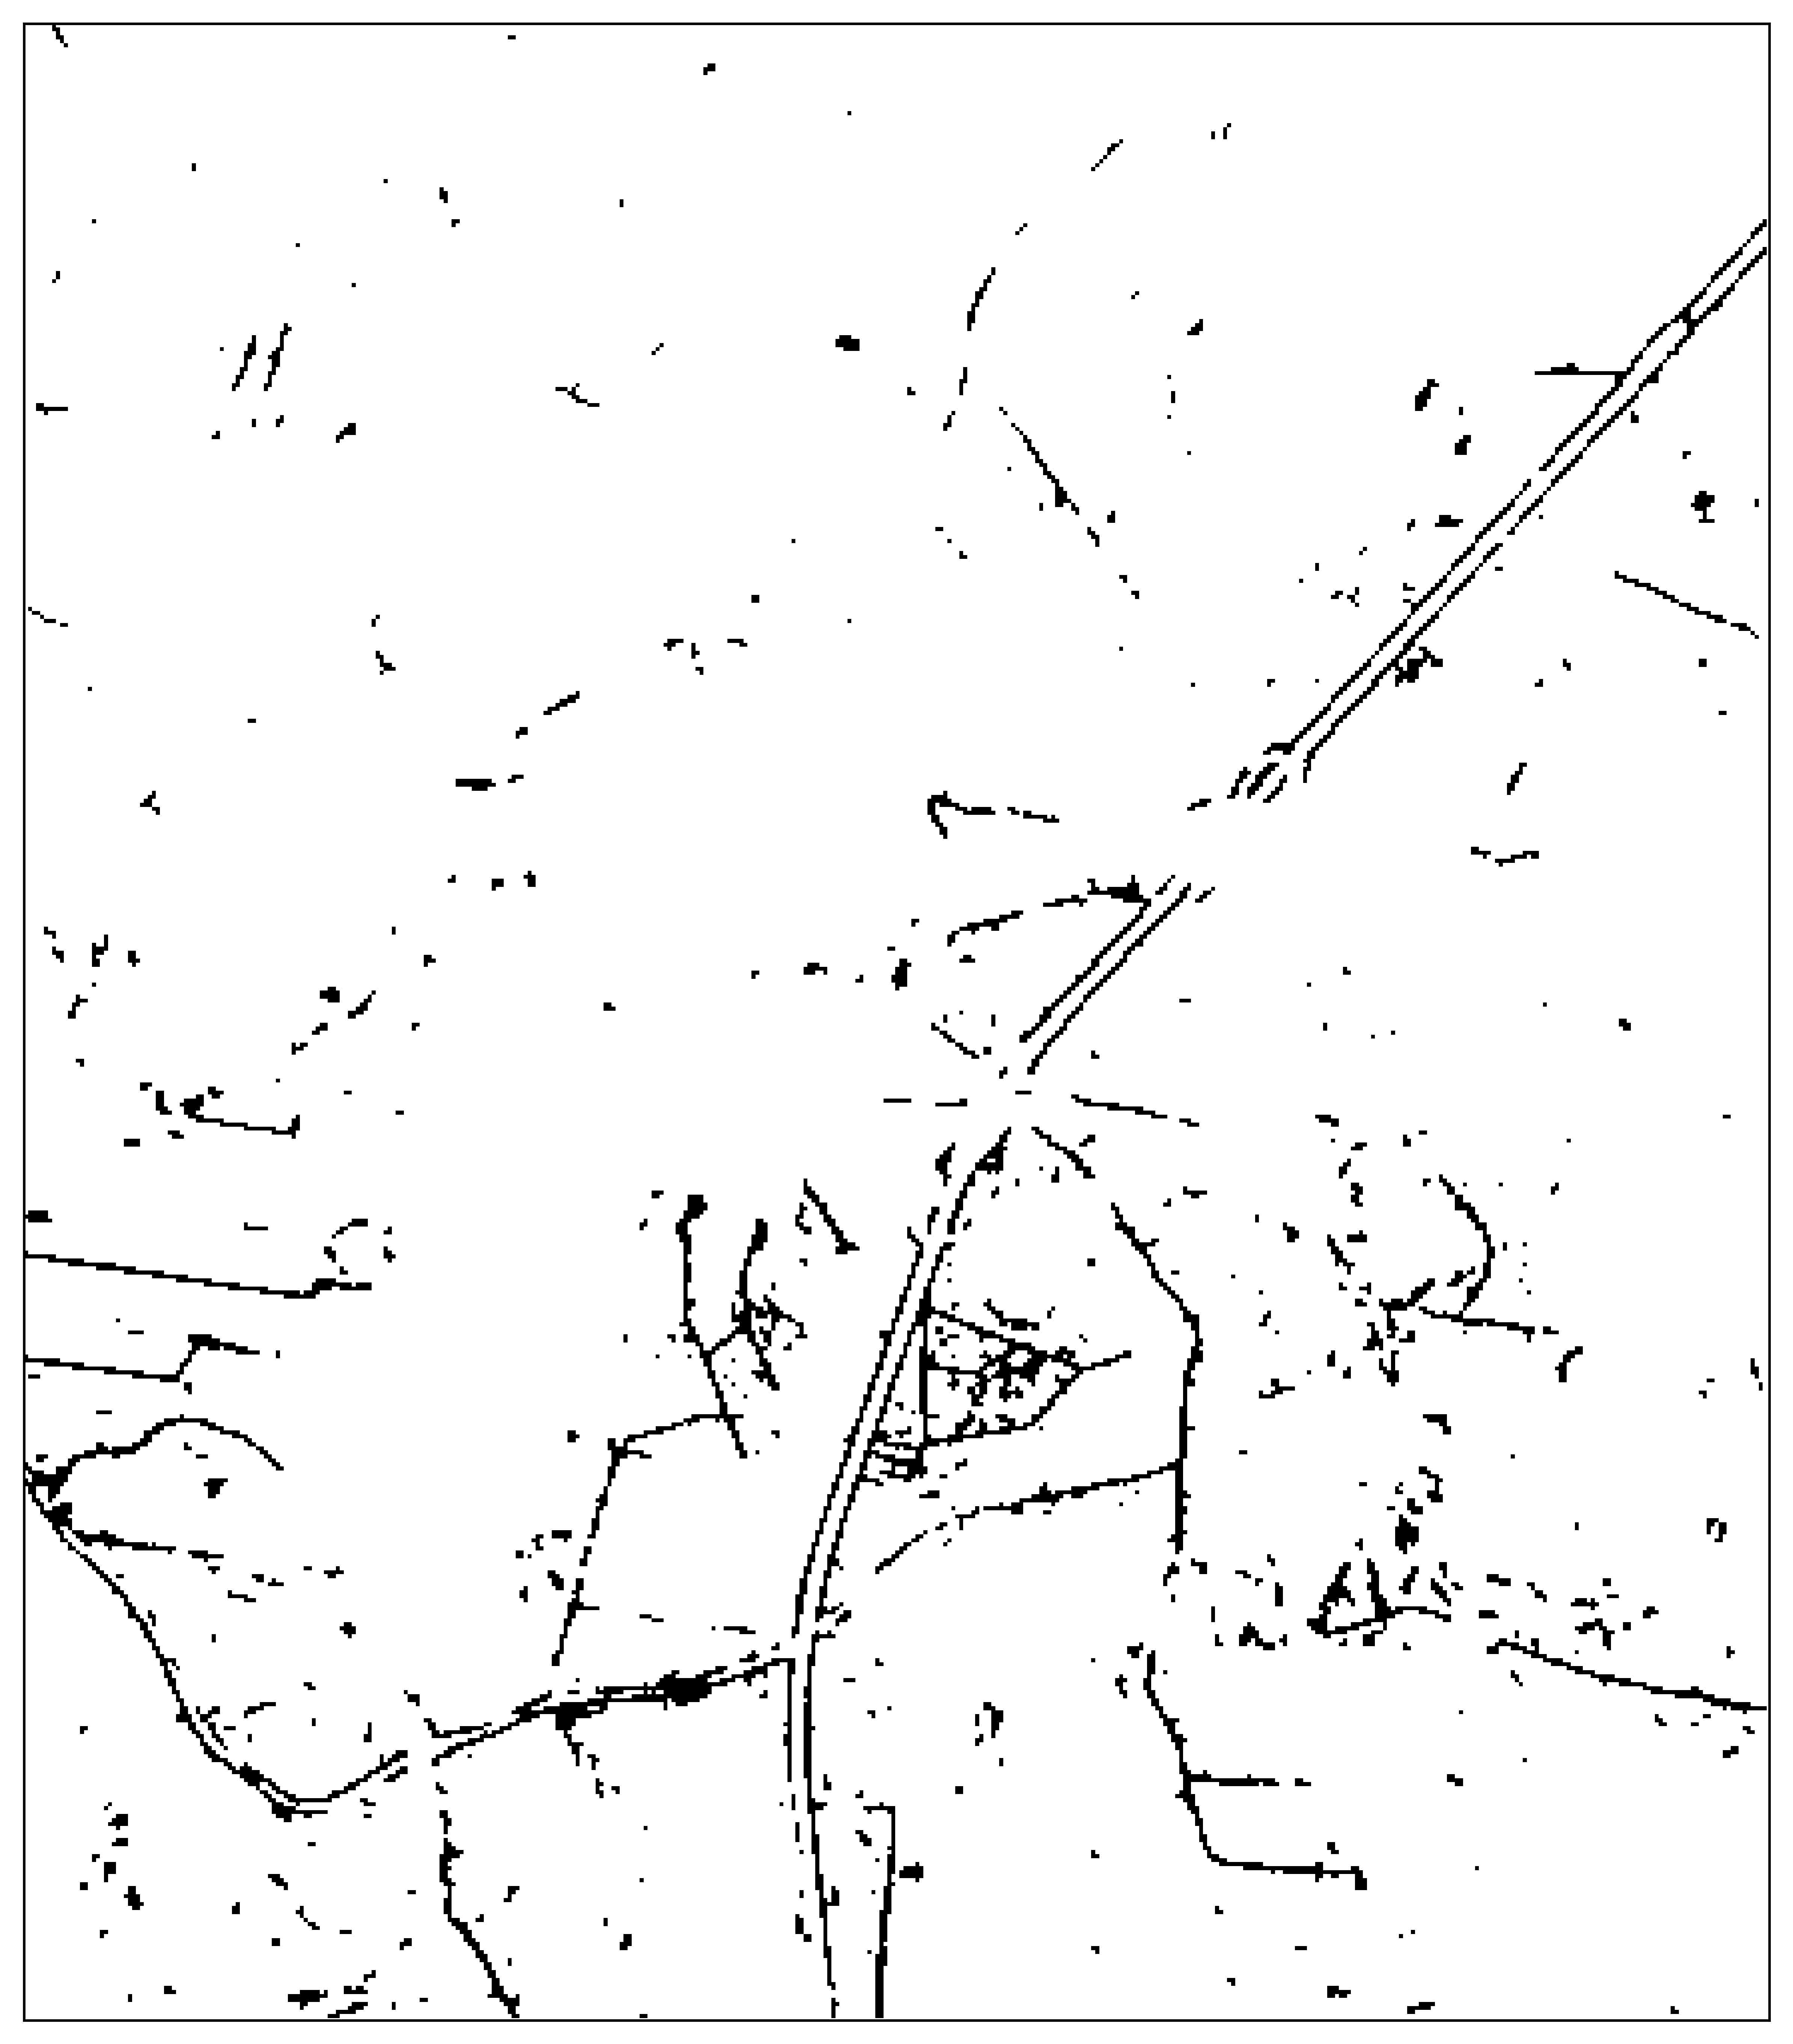
\includegraphics{./images/publ_post_process_step_5_lo.jpg}}}%%%
\DIFdelFL{\hspace{5pt}
    }%DIFDELCMD < \subfigure[]{
%DIFDELCMD <         \resizebox*{6.85cm}{!}{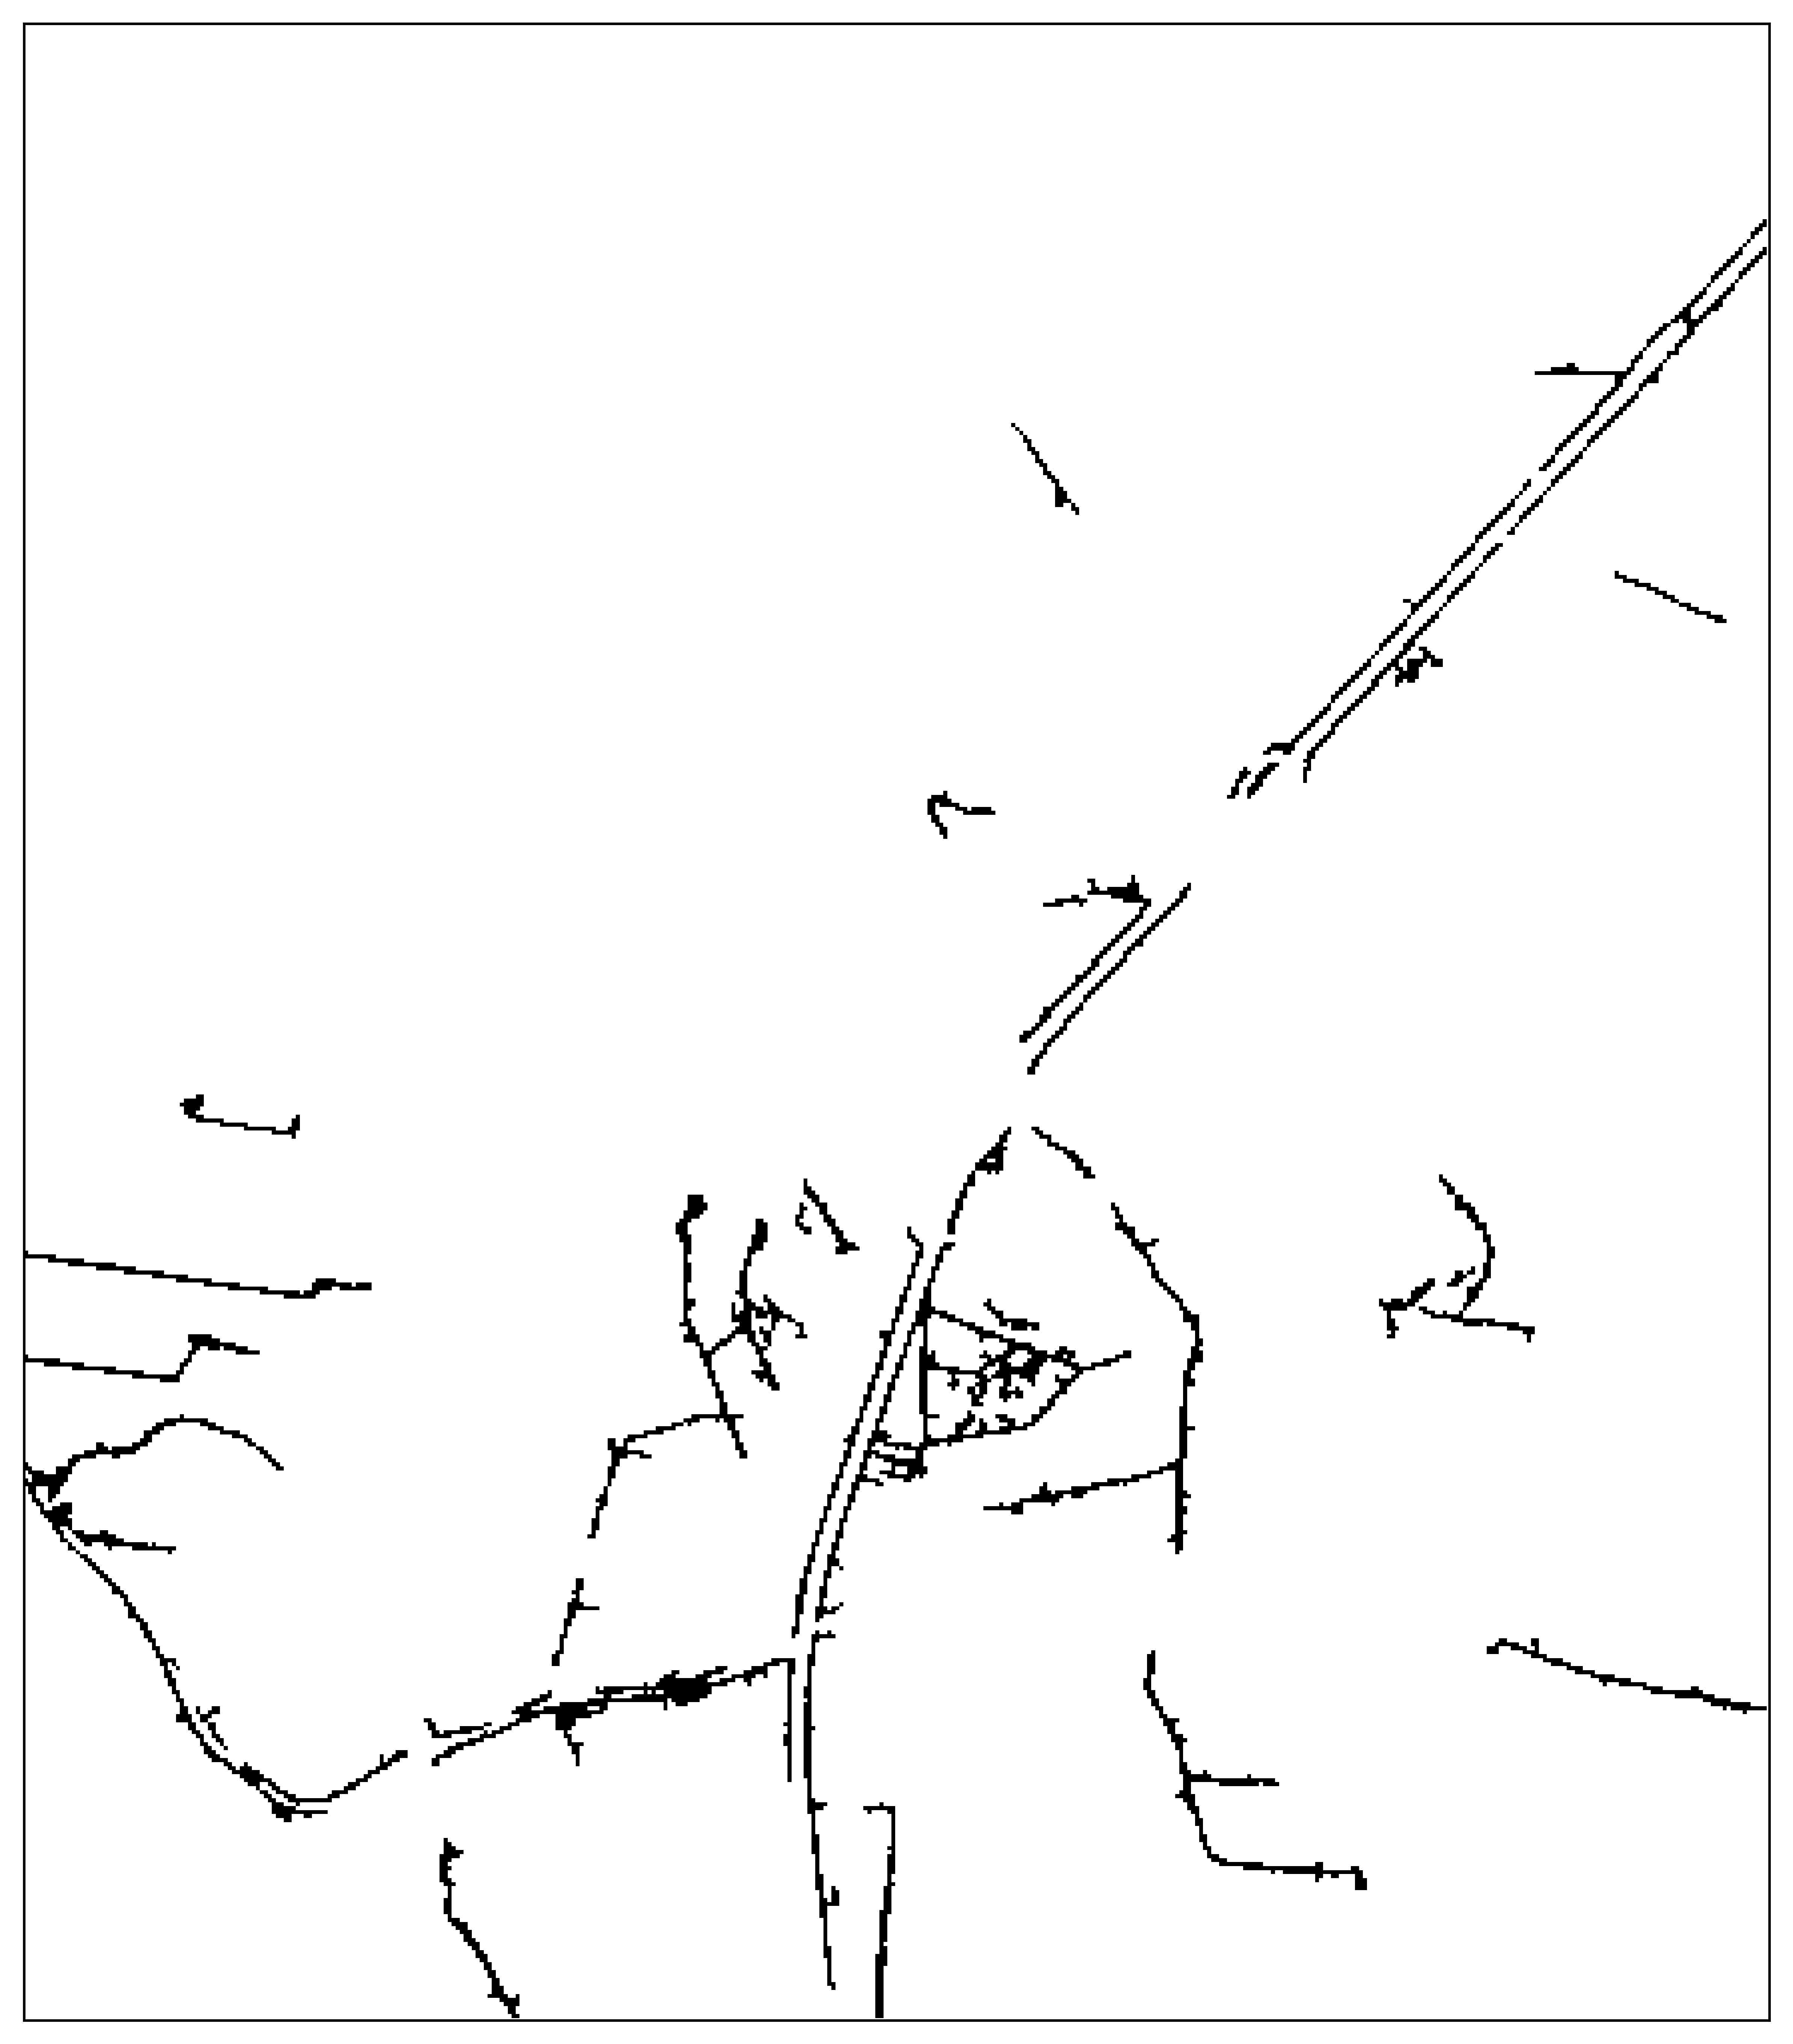
\includegraphics{./images/publ_post_process_step_6_lo.jpg}}}
%DIFDELCMD <     %%%
\DIFdelendFL \DIFaddbeginFL \subfigure[]{
        \resizebox*{5.6cm}{!}{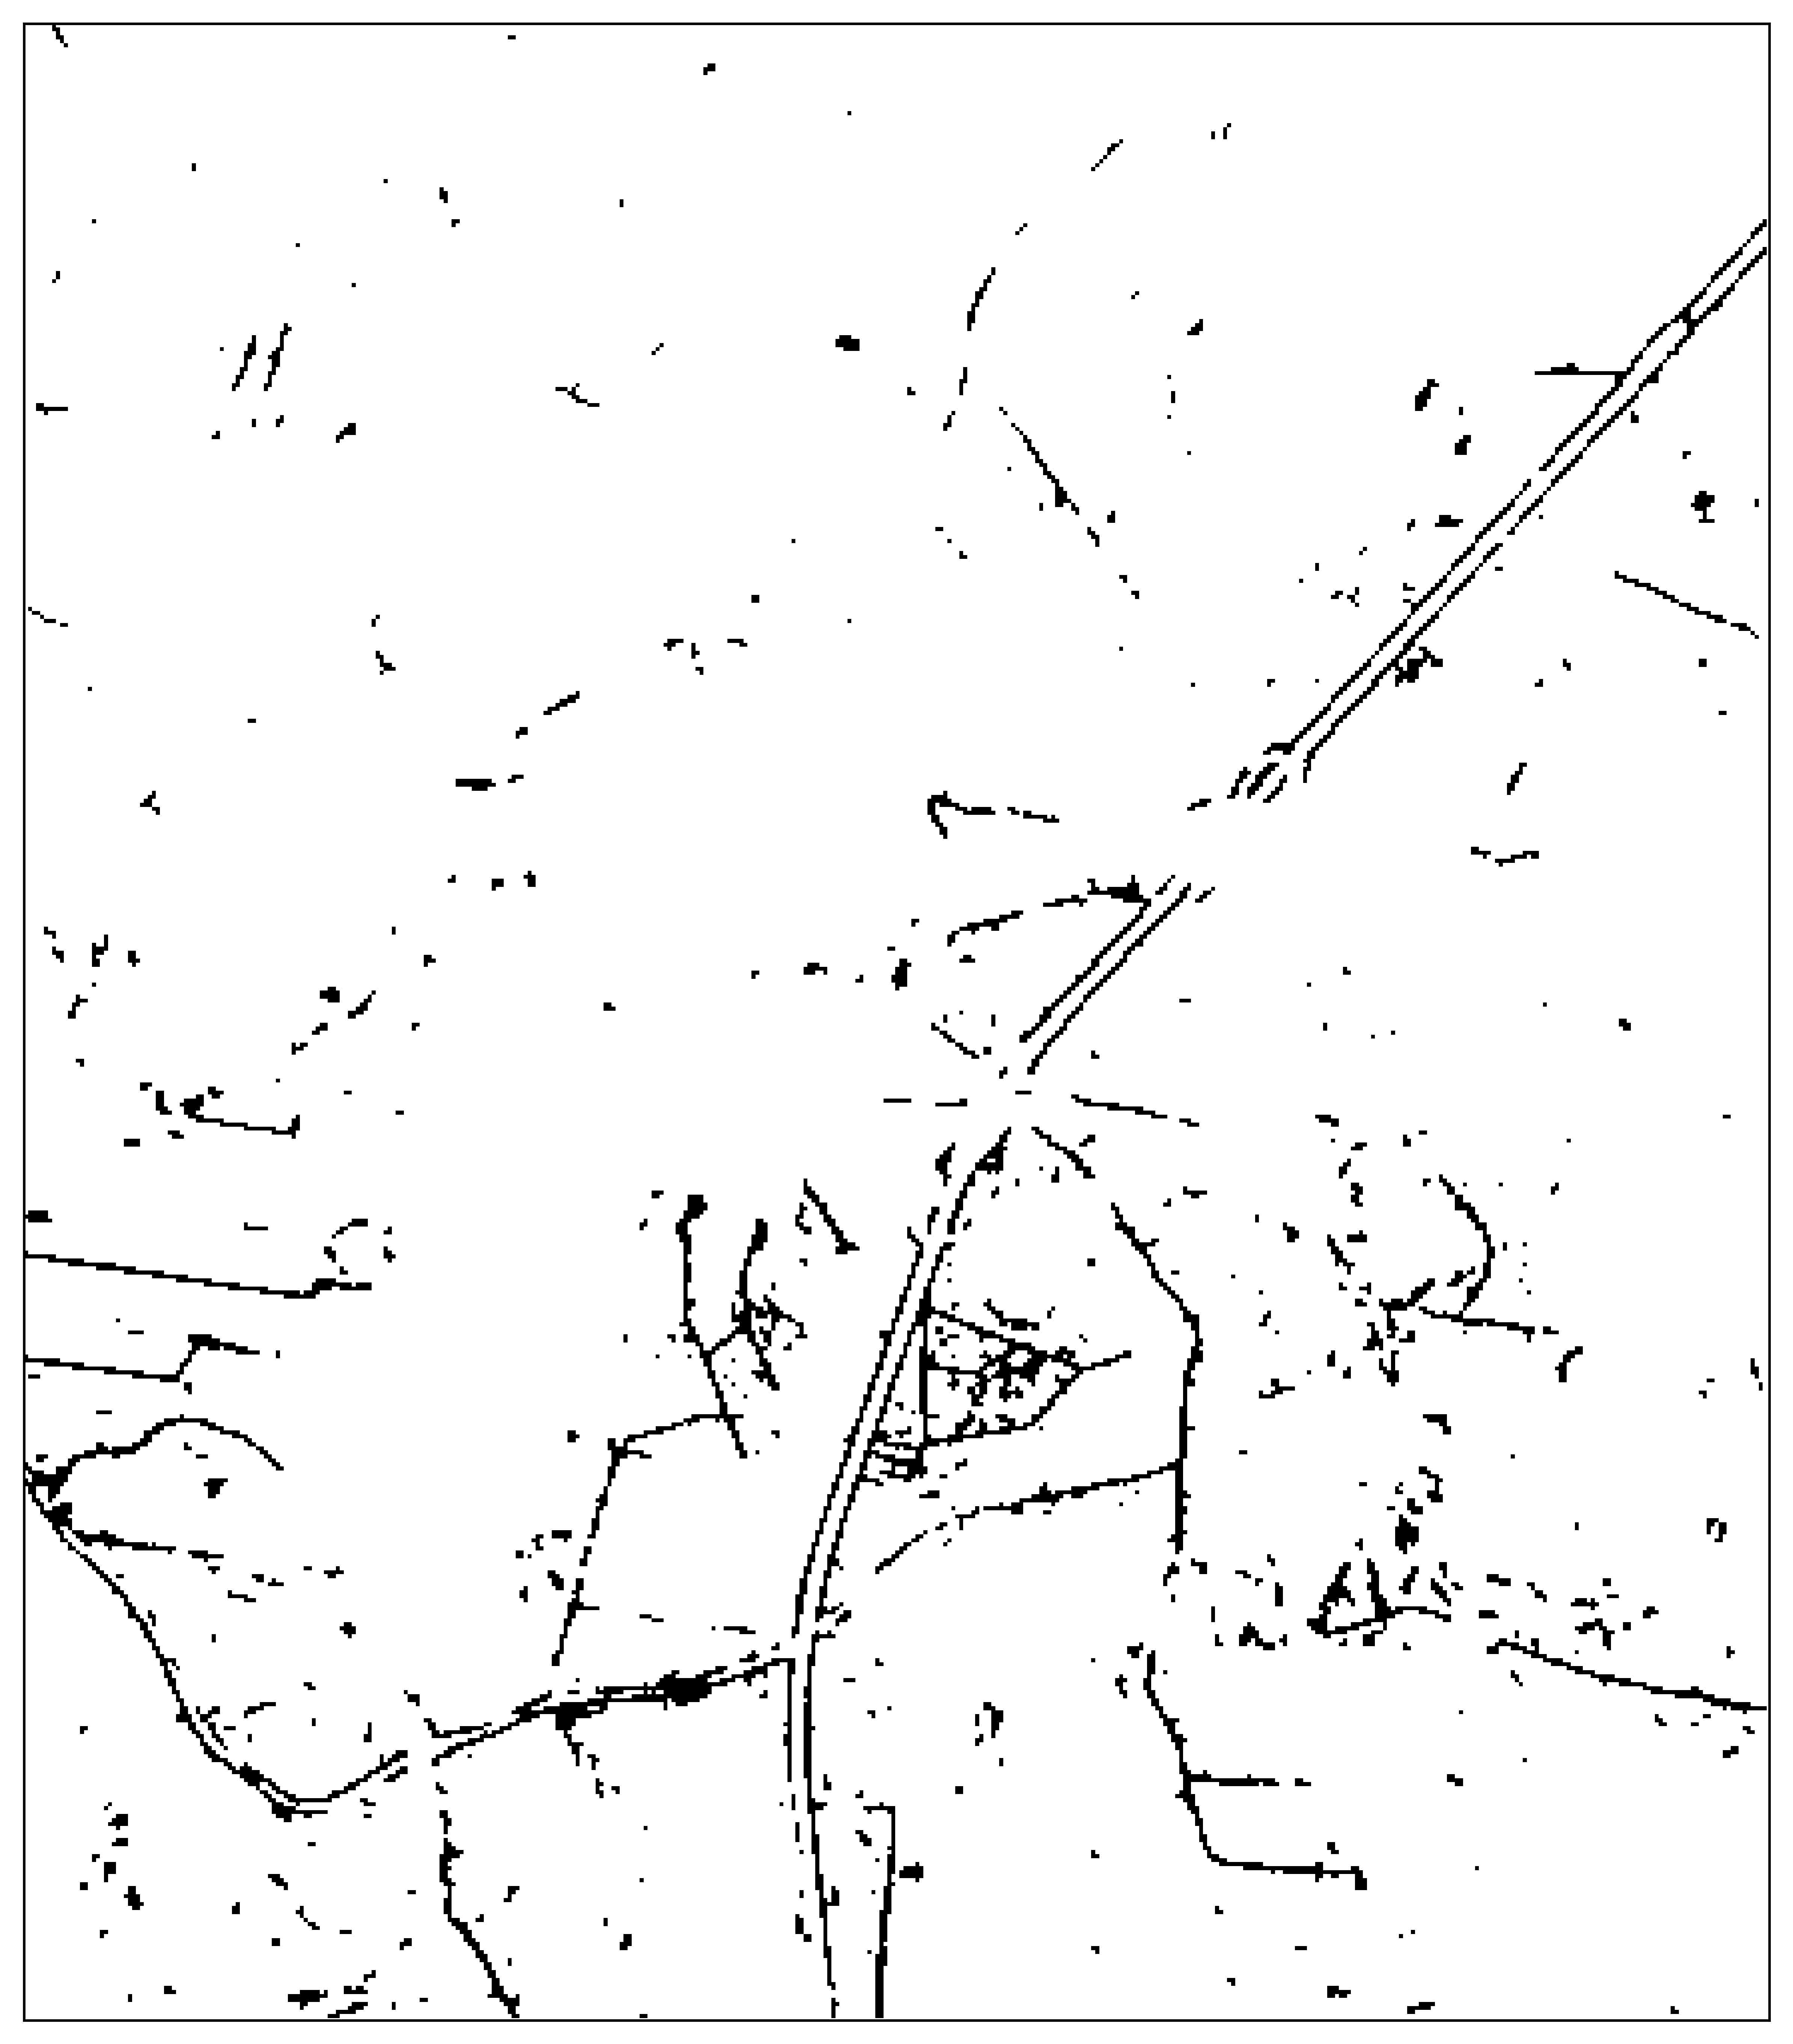
\includegraphics{./images/publ_post_process_step_5_lo.jpg}}}\DIFaddFL{\hspace{5pt}
    }\subfigure[]{
        \resizebox*{5.6cm}{!}{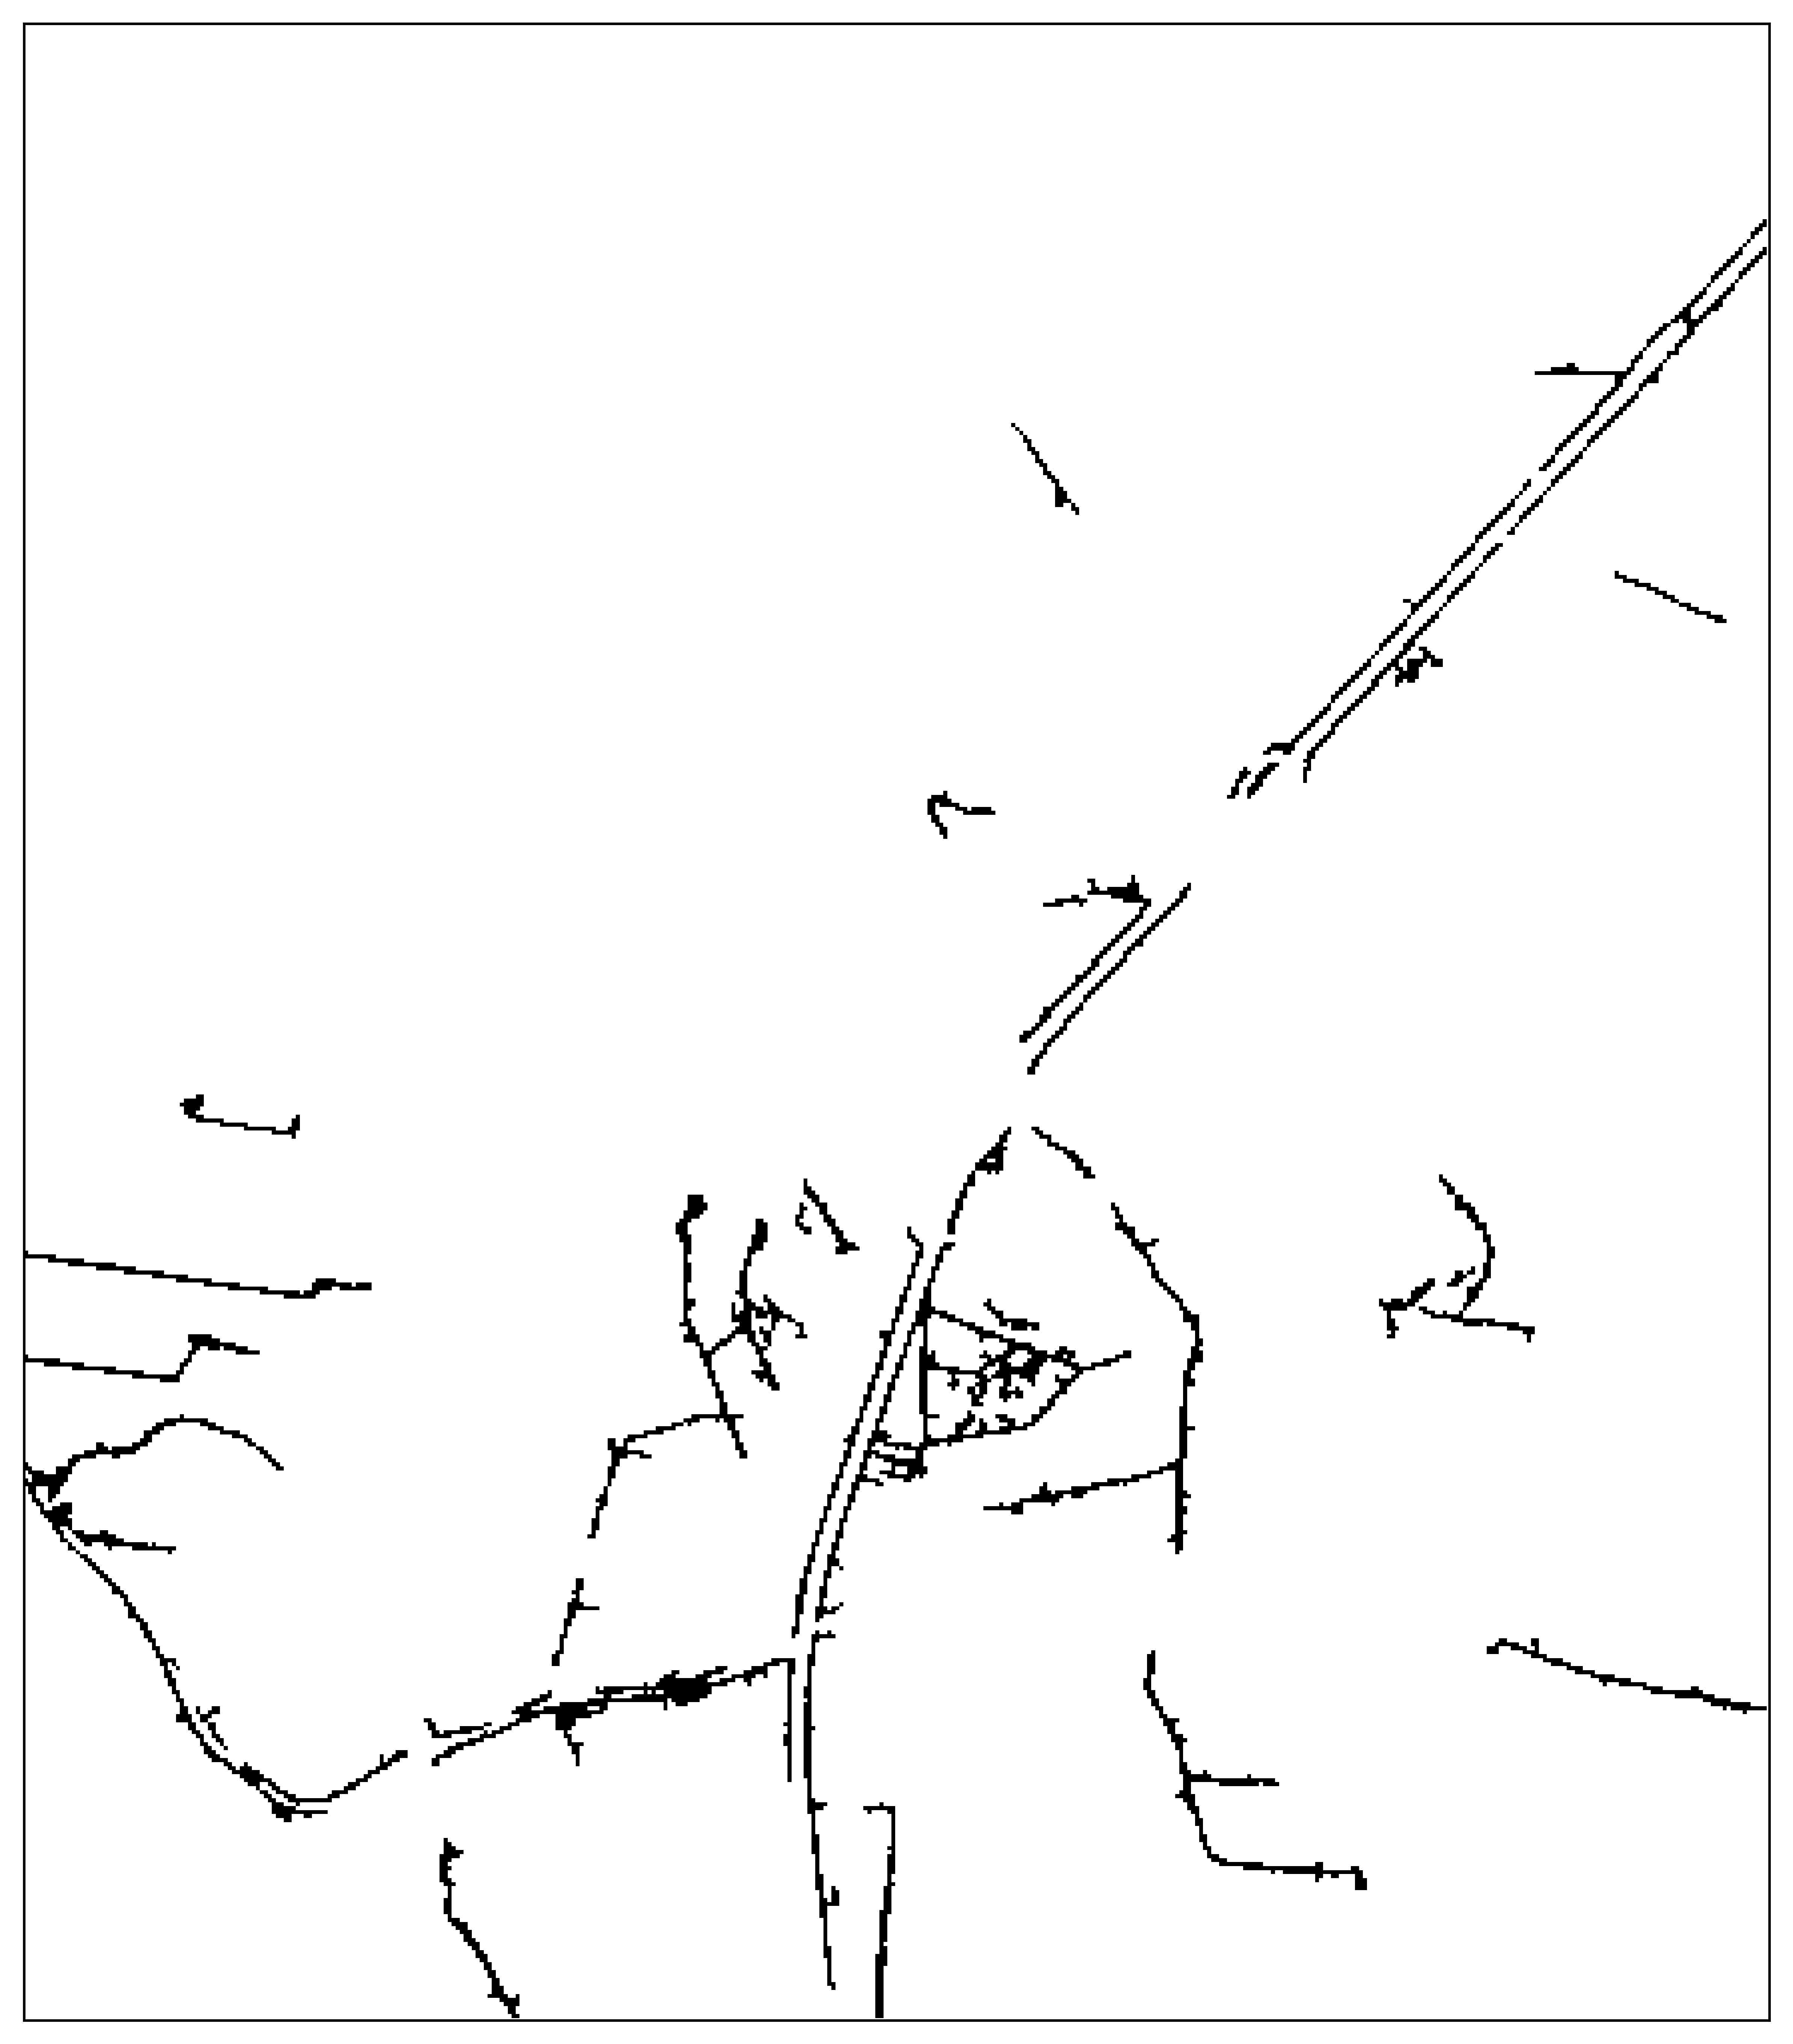
\includegraphics{./images/publ_post_process_step_6_lo.jpg}}}
    \DIFaddendFL \caption{\DIFdelbeginFL \DIFdelFL{Step five and six of the post-process. }\DIFdelendFL \DIFaddbeginFL \textbf{\DIFaddFL{Post-processing step five and six.}} \DIFaddendFL Black pixels indicate a ditch prediction. \textbf{a: }Grid zone binarisation \textbf{b: }Cluster removal \DIFaddbeginFL \DIFaddFL{(final ditch prediction)}\DIFaddendFL .}
    \label{fig:postprocessing3}
\end{figure}

\subsection{Evaluation} \label{evaluation}

Using only accuracy as an evaluation metric when dealing with an imbalanced dataset (roughly 98 \% of all pixels are non-ditch) would produce a poor performance assessment \citep{balanced}; by simply classifying all pixels as non-ditches, we would by default attain 98 \% accuracy. For this reason, the results were mainly evaluated using Cohen's Kappa (Cohen's $\kappa$) index, and the Area under Precision-Recall curve. Cohen's $\kappa$ index measures how much better a prediction is compared to a completely random prediction, where \DIFdelbegin \DIFdel{random would yield a value of zero \mbox{%DIFAUXCMD
\citep{kappa123}}\hspace{0pt}%DIFAUXCMD
. With our data, a $\kappa$ value close to zero would be attained by }\DIFdelend predicting 2 \% of the occurrences as ditch pixels completely at random \DIFaddbegin \DIFadd{would yield a value of zero \mbox{%DIFAUXCMD
\citep{kappa123}}\hspace{0pt}%DIFAUXCMD
}\DIFaddend . Values above zero are better than random, and values below zero are worse than random.

The random rating $P_c$ of a prediction of $n$ occurrences is calculated with:\footnote{ P = Positive (ditch pixel), N = Negative (non-ditch pixel), T = true, F = false}

$$
P_c = \frac{\left(\frac{(TP + FN) \cdot (TP + FP)}{n}\right) + \left(\frac{(FN + TN) \cdot (FP + TN)}{n}\right)}{n}
$$


\DIFdelbegin \begin{displaymath}
\DIFdel{\text{Cohen's } \kappa \text{ is then calculated as a value between -1 and 1 with:}
}\end{displaymath}%DIFAUXCMD
\DIFdelend \DIFaddbegin \DIFadd{Cohen's $\kappa$ is then calculated as a value between -1 and 1 with:
}

\DIFaddend $$\kappa = \frac{Accuracy - P_c}{1 - P_c}$$

The Precision-Recall curve and the Area under Precision-Recall curve (AUPRC) are additional metrics that can be used when evaluating datasets with a largely imbalanced class distribution \citep{precision_recall_curve}. The \DIFdelbegin \DIFdel{Precision-Recall curve has the recall value on the x-axis and the precision value on the y-axis, and the area under the curve that is defined by this point gives the AUPRC value. The area under this curve is given as a value between zero and one, where a value closer to one is better. The }\DIFdelend weighting causes the Precision-Recall curve to \DIFdelbegin \DIFdel{not place an equal value }\DIFdelend \DIFaddbegin \DIFadd{place an unequal weight }\DIFaddend on true negatives and true positives \citep{precision_recall_curve}. For our ditch detection problem, this means that the AUPRC evaluation metric favours accurately classifying ditch pixels over accurately classifying non-ditch pixels.

To circumvent some of the \DIFdelbegin \DIFdel{performance }\DIFdelend evaluation issues arising from the use of pixel classification for ditch objects\DIFaddbegin \DIFadd{, }\DIFaddend as well as not having completely accurate labels on a pixel basis (due to uncertainties in the width of the ditches), we modified the evaluation labels to allow for some error in close proximity to ditches in the prediction. False negative and false positive grid zones that lay adjacent to the ditch label grid zones were evaluated as true negatives and true positives, as they can be considered a part of correctly located ditch objects (\hyperref[fig:newlabels]{Figure} \ref{fig:newlabels}).

\begin{figure} [!htb]
    \centering
    \DIFdelbeginFL %DIFDELCMD < \subfigure[]{
%DIFDELCMD <         \resizebox*{6.5cm}{!}{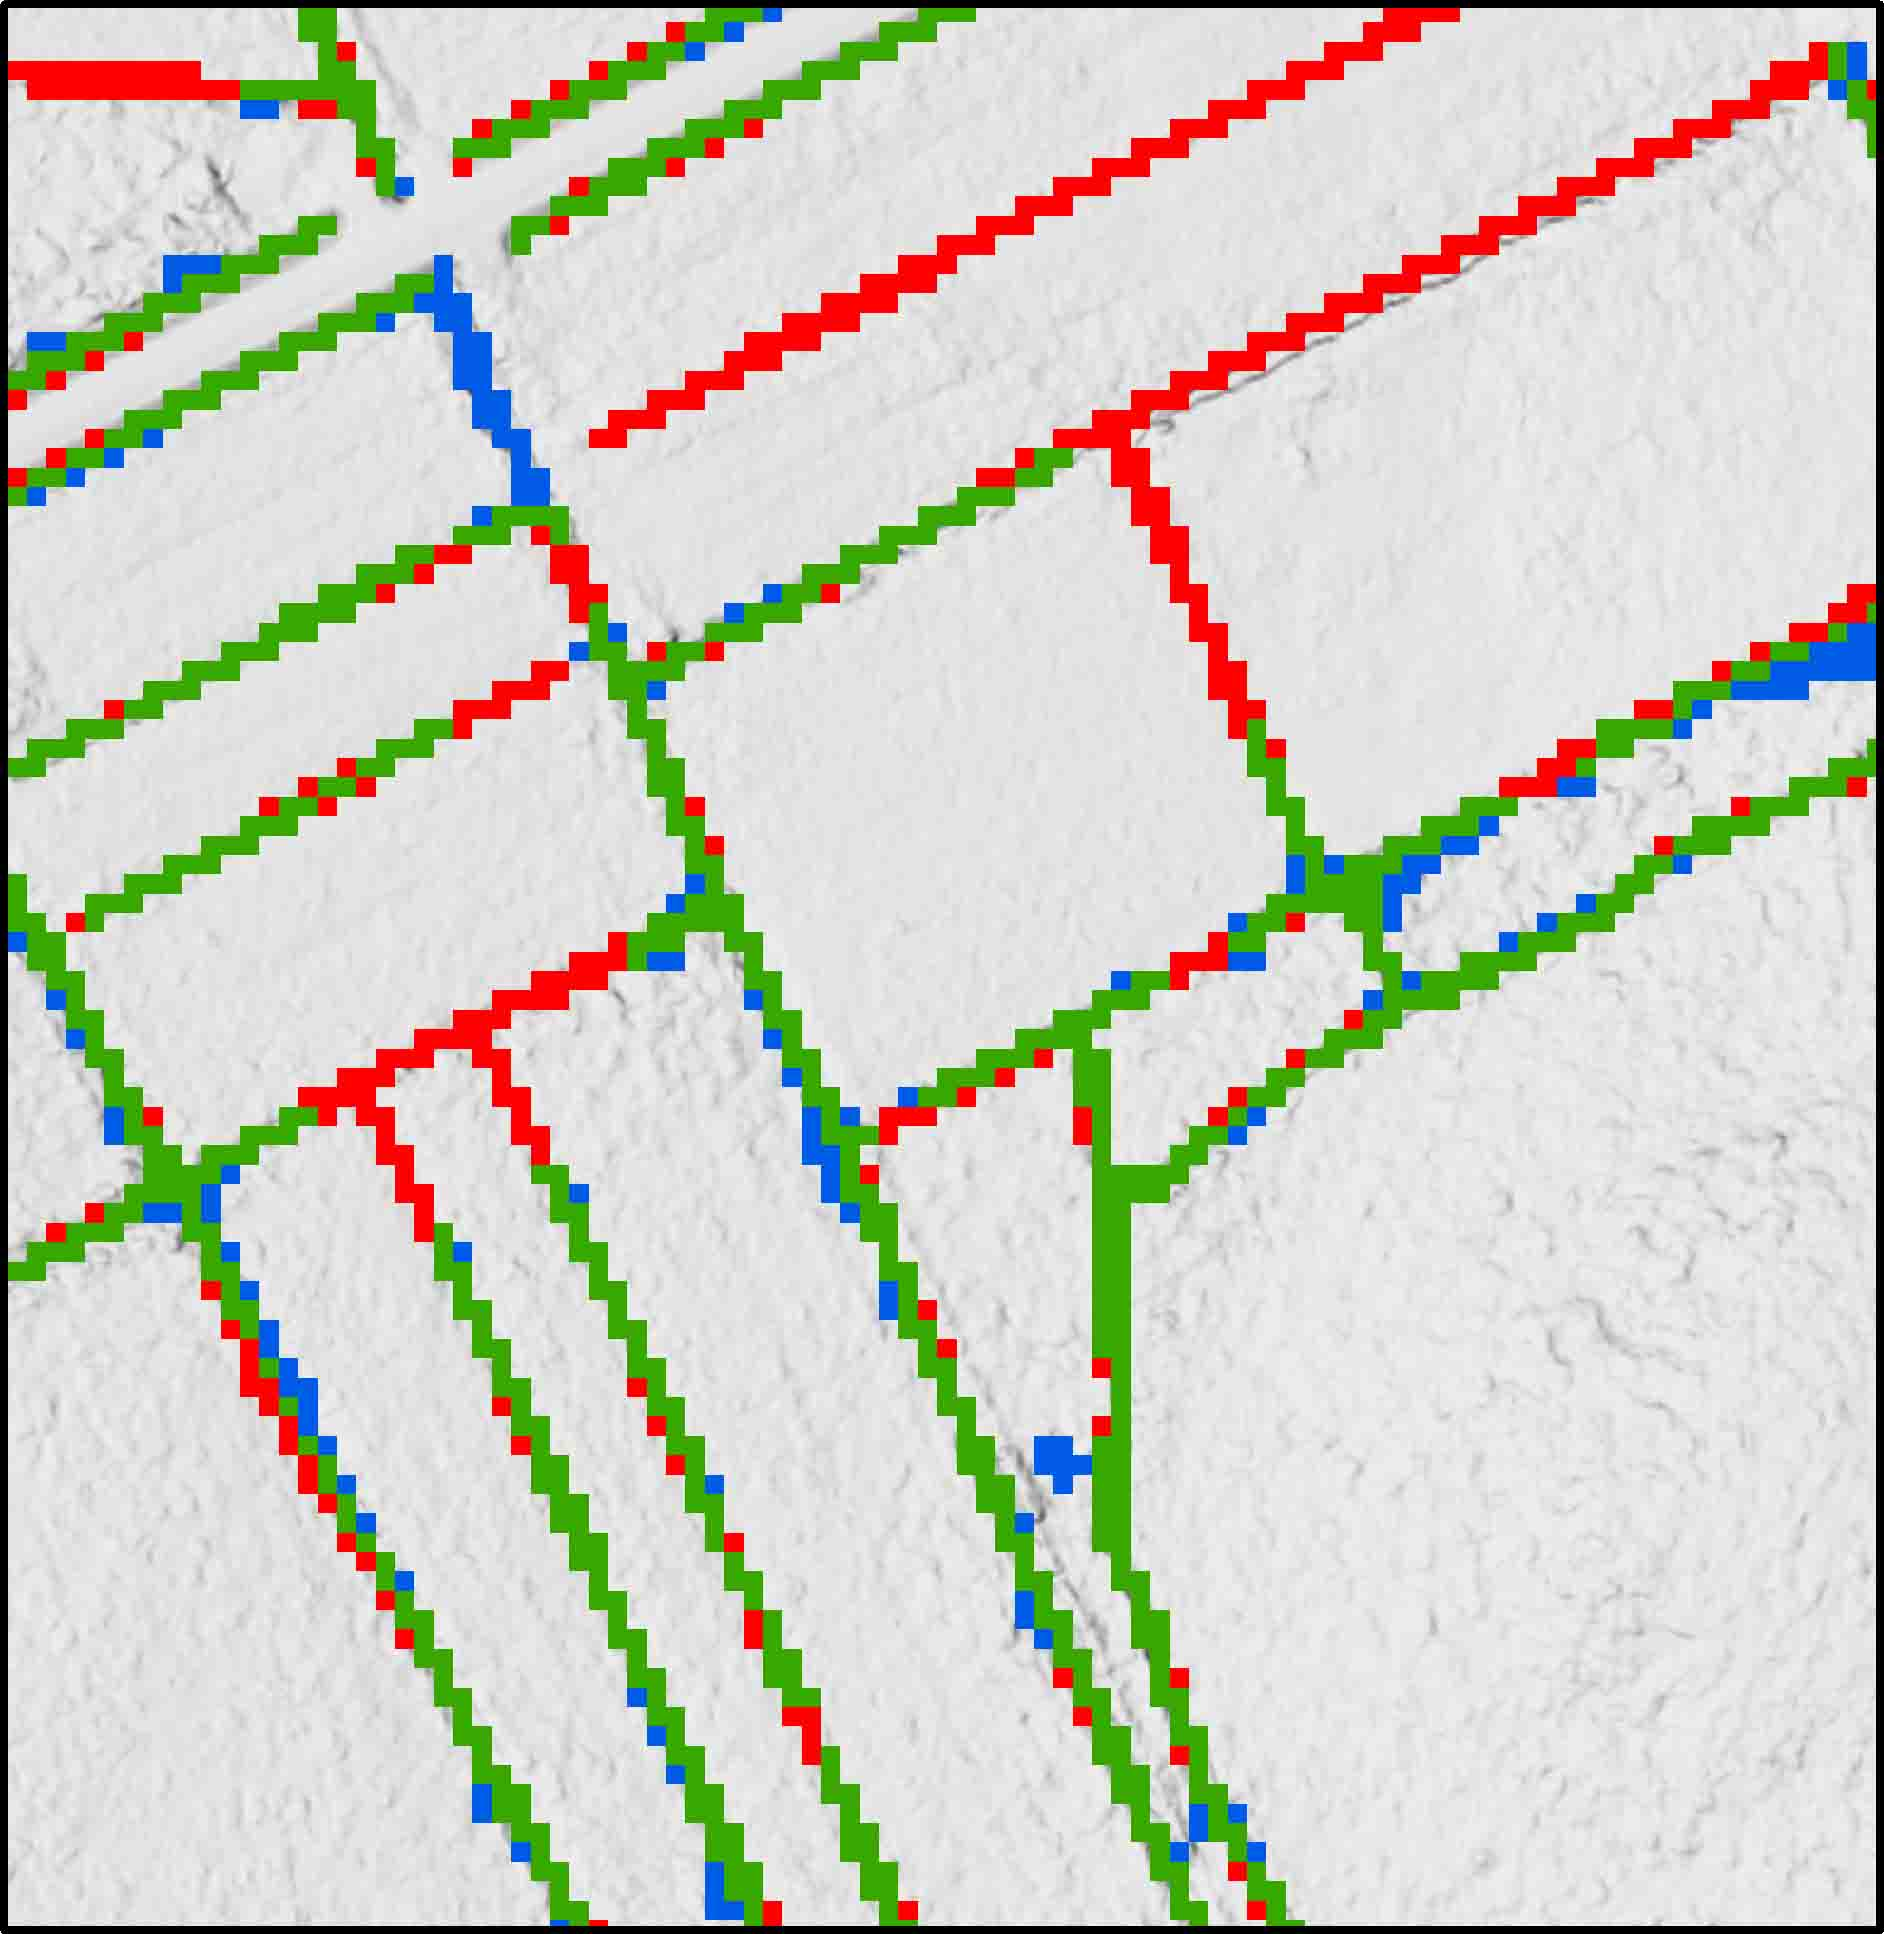
\includegraphics{./images/re_evaluation_1_lo.jpg}}}%%%
\DIFdelFL{\hspace{5pt}
    }%DIFDELCMD < \subfigure[]{
%DIFDELCMD <         \resizebox*{6.5cm}{!}{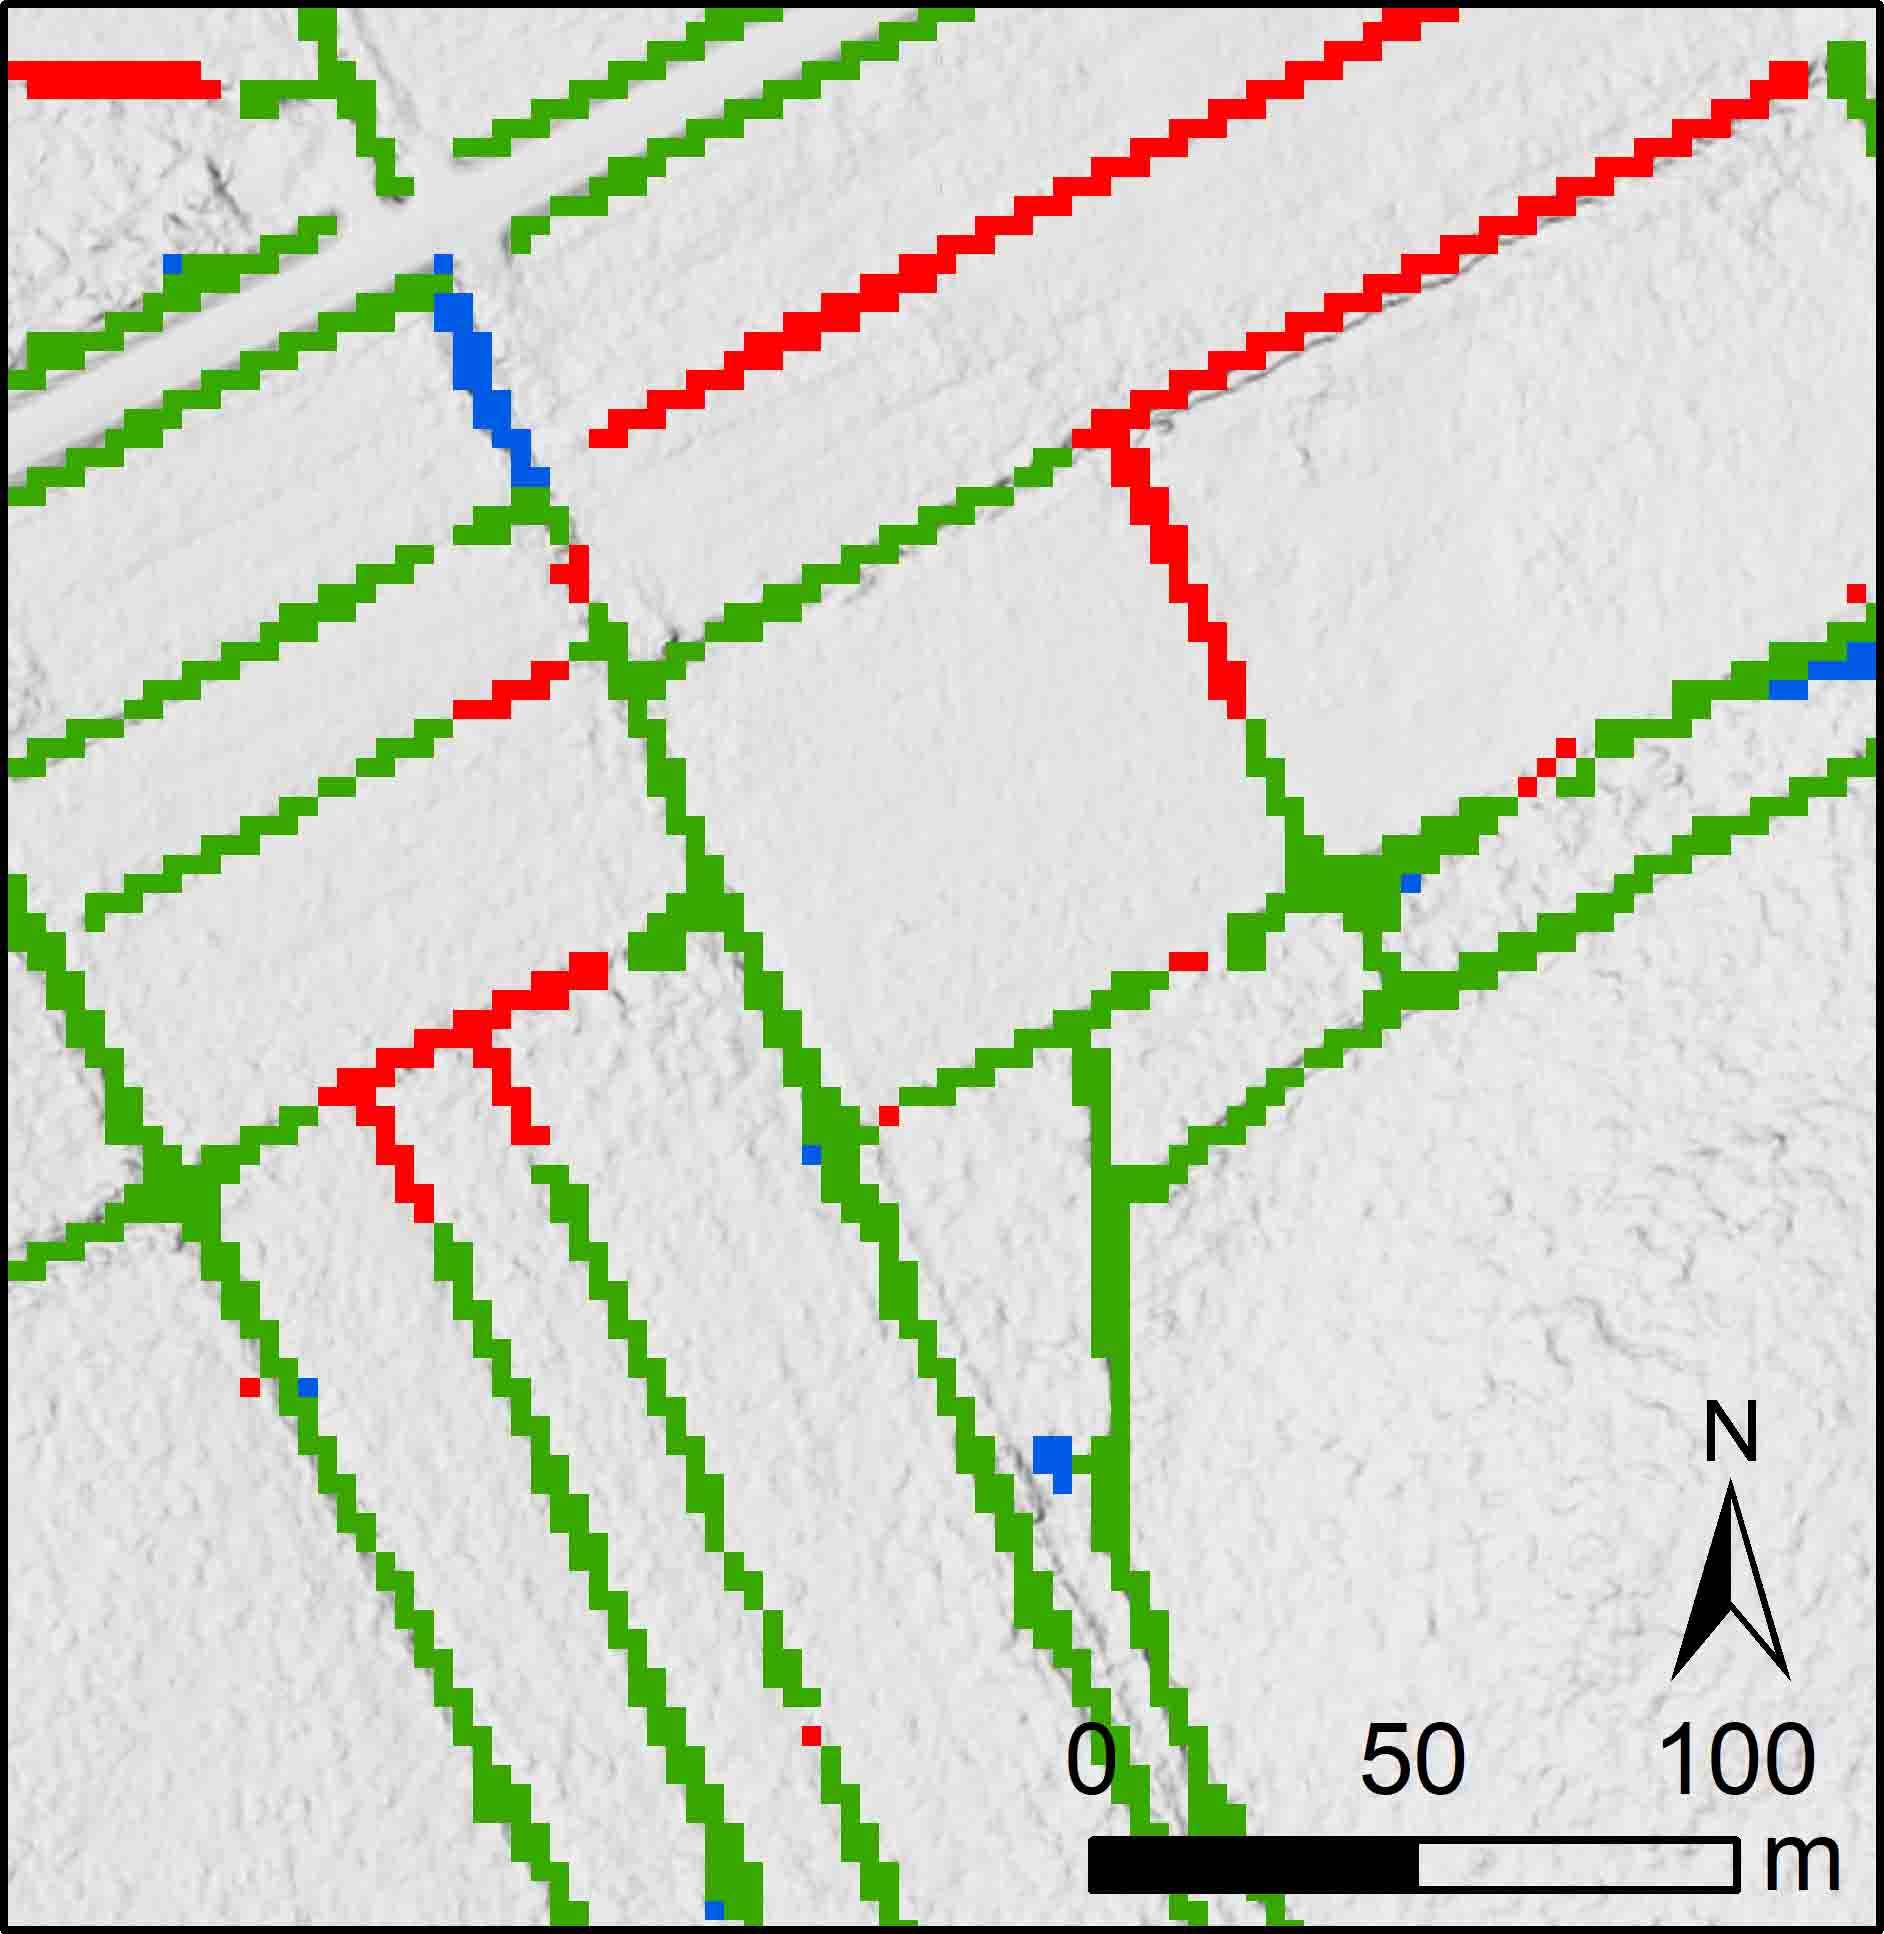
\includegraphics{./images/re_evaluation_2_lo.jpg}}}
%DIFDELCMD <     %%%
\DIFdelendFL \DIFaddbeginFL \subfigure[]{
        \resizebox*{6.65cm}{!}{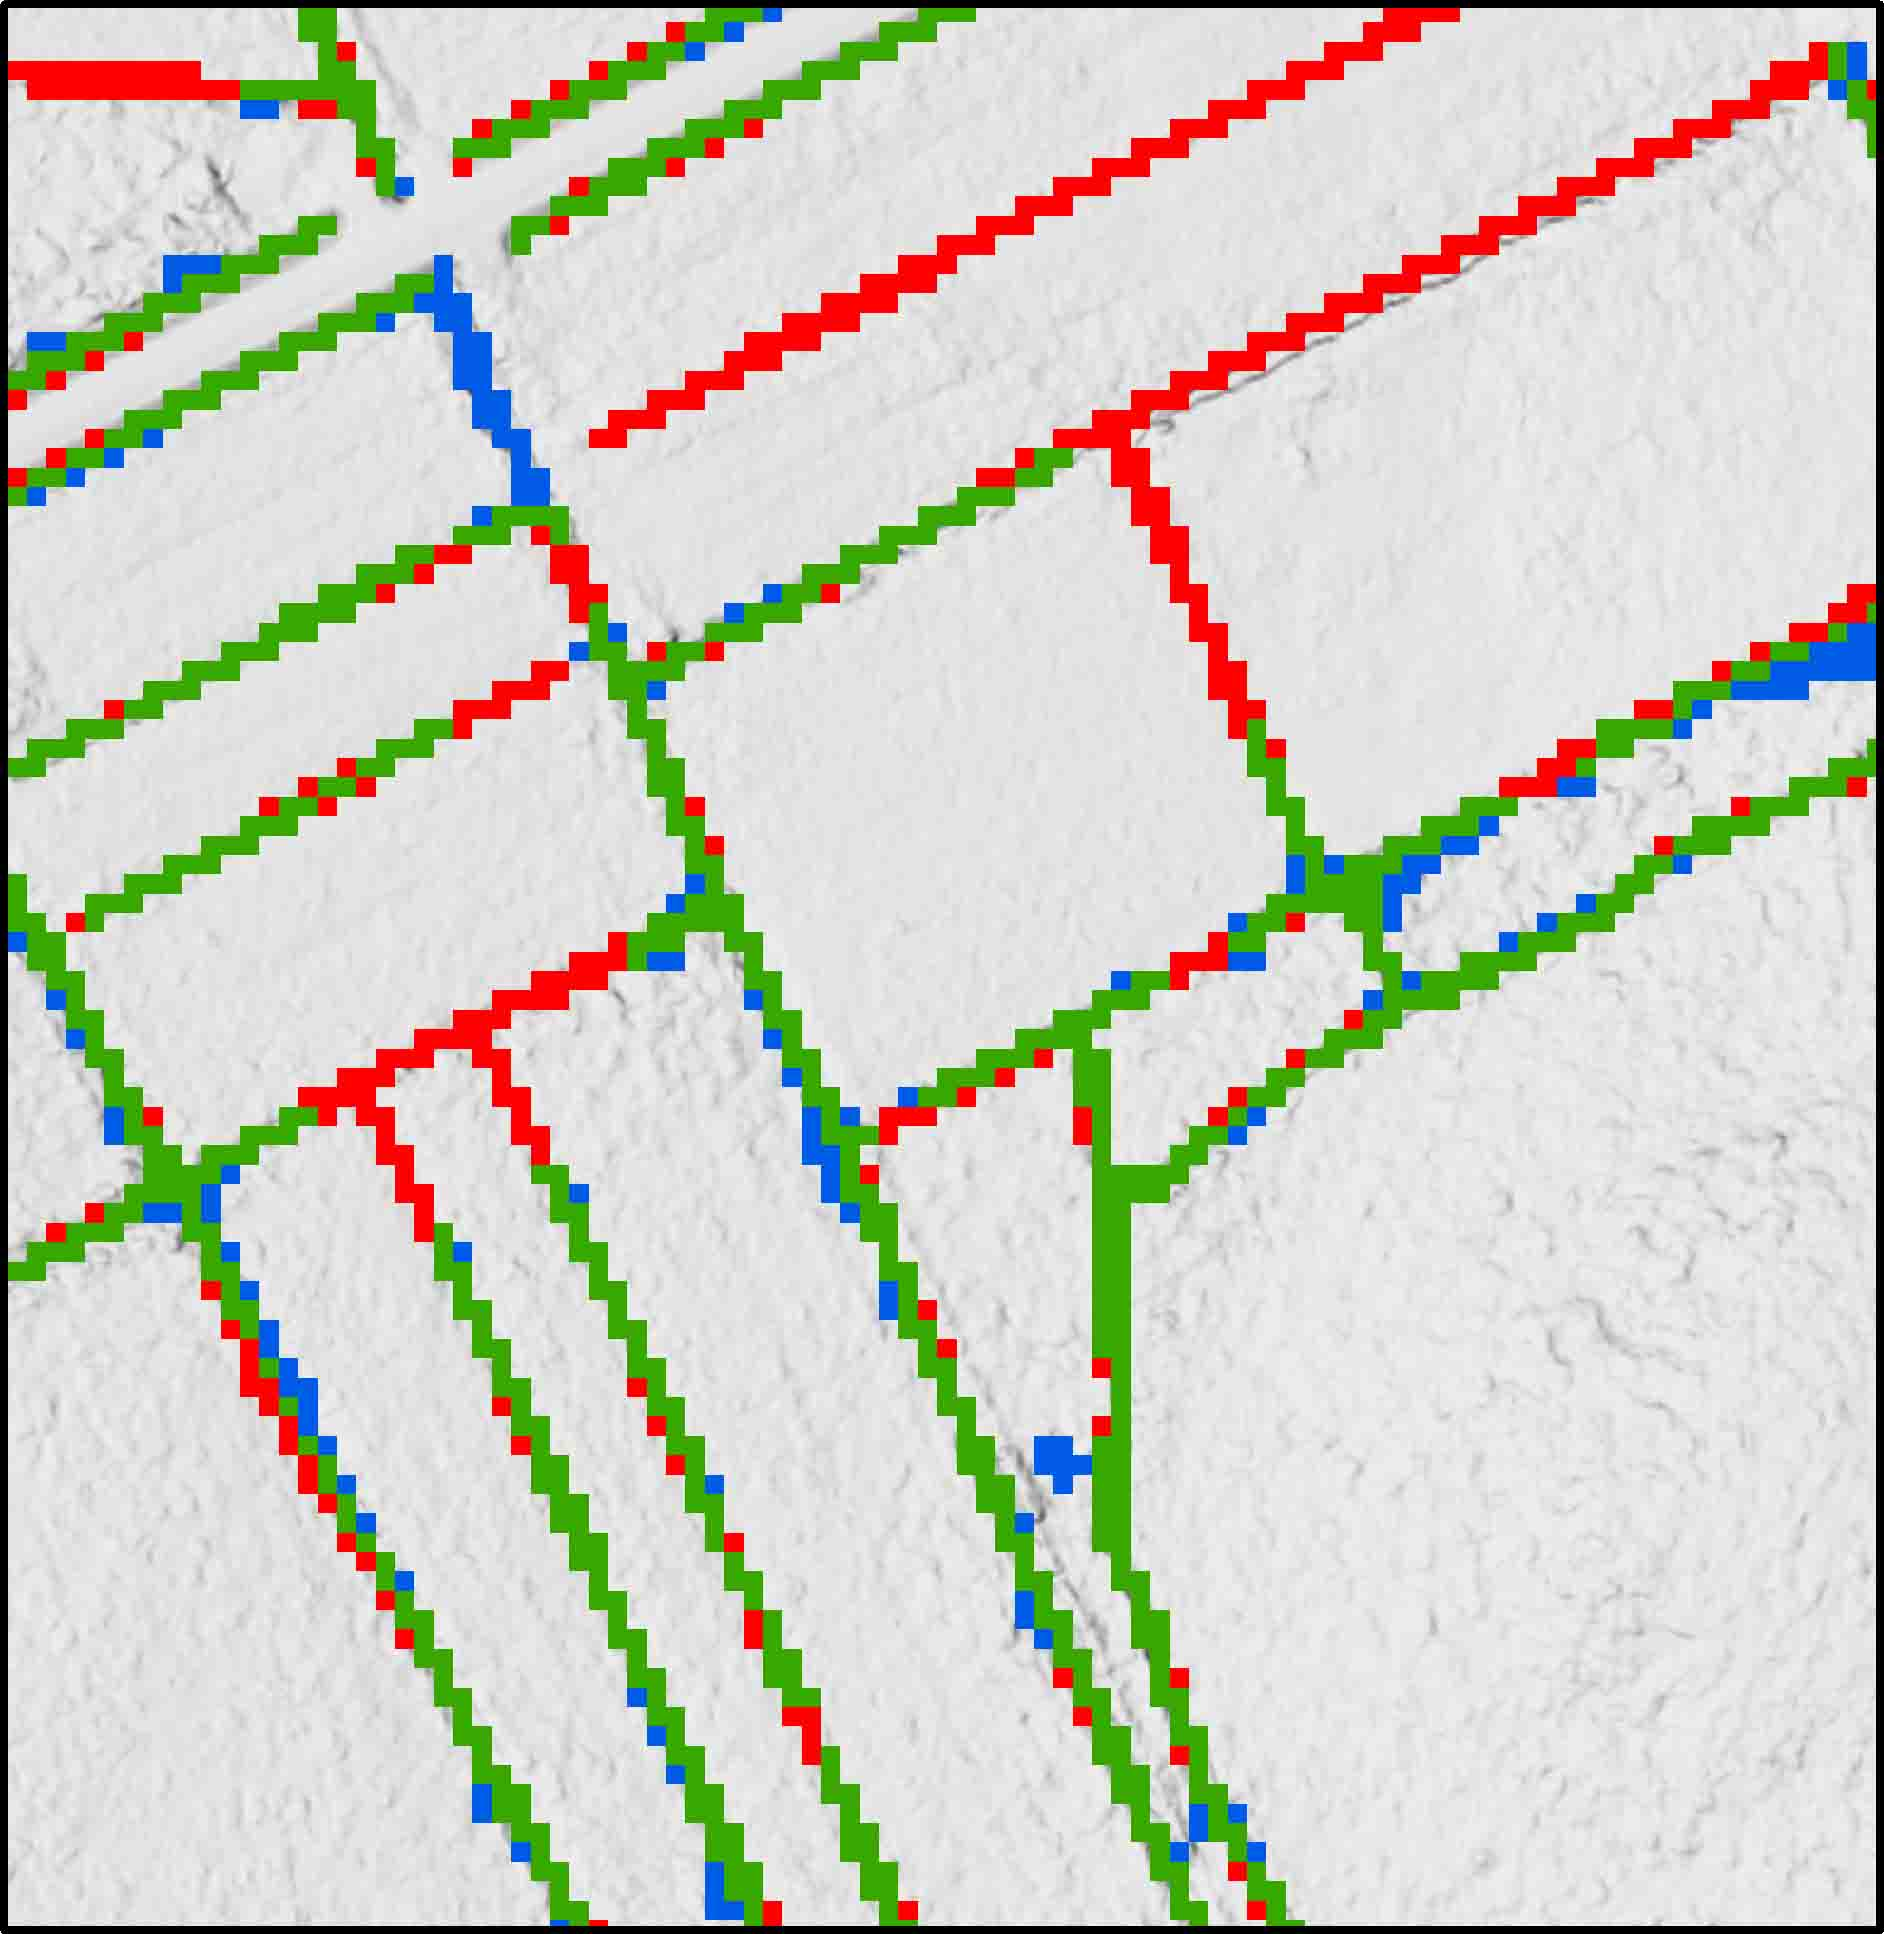
\includegraphics{./images/re_evaluation_1_lo.jpg}}}\DIFaddFL{\hspace{5pt}
    }\subfigure[]{
        \resizebox*{6.65cm}{!}{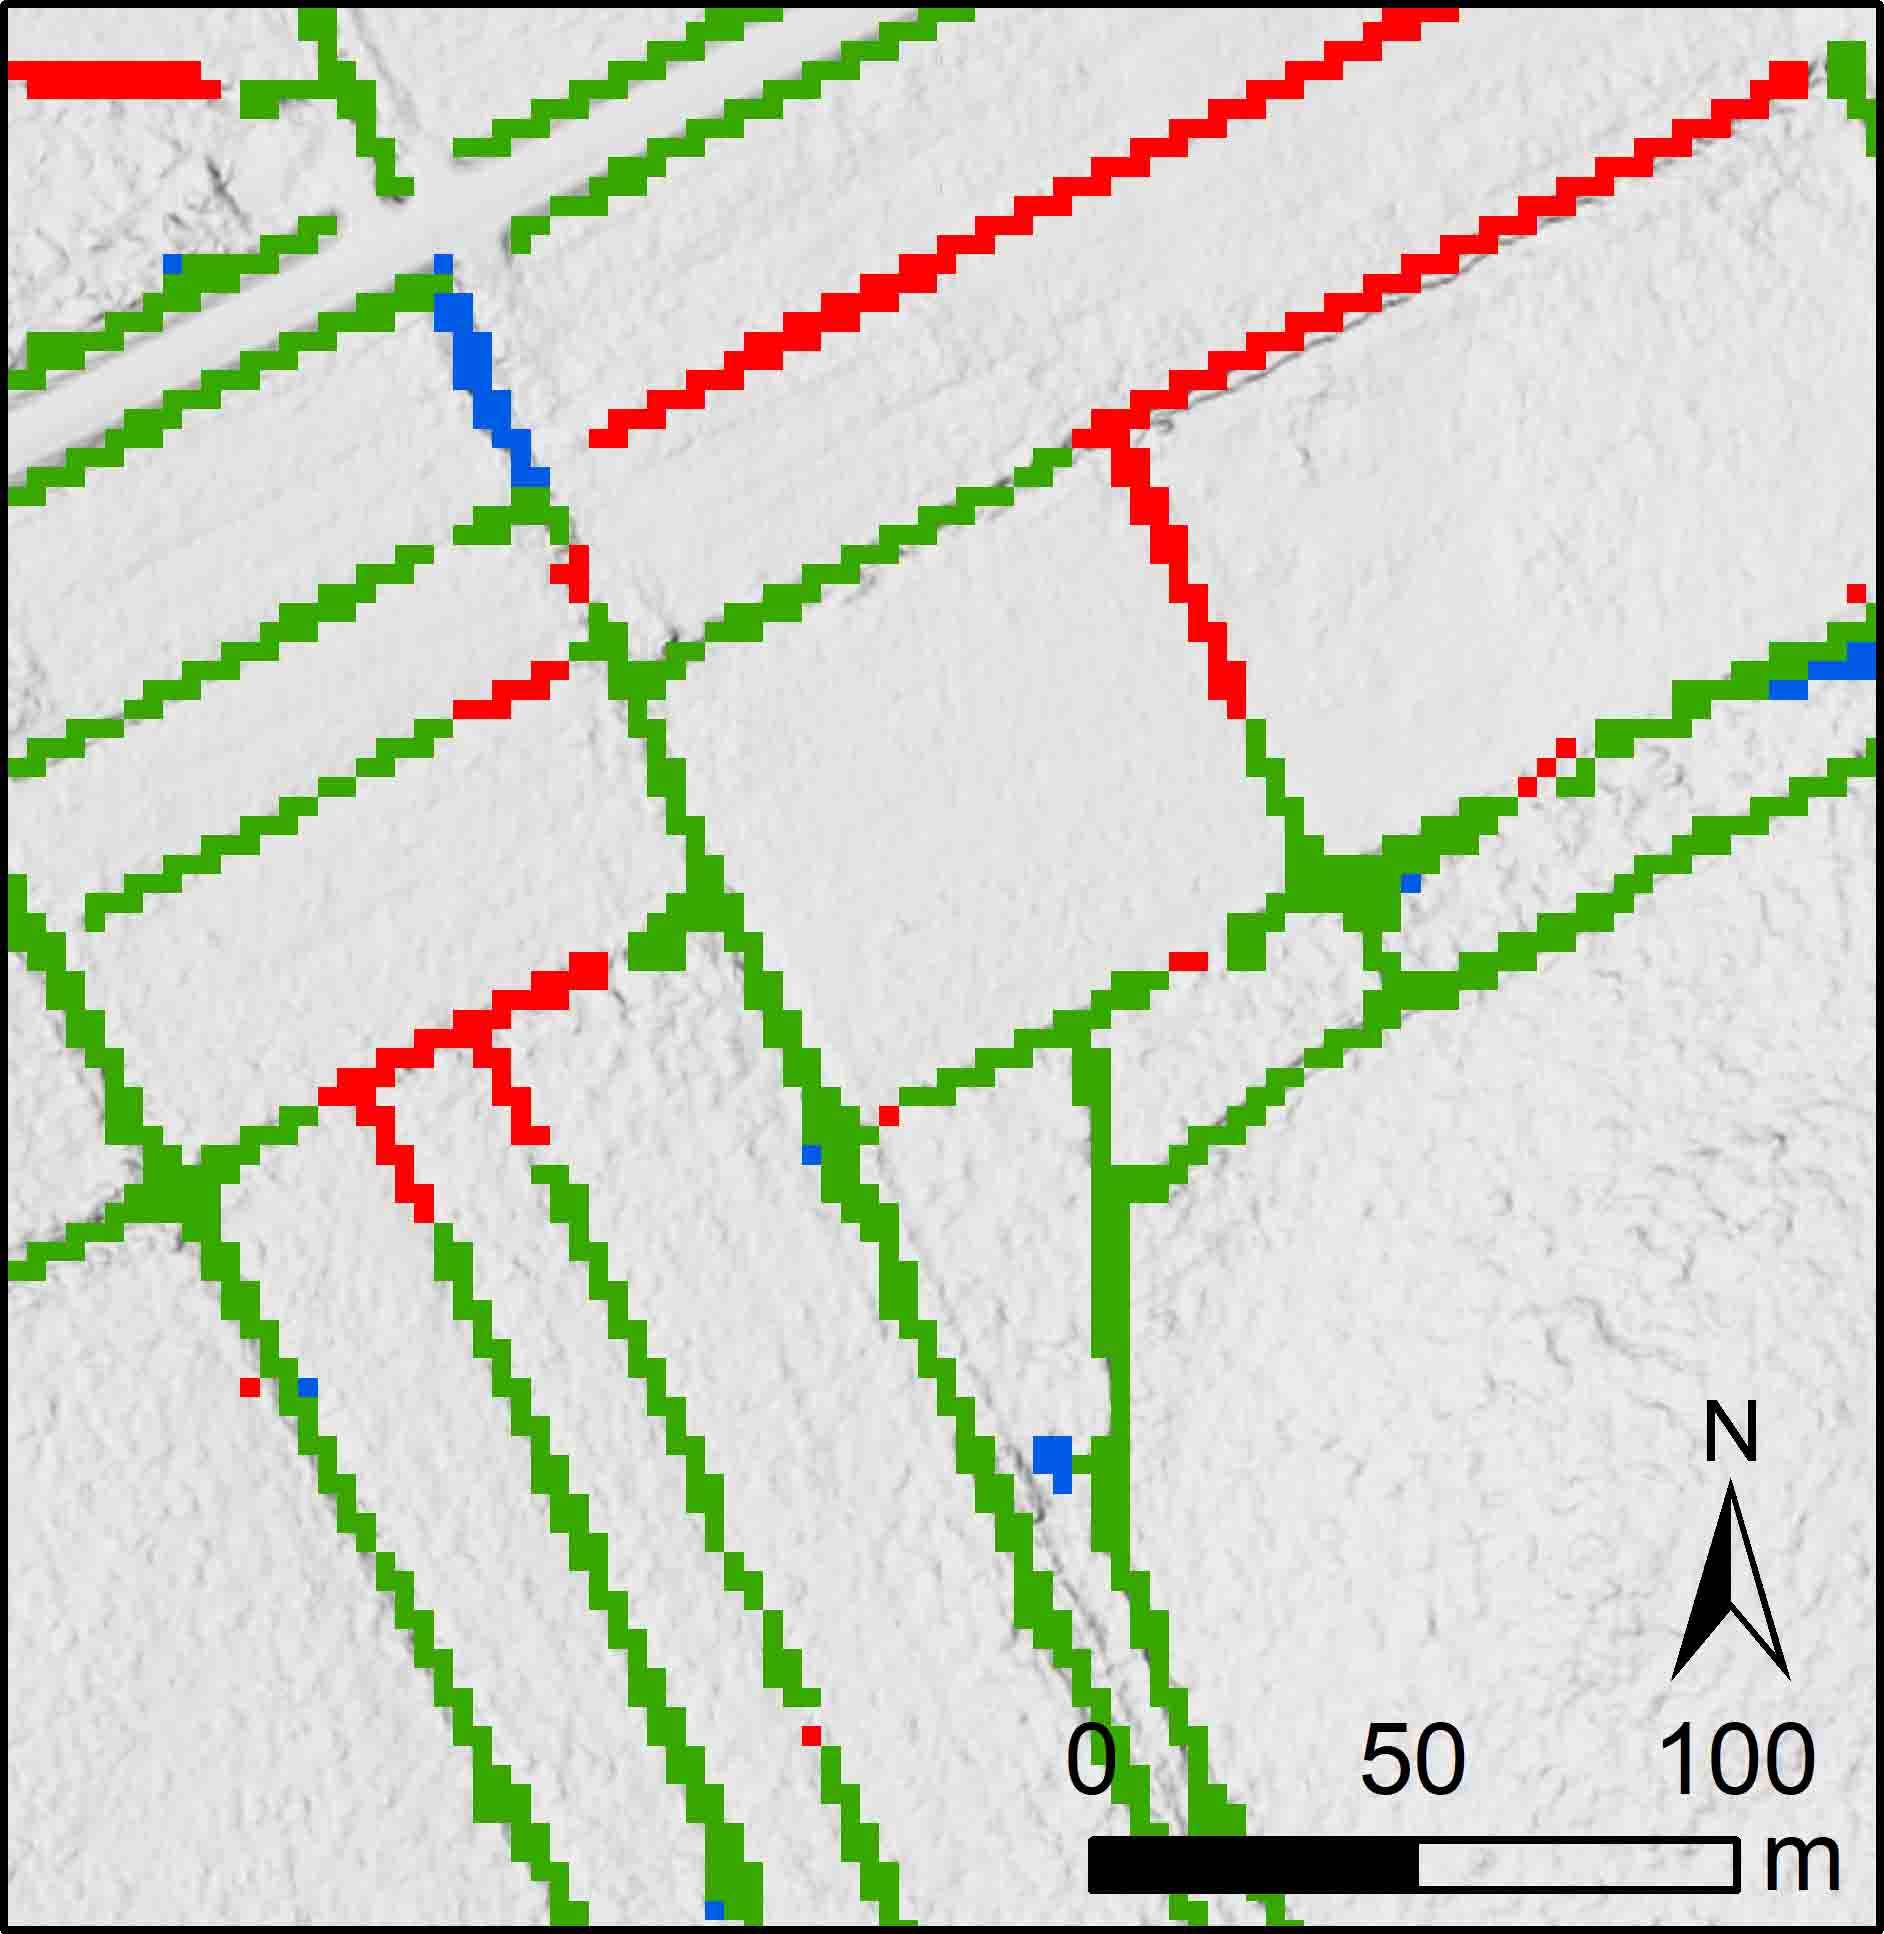
\includegraphics{./images/re_evaluation_2_lo.jpg}}}
    \DIFaddendFL \caption{\DIFdelbeginFL \DIFdelFL{Illustration of the modified evaluation labels. }\DIFdelendFL \DIFaddbeginFL \textbf{\DIFaddFL{Modifying evaluation labels.}} \DIFaddendFL Green marks true positives, red marks false negatives, and blue marks false positives. False positives and false negatives that lay within one grid zone (9 $m^2$) of a ditch label were evaluated as true positives and true negatives. \textbf{a:} Original results, \textbf{b:} Modified results. }
    \label{fig:newlabels}
\end{figure}

\section{Results and analysis}
\DIFdelbegin \DIFdel{In the national survey (NILS), a total of 1103 natural watercourses, 131 straightened watercourses/channels, and 2089 ditches were found in the field. This simple investigation highlights two things: Firstly, the ditches make up the majority of the small scale water channels in the Swedish landscape; almost twice as many as the natural streams. Secondly, most of the small scale channels are missing on the current maps; only 45 \% of the natural watercourses, 25 \% of the straightened watercourses/channels, and 9 \% of the ditches were mapped (}%DIFDELCMD < \hyperref[fig:watercoursebarplot]{Figure} %%%
\DIFdel{\ref{fig:watercoursebarplot}).
}\DIFdelend 

\DIFdelbegin %DIFDELCMD < \begin{figure}[!htb]
%DIFDELCMD <     \centering
%DIFDELCMD <     \begin{tikzpicture}
%DIFDELCMD <     \begin{axis}[
%DIFDELCMD <         width={0.9\textwidth},
%DIFDELCMD <         height={0.6\textwidth},
%DIFDELCMD <         ylabel={fluorescence},
%DIFDELCMD <         ybar stacked,
%DIFDELCMD <         ymajorgrids=true,
%DIFDELCMD <     	bar width=45pt,
%DIFDELCMD <     	nodes near coords,
%DIFDELCMD <     	every node near coord/.append style={font=\tiny},
%DIFDELCMD <         enlarge y limits={0.15},
%DIFDELCMD <         enlarge x limits=0.15,
%DIFDELCMD <         legend style={at={(0.78,0.96)},
%DIFDELCMD <           anchor=north,legend columns=-1},
%DIFDELCMD <         ylabel={{}},
%DIFDELCMD <         symbolic x coords={Ditches, Straightened  watercourses, Natural  watercourses},
%DIFDELCMD <         xtick=data,
%DIFDELCMD <         ytick={0,500,1000,1500,2000},
%DIFDELCMD <         x tick label style={rotate=0,anchor=north},
%DIFDELCMD <         ]
%DIFDELCMD <     \addplot+[ybar,color=custombeige,fill=custombeige,draw=custombeigeouter,thick] plot coordinates {(Ditches,188) (Straightened  watercourses,33) 
%DIFDELCMD <       (Natural  watercourses,496)};
%DIFDELCMD <     \addplot+[ybar,color=customgrayouter,fill=customgray,draw=customgrayouter,thick] plot coordinates {(Ditches,1901) (Straightened  watercourses,98) 
%DIFDELCMD <       (Natural  watercourses,607)};
%DIFDELCMD <     \legend{\strut Mapped, \strut Unmapped}
%DIFDELCMD <     \end{axis}
%DIFDELCMD <     \end{tikzpicture}
%DIFDELCMD <     %%%
%DIFDELCMD < \caption{%
{%DIFAUXCMD
\DIFdelFL{The bars indicate the number of observed channels in the National Inventory of Landscapes in Sweden's (NILS) line inventory of small watercourses (width $<$ 6 m). The colours of the bars indicate if they are mapped or not on the Swedish Property map.}}
    %DIFAUXCMD
%DIFDELCMD < \label{fig:watercoursebarplot}
%DIFDELCMD < \end{figure}
%DIFDELCMD < 

%DIFDELCMD < %%%
\DIFdelend \hyperref[recreatedpredictionperformance]{Table} \ref{recreatedpredictionperformance} shows the evaluation metrics from the experiments \DIFdelbegin \DIFdel{with }\DIFdelend \DIFaddbegin \DIFadd{where }\DIFaddend the digital terrain indices \DIFaddbegin \DIFadd{were thresholded }\DIFaddend separately. Of the four, the \DIFdelbegin \DIFdel{Impoundment Index and the HPMF index }\DIFdelend \DIFaddbegin \hyperref[impoundment]{Impoundment Index} \DIFadd{and }\hyperref[hpmf]{HPMF} \DIFaddend performed relatively close to each other\DIFaddbegin \DIFadd{, }\DIFaddend and outperformed the other indices for most of the metrics.

\begin{table}[!htb]
\DIFdelbeginFL %DIFDELCMD < \tbl{Metrics from the total results of the four digital terrain indices experiments.}
%DIFDELCMD <     %%%
\DIFdelendFL \DIFaddbeginFL \centering
    \DIFaddendFL {\begin{tabular}{lcccc}
        \DIFdelbeginFL %DIFDELCMD < \toprule
%DIFDELCMD <         %%%
\DIFdelFL{Metric }\DIFdelendFL \DIFaddbeginFL \textbf{\DIFaddFL{Metric}} \DIFaddendFL & \DIFdelbeginFL \DIFdelFL{Sky View Factor }\DIFdelendFL \DIFaddbeginFL \textbf{\hyperref[skyviewfactor]{Sky View Factor}} \DIFaddendFL & \DIFdelbeginFL \DIFdelFL{Impoundment }\DIFdelendFL \DIFaddbeginFL \textbf{\hyperref[impoundment]{Impoundment}} \DIFaddendFL & \DIFdelbeginFL \DIFdelFL{HPMF }\DIFdelendFL \DIFaddbeginFL \textbf{\hyperref[hpmf]{HPMF}} \DIFaddendFL & \DIFdelbeginFL \DIFdelFL{Slope}\DIFdelendFL \DIFaddbeginFL \textbf{\hyperref[slope]{Slope}}\DIFaddendFL \\
        \DIFdelbeginFL %DIFDELCMD < \midrule
%DIFDELCMD <         %%%
\DIFdelendFL \DIFaddbeginFL \hline
        \DIFaddendFL Accuracy \%     & 83.67 & 97.07 & 97.45 & 82.66 \\
        Recall \%       & 44.54 & 29.98 & 25.31 & 34.83 \\
        Precision \%    &{ 4.00}  & 18.51 & 20.10 & { 2.99} \\
        $\kappa$ rating & 0.048 & 0.215 & 0.211 & 0.029 \\
        AUPRC & 0.247 & 0.248 & 0.232 & 0.194 \\
        \DIFdelbeginFL %DIFDELCMD < \bottomrule
%DIFDELCMD <     %%%
\DIFdelendFL \DIFaddbeginFL \hline
    \DIFaddendFL \end{tabular}}
    \DIFaddbeginFL \caption{\textbf{\DIFaddFL{Index thresholding metrics.}} \DIFaddFL{Metrics from the total results of the four digital terrain indices experiments, where only a sole terrain index is used with a threshold to detect ditches.}}
    \DIFaddendFL \label{recreatedpredictionperformance}
\end{table}

\hyperref[predictionperformance]{Table} \ref{predictionperformance} displays all the evaluation metrics for the prediction of our \DIFdelbegin \DIFdel{method}\DIFdelend \DIFaddbegin \DIFadd{ditch detector}\DIFaddend . The confidence intervals were calculated from the \DIFaddbegin \DIFadd{results from the }\DIFaddend 11 \DIFdelbegin \DIFdel{different subsectionsthat the experiment was performed on}\DIFdelend \DIFaddbegin \DIFadd{cross-validation subsections}\DIFaddend . Because the subsections have varying amounts of ditches in them, the confidence intervals will not be completely \DIFdelbegin \DIFdel{accurate}\DIFdelend \DIFaddbegin \DIFadd{conclusive}\DIFaddend , but will produce a close estimation. \DIFdelbegin %DIFDELCMD < 

%DIFDELCMD < %%%
\DIFdel{From }%DIFDELCMD < \hyperref[predictionperformance]{Table} %%%
\DIFdel{\ref{predictionperformance}, it is observed that averaging }\DIFdelend \DIFaddbegin \DIFadd{Averaging }\DIFaddend the results from the 11 subsections \DIFdelbegin \DIFdel{would yield }\DIFdelend \DIFaddbegin \DIFadd{yields }\DIFaddend a very similar value to the total results, indicating that the ditch detector generally performs equally well on subsections with a small amount of ditches as on subsections with a large amount of ditches.

\begin{table}[!htb]
\DIFdelbeginFL %DIFDELCMD < \tbl{Metrics for the prediction performance of our ditch detector.}{\begin{tabular}{lccc} 
%DIFDELCMD <         \toprule
%DIFDELCMD <         Metric & Total\textsuperscript{a} & Subsection\textsuperscript{b}& CI 95\%\textsuperscript{c} \\ 
%DIFDELCMD <         &&Average&\\ \midrule
%DIFDELCMD <         Accuracy     \% & 99.00 & 99.00 & [98.69 , 99.32] \\
%DIFDELCMD <         Recall       \% & 70.28 & 70.19 & [61.28 , 79.09] \\
%DIFDELCMD <         Precision    \% & 77.38 & 75.79 & [71.94 , 79.64] \\
%DIFDELCMD <         $\kappa$ rating & 0.732 & 0.718 & [0.655 , 0.781] \\
%DIFDELCMD <         AUPRC           & 0.741 & 0.733 & [0.674 , 0.791] \\ 
%DIFDELCMD <         \bottomrule
%DIFDELCMD <     \end{tabular}}
%DIFDELCMD <     \tabnote{
%DIFDELCMD <         \textsuperscript{a} The result of all 11 subsection experiments when combined. \newline
%DIFDELCMD <         \textsuperscript{b} An average score from the 11 different subsections that the experiment was performed on. \newline
%DIFDELCMD <         \textsuperscript{c} Confidence intervals at 95 \% confidence level.}
%DIFDELCMD <     %%%
\DIFdelendFL \DIFaddbeginFL \centering
    {\begin{tabular}{lccc}
        \textbf{\DIFaddFL{Metric}} & \textbf{\DIFaddFL{Total}}\DIFaddFL{\textsuperscript{a} }& \textbf{\DIFaddFL{Subsection Average}}\DIFaddFL{\textsuperscript{b}}& \textbf{\DIFaddFL{CI 95\%}}\DIFaddFL{\textsuperscript{c} }\\ 
        \hline
        \DIFaddFL{Accuracy     \% }& \DIFaddFL{99.00 }& \DIFaddFL{99.00 }& [\DIFaddFL{98.69 , 99.32}] \\
        \DIFaddFL{Recall       \% }& \DIFaddFL{70.28 }& \DIFaddFL{70.19 }& [\DIFaddFL{61.28 , 79.09}] \\
        \DIFaddFL{Precision    \% }& \DIFaddFL{77.38 }& \DIFaddFL{75.79 }& [\DIFaddFL{71.94 , 79.64}] \\
        \DIFaddFL{$\kappa$ rating }& \DIFaddFL{0.732 }& \DIFaddFL{0.718 }& [\DIFaddFL{0.655 , 0.781}] \\
        \DIFaddFL{AUPRC           }& \DIFaddFL{0.741 }& \DIFaddFL{0.733 }& [\DIFaddFL{0.674 , 0.791}] \\
        \hline
    \end{tabular}}
    \caption{\textbf{\DIFaddFL{Ditch detector performance metrics.}} \newline
    \DIFaddFL{\textsuperscript{a} The result of all 11 subsection experiments when combined. }\newline
    \DIFaddFL{\textsuperscript{b} An average score from the 11 different subsections that the experiment was performed on. }\newline
    \DIFaddFL{\textsuperscript{c} Confidence intervals at 95 \% confidence level.}}
    \DIFaddendFL \label{predictionperformance}
\end{table}

The $\kappa$ rating \DIFdelbegin \DIFdel{for our method can be seen in the }\textit{\DIFdel{Total}} %DIFAUXCMD
\DIFdel{column in }%DIFDELCMD < \hyperref[predictionperformance]{Table} %%%
\DIFdel{\ref{predictionperformance} }\DIFdelend \DIFaddbegin \DIFadd{from our method }\DIFaddend ($\kappa$ = 0.732) \DIFdelbegin \DIFdel{. The }\DIFdelend \DIFaddbegin \DIFadd{(}\hyperref[predictionperformance]{Table} \DIFadd{\ref{predictionperformance}), which is in the substantial range, according to }\DIFaddend $\kappa$ \DIFdelbegin \DIFdel{ratings from the four }\DIFdelend \DIFaddbegin \DIFadd{performance thresholds proposed by \mbox{%DIFAUXCMD
\citet{kappaanalysis}}\hspace{0pt}%DIFAUXCMD
, outperforms all }\DIFaddend digital terrain indices \DIFdelbegin \DIFdel{experiments can be seen in  }%DIFDELCMD < \hyperref[recreatedpredictionperformance]{Table} %%%
\DIFdel{\ref{recreatedpredictionperformance} }\DIFdelend ($\kappa$ = 0.048, $\kappa$ = 0.215, $\kappa$ = 0.211, $\kappa$ = 0.029) \DIFdelbegin \DIFdel{. Because the $\kappa$ rating from our method outperforms all digital terrain indices, our }\DIFdelend \DIFaddbegin \DIFadd{(}\hyperref[recreatedpredictionperformance]{Table} \DIFadd{\ref{recreatedpredictionperformance}). This confirms our }\DIFaddend hypothesis that combining digital terrain indices with \DIFdelbegin \DIFdel{a }\DIFdelend machine learning produces better ditch detection than using \DIFdelbegin \DIFdel{single terrain indices has been confirmed by the experiments}\DIFdelend \DIFaddbegin \DIFadd{a single thresholded terrain index}\DIFaddend . Most false positives lie in stream channels (\hyperref[fig:resultsillustrations]{Figure} \ref{fig:resultsillustrations} \hyperref[fig:resultsillustrations]{a, b})\DIFaddbegin \DIFadd{, }\DIFaddend and most false negatives \DIFdelbegin \DIFdel{occurred }\DIFdelend \DIFaddbegin \DIFadd{occur }\DIFaddend either due to ditches being too shallow (\hyperref[fig:resultsillustrations]{Figure} \ref{fig:resultsillustrations} \hyperref[fig:resultsillustrations]{c, d}), or due to the \DIFaddbegin \DIFadd{deepest ditches being removed as a result of the }\DIFaddend attempt at removing streams \DIFdelbegin \DIFdel{using the input variables }\DIFdelend as explained in \DIFdelbegin \DIFdel{\ref{impoundmentstreamremoval} removing the deepest ditches  }\DIFdelend \DIFaddbegin \hyperref[impoundmentstreamremoval]{section} \DIFadd{\ref{impoundmentstreamremoval} }\DIFaddend (\hyperref[fig:resultsillustrations]{Figure} \ref{fig:resultsillustrations} \hyperref[fig:resultsillustrations]{e, f}).

\begin{figure} [!htb]
\centering
    \DIFdelbeginFL %DIFDELCMD < \subfigure[]{
%DIFDELCMD <         \resizebox*{5.5cm}{!}{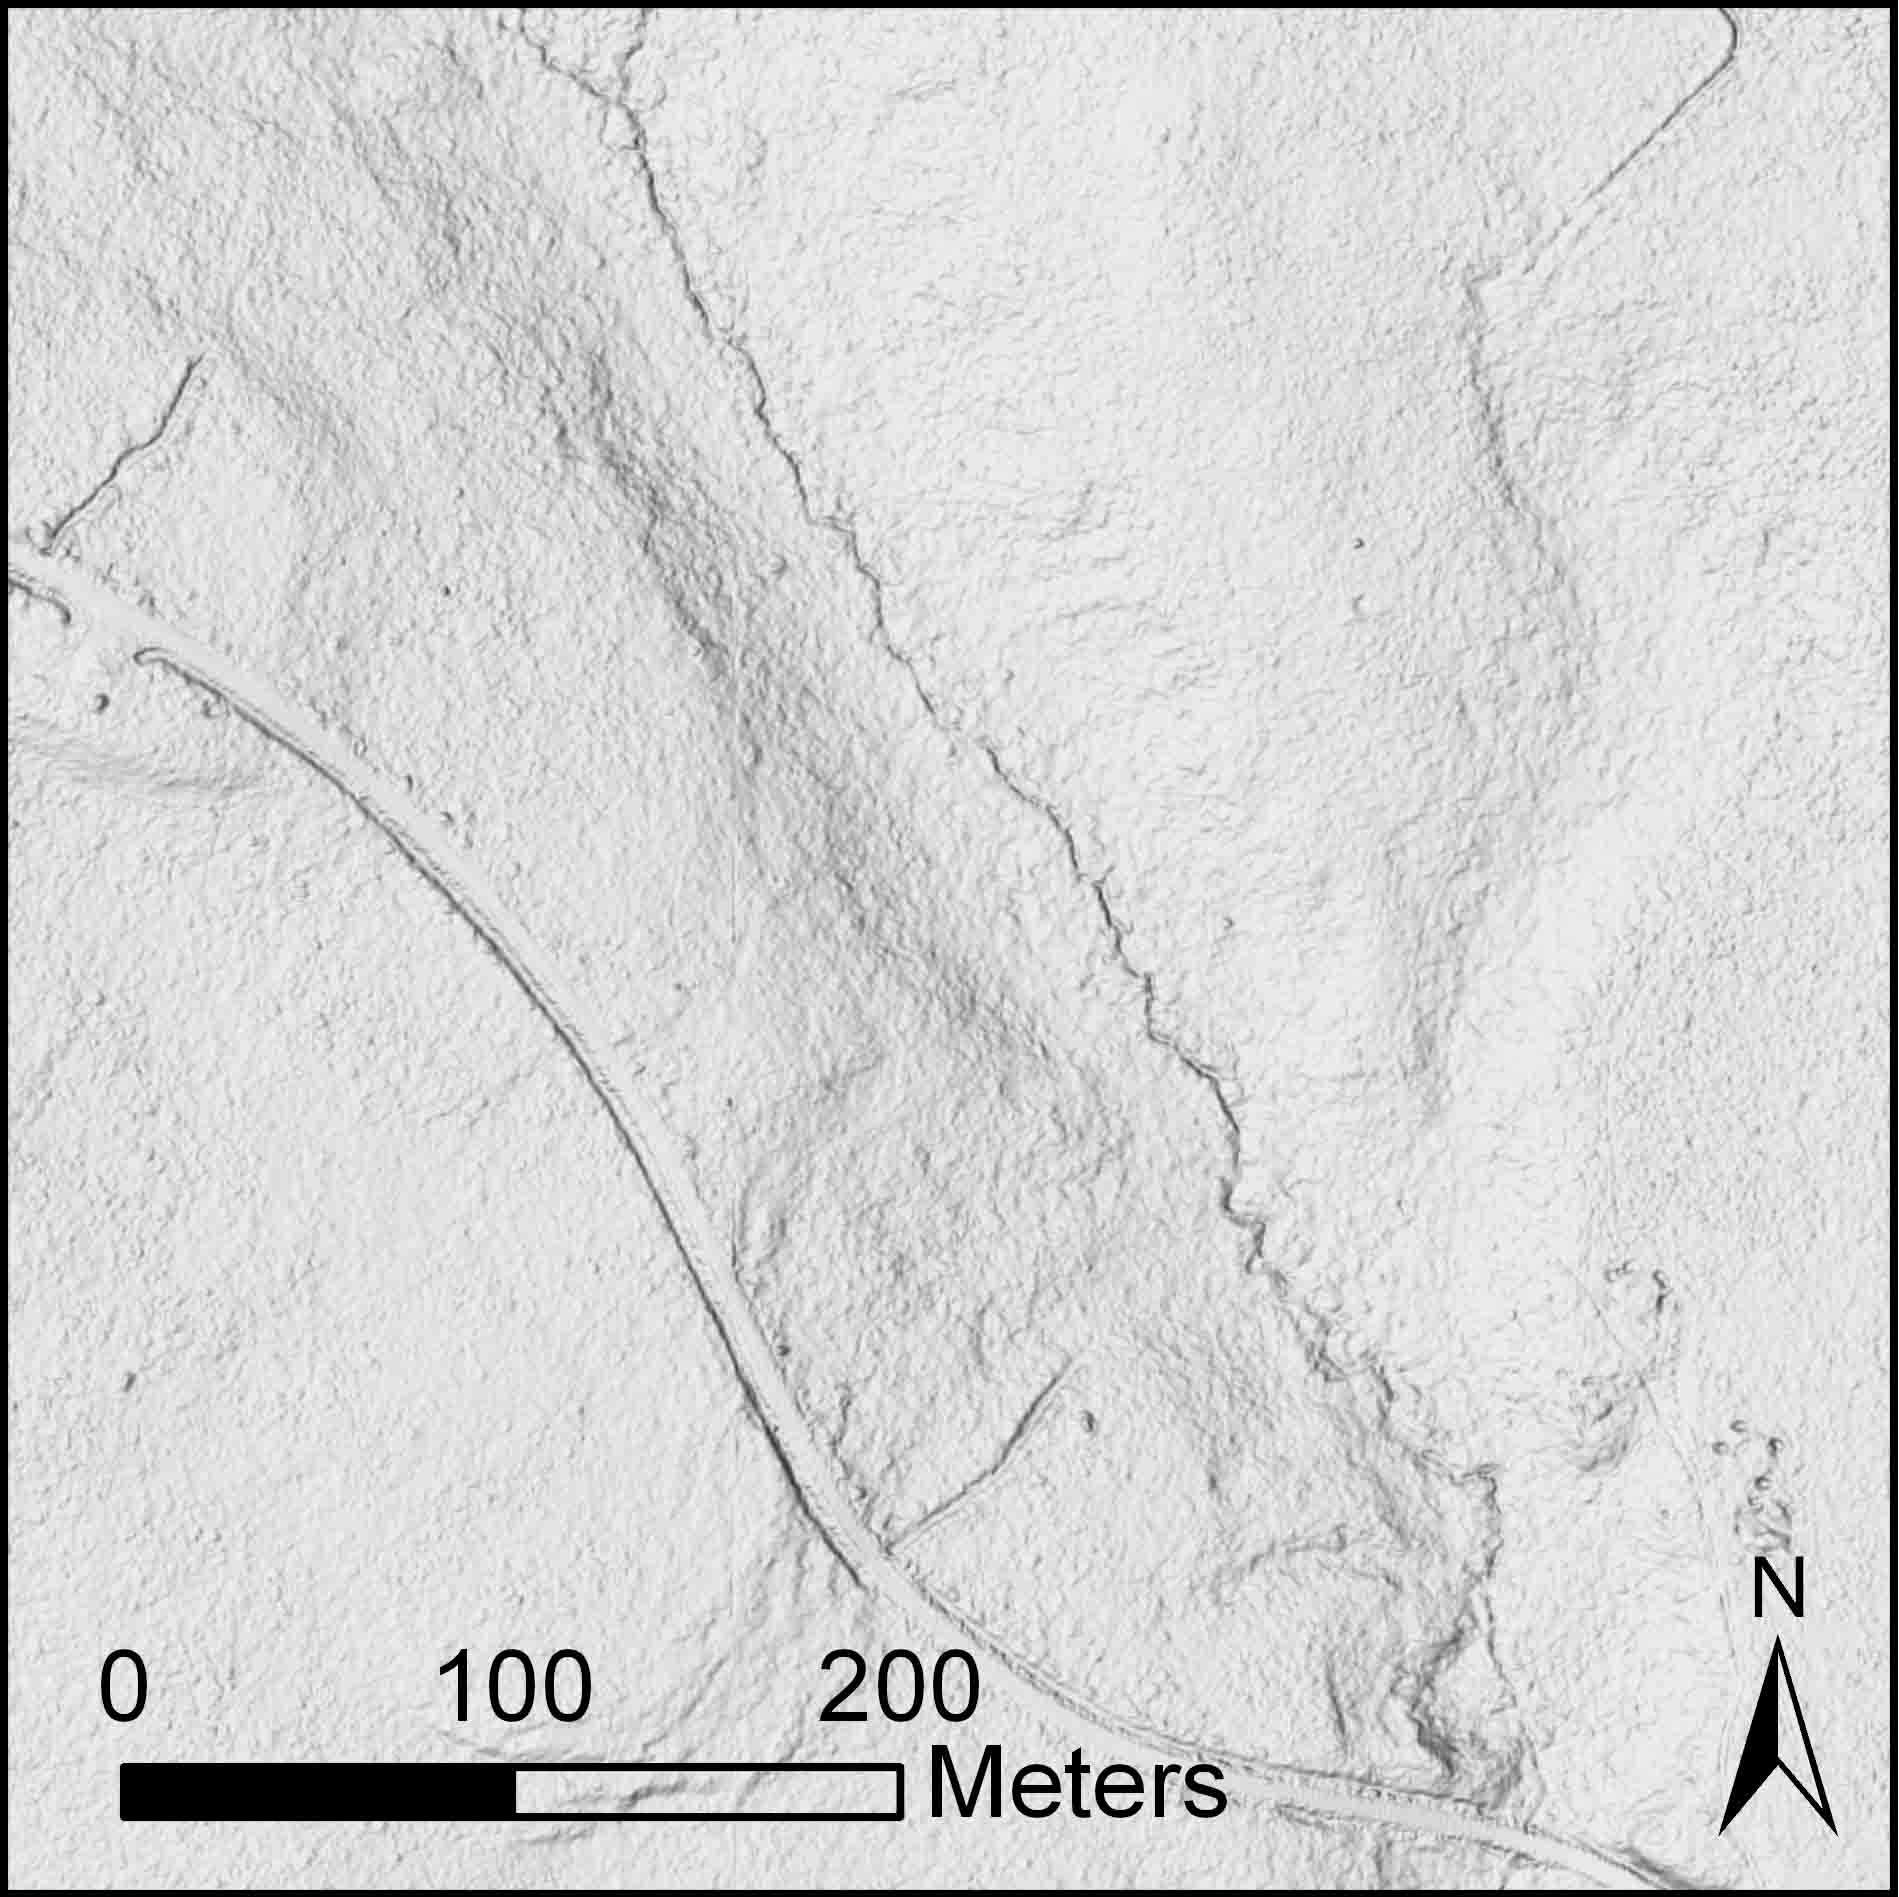
\includegraphics{./images/results_illustration_1_lo.jpg}}}%%%
\DIFdelFL{\hspace{5pt}
    }%DIFDELCMD < \subfigure[]{
%DIFDELCMD <         \resizebox*{5.5cm}{!}{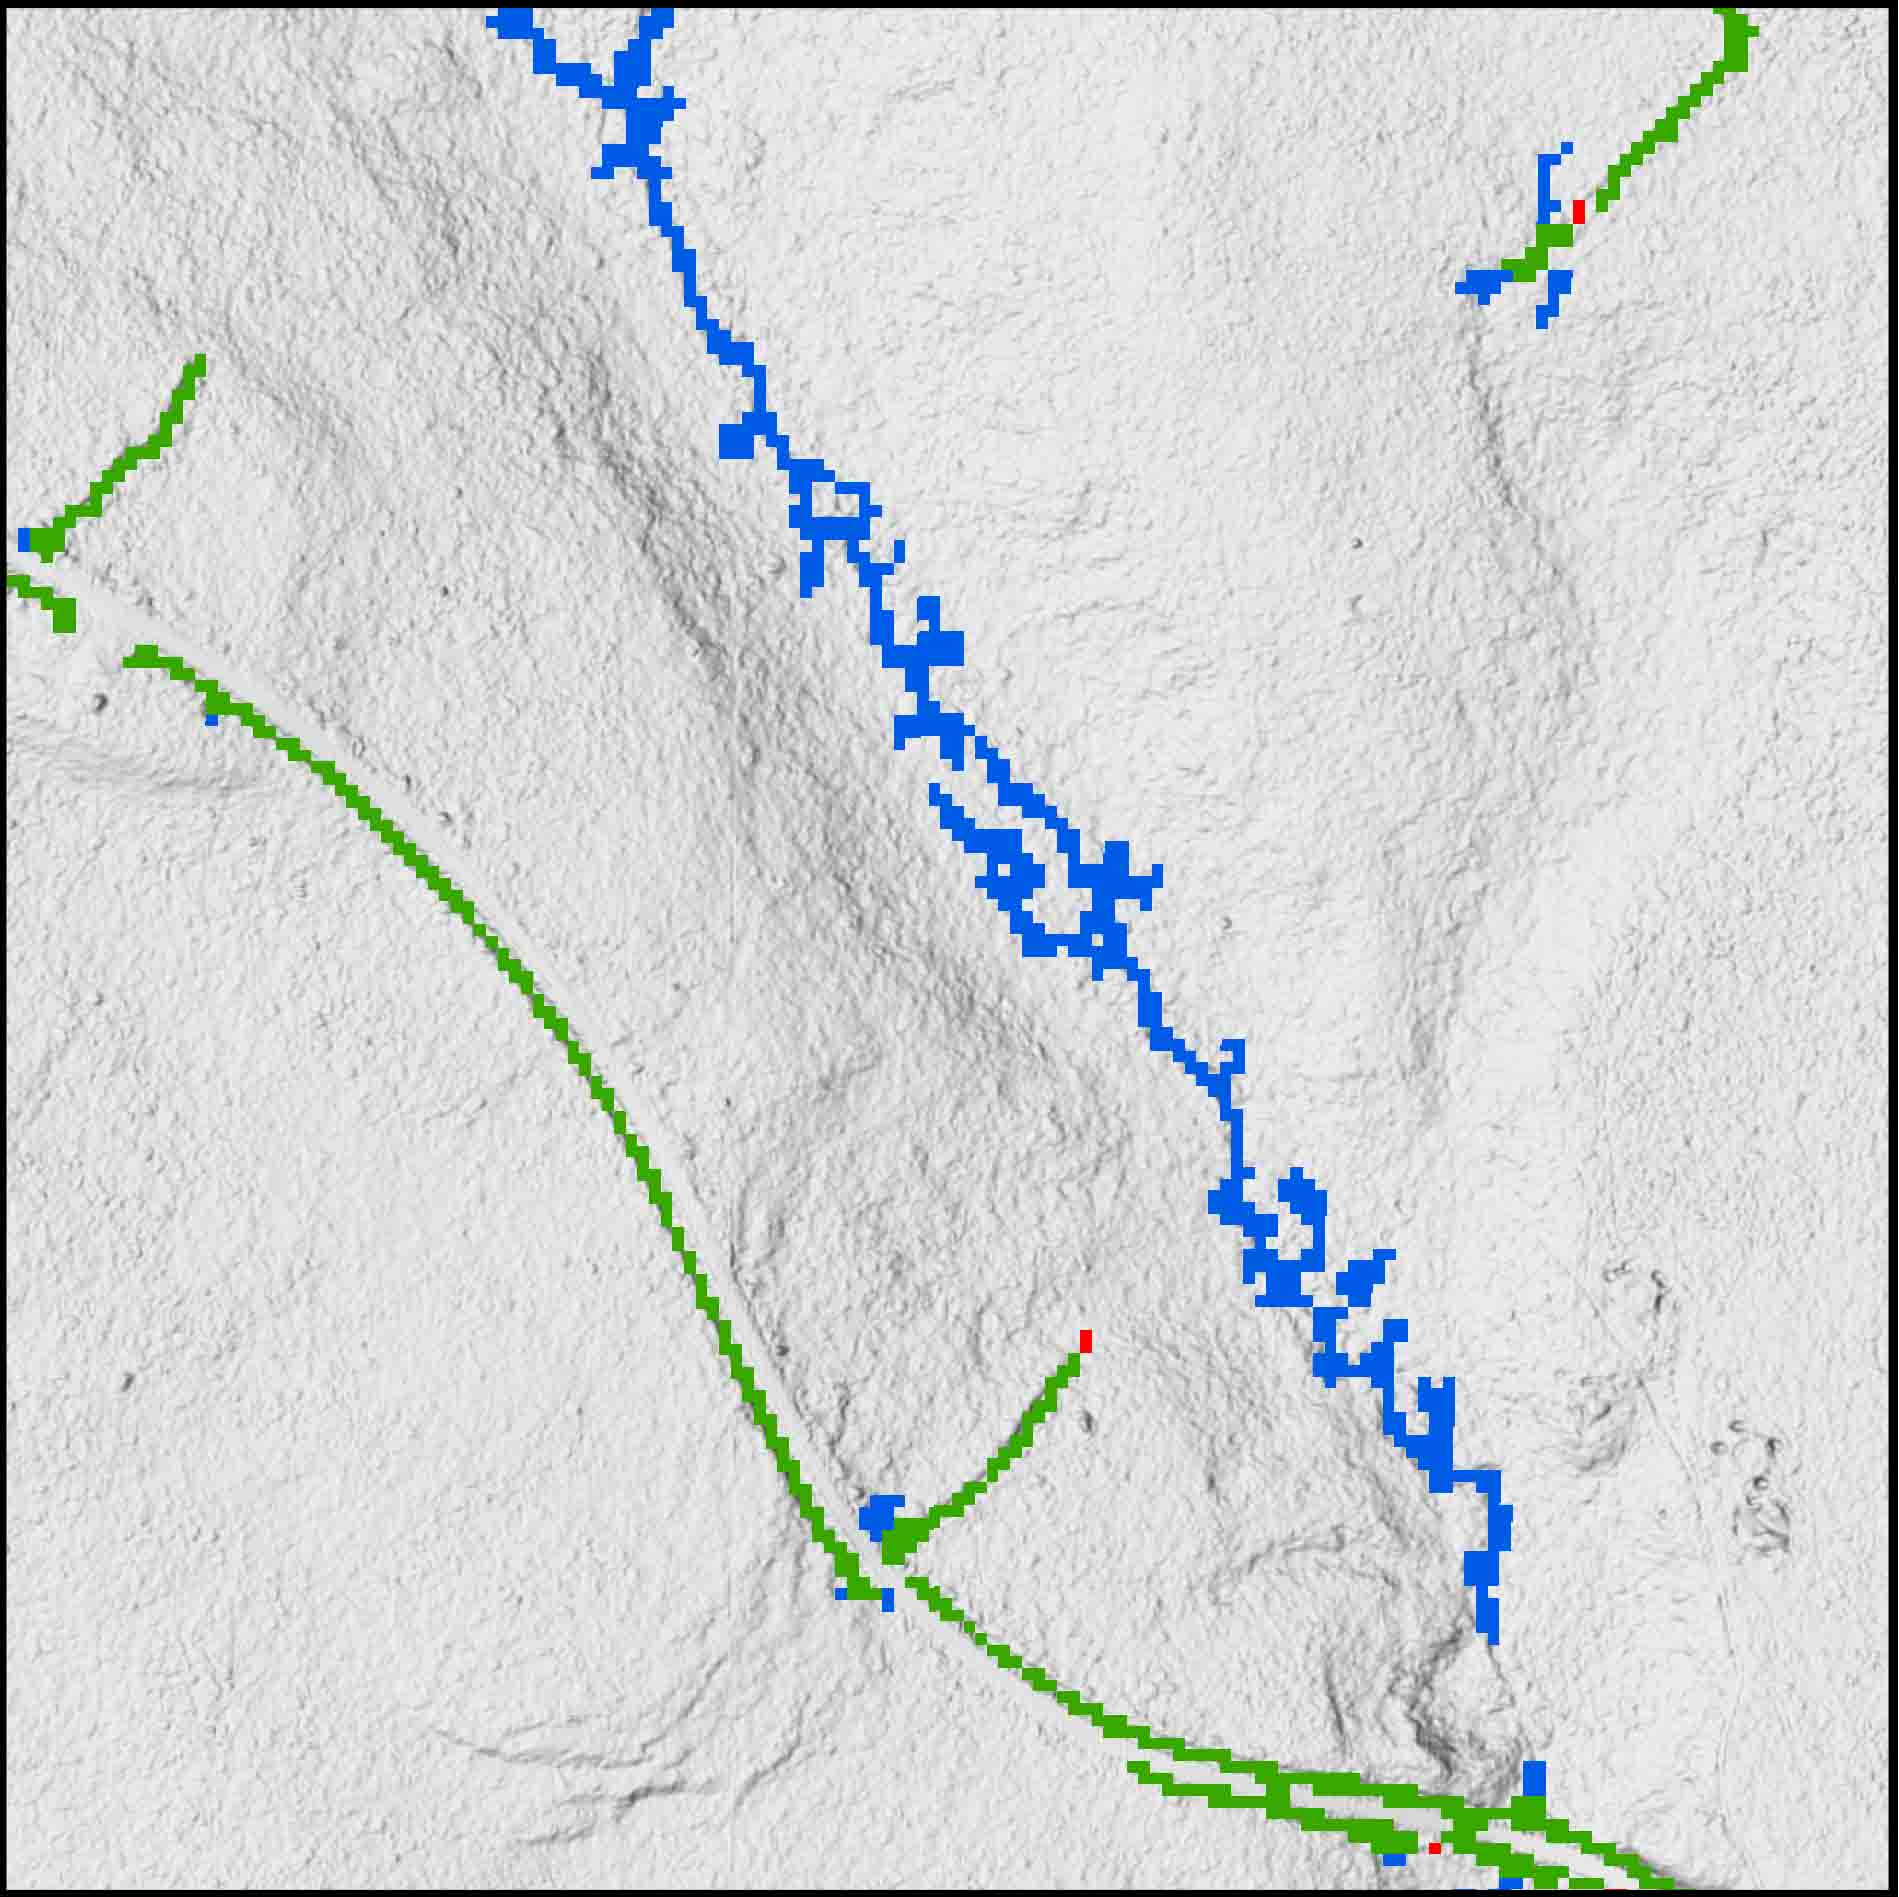
\includegraphics{./images/results_illustration_2_lo.jpg}}}
%DIFDELCMD <     \subfigure[]{
%DIFDELCMD <         \resizebox*{5.5cm}{!}{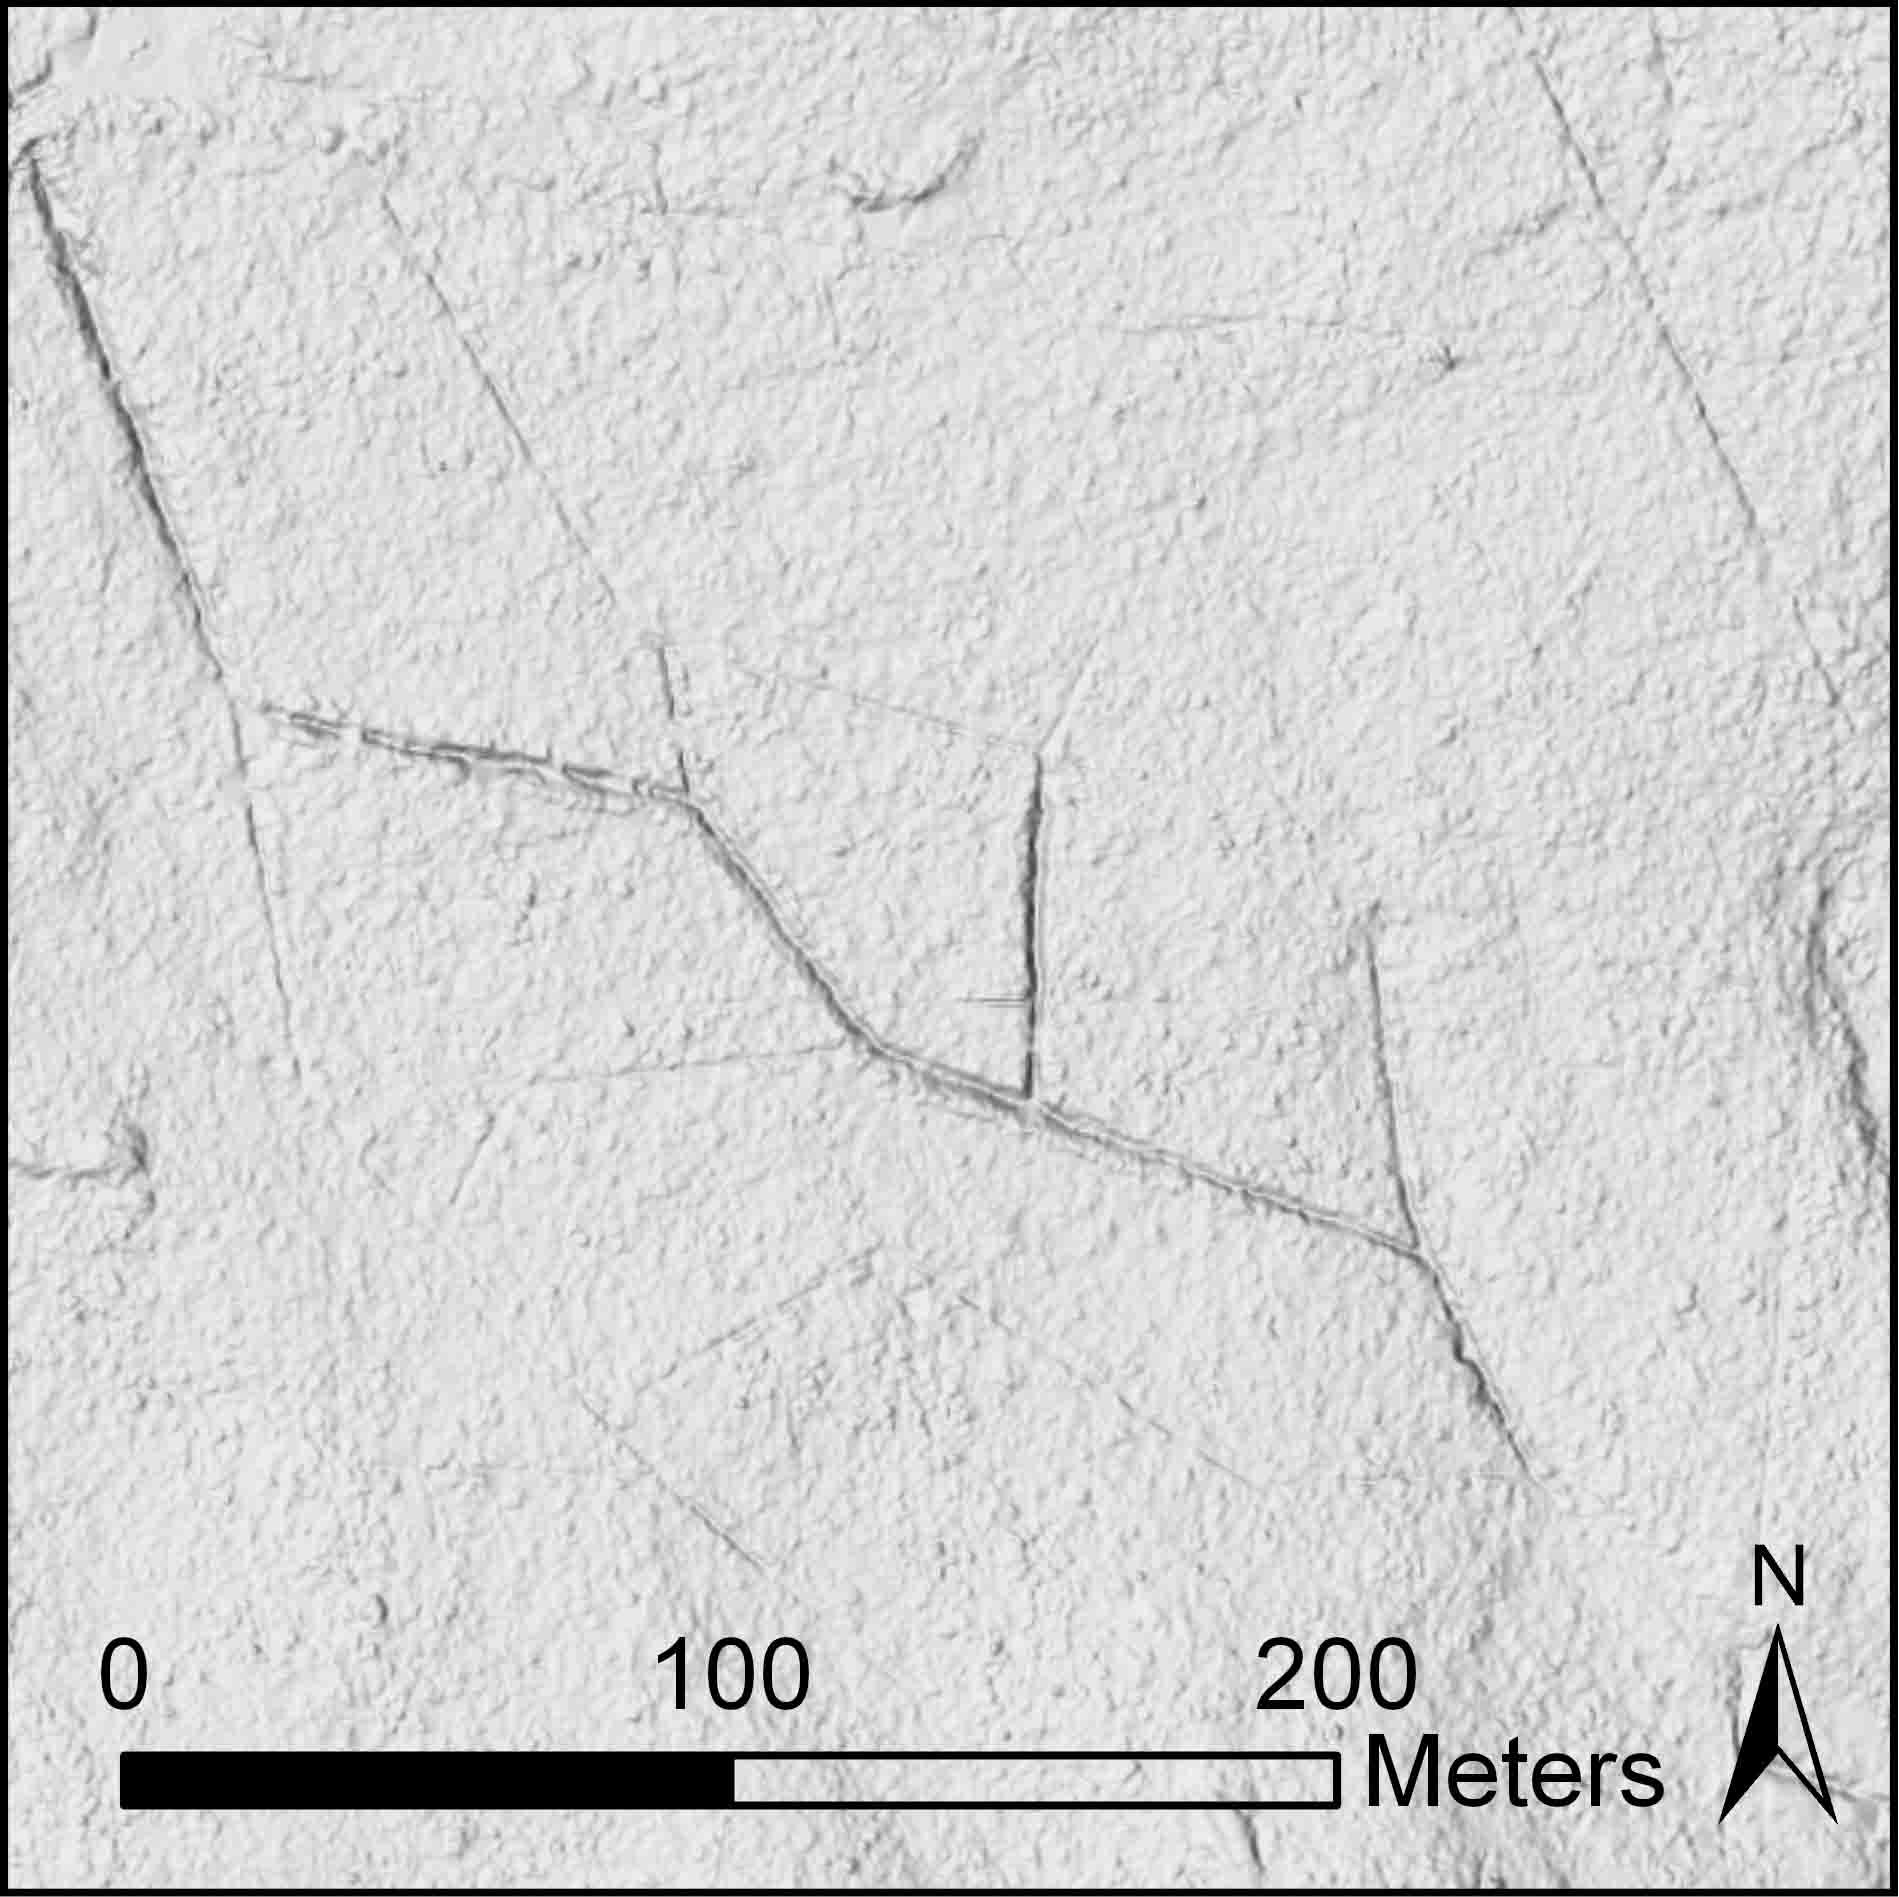
\includegraphics{./images/results_illustration_3_lo.jpg}}}%%%
\DIFdelFL{\hspace{5pt}
    }%DIFDELCMD < \subfigure[]{
%DIFDELCMD <         \resizebox*{5.5cm}{!}{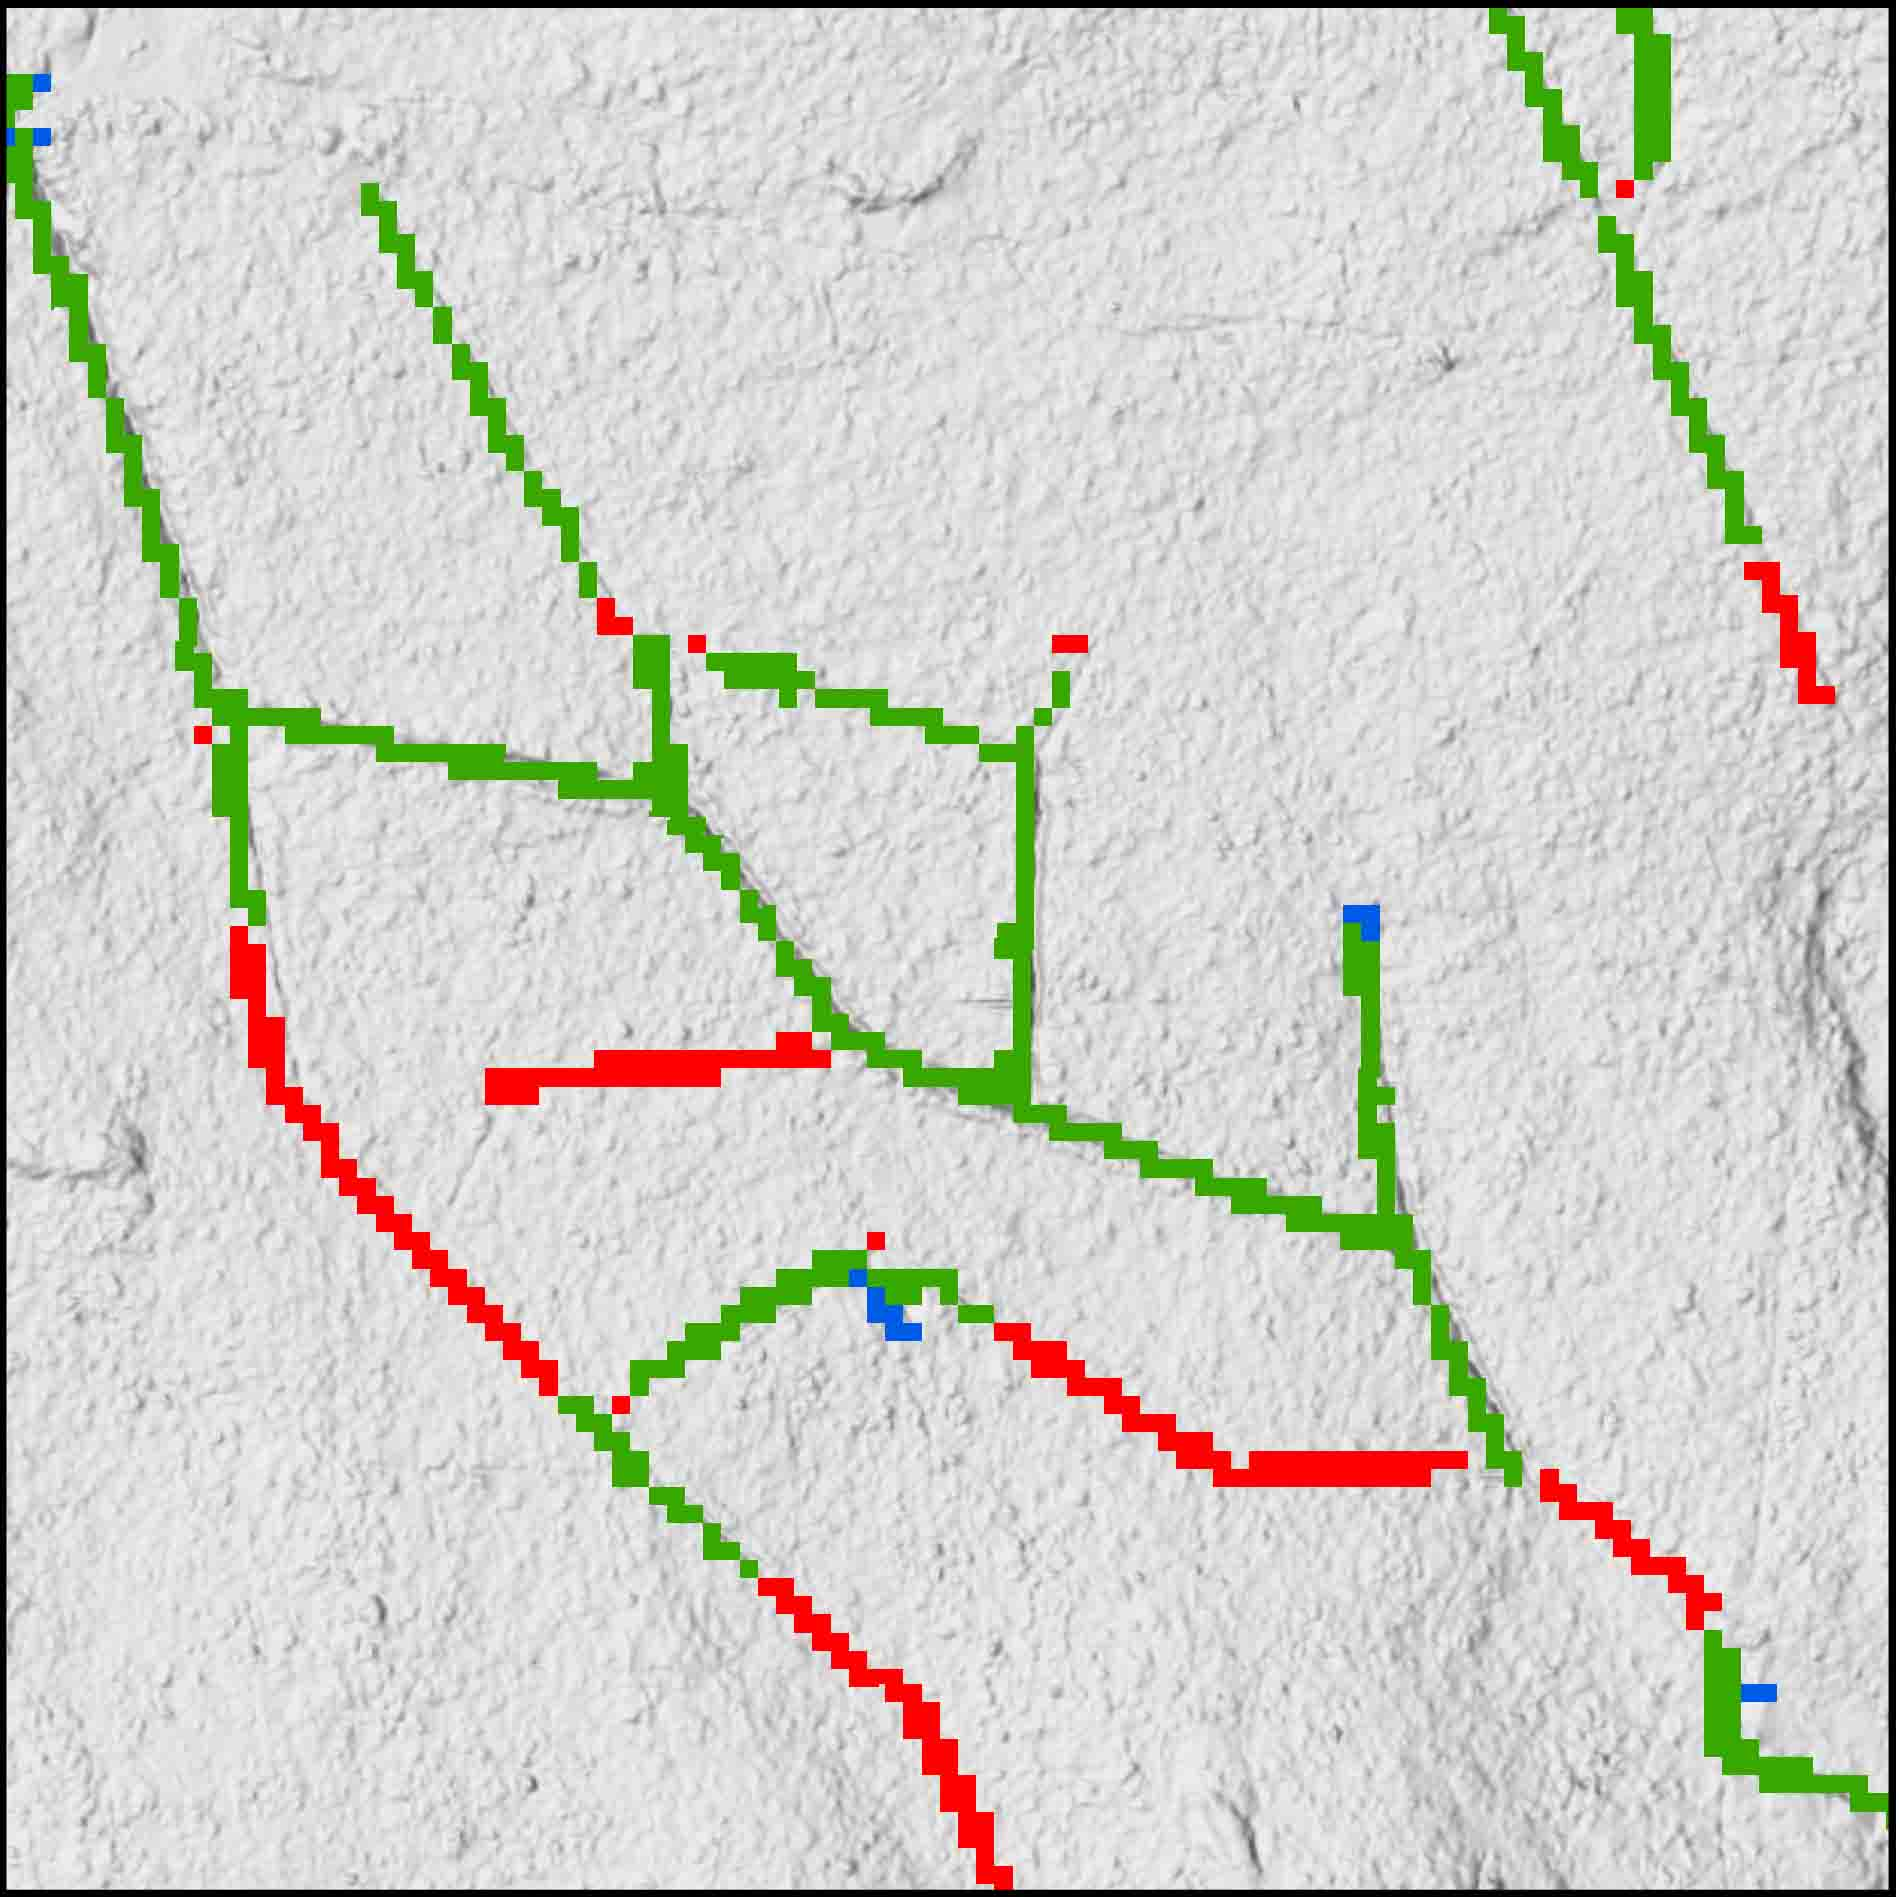
\includegraphics{./images/results_illustration_4_lo.jpg}}}
%DIFDELCMD <     \subfigure[]{
%DIFDELCMD <         \resizebox*{5.5cm}{!}{\includegraphics{./images/results_illustration_5_lo.jpg}}}%%%
\DIFdelFL{\hspace{5pt}
    }%DIFDELCMD < \subfigure[]{
%DIFDELCMD <         \resizebox*{5.5cm}{!}{\includegraphics{./images/results_illustration_6_lo.jpg}}}
%DIFDELCMD <     %%%
\DIFdelendFL \DIFaddbeginFL \subfigure[]{
        \resizebox*{4cm}{!}{\includegraphics{./images/results_illustration_1_lo.jpg}}}\DIFaddFL{\hspace{5pt}
    }\subfigure[]{
        \resizebox*{4cm}{!}{\includegraphics{./images/results_illustration_2_lo.jpg}}}
    \newline \subfigure[]{
        \resizebox*{4cm}{!}{\includegraphics{./images/results_illustration_3_lo.jpg}}}\DIFaddFL{\hspace{5pt}
    }\subfigure[]{
        \resizebox*{4cm}{!}{\includegraphics{./images/results_illustration_4_lo.jpg}}}
    \newline \subfigure[]{
        \resizebox*{4cm}{!}{\includegraphics{./images/results_illustration_5_lo.jpg}}}\DIFaddFL{\hspace{5pt}
    }\subfigure[]{
        \resizebox*{4cm}{!}{\includegraphics{./images/results_illustration_6_lo.jpg}}}
    \newline
    \DIFaddendFL \caption{\DIFaddbeginFL \textbf{\DIFaddFL{Visual analysis of ditch detector.}} \DIFaddendFL The left panel shows the hillshade for a number of subsections, and the right panel shows the hillshade with the extracted ditches superimposed on top. Green marks correctly classified ditches (true positives), red marks missed ditches (false negatives), blue marks incorrectly classified ditches (false positives), and transparent areas mark correctly classified non-ditches (true negatives). \textbf{a} and \textbf{b} illustrate that the most common false positives were natural stream channels being classified as ditches. \textbf{c} and \textbf{d} illustrate that very shallow ditches that were barely visible in the DEM were not captured with our ditch detector. \textbf{e} and \textbf{f} illustrate that some of the deepest and more prominent ditches were also missed. This occurred as a result of attempting to get rid of more false positives in the form of streams by using the \DIFdelbeginFL \DIFdelFL{input variables, as }\DIFdelendFL \DIFaddbeginFL \DIFaddFL{features }\DIFaddendFL explained in \ref{impoundmentstreamremoval}.}
    \label{fig:resultsillustrations}
\end{figure}
\DIFdelbegin %DIFDELCMD < \clearpage
%DIFDELCMD < %%%
\DIFdelend 

In \hyperref[featureimportancetable]{Table} \ref{featureimportancetable}, the top 20 (out of 40) \DIFdelbegin \DIFdel{input variables }\DIFdelend \DIFaddbegin \DIFadd{features }\DIFaddend from the Random Forests \DIFdelbegin \DIFdel{models }\DIFdelend \DIFaddbegin \DIFadd{model }\DIFaddend are presented with their \DIFdelbegin \DIFdel{importance percentages for the models making a successful prediction. Input variables based on HPMF and Impoundment Index }\DIFdelend \DIFaddbegin \DIFadd{Gini importances \mbox{%DIFAUXCMD
\citep{gini}}\hspace{0pt}%DIFAUXCMD
. Features derived from the }\hyperref[hpmf]{HPMF} \DIFadd{and }\hyperref[impoundment]{Impoundment} \DIFadd{terrain indices }\DIFaddend contributed the most to a successful prediction. The \DIFdelbegin \DIFdel{Gini importance was obtained using the Gini impurity for each variable \mbox{%DIFAUXCMD
\citep{gini}}\hspace{0pt}%DIFAUXCMD
}\DIFdelend \DIFaddbegin \DIFadd{features that used statistical aggregation methods on the neighbouring area around pixels, as well as the stream removal and Gabor filter features also performed well}\DIFaddend .

\begin{table} [!htb]
\DIFdelbeginFL %DIFDELCMD < \tbl{The top 20 input variables (out of 40) by importance when the models make a prediction.}
%DIFDELCMD <         %%%
\DIFdelendFL \DIFaddbeginFL \centering
    \DIFaddendFL {\DIFdelbeginFL %DIFDELCMD < \begin{tabular}{llr}
%DIFDELCMD <           \toprule
%DIFDELCMD <           %%%
\DIFdelFL{Position }\DIFdelendFL \DIFaddbeginFL \begin{tabular}{r|ll}
      \DIFaddFL{Pos }\DIFaddendFL & Variable\textsuperscript{a} & Importance (\%) \\
      \DIFdelbeginFL %DIFDELCMD < \midrule
%DIFDELCMD <           %%%
\DIFdelendFL \DIFaddbeginFL \hline
      \DIFaddendFL 1.  & Impoundment mean 3                                  & 7.33\\
      2.  & HPMF mean 4                                         & 6.23\\
      3.  & Impoundment mean 4                                  & 5.57\\
      4.  & Impoundment mean 2                                  & 5.41\\
      5.  & HPMF mean 3                                         & 4.33\\
      6.  & Impoundment median 4                                & 3.84\\
      7.  & HPMF Gabor - streams removed                        & 3.54\\
      8.  & HPMF median 4                                       & 3.40\\
      9.  & Impoundment median 2                                & 3.01\\
      10. & Sky View Factor Gabor - streams removed             & 2.84\\
      11. & HPMF mean 6                                         & 2.73\\
      12. & Impoundment median 6                                & 2.69\\
      13. & Impoundment standard deviation 4                    & 2.52\\
      14. & Sky View Factor Gabor                               & 2.44\\
      15. & Impoundment ditch amplification                     & 2.43\\
      16. & Impoundment mean 6                                  & 2.27\\
      17. & Impoundment ditch amplification - streams removed   & 2.24\\
      18. & HPMF min 2                                          & 2.23\\
      19. & Slope standard deviation 6                          & 2.01\\
      20. & Sky View Factor non-ditch amplification             & 1.88\\
      \DIFdelbeginFL %DIFDELCMD < \bottomrule
%DIFDELCMD <         %%%
\DIFdelendFL \DIFaddbeginFL \hline
    \DIFaddendFL \end{tabular}}
    \DIFdelbeginFL %DIFDELCMD < \tabnote{\textsuperscript{a} The number next to some of the variables indicates the circular radius used to select \newline what neighbouring pixels to use in the statistical aggregation method. The radii\newline \mbox{represents pixels with a 0.5 m resolution.\itshape\ignorespaces}}
%DIFDELCMD <     %%%
\DIFdelendFL \DIFaddbeginFL \caption{\textbf{\DIFaddFL{Feature importances.}} \DIFaddFL{The top 20 features (out of 40) by Gini importance. }\newline \DIFaddFL{\textsuperscript{a} The number next to some of the variables indicates the circular radius used to select what neighbouring pixels to use in the statistical aggregation method. The radii represents pixels with a 0.5 m resolution.}}
    \DIFaddendFL \label{featureimportancetable}
\end{table}

\section{Discussion}

\DIFdelbegin \DIFdel{The comparison with the field observed channels and the available maps clearly indicate the need for better maps of ditches, as only 9\% of ditches are mapped.  (}%DIFDELCMD < \hyperref[fig:watercoursebarplot]{Figure} %%%
\DIFdel{\ref{fig:watercoursebarplot}). }\DIFdelend Our study has shown that it is possible to locate ditches automatically in high-resolution DEMs ($0.5  * 0.5 $ metres, in our case), and that more of the ditches can be detected if \DIFdelbegin \DIFdel{the information from }\DIFdelend several terrain indices (\DIFdelbegin %DIFDELCMD < \hyperref[recreatedpredictionperformance]{Table} %%%
\DIFdel{\ref{recreatedpredictionperformance}) is }\DIFdelend \DIFaddbegin \hyperref[predictionperformance]{Table} \DIFadd{\ref{predictionperformance}) are }\DIFaddend combined through machine learning than if indices are used separately (\DIFdelbegin %DIFDELCMD < \hyperref[predictionperformance]{Table} %%%
\DIFdel{\ref{predictionperformance}}\DIFdelend \DIFaddbegin \hyperref[recreatedpredictionperformance]{Table} \DIFadd{\ref{recreatedpredictionperformance}}\DIFaddend ). The ditch detection performance varied depending on the type of ditches, this is illustrated in \hyperref[fig:ditchpictures]{Figure} \ref{fig:ditchpictures}. For example, the retrieval rate was slightly higher for the road ditches compared to forest or agricultural ditches. This is likely due to the fact that  road ditches are found in open areas alongside roads, and also,   they are generally well maintained for optimum functioning (\hyperref[fig:ditchpictures]{Figure} \ref{fig:ditchpictures} \hyperref[fig:ditchpictures]{a}). However, most of the ditches in Krycklan today are found below the canopy (e.g. \hyperref[fig:ditchpictures]{Figure} \ref{fig:ditchpictures} \hyperref[fig:ditchpictures]{c}), and the majority have not been maintained, causing difficulties in detecting them as some have grown back in with peat, grasses, or shrubs (\hyperref[fig:resultstreesbushes]{Figure} \ref{fig:resultstreesbushes} \hyperref[fig:resultstreesbushes]{b}). This, in combination with the surrounding peat having subsided \citep{heikurainen}, have rendered them almost impossible to detect in the DEM today (\hyperref[fig:ditchpictures]{Figure} \ref{fig:ditchpictures} \hyperref[fig:ditchpictures]{d}). Despite these issues we had a recall rate of 70.28\%, showing that the majority of the ditches could still be retrieved automatically.


\begin{figure} [!htb]
\centering
    \DIFdelbeginFL %DIFDELCMD < \subfigure[]{
%DIFDELCMD <         \resizebox*{6.85cm}{!}{\includegraphics{./images/road_ditch_lo.jpg}}}%%%
\DIFdelFL{\hspace{7pt}
    }%DIFDELCMD < \subfigure[]{
%DIFDELCMD <         \resizebox*{6.85cm}{!}{\includegraphics{./images/mire_ditch_lo.jpg}}}
%DIFDELCMD <     \subfigure[]{
%DIFDELCMD <         \resizebox*{6.85cm}{!}{\includegraphics{./images/forest_ditch_lo.jpg}}}%%%
\DIFdelFL{\hspace{7pt}
    }%DIFDELCMD < \subfigure[]{
%DIFDELCMD <         \resizebox*{6.85cm}{!}{\includegraphics{./images/overgrown_ditch_lo.jpg}}}
%DIFDELCMD <     %%%
\DIFdelendFL \DIFaddbeginFL \subfigure[]{
        \resizebox*{6cm}{!}{\includegraphics{./images/road_ditch_lo.jpg}}}
    \subfigure[]{
        \resizebox*{6cm}{!}{\includegraphics{./images/mire_ditch_lo.jpg}}}
    \subfigure[]{
        \resizebox*{6cm}{!}{\includegraphics{./images/forest_ditch_lo.jpg}}}
    \subfigure[]{
        \resizebox*{6cm}{!}{\includegraphics{./images/overgrown_ditch_lo.jpg}}}
    \DIFaddendFL \caption{\DIFdelbeginFL \DIFdelFL{All }\DIFdelendFL \DIFaddbeginFL \textbf{\DIFaddFL{Ditches in the study catchment.}} \DIFaddFL{These }\DIFaddendFL photos \DIFdelbeginFL \DIFdelFL{show ditches in the study catchment. They }\DIFdelendFL illustrate the difficulty of capturing the ditches based on their form (i.e. an elongated, narrow, hollow in the ground). \textbf{a: }A roadside ditch. These are generally easily detected as they are usually found in open areas along the roads, and have often been maintained. \textbf{b: }A ditch in a mire; this is still easily detected, as there is no canopy and there is a clear elevation difference between the ditch and surrounding area. \textbf{c: }A narrow, more or less  overgrown ditch in a dense forest stand. \textbf{d: }A ditch in a mire that has more or less grown back in with \textit{Sphagnum sp.} and \textit{Carex}, likely also in combination with subsiding surrounding soils. Such ditches can be found in the field as the vegetation differs, but as there is no longer an elevation difference between the ditch and the surrounding soils it will not be detected in the DEM. \DIFaddbeginFL \newline \DIFaddendFL Photos a-c: E. Maher Hasselquist\DIFaddbeginFL \DIFaddFL{, }\DIFaddendFL Photo d: G. Norstedt\DIFaddbeginFL \DIFaddFL{.}\DIFaddendFL }
    \label{fig:ditchpictures}
\end{figure}
\clearpage

Hypothetically, it should be quite easy to detect ditches using LiDAR data. In practice, however, there are many variables affecting the results, such as the point density and the interpolation method used to create the DEM. \citet{rapinel} found that the results were usually more sensitive to the point density (ranging 1-4 points $m^{2}$ in their study) than the interpolation method. They retrieved 54.8 and 63.8 \% of the ditches on the \DIFdelbegin \DIFdel{Acuey and Boucey marches }\DIFdelend \DIFaddbegin \DIFadd{Aucey and Boucey marshes }\DIFaddend in France, compared to 70.28 \% in our study. However, in our study we had a \DIFaddbegin \DIFadd{LiDAR }\DIFaddend point density of 20 points $m^{2}$, so the quality of the DEM in our study ought to be robust, which may have contributed to our higher retrieval rate. \hyperref[fig:resultstreesbushes]{Figure} \ref{fig:resultstreesbushes} \hyperref[fig:resultstreesbushes]{(a, b)} illustrates the difference in the quality of the \DIFdelbegin \DIFdel{LiDAR data }\DIFdelend \DIFaddbegin \DIFadd{ground DEM when it is generated from LiDAR }\DIFaddend where the laser pulses have caught in trees or shrubs\DIFdelbegin \DIFdel{. When too few LiDAR points reach the ground, the DEM generation is forced to interpolate over a larger area, leading to inaccuracies in the ground DEM}\DIFdelend \DIFaddbegin \DIFadd{, and fewer points have reached the ground}\DIFaddend .

\DIFdelbegin %DIFDELCMD < \begin{figure} [%%%
\DIFdelFL{!htb}%DIFDELCMD < ]
%DIFDELCMD <     %%%
\DIFdelendFL \DIFaddbeginFL \begin{figure}[!htb]
\DIFaddendFL \centering
    \DIFdelbeginFL %DIFDELCMD < \subfigure[]{
%DIFDELCMD <         \resizebox*{6.8cm}{!}{\includegraphics{./images/results_trees_bushes_1_lo.jpg}}}%%%
\DIFdelFL{\hspace{7pt}
    }%DIFDELCMD < \subfigure[]{
%DIFDELCMD <         \resizebox*{6.8cm}{!}{\includegraphics{./images/results_trees_bushes_2_lo.jpg}}}
%DIFDELCMD <     \subfigure[]{
%DIFDELCMD <         \resizebox*{6.8cm}{!}{\includegraphics{./images/results_trees_bushes_3_lo.jpg}}}%%%
\DIFdelFL{\hspace{7pt}
    }%DIFDELCMD < \subfigure[]{
%DIFDELCMD <         \resizebox*{6.8cm}{!}{\includegraphics{./images/results_trees_bushes_4_lo.jpg}}}
%DIFDELCMD <     %%%
\DIFdelendFL \DIFaddbeginFL \subfigure[]{
        \resizebox*{5.5cm}{!}{\includegraphics{./images/results_trees_bushes_1_lo.jpg}}}\DIFaddFL{\hspace{7pt}
    }\subfigure[]{
        \resizebox*{5.5cm}{!}{\includegraphics{./images/results_trees_bushes_2_lo.jpg}}}
    \subfigure[]{
        \resizebox*{5.5cm}{!}{\includegraphics{./images/results_trees_bushes_3_lo.jpg}}}\DIFaddFL{\hspace{7pt}
    }\subfigure[]{
        \resizebox*{5.5cm}{!}{\includegraphics{./images/results_trees_bushes_4_lo.jpg}}}
    \DIFaddendFL \caption{\DIFaddbeginFL \textbf{\DIFaddFL{Weak LiDAR scan illustration.}} \DIFaddendFL \textbf{a} and \textbf{b} illustrate that despite a \DIFaddbeginFL \DIFaddFL{LiDAR }\DIFaddendFL point density of 20 points $m^2$, not all points reach the ground in places with dense vegetation. In \textbf{a} there is a clear difference between the smooth surface of the DEM in the open area (black arrow), and in the areas covered by trees and shrubs (red arrows), where the DEM is much coarser due to interpolation with a lower number of LiDAR points here. The orthophoto (\textbf{b}), clearly shows that trees and shrubs are growing in the ditches in this area\DIFdelbeginFL \DIFdelFL{. This makes }\DIFdelendFL \DIFaddbeginFL \DIFaddFL{, making }\DIFaddendFL it more difficult to detect ditches. However, despite these coarser grid points in the DEM, \textbf{c} and \textbf{d} shows that the ditch detector still managed to capture a majority of the ditches (green), and only failed at certain points (red).}
    \label{fig:resultstreesbushes}
\end{figure}

\DIFdelbegin \DIFdel{With our method, natural streams were often classified as false positives }\DIFdelend \DIFaddbegin \DIFadd{A common false positive with our ditch detector is natural streams }\DIFaddend (\hyperref[fig:resultsillustrations]{Figure} \ref{fig:resultsillustrations} \hyperref[fig:resultsillustrations]{b})\DIFdelbegin \DIFdel{as our aim was focused on locating ditches}\DIFdelend . However, this indicates that \DIFaddbegin \DIFadd{with some adjustments, }\DIFaddend our method could also be used to map small, previously unmapped natural stream channels. The national survey showed that 55\% of the natural stream channels and 75\% of the straightened water courses were missing on the maps \DIFaddbegin \DIFadd{(}\autoref{fig:watercoursebarplot}\DIFadd{)}\DIFaddend . This is in line with other national \citep{kuglerova} and international \citep{benstead} studies highlighting this phenomenon called "Aqua Incognita - the unknown headwaters" \citep{bishop,kuglerova}.

\DIFdelbegin \DIFdel{The results from our method (}%DIFDELCMD < \hyperref[predictionperformance]{Table} %%%
\DIFdel{\ref{predictionperformance}) show that we managed to attain a Cohen's $\kappa$ rating in }\DIFdelend \DIFaddbegin \DIFadd{Sometimes pixels in ditches were initially identified correctly as ditch pixels, but because not enough pixels in the surrounding area were detected, }\DIFaddend the \DIFdelbegin \DIFdel{substantial range, according to performance thresholds proposed by \mbox{%DIFAUXCMD
\citet{kappaanalysis}}\hspace{0pt}%DIFAUXCMD
. The total recall value of 70.28 \% shows that we managed to find a majority of the ditch pixels that exist. The results of our method also showed a significant improvement for ditch detection over classifying with the digital terrain indices separately (}%DIFDELCMD < \hyperref[recreatedpredictionperformance]{Table} %%%
\DIFdel{\ref{recreatedpredictionperformance}). }\DIFdelend \DIFaddbegin \DIFadd{post-processing algorithms identified them as noise and removed them. However, these steps were necessary as they helped to remove small sinks or hilly areas that had been incorrectly classified as ditches. }\DIFaddend Had we been able to use labels that were correctly labelled on a pixel basis, i.e. each ditch had its actual width recorded, the \DIFdelbegin \DIFdel{models }\DIFdelend \DIFaddbegin \DIFadd{model }\DIFaddend could have learned with a better accuracy in the training phase, and the classification results would also most likely have benefitted from this. \DIFdelbegin %DIFDELCMD < 

%DIFDELCMD < %%%
\DIFdel{Sometimes pixels in ditches were initially identified correctly as ditch pixels, but because not enough pixels in the surrounding area were detected, the post-processing algorithms identified them as noise and removed them. Incorrectly classified ditch pixels that caused the precision to decrease were generally the pixels that lay in streams (}%DIFDELCMD < \hyperref[fig:resultsillustrations]{Figure} %%%
\DIFdel{\ref{fig:resultsillustrations} }%DIFDELCMD < \hyperref[fig:resultsillustrations]{a, b}%%%
\DIFdel{). However, small sinks or hilly areas incorrectly classified as ditches by the Random Forests models were generally removed in the post-processing. }\DIFdelend We managed to bridge gaps and exclude streams to some extent in our predictions. This was in part due to the post-processing of the \DIFdelbegin \DIFdel{prediction }\DIFdelend \DIFaddbegin \DIFadd{predictions }\DIFaddend helping where the \DIFdelbegin \DIFdel{models were unsuccessful on their }\DIFdelend \DIFaddbegin \DIFadd{model was unsuccessful on its }\DIFaddend own, and in part due to the \DIFdelbegin \DIFdel{input variables developed.
}%DIFDELCMD < \hyperref[featureimportancetable]{Table} %%%
\DIFdel{\ref{featureimportancetable} highlights the importance of the input variables that were developed by applying different statistical aggregations for neighbouring areas of pixels, similar to \mbox{%DIFAUXCMD
\citet{roelens}}\hspace{0pt}%DIFAUXCMD
, as well as the custom variables using filters such as the Impoundment stream removal or Gabor filters.
}\DIFdelend \DIFaddbegin \DIFadd{features developed.
}\DIFaddend 

One concern with our method \DIFdelbegin \DIFdel{was }\DIFdelend \DIFaddbegin \DIFadd{is }\DIFaddend that valuable information may have been discarded when aggregating the elevations from the original point cloud to a DEM. \citet{roelens} used  machine learning to detect ditches directly from point-clouds instead of a DEM. However, we achieved a similar score to their method; $\kappa=0.73$ in our study compared to 0.77 for grassland and 0.73 for peri-urban area in \citet{roelens} study. This suggests that DEM can also be used to automatically extract ditches, provided that enough input data is available to generate a high resolution DEM for capturing the small scale features of ditches. 

\citet{bailly} also showed that the vegetation cover significantly affects the ability to detect ditches from LiDAR data (\hyperref[fig:ditchpictures]{Figure} \ref{fig:ditchpictures} \& \ref{fig:resultstreesbushes}). Approximately 75\% of the ditches in their study were retrieved where no vegetation existed, whereas the detection accuracy went below 10\% under \DIFdelbegin \DIFdel{vegetation; especially when the ditches were covered by }\DIFdelend \DIFaddbegin \DIFadd{the cover of }\DIFaddend high vegetation, shrubs, and trees \citep{bailly}. \DIFdelbegin \DIFdel{Hence}\DIFdelend \DIFaddbegin \DIFadd{Thus}\DIFaddend , a $\kappa$ of 0.73 in our study \DIFaddbegin \DIFadd{catchment }\DIFaddend with 87\% forest cover \citep{krycklancatchment} is substantially better than that of previous research\DIFdelbegin \DIFdel{, and this could perhaps }\DIFdelend \DIFaddbegin \DIFadd{. This could possibly }\DIFaddend be a result of the higher point density of our LiDAR measurements (20 compared to 10 points \DIFaddbegin \DIFadd{per }\DIFaddend $m^{2}$). The hydrology of our study catchment also differs from that of other studies, as we have almost as many natural stream channels as ditches, whereas their studies were conducted in smaller, predominantly artificially drained areas \citep{bailly, roelens, rapinel}. Because our \DIFdelbegin \DIFdel{method }\DIFdelend \DIFaddbegin \DIFadd{model }\DIFaddend locates both ditches and natural stream channels, we have to take additional measures to remove the stream channels (affecting \DIFdelbegin \DIFdel{recall }\DIFdelend \DIFaddbegin \DIFadd{ditch detection }\DIFaddend negatively), as explained in \DIFaddbegin \hyperref[impoundmentstreamremoval]{section} \DIFaddend \ref{impoundmentstreamremoval}.

A future improvement to the ditch detector could be to use a shape index to remove small natural streams, as natural streams often form \DIFdelbegin \DIFdel{more complex channels}\DIFdelend \DIFaddbegin \DIFadd{complex channels, }\DIFaddend whereas ditches are often straight. A potential issue with generalising our ditch detector for use in other geographical areas is that \DIFdelbegin \DIFdel{all }\DIFdelend \DIFaddbegin \DIFadd{many of }\DIFaddend the post-processing steps and \DIFdelbegin \DIFdel{input variables }\DIFdelend \DIFaddbegin \DIFadd{features }\DIFaddend were developed based on occurrences in the Krycklan area. Different geographical compositions in other areas may require the adjustment of the thresholds used to fill gaps in ditches and to remove noise.

\section{Conclusion}

Detection of artificial ditches over large areas with substantial natural stream coverage is challenging, especially under tree canopy, but highly desired for effective forest management. Ditches represent elongated depressions in a DEM; however, the exact shape and size differs between ditches. We combined recently developed digital terrain indices (the most important being \DIFdelbegin \DIFdel{Impoundment }\DIFdelend \DIFaddbegin \hyperref[impoundment]{Impoundment} \DIFaddend Index and High Pass Medium Filter) but, unlike previous studies, did not apply generic thresholding on them. Instead, we included local variability in the indices by using different radii to capture ditches with varied shapes. This integration of a large set of terrain indices using machine learning produced good results, as evidenced by the confidence interval for the Cohen's $\kappa$ index\DIFdelbegin \DIFdel{ranging }\DIFdelend \DIFaddbegin \DIFadd{, which ranged }\DIFaddend from 0.655 to 0.781 with a confidence level of 95\%. With the developed \DIFdelbegin \DIFdel{input variables }\DIFdelend \DIFaddbegin \DIFadd{features }\DIFaddend and extensive post-processing, we also managed to remove many stream channels and fill gaps in the ditches where the LiDAR scans were weak. 

Although there is room for further improvement, the methodology is a significant step forward as it performed on a par with previous studies conducted in more homogeneous agricultural landscapes. Our approach enables accurate ditch detection in complex forested landscapes with tree canopy and many natural streams. Future work could introduce more \DIFdelbegin \DIFdel{input variables }\DIFdelend \DIFaddbegin \DIFadd{features }\DIFaddend and post-processing steps, such as using pathfinding algorithms to fill gaps in the ditch model or shape indices to remove stream channels from the prediction. Moving towards image segmentation instead of pixel classification of tabular pixel values could also be a suitable future approach. Our developed methodology can be adjusted to apply to any setting for artificial ditch detection, reducing time and labour investment compared to the conventional manual mapping techniques. The accurate ditch maps can \DIFaddbegin \DIFadd{both }\DIFaddend significantly contribute to practical forestry and operational land management\DIFdelbegin \DIFdel{at a landscape-scale.
}\DIFdelend \DIFaddbegin \DIFadd{, as well as allow government agencies, forest companies, and regional and local authorities to predict the climate consequences of potential management actions, which will be critical in reaching global sustainability goals.
}\DIFaddend 

\DIFdelbegin \section*{\DIFdel{Data and codes availability statement}}
%DIFAUXCMD
\DIFdel{The data and codes that support the findings of this study are available at the private links:}%DIFDELCMD < \newline
%DIFDELCMD < %%%
\DIFdel{\mbox{\href{https://figshare.com/s/23742e1f20fae3e404de}{https://figshare.com/s/23742e1f20fae3e404de} - Functions\itshape\ignorespaces}
\mbox{\href{https://figshare.com/s/741725088fe6292442c8}{https://figshare.com/s/741725088fe6292442c8} - Feature creation\itshape\ignorespaces}
\mbox{\href{https://figshare.com/s/f4e3bcf3bb2f8c18ecfa}{https://figshare.com/s/f4e3bcf3bb2f8c18ecfa} - Digital terrain indices experiment\itshape\ignorespaces}
\mbox{\href{https://figshare.com/s/88cd93c3b4aea6776c8b}{https://figshare.com/s/88cd93c3b4aea6776c8b} - Pilot experiment\itshape\ignorespaces}
\mbox{\href{https://figshare.com/s/60631095d26699f65f53}{https://figshare.com/s/60631095d26699f65f53} - Random Forests experiment\itshape\ignorespaces}
\mbox{\href{https://figshare.com/s/c0ae38ee5951498d21cd}{https://figshare.com/s/c0ae38ee5951498d21cd}} - Experiment data
}\DIFdelend \DIFaddbegin \section*{\DIFadd{CRediT authorship contribution statement}}
\DIFaddend 

\DIFdelbegin %DIFDELCMD < \label{lidartodem}
%DIFDELCMD < %%%
\DIFdel{The LiDAR dataset used in this study was produced by TerraTec Sweden AB in August 2015, on demand of the Department of Forest Resource Management at the Swedish University of Agricultural Sciences, and is freely available online at }%DIFDELCMD < \href{https://gis.krycklan.se/}{https://gis.krycklan.se/}%%%
\DIFdel{. The average density of the dataset was 20 pulses per $m^2$.  Ground point classification was performed with lasground (included in LAStools, a software suite produced by rapidlasso GmbH). The DEM was created with blast2dem (included in LAStools),  with cell size of $0.5*0.5$ m.
Only ground points were imported  to generate a DEM of the ground. This was conducted for 488 las-files of the study area that were mosaicked to one large file using Mosaic to new raster in Arc GIS Pro \mbox{%DIFAUXCMD
\citep{EsriArcGisBook}}\hspace{0pt}%DIFAUXCMD
}\DIFdelend \DIFaddbegin \hl{ Jag tolkar det som att denna sektion \"ar frivillig, men ESWA skriver i guiden att de uppmuntrar att man fyller i denna. De flesta artiklar jag har hittat listar h\"ar vad alla enskilda f\"orfattare har bidragit med. Kategorier: Conceptualization; Data curation; Formal analysis; Funding acquisition; Investigation; Methodology; Project administration; Resources; Software; Supervision; Validation; Visualization; Roles/Writing - original draft; Writing - review & editing.}

\section*{\DIFadd{Declaration of Competing Interest}}

\DIFadd{The authors declare that they have no known competing financial interests or personal relationships that could have appeared to influence the work reported in this paper}\DIFaddend .

\section*{Acknowledgements}
We wish to thank \DIFdelbegin \DIFdel{the two anonymous reviewers and }\DIFdelend Dr. Siddhartho Paul at the Swedish University of Agricultural Sciences, whose suggestions helped improve and clarify this manuscript. We also thank Sigurd Israelsson at the School of Engineering at J\"onk\"oping University for lending hardware resources for the experiments in this study. \DIFdelbegin \DIFdel{The work has been funded }\DIFdelend \DIFaddbegin \DIFadd{This work was supported }\DIFaddend by VINNOVA, EU InterReg Baltic Sea project WAMBAF tools and Formas. \DIFaddbegin \hl{ H\"ar ska varje grant definieras med "grant number[xxxx] efter varje akt\"or", jag tolkar det ocks\aa som att man ska skriva vilken roll varje finansi\"ar har.}
\DIFaddend 


\DIFdelbegin %DIFDELCMD < \label{references}
%DIFDELCMD < 

%DIFDELCMD < \bibliographystyle{tfv}
%DIFDELCMD < \bibliography{references.bib}
%DIFDELCMD < %%%
\DIFdelend \DIFaddbegin \bibliography{references}
\DIFaddend 

\end{document}
